\documentclass{article}
%%% important comment keywords %%%
% CAVEAT: -> a warning concerning some compilation issues that may break your system in some situation
% ADJUST: -> manual tweaks that you may want to change
% TODO: -> to-do list
% HACK: -> Savy macros to easily use a given packages

%%%%%%%%% Document language %%%%%%%%%
% \usepackage[utf8]{inputenc} % ADJUST: descomente esta linha para mudar o idioma do texto para Português
% \usepackage[portuguese]{babel}
% \usepackage{cmap} % must be loaded before fontenc; embeds a proper ToUnicode CMap so copy-pasted text from the PDF isn't garbled
% \usepackage[T1]{fontenc} % single-glyph accented characters (instead of OT1's composite accents), required together with cmap for correct copy-paste

%%%%%%%%% bibliography %%%%%%%%%
\usepackage[style=numeric-comp,backend=biber]{biblatex} % tells LaTeX to use the biber tool instead of the traditional bibtex tool for sorting and formatting your bibliography. Biber is a more advanced and powerful tool than bibtex and it provides more features, such as advanced sorting, Unicode support and support for various data sources.
\addbibresource{refs.bib} % add reference file, in the document, add \printbibliography to print bibliography

%%%%%%%%% references (cite and glossary) %%%%%%%%%
\makeatletter
% some classes (e.g., beamer) loads hyperref by default. So it is sensible to check whether it wasn't already loaded to avoind clashes
\@ifpackageloaded{hyperref}{
    % The package is already loaded
}{
    % The package is not loaded, so load it now
    \usepackage[colorlinks=true,hyperindex=false]{hyperref} % make references blue and clickable
}
\makeatother
\hypersetup{ % you can use allcolors=blue in hyperref options instead this setup
    linkcolor=black,          % For \gls{} entries
    citecolor=blue,          % For \cite{} entries
}
\usepackage{glossaries} % \newglossaryentry{} entries. ADJUST: If you want to make the glossary entries nonclickable, load this package before hyperref
% CAVEAT: don't use `glossaries-extra`, otherwise the conditional glossary entry will not work! % SEE: https://tex.stackexchange.com/questions/98494/glossaries-dont-print-single-occurences/230664#230664
\glsenableentrycount % enable \cgls, \cglspl, \cGls, \cGlspl
% NOTE: use \cgls-based instead of \gls-based macros as the former puts the initials iff. it was used more than once.
% HACK:
% \glsentrylong{pll} -> long form

% add hyphened entries
% SEE: https://tex.stackexchange.com/a/311882/211183
\glsaddkey
    {hyphenated}        % new key
    {\relax}            % default value if "hyphenated" isn't used in \newglossaryentry
    {\cglsentryhyph}     % analogous to \cglsentrytext
    {\cGlsentryhyph}     % analogous to \cGlsentrytext
    {\cglshyph}          % analogous to \cglstext
    {\cGlshyph}          % analogous to \cGlstext
    {\cGLShyph}          % analogous to \cGLStext

\let\origcglshyph\cglshyph
\renewcommand{\cglshyph}[1]{%
    \glsadd{#1}% mark used for glossary inclusion
    \origcglshyph{#1}% original hyphenated display
    % mark a flag macro for this label
    \expandafter\gdef\csname glsHyphUsed@#1\endcsname{1}%
}
% preserve original \cgls and override to consult the hyphen flag
\let\origcgls\cgls
\renewcommand{\cgls}[1]{%
    \ifcsname glsHyphUsed@#1\endcsname
        \glsentryshort{#1}% print short form if hyphenated use occurred
    \else
        \origcgls{#1}% otherwise use original behaviour
    \fi
}

%%%%%%%%% list of authors %%%%%%%%%
\makeatletter
\@ifclassloaded{beamer}{}{%
    \usepackage{authblk} % CAVEAT: this pkg will lead to compilation errors if you use it along with `\IEEEauthorblockN`, which is a command from the `IEEEtran` document class
}
\makeatother

%%%%%%%%% items, tables and figs %%%%%%%%%
\makeatletter
% only load enumitem if not already present (sbrt.cls provides \labelindent)
\@ifpackageloaded{enumitem}{}{\@ifundefined{labelindent}{\usepackage{enumitem}}{}}
\makeatother
\usepackage{xltabular}
\usepackage{float} % use the [H] option
\usepackage{tikz}
\usepackage{graphicx} % extends the basic LaTeX graphic capabilities: placement, scaling, rotation, file formats
\usepackage{svg} % \includesvg{}; % NOTE: requires inkscape and compilation with --shell-escape
\usepackage{subcaption} % provides a means of using the subfigures environment, allowing a figure to be subdivided into smaller parts
\usepackage{standalone} % place tikz environments or other material in own source files

%%%%%%%%% new features %%%%%%%%%
\usepackage{xparse} % create commands with optional arguments or complex argument structures
\usepackage{xstring} % testing a string's contents, extracting substrings, substitution of substrings

%%%%%%%%% math %%%%%%%%%
\newcommand\bmmax{0} \newcommand\hmmax{0} % fix the "Too many math alphabets used in version normal" error (see https://tex.stackexchange.com/a/243541/211183)
\usepackage{amsmath}
\usepackage{mathtools} % is an extension package to amsmath to use \DeclarePairedDelimiter
\usepackage{amsfonts}
\usepackage{amssymb}
\usepackage{esint} % provides extended integral symbols, giving you access to a wider variety of integral signs, such as double, triple, quadruple integrals
% HACK:
% \oiint -> contour integral
\usepackage{newtxmath} % for Greek variants (bold, nonitalic, etc...). E.g., `\boldsymbol{\betaup}`
\usepackage{stmaryrd} % provides new symbols, such as \llbracket \rrbracket
\usepackage{bm} % for writing tensor, e.g., $\bm{\mathcal{A}}$
% only load IEEEtrantools if the class did not already provide IEEEeqnarray
\makeatletter
\@ifpackageloaded{IEEEtrantools}{}{\@ifundefined{IEEEeqnarray}{\usepackage{IEEEtrantools}}{}}
\makeatother
\usepackage{siunitx} % typesetting units and unitless numbers SI (Système International d’Unités) units
% CAVEAT: you cannot use siunitx for nonnumerical values, e.g. \qty{\pi}{\meter\per\second}
% HACK:
% \qty -> number and unit, e.g., \qty{10}{\meter\per\second}
% \unit{} -> unit only, e.g., \unit{\meter\per\second}
% Examples:
% 1. \qtyrange[exponent-to-prefix=true, range-independent-prefix=true]{138e6}{2.9e9}{\hertz} -> 138 MHz to 2.9 GHz
% use, possible options:
% 1. "range-phrase=-" ->  change the word "to" to "--"
% 2. range-units=single -> chage "1m to 10m" to "1 to 10m"
% 3. mode=text % writes the unit in full
% 4. quantity-product={-} to create a compound adjective with quantities, e.g. "the 50-Hz signal..."
% use the [per-mode=symbol] option in the \unit or \qty command to change the writing of \per, or change the line below to set it globally
\sisetup{per-mode=symbol} % print the symbol "/" in "25/100"
\sisetup{tight-spacing=true} % makes the spacing in "5 x 10²" closer
% \squared -> ^2

\usepackage{physics} % several math macros, such as
\AtBeginDocument{\RenewCommandCopy\qty\SI} % CAVEAT: avoid incompatibilities between physics and siunitx packages when using the \qty{}{} command. The conflict happens because it is defined in both packages. Although physics has \SI{}{} as an alternative, it is deprecated and therefore you should use \unit{} and \qty{}{} instead of \si{} and \SI{}{}, respectively. See here (https://tex.stackexchange.com/questions/628183/how-to-avoid-qty-conflict-with-physics-and-siunitx) for more info.
% HACK:
% \tr -> trace
% \rank -> rank
% \expval -> angle brackets to inner product,〈a,b〉, or ensemble average〈s(t)〉
% \abs -> |x|
% \norm -> ||x||
% \eval -> evaluated bar x|_y=a
% \order -> Big-O notation
% \Re -> real
% \Im -> imaginary
% \dd[]{} -> differential
% \dv -> derivative
% \pdv -> partial derivative

%%%%%%%%% operators %%%%%%%%%
\let\oldemptyset\emptyset % change empty set
\let\emptyset\varnothing
% circular convolution a lá Oppenheim (if possible, prefer \circledast)
\newcommand*\circconv[1]{%
  \begin{tikzpicture}
    \node[draw,circle,inner sep=1pt] {#1};
  \end{tikzpicture}}
\newcommand{\intersection}{\bigcap\limits} % intersection operator

%%%%%%%%% delimiters %%%%%%%%%
\makeatletter % changes the catcode of @ to 11
\DeclarePairedDelimiter\ceil{\lceil}{\rceil} % ⌈x⌉
\let\oldceil\ceil
\def\ceil{\@ifstar{\oldceil}{\oldceil*}} % swap the asterisk and the nonasterisk behaviors

\DeclarePairedDelimiter\floor{\lfloor}{\rfloor} % ⌊x⌋
\let\oldfloor\floor
\def\floor{\@ifstar{\oldfloor}{\oldfloor*}}
\makeatother % changes the catcode of @ back to 12

%%%%%%%%% basic functions %%%%%%%%%
\newcommand{\adj}[1]{\ensuremath{\operatorname{adj}\left(#1\right)}} % adjugate matrix
\newcommand{\cof}[1]{\ensuremath{\operatorname{cof}\left(#1\right)}} % cofactor matrix
\newcommand{\eig}[1]{\ensuremath{\operatorname{eig}\left(#1\right)}} % eigenvalues
\newcommand{\nullspace}[1]{\ensuremath{\operatorname{N}\left(#1\right)}} % nullspace or kernel of the matrix
\newcommand{\nullity}[1]{\ensuremath{\operatorname{nullity}\left(#1\right)}} % nullity=dim(N(A))
\newcommand{\spn}[1]{\ensuremath{\operatorname{span}\left\{#1\right\}}} % span of a set of vectors, \span is a reserved word
\newcommand{\range}[1]{\ensuremath{\operatorname{C}\left(#1\right)}} % range or columnspace of a matrix=span(a1,a2, ..., an), where ai is the ith column vector of the matrix A
\newcommand{\unvec}[1]{\ensuremath{\operatorname{unvec}\left(#1\right)}} % unvectorize operator
\newcommand{\diag}[1]{\ensuremath{\operatorname{diag}\left(#1\right)}} % diagonal operator
\newcommand{\blkdiag}[1]{\ensuremath{\operatorname{blkdiag}\left(#1\right)}} % block diagonal operator
\newcommand{\dom}[1]{\ensuremath{\operatorname{dom}\left(#1\right)}} % domain of the function
\newcommand{\frob}[1]{\ensuremath{\norm{#1}_\textrm{F}}} % Frobenius norm
\renewcommand{\dim}[1]{\ensuremath{\operatorname{dim}\left(#1\right)}} % dimension of a set

%%%%%%%%% customizable functions %%%%%%%%%
% arg min
\NewDocumentCommand{\argmin}{ e{_} m }{% \argmin_{x ∈ A}{f(x)} or \argmin{f(x)}
    \ensuremath{%
        \IfValueTF{#1}{%
            \mathop{\operatorname{arg\,min}}\limits_{#1}\;#2
        }{% else
            \operatorname{arg\,min}\;#2
        }
    }
}
% arg max
\NewDocumentCommand{\argmax}{ e{_} m }{% \argmax_{x ∈ A}{f(x)} or \argmax{f(x)}
    \ensuremath{%
        \IfValueTF{#1}{%
        \mathop{\operatorname{arg\,max}}\limits_{#1}\;#2
        }{% else
            \operatorname{arg\,max}\;#2
        }
    }
}
% limit in the mean (see Van Tress, chapter 6)
\NewDocumentCommand{\limean}{ E{_}{{}} m }{ % \limean_{x ∈ A}{f(x)} or \limean{f(x)}
    \ensuremath{
        \IfValueTF{#1}{%
            \underset{#1}{\operatorname{l.i.m.}\;#2}
        }{% else
            \operatorname{l.i.m.}\;#2
        }
    }
}
% mean
\NewDocumentCommand{\E}{ E{_}{{}} o m }{% \E{A}, \E_{u}{A}. If you want only the left or right part of \E (useful for breaking line) you can use \E_{u}[left-only]{A} or \E_{u}[right-only]{A}, respectively
    \ensuremath{%
        \IfValueTF{#2}{%
            \IfStrEq{#2}{left-only}{%
              \operatorname{E}_{#1}\left[#3\right.%
            }{% right-only
              \left.#3\right]%
            }%
          }{%
            \operatorname{E}_{#1}\left[#3\right]%
          }%
    }
}
% covariance
\NewDocumentCommand{\cov}{O{} m}{\ensuremath{\operatorname{cov}_{#1}\left[#2\right]}} % \cov[u]{x} or \cov{x}
% variance
\let\var\undefined\NewDocumentCommand{\var}{O{} m}{\ensuremath{\operatorname{var}_{#1}\left[#2\right]}} % \var[u]{x} or \var{x}
% vectorize operator
\let\vec\undefined\NewDocumentCommand{\vec}{O{} m}{\ensuremath{\operatorname{vec}_{#1}\left(#2\right)}} % \vec[u]{\mathbf{A}}, [u] is optional 
% arg
\RenewDocumentCommand{\arg}{ s m }{% \arg{f(x)} -> arg(f(x)) \arg*{f(x)} -> arg f(x)
    \ensuremath{%
        \IfBooleanTF{#1}{\operatorname{arg} #2}{\operatorname{arg}\left(#2\right)}%
    }
}
% normalize all trigonometry functions (new and predefined) to put a parenthesis around the input argument
\RenewDocumentCommand{\sin}{s m}{% \sin{x} -> sin(x) \sin*{x} -> sin x
    \ensuremath{
    \IfBooleanTF{#1}{\operatorname{sin} #2}{\operatorname{sin}\left(#2\right)}%
    }
}
\RenewDocumentCommand{\cos}{s m}{% \cos{x} -> cos(x) \cos*{x} -> cos x
    \ensuremath{
    \IfBooleanTF{#1}{\operatorname{cos} #2}{\operatorname{cos}\left(#2\right)}%
    }
}
\RenewDocumentCommand{\tan}{s m}{% \tan{x} -> tan(x) \tan*{x} -> tan x
    \ensuremath{
    \IfBooleanTF{#1}{\operatorname{tan} #2}{\operatorname{tan}\left(#2\right)}%
    }
}
\NewDocumentCommand{\sinc}{s m}{% \sinc{x} -> sinc(x) \sinc*{x} -> sinc x
    \ensuremath{
    \IfBooleanTF{#1}{\operatorname{sinc} #2}{\operatorname{sinc}\left(#2\right)}%
    }
}
\NewDocumentCommand{\sgn}{s m}{% \sgn{x} -> sgn(x) \sng*{x} -> sgn x
    \ensuremath{
    \IfBooleanTF{#1}{\operatorname{sng} #2}{\operatorname{sgn}\left(#2\right)}%
    }
}
\RenewDocumentCommand{\sec}{s m}{% \sec{x} -> sec(x) \sec*{x} -> sec x
    \ensuremath{
    \IfBooleanTF{#1}{\operatorname{sec} #2}{\operatorname{sec}\left(#2\right)}%
    }
}

%%%%%%%%% minor adjusts in some mathematical symbols %%%%%%%%%
\DeclareMathAlphabet{\mathcal}{OMS}{cmsy}{m}{n} % newtxmath changes the font style of \mathcal. It prevents \mathcal from being changed

\let\oldforall\forall % put some spaces between the \forall command
\renewcommand{\forall}{\;\oldforall\;}

% fix the problem in putting integral limits above and below the int symbol
% SEE: https://tex.stackexchange.com/questions/148520/to-have-two-limits-in-double-integral
% HACK: \iint \limits_{-\infty}^{+\infty}
\makeatletter
%% make esint definition in line with amsmath
\@for\next:={int,iint,iiint,iiiint,dotsint,oint,oiint,sqint,sqiint,
  ointctrclockwise,ointclockwise,varointclockwise,varointctrclockwise,
  fint,varoiint,landupint,landdownint}\do{%
    \expandafter\edef\csname\next\endcsname{%
      \noexpand\DOTSI
      \expandafter\noexpand\csname\next op\endcsname
      \noexpand\ilimits@
    }%
  }
\makeatother

%%%%%%%%% comments, corrections, or revisions %%%%%%%%%
\usepackage{ifluatex} % handle lualatex-specific packages
\ifluatex
    \usepackage{luacolor} % colour support based on LuaTEX’s
    \usepackage[soul]{lua-ul} % provide underlining, strikethrough, and highlighting using features in LuaLATEX which avoid the restrictions imposed by other methods
\fi
\newcommand{\obs}[1]{\textcolor{red}{(#1)}} % observation
\newcommand{\secret}[1]{\makebox[0cm]{}} % inline comment
\newcommand{\sizecorr}[1]{\makebox[0cm]{\phantom{$\displaystyle #1$}}} % Used to seize the height of equation
\interfootnotelinepenalty=10000 % restrict the footnote to one page

\usetikzlibrary{calendar,positioning,arrows.meta,calc}

\makeatletter%
\tikzoption{day headings}{\tikzstyle{day heading}=[#1]}
\tikzstyle{day heading}=[]
\tikzstyle{day letter headings}=[
    execute before day scope={ \ifdate{day of month=1}{%
      \pgfmathsetlength{\pgf@ya}{\tikz@lib@cal@yshift}%
      \pgfmathsetlength\pgf@xa{\tikz@lib@cal@xshift}%
      \pgftransformyshift{-\pgf@ya}
      \foreach \d/\l in {0/M,1/T,2/W,3/T,4/F,5/S,6/S} {
        \pgf@xa=\d\pgf@xa%
        \pgftransformxshift{\pgf@xa}%
        \pgftransformyshift{\pgf@ya}%
        \node[every day,day heading]{\l};%
      } 
    }{}%
  }%
]
% to sort it, run `f=my_glossary_entries.tex; { head -n 3 "$f"; tail -n +4 "$f" | awk '{ gsub(/^}$/,"}\0"); print $0 }' | sort -z | tr -d '\0' | tail -n +2; } | sponge "$f"`
% inspired by https://stackoverflow.com/a/67012044/23333162 (but modified by me)	
% `sponge` command requires the `moreutils` package
\newglossaryentry{rtl}{
  type=\acronymtype,
  name={RTL},
  description={Register-transfer level},
  first={register-transfer level (RTL)},
  sort={RTL},
  long={register-transfer level},
  short={RTL},
}
\newglossaryentry{ttm}{
    type=\acronymtype,
    name={TTM},
    description={Tensor-times-matrix},
    first={tensor-times-matrix (TTM)},
    sort={TTM},
    long={tensor-times-matrix},
    short={TTM},
}
\newglossaryentry{bic}{
  type=\acronymtype,
  name={BIC},
  description={Bayesian information criterion},
  first={Bayesian information criterion (BIC)},
  sort={BIC},
  long={Bayesian information criterion},
  short={BIC},
}
\newglossaryentry{sbc_sbi}{
  type=\acronymtype,
  name={SBC},
  description={Simulator-Based Calibration},
  first={Simulator-Based Calibration (SBC)},
  sort={SBC},
  long={Simulator-Based Calibration},
  longplural={},
  short={SBC},
}
\newglossaryentry{igs}{
  type=\acronymtype,
  name={IGS},
  description={International GNSS Service},
  first={International GNSS Service (IGS)},
  sort={IGS},
  long={International GNSS Service},
  short={IGS},
}
\newglossaryentry{vhdl}{
  type=\acronymtype,
  name={VHDL},
  description={VHSIC Hardware Description Language},
  first={VHDL (VHSIC Hardware Description Language)},
  sort={VHDL},
  long={VHSIC Hardware Description Language},
  short={VHDL},
}
\newglossaryentry{hdl}{
  type=\acronymtype,
  name={HDL},
  description={Hardware Description Language},
  first={HDL (Hardware Description Language)},
  sort={HDL},
  long={Hardware Description Language},
  short={HDL},
}
\newglossaryentry{ptp}{
  name={PtP},
  plural={PtPs},
  text={PtP},
  first={Point-to-Point (PtP)},
  description={Point-to-Point},
  sort={PtP}
}
\newglossaryentry{gmsk}{
  type=\acronymtype,
  name={GMSK},
  description={Gaussian minimum shift keying},
  first={GMSK (Gaussian minimum shift keying)},
  sort={GMSK},
  long={Gaussian minimum shift keying},
  longplural={},
  short={GMSK},
}
\newglossaryentry{cfo}{
  type=\acronymtype,
  name={CFO},
  description={Carrier frequency offset},
  first={carrier frequency offset (CFO)},
  sort={CFO},
  long={carrier frequency offset},
  longplural={},
  short={CFO},
}
\newglossaryentry{ofdm}{
  type=\acronymtype,
  name={OFDM},
  description={Orthogonal frequency-division multiplexing},
  first={orthogonal frequency-division multiplexing (OFDM)},
  sort={OFDM},
  long={orthogonal frequency-division multiplexing},
  short={OFDM},
}
\newglossaryentry{glonass}{
  type=\acronymtype,
  name={GLONASS},
  description={Global Navigation Satellite System from Russia (Glonass - Globalnaya Navigazionnaya Sputnikovaya Sistema)},
  first={GLONASS (from Russian, \textit{Globalnaya Navigazionnaya Sputnikovaya})},
  sort={GLONASS},
  long={Global Navigation Satellite System},
  longplural={},
  short={GLONASS},
}
\newglossaryentry{npe}{
  type=\acronymtype,
  name={NPE},
  description={Neural Posterior Estimator},
  first={Neural Posterior Estimator (NPE)},
  sort={NPE},
  long={Neural Posterior Estimator},
  longplural={},
  short={NPE},
}
\newglossaryentry{bifpn}{
  type=\acronymtype,
  name={BiFPN},
  description={Bidirectional feature pyramid network},
  first={bidirectional feature pyramid network (BiFPN)},
  sort={BiFPN},
  long={bidirectional feature pyramid network},
  longplural={bidirectional feature pyramid networks},
  short={BiFPN},
}
\newglossaryentry{mbconv}{
  type=\acronymtype,
  name={MBConv},
  description={Mobile inverted bottleneck convolution},
  first={mobile inverted bottleneck convolution (MBConv)},
  sort={MBConv},
  long={mobile inverted bottleneck convolution},
  longplural={mobile inverted bottleneck convolutions},
  short={MBConv},
}
\newglossaryentry{sbi}{
  type=\acronymtype,
  name={SBI},
  description={Simulator-Based Inference},
  first={Simulator-Based Inference (SBI)},
  sort={SBI},
  long={Simulator-Based Inference},
  longplural={},
  short={SBI},
}
\newglossaryentry{mape}{
  type=\acronymtype,
  name={MAPE},
  description={Mean Absolute Percentage Error},
  first={Mean Absolute Percentage Error (MAPE)},
  sort={MAPE},
  long={Mean Absolute Percentage Error},
  longplural={},
  short={MAPE},
}
\newglossaryentry{mae}{
  type=\acronymtype,
  name={MAE},
  description={Mean Absolute Error},
  first={Mean Absolute Error (MAE)},
  sort={MAE},
  long={Mean Absolute Error},
  longplural={},
  short={MAE},
}
\newglossaryentry{xgb}{
  type=\acronymtype,
  name={XGB},
  description={Extreme Gradient Boosting},
  first={Extreme Gradient Boosting (XGB)},
  sort={XGB},
  long={Extreme Gradient Boosting},
  longplural={},
  short={XGB},
}
\newglossaryentry{lse}{
  type=\acronymtype,
  name={LSE},
  description={Least squares Error},
  first={Least Squares Error (LSE)},
  sort={LSE},
  long={least squares error},
  longplural={},
  short={LSE},
}
\newglossaryentry{hpo}{
  type=\acronymtype,
  name={HPO},
  description={Hyperparameter optimization},
  first={hyperparameter optimization (HPO)},
  sort={HPO},
  long={Hyperparameter Optimization},
  longplural={},
  short={HPO},
}
\newglossaryentry{rft}{
  type=\acronymtype,
  name={RFT},
  description={Random Forest Tree},
  first={Random Forest Tree (RFT)},
  sort={RFT},
  long={Random Forest Tree},
  longplural={},
  short={RFT},
}
\newglossaryentry{mten}{
  type=\acronymtype,
  name={MTEN},
  description={Multi-task ElasticNet},
  first={Multi-task ElasticNet (MTEN)},
  sort={MTEN},
  long={Multi-task ElasticNet},
  longplural={},
  short={MTEN},
}
\newglossaryentry{igrf}{
    type=\acronymtype,
    name={IGRF},
    description={International geomagnetic reference field},
    first={International geomagnetic reference field (IGRF)},
    sort={IGRF},
    long={International Geomagnetic Reference Field},
    longplural={},
    short={IGRF},
}
\newglossaryentry{aacgm}{
    type=\acronymtype,
    name={AACGM},
    description={Altitude-adjusted corrected geomagnetic coordinate},
    first={altitude-adjusted corrected geomagnetic coordinate (AACGM)},
    sort={AACGM},
    long={altitude-adjusted corrected geomagnetic coordinate},
    longplural={},
    short={AACGM},
}
\newglossaryentry{wbmod}{
  type=\acronymtype,
  name={WBMOD},
  description={WideBand MODel},
  first={WideBand MODel (WBMOD)},
  sort={WBMOD},
  long={WideBand MODel},
  %   plural={},
  short={WBMOD}
}
\newglossaryentry{nwra}{
  type=\acronymtype,
  name={NWRA},
  description={NewWest Research Associates},
  first={NewWest Research Associates (NWRA)},
  sort={NWRA},
  long={NewWest Research Associates},
  %   plural={},
  short={NWRA}
}
\newglossaryentry{dvc}{
  type=\acronymtype,
  name={DVC},
  description={Data Version Control},
  first={Data Version Control (DVC)},
  sort={DVC},
  long={Data Version Control},
  longplural={},
  short={DVC},
}
\newglossaryentry{tcn}{
  type=\acronymtype,
  name={TCN},
  description={Temporal convolutional network},
  first={temporal convolutional network (TCN)},
  sort={TCN},
  long={temporal convolutional network},
  longplural={},
  short={TCN},
}
\newglossaryentry{ipe}{
  type=\acronymtype,
  name={IPE},
  description={Irregularity parameter estimation},
  first={irregularity parameter estimation (IPE)},
  sort={IPE},
  long={irregularity parameter estimation},
  longplural={},
  short={IPE},
}
\newglossaryentry{sar}{
  type=\acronymtype,
  name={SAR},
  description={Synthetic aperture radar},
  first={synthetic aperture radar (SAR)},
  sort={SAR},
  long={synthetic aperture radar},
  longplural={},
  short={SAR},
}
\newglossaryentry{nwpr}{
  type=\acronymtype,
  name={NWPR},
  description={Narrowband-wideband power ratio},
  first={narrowband-wideband power ratio (NWPR)},
  sort={NWPR},
  long={narrowband-wideband power ratio error},
  longplural={},
  short={NWPR},
}
\newglossaryentry{mrmse}{
  type=\acronymtype,
  name={MRMSE},
  description={Mean root mean-squared error},
  first={mean root mean-squared error (MRMSE)},
  sort={MRMSE},
  long={mean root mean-squared error},
  longplural={},
  short={MRMSE},
}
\newglossaryentry{rmse}{
  type=\acronymtype,
  name={RMSE},
  description={Root mean-squared error},
  first={root mean-squared error (RMSE)},
  sort={RMSE},
  long={root mean-squared error},
  longplural={},
  short={RMSE},
}
\newglossaryentry{prn}{
  type=\acronymtype,
  name={PRN},
  description={Pseudo-random noise},
  first={pseudo-random noise (PRN)},
  sort={PRN},
  long={pseudo-random noise},
  longplural={},
  short={PRN},
}
\newglossaryentry{ied}{
  type=\acronymtype,
  name={I\&D},
  description={Integrate-and-dump},
  first={integrate-and-dump (I\&D)},
  sort={I\&D},
  long={integrate-and-dump},
  longplural={},
  short={I\&D},
}
\newglossaryentry{bpf}{
  type=\acronymtype,
  name={BPF},
  description={Band-pass filter},
  first={band-pass filter (BPF)},
  sort={BPF},
  long={band-pass filter},
  longplural={},
  short={BPF},
}
\newglossaryentry{pwe}{
  type=\acronymtype,
  name={PWE},
  description={Parabolic wave equation},
  first={parabolic wave equation (PWE)},
  sort={PWE},
  long={parabolic wave equation},
  longplural={},
  short={PWE},
}
\newglossaryentry{sbc}{
  type=\acronymtype,
  name={SBC},
  description={Schwarz Bayesian Criterion},
  first={Schwarz Bayesian Criterion (SBC)},
  sort={SBC},
  long={Schwarz Bayesian Criterion},
  longplural={},
  short={SBC},
}
\newglossaryentry{cpssm}{
  type=\acronymtype,
  name={CPSSM},
  description={Compact Phase-Screen-Based Scintillation Model},
  first={Compact Phase-Screen-Based Scintillation Model (CPSSM)},
  sort={CPSSM},
  long={Compact Phase-Screen-Based Scintillation Model},
  longplural={},
  short={CPSSM},
}
\newglossaryentry{var}{
  type=\acronymtype,
  name={VAR},
  description={Vector autoregressive},
  first={vector autoregressive (VAR)},
  sort={VAR},
  long={vector autoregressive},
  longplural={},
  short={VAR},
}
\newglossaryentry{rv}{
  type=\acronymtype,
  name={r.v.},
  description={Random variable},
  first={random variable (r.v.)},
  sort={r.v.},
  long={random variable},
  longplural={},
  short={r.v.},
}
\newglossaryentry{ssm}{
  type=\acronymtype,
  name={SSM},
  description={State-space model},
  first={state-space model (SSM)},
  sort={SSM},
  long={state-space model},
  longplural={},
  short={SSM},
}
\newglossaryentry{sota}{
  type=\acronymtype,
  name={SOTA},
  description={state of the art},
  first={state of the art (SOTA)},
  hyphenated={state-of-the-art (SOTA)},
  sort={SOTA},
  long={state of the art},
  longplural={},
  short={SOTA},
}
\newglossaryentry{olt}{
  type=\acronymtype,
  name={OLT},
  description={Open-loop tracking},
  first={open-loop tracking (OLT)},
  sort={OLT},
  long={open-loop tracking},
  longplural={},
  short={OLT},
}
\newglossaryentry{clt}{
  type=\acronymtype,
  name={CLT},
  description={Closed-loop tracking},
  first={closed-loop tracking (CLT)},
  sort={CLT},
  long={closed-loop tracking},
  longplural={},
  short={CLT},
}
\newglossaryentry{adam}{
    type=\acronymtype,
    name={ADAM},
    description={Adaptive Moment Estimation},
    first={adaptive moment estimation (ADAM)},
    sort={ADAM},
    long={adaptive moment estimation},
    short={ADAM},
}
\newglossaryentry{hdf5}{
    type=\acronymtype,
    name={HDF5},
    description={Hierarchical Data Format version 5},
    first={Hierarchical Data Format version 5 (HDF5)},
    sort={HDF5},
    long={Hierarchical Data Format version 5},
    short={HDF5},
}
\newglossaryentry{se}{
    type=\acronymtype,
    name={SE},
    description={Standard error},
    first={standard error (SE)},
    sort={SE},
    long={standard error},
    short={SE},
}
\newglossaryentry{solt}{
  type=\acronymtype,
  name={SOLT},
  description={Semi-open loop tracking},
  first={semi-open loop tracking (SOLT)},
  sort={SOLT},
  long={semi-open loop tracking},
  longplural={},
  short={SOLT},
}
\newglossaryentry{vlt}{
  type=\acronymtype,
  name={VLT},
  description={Vector tracking loop},
  first={vector tracking loop (VLT)},
  sort={VLT},
  long={vector tracking loop},
  longplural={},
  short={VLT},
}
\newglossaryentry{fpf}{
  type=\acronymtype,
  name={FPF},
  description={Fixed position feedback},
  first={fixed position feedback (FPF)},
  sort={FPF},
  long={fixed position feedback},
  longplural={},
  short={FPF},
}
\newglossaryentry{tle}{
  type=\acronymtype,
  name={TLE},
  description={Two-line element set},
  first={two-line element set (TLE)},
  sort={TLE},
  long={two-line element set},
  longplural={two-line element sets},
  short={TLE},
}
\newglossaryentry{cddis}{
    type=\acronymtype,
    name={CDDIS},
    description={Crustal Dynamics Data Information System},
    first={Crustal Dynamics Data Information System (CDDIS)},
    sort={CDDIS},
    long={Crustal Dynamics Data Information System},
    short={CDDIS},
}
\newglossaryentry{sp3}{
  type=\acronymtype,
  name={SP3},
  description={Standard Product 3 format for precise satellite ephemerides},
  first={Standard Product 3 (SP3) format for precise satellite ephemerides},
  sort={SP3},
  long={Standard Product 3 format},
  longplural={},
  short={SP3},
}
\newglossaryentry{bpsk}{
  type=\acronymtype,
  name={BPSK},
  description={Binary phase-shift keying},
  first={binary phase-shift keying (BPSK)},
  sort={3D},
  long={binary phase-shift keying},
  longplural={},
  short={3D},
}
\newglossaryentry{3d}{
  type=\acronymtype,
  name={3D},
  description={Three-dimensional},
  first={three-dimensional (3D)},
  sort={3D},
  long={three-dimensional},
  longplural={},
  short={3D},
}
\newglossaryentry{4d}{
  type=\acronymtype,
  name={4D},
  description={Four-dimensional},
  first={four-dimensional (4D)},
  sort={4D},
  long={four-dimensional},
  longplural={},
  short={4D},
}
\newglossaryentry{acf}{
  type=\acronymtype,
  name={ACF},
  description={Autocorrelation function},
  first={autocorrelation function (ACF)},
  sort={ACF},
  long={autocorrelation function},
  short={ACF},
}
\newglossaryentry{adc}{
  type=\acronymtype,
  name={ADC},
  description={Analog-to-digital converter},
  first={analog-to-digital converter (ADC)},
  sort={ADC},
  long={analog-to-digital converter},
  short={ADC},
}
\newglossaryentry{afsk}{
  type=\acronymtype,
  name={AFSK},
  description={Audio frequency-shift keying},
  first={audio frequency-shift keying (AFSK)},
  sort={AFSK},
  long={audio frequency-shift keying},
  short={AFSK},
}
\newglossaryentry{agc}{
  type=\acronymtype,
  name={AGC},
  description={Automatic gain control},
  first={automatic gain control (AGC)},
  sort={AGC},
  long={automatic gain control},
  short={AGC},
}
\newglossaryentry{ai}{
  type=\acronymtype,
  name={AI},
  description={Artificial intelligence},
  first={artificial intelligence (AI)},
  sort={AI},
  long={artificial intelligence},
  plural={},
  short={AI},
}
\newglossaryentry{akf}{
  type=\acronymtype,
  name={AKF},
  description={Adaptive Kalman filter},
  first={adaptive Kalman filter (AKF)},
  sort={AKF},
  long={adaptive Kalman filter},
  short={AKF},
}
\newglossaryentry{altboc}{
  type=\acronymtype,
  name={AltBOC},
  description={Alternative BOC},
  first={alternative BOC (AltBOC)},
  sort={AltBOC},
  long={alternative BOC},
  short={AltBOC},
}
\newglossaryentry{ann}{
  type=\acronymtype,
  name={ANN},
  description={Artificial neural networks},
  first={artificial neural networks (ANN)},
  sort={ANN},
  long={artificial neural networks},
  plural={},
  short={ANN},
}
\newglossaryentry{aoa}{
  type=\acronymtype,
  name={AoA},
  description={Angle of arrival},
  first={angle of arrival (AoA)},
  sort={AoA},
  long={angle of arrival},
  short={AoA},
}
\newglossaryentry{ar}{
  type=\acronymtype,
  name={AR},
  description={Autoregressive},
  first={autoregressive (AR)},
  sort={AR},
  long={autoregressive},
  plural={Autoregressive},
  short={AR},
}
\newglossaryentry{asic}{
  type=\acronymtype,
  name={ASIC},
  description={Application-specific integrated circuit},
  first={application-specific integrated circuit (ASIC)},
  sort={ASIC},
  long={application-specific integrated circuit},
  plural={ASICs},
  short={ASIC},
}
\newglossaryentry{awgn}{
  type=\acronymtype,
  name={AWGN},
  description={Additive white Gaussian noise},
  first={additive white Gaussian noise (AWGN)},
  sort={AWGN},
  long={additive white Gaussian noise},
  short={AWGN},
}
\newglossaryentry{bb}{
  type=\acronymtype,
  name={BB},
  description={Baseband},
  first={baseband (BB)},
  sort={BB},
  long={baseband},
  short={BB},
}
\newglossaryentry{bcrb}{
  type=\acronymtype,
  name={BCRB},
  description={Baysean Cramér-Rao bound},
  first={Baysean Cramér-Rao bound (BCRB)},
  sort={BCRB},
  long={Baysean Cramér-Rao bound},
  plural={},
  short={BCRB},
}
\newglossaryentry{ber}{
  type=\acronymtype,
  name={BER},
  description={Bit error rate},
  first={bit error rate (BER)},
  sort={BER},
  long={bit error rate},
  short={BER},
}
\newglossaryentry{boc}{
  type=\acronymtype,
  name={BOC},
  description={Binary offset carrier},
  first={binary offset carrier (BOC)},
  sort={BOC},
  long={binary offset carrier},
  short={BOC},
}
\newglossaryentry{bpnn}{
  type=\acronymtype,
  name={BPNN},
  description={Backpropagation neural network},
  first={backpropagation neural network (BPNN)},
  sort={BPNN},
  long={backpropagation neural network},
  plural={},
  short={BPNN},
}
\newglossaryentry{ca}{
  type=\acronymtype,
  name={C/A},
  description={Coarse/acquisition},
  first={coarse/acquisition (C/A)},
  sort={C/A},
  long={coarse/acquisition},
  short={C/A},
}
\newglossaryentry{daq}{
  type=\acronymtype,
  name={DAQ},
  description={Data acquisition},
  first={data acquisition (DAQ)},
  sort={DAQ},
  long={data acquisition},
  short={DAQ},
}
\newglossaryentry{cdf}{
  type=\acronymtype,
  name={CDF},
  description={Cumulative distribution function},
  first={cumulative distribution function (CDF)},
  firstplural={cumulative distribution functions (CDFs)},
  sort={CDF},
  long={cumulative distribution function},
  plural={cumulative distribution functions},
  short={CDF},
}
\newglossaryentry{cdma}{
  type=\acronymtype,
  name={CDMA},
  description={Code division multiple access},
  first={code division multiple access (CDMA)},
  sort={CDMA},
  long={code division multiple access},
  short={CDMA},
}
\newglossaryentry{cn0}{
  type=\acronymtype,
  name={\(C/N_0\)},
  description={Carrier-to-noise ratio},
  first={carrier-to-noise ratio (\(C/N_0\))},
  sort={C/N_0},
  long={carrier-to-noise ratio},
  short={\(C/N_0\)},
}
\newglossaryentry{dcnn}{
  type=\acronymtype,
  name={dCNN},
  description={Dimension-wise convolutional neural network},
  first={dimension-wise convolutional neural network (dCNN)},
  sort={dCNN},
  long={dimension-wise convolutional neural network},
  longplural={dimension-wise convolutional neural networks},
  short={dCNN},
}
\newglossaryentry{cnn}{
  type=\acronymtype,
  name={CNN},
  description={Convolutional neural network},
  first={convolutional neural network (CNN or ConvNet)},
  firstplural={convolutional neural networks (CNNs or ConvNets)},
  sort={CNN},
  long={convolutional neural network},
  longplural={convolutional neural networks},
  short={CNN},
}
\newglossaryentry{tn}{
  type=\acronymtype,
  name={TN},
  description={Tensor network},
  first={tensor network (TN)},
  sort={TN},
  long={tensor network},
  longplural={tensor networks},
  short={TN},
}
\newglossaryentry{brnn}{
  type=\acronymtype,
  name={BRNN},
  description={Bidirectional recurrent neural network},
  first={bidirectional recurrent neural network (BRNN)},
  sort={BRNN},
  long={bidirectional recurrent neural network},
  longplural={bidirectional recurrent neural networks},
  short={BRNN},
}
\newglossaryentry{rnn}{
  type=\acronymtype,
  name={RNN},
  description={Recurrent neural network},
  first={recurrent neural network (RNN)},
  sort={RNN},
  long={recurrent neural network},
  longplural={recurrent neural networks},
  short={RNN},
}
\newglossaryentry{bptt}{
  type=\acronymtype,
  name={BPTT},
  description={Backpropagation through time},
  first={backpropagation through time (BPTT)},
  sort={BPTT},
  long={backpropagation through time},
  longplural={Backpropagation through time},
  short={BPTT},
}
\newglossaryentry{fcn}{
  type=\acronymtype,
  name={FCN},
  description={Fully convolutional neural network},
  first={fully convolutional neural network (FCN)},
  sort={FCN},
  long={fully convolutional neural network},
  longplural={fully convolutional neural networks},
  short={FCN},
}
\newglossaryentry{fc}{
    type=\acronymtype,
    name={FC},
    description={Fully connected},
    first={fully connected (FC)},
    sort={FC},
    long={fully connected},
    short={FC},
}
\newglossaryentry{dcam}{
    type=\acronymtype,
    name={dCAM},
    description={Dimension-wise class activation map},
    first={dimension-wise class activation map (dCAM)},
    sort={dCAM},
    long={dimension-wise class activation map},
    longplural={dimension-wise class activation maps},
    short={dCAM},
}
\newglossaryentry{cnpq}{
  type=\acronymtype,
  name={CNPq},
  description={National Council for Scientific and Technological Development},
  first={National Council for Scientific and Technological Development (CNPq)},
  sort={CNPq},
  long={National Council for Scientific and Technological Development},
  short={CNPq},
}
\newglossaryentry{cpfsk}{
  type=\acronymtype,
  name={CPFSK},
  description={Continuous-phase frequency-shift keying},
  first={continuous-phase frequency-shift keying (CPFSK)},
  sort={CPFSK},
  long={continuous-phase frequency-shift keying},
  short={CPFSK},
}
\newglossaryentry{cpm}{
  type=\acronymtype,
  name={CPM},
  description={Continuous-phase modulation},
  first={continuous-phase modulation (CPM)},
  sort={CPM},
  long={continuous-phase modulation},
  short={CPM},
}
\newglossaryentry{cpo}{
  type=\acronymtype,
  name={CPO},
  description={Carrier phase offset},
  first={carrier phase offset (CPO)},
  sort={CPO},
  long={carrier phase offset},
  short={CPO},
}
\newglossaryentry{crb}{
  type=\acronymtype,
  name={CRB},
  description={Cramér-Rao bound},
  first={Cramér-Rao bound (CRB)},
  sort={CRB},
  long={Cramér-Rao bound},
  plural={},
  short={CRB},
}
\newglossaryentry{csk}{
  type=\acronymtype,
  name={CSK},
  description={Code shift key},
  first={code shift key (CSK)},
  sort={CSK},
  long={code shift key},
  short={CSK},
}
\newglossaryentry{csm}{
  type=\acronymtype,
  name={CSM},
  description={Cornell scintillation model},
  first={Cornell scintillation model (CSM)},
  sort={CSM},
  long={Cornell scintillation model},
  plural={Cornell Scintillation Model},
  short={CSM},
}
\newglossaryentry{dae}{
  type=\acronymtype,
  name={DAE},
  description={Differential-algebraic system of equations},
  first={differential-algebraic system of equations (DAE)},
  sort={DAE},
  long={differential-algebraic system of equations},
  short={DAE},
}
\newglossaryentry{dd}{
  type=\acronymtype,
  name={DD},
  description={Decision-directed},
  first={decision-directed (DD)},
  sort={DD},
  long={decision-directed},
  short={DD},
}
\newglossaryentry{dfs}{
  type=\acronymtype,
  name={DFS},
  description={Discrete Fourier series},
  first={discrete Fourier series (DFS)},
  sort={DFS},
  long={discrete Fourier series},
  longplural={},
  short={DFS},
}
\newglossaryentry{dft}{
  type=\acronymtype,
  name={DFT},
  description={Discrete Fourier transform},
  first={discrete Fourier transform (DFT)},
  sort={DFT},
  firstplural = {discrete Fourier transforms (DFTs)},
  plural = {DFTs},
  long={discrete Fourier transform},
  longplural={},
  short={DFT},
}
\newglossaryentry{dgnss}{
  type=\acronymtype,
  name={DGNSS},
  description={Differential GNSS},
  first={differential GNSS (DGNSS)},
  sort={DGNSS},
  long={differential GNSS},
  short={DGNSS},
}
\newglossaryentry{dll}{
  type=\acronymtype,
  name={DLL},
  description={Delay-locked loop},
  first={delay-locked loop (DLL)},
  firstplural={delay-locked loops (DLLs)},
  sort={DLL},
  long={delay-locked loop},
  longplural={delay-locked loops},
  short={DLL},
}
\newglossaryentry{dl}{
  type=\acronymtype,
  name={DL},
  description={Deep learning},
  first={deep learning (DL)},
  sort={DL},
  long={deep learning},
  short={DL},
}
\newglossaryentry{dnn}{
  type=\acronymtype,
  name={DNN},
  description={Deep neural network},
  first={deep neural network (DNN)},
  firstplural={deep neural networks (DNNs)},
  sort={DNN},
  long={deep neural network},
  longplural={deep neural networks},
  short={DNN},
  shortplural={DNNs},
}
\newglossaryentry{dtw}{
  type=\acronymtype,
  name={DTW},
  description={Dynamic time warping},
  first={dynamic time warping (DTW)},
  sort={DTW},
  long={dynamic time warping},
  plural={application-specific integrated circuits},
  short={DTW},
}
\newglossaryentry{gru}{
  type=\acronymtype,
  name={GRU},
  description={Gated recurrent unit},
  first={gated recurrent unit (GRU)},
  sort={GRU},
  long={gated recurrent unit},
  longplural={gated recurrent units},
  short={GRU},
}
\newglossaryentry{cam}{
    type=\acronymtype,
    name={CAM},
    description={Class activation map},
    first={class activation map (CAM)},
    firstplural={class activation maps (CAMs)},
    sort={CAM},
    long={class activation map},
    longplural={class activation maps},
    short={CAM},
}
\newglossaryentry{ekf}{
  type=\acronymtype,
  name={EKF},
  description={Extended Kalman filter},
  first={extended Kalman filter (EKF)},
  sort={EKF},
  long={extended Kalman filter},
  short={EKF},
}
\newglossaryentry{esa}{
  type=\acronymtype,
  name={ESA},
  description={European space agency},
  first={European Space Agency (ESA)},
  sort={ESA},
  long={European space agency},
  plural={},
  short={ESA}
}
\newglossaryentry{euv}{
  type=\acronymtype,
  name={EUV},
  description={Extreme ultraviolet},
  first={extreme ultraviolet (EUV)},
  sort={EUV},
  long={extreme ultraviolet},
  short={EUV},
}
\newglossaryentry{evd}{
  type=\acronymtype,
  name={EVD},
  description={Eigenvalue decomposition},
  first={eigenvalue decomposition (EVD)},
  sort={EVD},
  long={eigenvalue decomposition},
  short={EVD},
}
\newglossaryentry{fft}{
  type=\acronymtype,
  name={FFT},
  description={Fast Fourier transform},
  first={fast Fourier transform (FFT)},
  sort={FFT},
  long={fast Fourier transform},
  longplural={},
  short={FFT},
}
\newglossaryentry{fir}{
  type=\acronymtype,
  name={FIR},
  description={Finite impulse response},
  first={finite impulse response (FIR)},
  sort={FIR},
  long={finite impulse response},
  short={FIR},
}
\newglossaryentry{fll}{
  type=\acronymtype,
  name={FLL},
  description={Frequency-locked loop},
  first={frequency-locked loop (FLL)},
  firstplural={frequency-locked loops (FLLs)},
  sort={FLL},
  long={frequency-locked loop},
  longplural={frequency-locked loops},
  plural={FLLs},
  short={FLL},
}
\newglossaryentry{gap}{
    type=\acronymtype,
    name={GAP},
    description={Global average pooling},
    first={global average pooling (GAP)},
    sort={GAP},
    long={global average pooling},
    longplural={global average poolings},
    short={GAP},
}
\newglossaryentry{fpga}{
  type=\acronymtype,
  name={FPGA},
  description={Field programmable gate array},
  first={field programmable gate array (FPGA)},
  sort={FPGA},
  long={field programmable gate array},
  short={FPGA},
}
\newglossaryentry{fs}{
  type=\acronymtype,
  name={FS},
  description={Fourier series},
  first={Fourier series (FS)},
  sort={FS},
  long={Fourier series},
  longplural={},
  short={FS},
}
\newglossaryentry{ft}{
  type=\acronymtype,
  name={FT},
  description={Fourier transform},
  first={Fourier transform (FT)},
  sort={FT},
  long={Fourier transform},
  longplural={},
  short={FT},
}
\newglossaryentry{geo}{
  type=\acronymtype,
  name={GEO},
  description={Geostationary Earth orbit},
  first={geostationary Earth orbit (GEO)},
  sort={GEO},
  long={geostationary Earth orbit},
  short={GEO},
}
\newglossaryentry{gism}{
  type=\acronymtype,
  name={GISM},
  description={Global ionospheric scintillation model},
  first={global ionospheric scintillation model (GISM)},
  sort={GISM},
  long={global ionospheric scintillation model},
  short={GISM},
}
\newglossaryentry{gistm}{
  type=\acronymtype,
  name={GISTM},
  description={GNSS ionospheric scintillation and TEC monitors},
  first={GNSS ionospheric scintillation and TEC monitors (GISTM)},
  firstplural={GNSS ionospheric scintillation and TEC monitors (GISTMs)},
  sort={GISTM},
  long={GNSS ionospheric scintillation and TEC monitors},
  short={GISTM},
}
\newglossaryentry{gnss}{
  type=\acronymtype,
  name={GNSS},
  description={Global navigation satellite systems},
  first={global navigation satellite systems (GNSS)},
  sort={GNSS},
  long={global navigation satellite systems},
  short={GNSS},
}
\newglossaryentry{gps}{
  type=\acronymtype,
  name={GPS},
  description={Global Positioning System},
  first={GPS (Global Positioning System)},
  sort={GPS},
  long={Global Positioning System},
  short={GPS},
}
\newglossaryentry{ha}{
  type=\acronymtype,
  name={HA},
  description={High accuracy},
  first={high accuracy (HA)},
  sort={HA},
  long={high accuracy},
  short={HA},
}
\newglossaryentry{hil}{
  type=\acronymtype,
  name={HIL},
  description={Hardware-in-the-loop},
  first={hardware-in-the-loop (HIL)},
  sort={HIL},
  long={hardware-in-the-loop},
  short={HIL},
}
\newglossaryentry{iff}{
  type=\acronymtype,
  name={iff},
  description={If and only if},
  first={if and only if (iff)},
  sort={iff},
  long={if and only if},
  short={iff},
}
\newglossaryentry{if}{
  type=\acronymtype,
  name={IF},
  description={Intermediate frequency},
  first={intermediate frequency (IF)},
  sort={IF},
  long={intermediate frequency},
  short={IF},
}
\newglossaryentry{iid}{
  type=\acronymtype,
  name={i.i.d.},
  description={Independent and identically distributed},
  first={independent and identically distributed (i.i.d.)},
  sort={i.i.d.},
  long={independent and identically distributed},
  short={i.i.d.},
}
\newglossaryentry{iot}{
  type=\acronymtype,
  name={IoT},
  description={Internet of things},
  first={internet of things (IoT)},
  sort={IoT},
  long={internet of things},
  short={IoT},
}
\newglossaryentry{ipp}{
  type=\acronymtype,
  name={IPP},
  description={Ionospheric pierce point},
  first={ionospheric pierce point (IPP)},
  sort={IPP},
  long={ionospheric pierce point},
  short={IPP}
}
\newglossaryentry{isi}{
  type=\acronymtype,
  name={ISI},
  description={Intersymbol interference},
  first={intersymbol interference (ISI)},
  sort={ISI},
  long={intersymbol interference},
  short={ISI},
}

\newglossaryentry{ismr}{
  type=\acronymtype,
  name={ISMR},
  description={Ionospheric scintillation monitoring receiver},
  first={ionospheric scintillation monitoring receiver (ISMR)},
  firstplural={ionospheric scintillation monitoring receivers (ISMRs)},
  sort={ISMR},
  long={ionospheric scintillation monitoring receiver},
  longplural={ionospheric scintillation monitoring receivers},
  short={ISMR},
}
\newglossaryentry{ita}{
  type=\acronymtype,
  name={ITA},
  description={Aeronautics Institute of Technology},
  first={Aeronautics Institute of Technology (ITA)},
  sort={ITA},
  long={Aeronautics Institute of Technology},
  short={ITA},
}
\newglossaryentry{itu}{
  type=\acronymtype,
  name={ITU},
  description={International Telecommunications Union},
  first={International Telecommunications Union (ITU)},
  sort={ITU},
  long={International Telecommunications Union},
  plural={},
  short={ITU},
}
\newglossaryentry{ahl-kf-ar}{
  type=\acronymtype,
  name={AHL-KF-AR},
  description={Adaptive Hard-limited Autoregressive Kalman filter},
  first={adaptive hard-limited autoregressive Kalman filter (AHL-KF-AR)},
  sort={AHL-KF-AR},
  long={adaptive hard-limited autoregressive Kalman filter},
  short={AHL-KF-AR},
}
\newglossaryentry{akf-ar}{
  type=\acronymtype,
  name={AKF-AR},
  description={Autoregressive Adaptive Kalman filter},
  first={autoregressive adaptive Kalman filter (AKF-AR)},
  sort={AKF-AR},
  long={autoregressive adaptive Kalman filter},
  short={AKF-AR},
}
\newglossaryentry{kf-ar}{
  type=\acronymtype,
  name={KF-AR},
  description={Autoregressive Kalman filter},
  first={autoregressive Kalman filter (KF-AR)},
  sort={KF-AR},
  long={autoregressive Kalman filter},
  short={KF-AR},
}
\newglossaryentry{kf}{
  type=\acronymtype,
  name={KF},
  description={Kalman filter},
  first={Kalman filter (KF)},
  sort={KF},
  long={Kalman filter},
  short={KF},
  plural={KFs},
}
\newglossaryentry{leo}{
  type=\acronymtype,
  name={LEO},
  description={Low Earth orbit},
  first={low Earth orbit (LEO)},
  sort={LEO},
  long={low Earth orbit},
  short={LEO},
}
\newglossaryentry{lms}{
  type=\acronymtype,
  name={LMS},
  description={Least mean squares},
  first={least mean squares (LMS)},
  sort={LMS},
  long={least mean squares},
  plural={},
  short={LMS},
}
\newglossaryentry{1pps}{
    type=\acronymtype,
    name={1PPS},
    description={1-Hz pulse per second},
    first={1-Hz pulse-per-second (1PPS)},
    sort={1PPS},
    long={1-Hz pulse per second},
    short={1PPS},
}
\newglossaryentry{lna}{
  type=\acronymtype,
  name={LNA},
  description={Low noise amplifier},
  first={low noise amplifier (LNA)},
  sort={LNA},
  long={low noise amplifier},
  short={LNA},
}
\newglossaryentry{los}{
  type=\acronymtype,
  name={LOS},
  description={Line-of-sight},
  first={line-of-sight (LOS)},
  sort={LOS},
  long={line-of-sight},
  short={LOS},
}
\newglossaryentry{lo}{
  type=\acronymtype,
  name={LO},
  description={Local oscillator},
  first={local oscillator (LO)},
  sort={LO},
  long={local oscillator},
  short={LO},
}
\newglossaryentry{lpf}{
  type=\acronymtype,
  name={LPF},
  description={Lowpass filter},
  first={lowpass filter (LPF)},
  sort={LPF},
  long={lowpass filter},
  short={LPF},
}
\newglossaryentry{lsb}{
  type=\acronymtype,
  name={LSB},
  description={Least significant bit},
  first={least significant bit (LSB)},
  sort={LSB},
  long={least significant bit},
  short={LSB},
}
\newglossaryentry{lstm}{
  type=\acronymtype,
  name={LSTM},
  description={Long short-term memory},
  first={long short-term memory (LSTM)},
  sort={LSTM},
  long={long short-term memory},
  short={LSTM},
}
\newglossaryentry{lut}{
  type=\acronymtype,
  name={LUT},
  description={Lookup table},
  first={lookup table (LUT)},
  sort={LUT},
  long={lookup table},
  longplural={Lookup tables},
  short={LUT},
}
\newglossaryentry{mcrb}{
  type=\acronymtype,
  name={MCRB},
  description={Modified Cramér-Rao bound},
  first={modified Cramér-Rao bound (MCRB)},
  sort={MCRB},
  long={modified Cramér-Rao bound},
  short={MCRB},
}
\newglossaryentry{mc}{
  type=\acronymtype,
  name={MC},
  description={Multiconstellation},
  first={multiconstellation (MC)},
  sort={MC},
  long={multiconstellation},
  short={MC},
}
\newglossaryentry{meo}{
  type=\acronymtype,
  name={MEO},
  description={Medium Earth orbit},
  first={medium Earth orbit (MEO)},
  sort={MEO},
  long={medium Earth orbit},
  short={MEO},
}
\newglossaryentry{mf}{
  type=\acronymtype,
  name={MF},
  description={Multifrequency},
  first={multifrequency (MF)},
  sort={MF},
  long={multifrequency},
  short={MF},
}
\newglossaryentry{vtl}{
    type=\acronymtype,
    name={VTL},
    description={Vector tracking loop},
    first={vector tracking loop (VTL)},
    sort={VTL},
    long={vector tracking loop},
    longplural={vector tracking loops},
    short={VTL},
    shortplural={VTLs},
}
\newglossaryentry{mlp}{
  type=\acronymtype,
  name={MLP},
  description={Multilayer perceptron},
  first={multilayer perceptron (MLP)},
  sort={MLP},
  long={multilayer perceptron},
  longplural={multilayer perceptrons},
  short={MLP},
  shortplural={MLPs},
}
\newglossaryentry{mlsd}{
  type=\acronymtype,
  name={MLSD},
  description={Maximum likelihood sequence detection},
  first={maximum likelihood sequence detection (MLSD)},
  sort={MLSD},
  long={maximum likelihood sequence detection},
  plural={},
  short={MLSD},
}
\newglossaryentry{mlse}{
  type=\acronymtype,
  name={MLSE},
  description={Maximum likelihood sequence estimation},
  first={maximum likelihood sequence estimation (MLSE)},
  sort={MLSE},
  long={maximum likelihood sequence estimation},
  plural={},
  short={MLSE},
}
\newglossaryentry{ml}{
  type=\acronymtype,
  name={ML},
  description={Maximum likelihood},
  first={maximum likelihood (ML)},
  sort={ML},
  long={maximum likelihood},
  plural={},
  short={ML},
}
\newglossaryentry{mm}{
  type=\acronymtype,
  name={MM},
  description={Mass market},
  first={mass-market (MM)},
  sort={MM},
  long={mass market},
  short={MM},
}
\newglossaryentry{mps}{
  type=\acronymtype,
  name={MPS},
  description={Multiple phase screen},
  first={multiple phase screen (MPS)},
  sort={MPS},
  long={multiple phase screen},
  plural={},
  short={MPS}
}
\newglossaryentry{msb}{
  type=\acronymtype,
  name={MSB},
  description={Most significant bit},
  first={most significant bit (MSB)},
  sort={MSB},
  long={most significant bit},
  short={MSB},
}
\newglossaryentry{mse}{
  type=\acronymtype,
  name={MSE},
  description={Mean squared error},
  first={mean squared error (MSE)},
  sort={MSE},
  long={mean squared error},
  plural={},
  short={MSE},
}
\newglossaryentry{mvu}{
  type=\acronymtype,
  name={MVU},
  description={Minimum variance unbiased},
  first={minimum variance unbiased (MVU)},
  sort={MVU},
  long={minimum variance unbiased},
  plural={},
  short={MVU},
}
\newglossaryentry{nco}{
  type=\acronymtype,
  name={NCO},
  description={Numerically-controlled oscillator},
  first={numerically-controlled oscillator (NCO)},
  sort={NCO},
  long={numerically-controlled oscillator},
  short={NCO},
}
\newglossaryentry{nn}{
  type=\acronymtype,
  name={NN},
  description={Nearest neighbour},
  first={nearest neighbour (NN)},
  sort={NN},
  long={nearest neighbour},
  plural={},
  short={NN},
}
\newglossaryentry{np}{
  type=\acronymtype,
  name={NP},
  description={Neyman-Pearson},
  first={Neyman-Pearson (NP)},
  sort={NP},
  long={Neyman-Pearson},
  short={NP},
}
\newglossaryentry{nrz}{
  type=\acronymtype,
  name={NRZ},
  description={Nonreturn-to-zero},
  first={nonreturn-to-zero (NRZ)},
  sort={NRZ},
  long={nonreturn-to-zero},
  short={NRZ},
}
\newglossaryentry{ocxo}{
  type=\acronymtype,
  name={OCXO},
  description={Oven-controlled crystal oscillator},
  first={oven-controlled crystal oscillator (OCXO)},
  firstplural={oven-controlled crystal oscillators (OCXOs)},
  sort={OCXO},
  long={oven-controlled crystal oscillator},
  longplural={oven-controlled crystal oscillators},
  short={OCXO},
  shortplural={OCXOs},
}
\newglossaryentry{ode}{
  type=\acronymtype,
  name={ODE},
  description={Ordinary differential equation},
  first={ordinary differential equation (ODE)},
  sort={ODE},
  long={ordinary differential equation},
  longplural={ordinary differential equations},
  short={ODE},
}
\newglossaryentry{ols}{
  type=\acronymtype,
  name={OLS},
  description={Ordinary least squares},
  first={ordinary least squares (OLS)},
  sort={OLS},
  long={ordinary least squares},
  plural={},
  short={OLS},
}
\newglossaryentry{pca}{
  type=\acronymtype,
  name={PCA},
  description={Principal component analysis},
  first={principal component analysis (PCA)},
  sort={PCA},
  long={principal component analysis},
  short={PCA},
}
\newglossaryentry{pdf}{
  type=\acronymtype,
  name={PDF},
  description={Probability density function},
  first={probability density function (PDF)},
  sort={PDF},
  long={probability density function},
  short={PDF},
}
\newglossaryentry{pi}{
  type=\acronymtype,
  name={PI},
  description={Proportional-integral},
  first={proportional-integral (PI)},
  sort={PI},
  long={proportional-integral},
  short={PI},
}
\newglossaryentry{pe}{
  type=\acronymtype,
  name={PE},
  description={Parabolic equation},
  first={parabolic equation (PE)},
  sort={PE},
  long={parabolic equation},
  short={PE},
}
\newglossaryentry{pll}{
  type=\acronymtype,
  name={PLL},
  description={Phase-locked loop},
  first={phase-locked loop (PLL)},
  firstplural={phase-locked loops (PLLs)},
  sort={PLL},
  long={phase-locked loop},
  longplural={phase-locked loops},
  plural={PLLs},
  short={PLL},
}
\newglossaryentry{ppp}{
  type=\acronymtype,
  name={PPP},
  description={Precise point positioning},
  first={precise point positioning (PPP)},
  sort={PPP},
  long={precise point positioning},
  short={PPP},
}
\newglossaryentry{pr}{
  type=\acronymtype,
  name={PR},
  description={Pseudorandom},
  first={pseudorandom (PR)},
  sort={PR},
  long={pseudorandom},
  short={PR},
}
\newglossaryentry{psd}{
  type=\acronymtype,
  name={PSD},
  description={Power spectral density},
  first={power spectral density (PSD)},
  sort={PSD},
  long={power spectral density},
  longplural={power spectral densities}
  plural = {PSDs}
  short={PSD},
}
\newglossaryentry{pvt}{
  type=\acronymtype,
  name={PVT},
  description={Position, velocity, and time},
  first={position, velocity, and time (PVT)},
  sort={PVT},
  long={position, velocity, and time},
  short={PVT},
}
\newglossaryentry{qpsk}{
  type=\acronymtype,
  name={QPSK},
  description={Quadrature phase-shift keying},
  first={quadrature phase-shift keying (QPSK)},
  sort={QPSK},
  long={quadrature phase-shift keying},
  short={QPSK},
}
\newglossaryentry{rbf}{
  type=\acronymtype,
  name={RBF},
  description={Radial basis function},
  first={radial basis function (RBF)},
  sort={RBF},
  long={radial basis function},
  plural={},
  short={RBF},
}
\newglossaryentry{relu}{
  type=\acronymtype,
  name={ReLU},
  description={Rectified linear unit},
  first={rectified linear unit (ReLU)},
  sort={ReLU},
  long={rectified linear unit},
  short={ReLU},
}
\newglossaryentry{rf-fe}{
  type=\acronymtype,
  name={RF-FE},
  description={Radiofrequency front end},
  first={radiofrequency front end (RF-FE)},
  firstplural={radiofrequency front ends (RF-FEs)},
  sort={RF-FE},
  long={radiofrequency front end},
  short={RF-FE},
}
\newglossaryentry{rf}{
  type=\acronymtype,
  name={RF},
  description={Radiofrequency},
  first={radiofrequency (RF)},
  firstplural={radiofrequencies (RFs)},
  sort={RF},
  plural = {RFs}
  long={radiofrequency},
  short={RF},
}
\newglossaryentry{rinex}{
  type=\acronymtype,
  name={RINEX},
  description={Receiver Independent Exchange Format},
  first={RINEX (Receiver Independent Exchange Format)},
  sort={RINEX},
  long={Receiver Independent Exchange Format},
  short={RINEX},
}
\newglossaryentry{rls}{
  type=\acronymtype,
  name={RLS},
  description={Recursive least squares},
  first={recursive least squares (RLS)},
  sort={RLS},
  long={recursive least squares},
  plural={},
  short={RLS},
}
\newglossaryentry{rms}{
  type=\acronymtype,
  name={RMS},
  description={Root mean square},
  first={root mean square (RMS)},
  sort={RMS},
  long={root mean square},
  short={RMS},
}
\newglossaryentry{rtk}{
  type=\acronymtype,
  name={RTK},
  description={Real-time kinematics},
  first={real-time kinematics (RTK)},
  sort={RTK},
  long={real-time kinematics},
  short={RTK},
}
\newglossaryentry{rt}{
  type=\acronymtype,
  name={RT},
  description={Rayleigh-Taylor},
  first={Rayleigh-Taylor (RT)},
  sort={RT},
  long={Rayleigh-Taylor},
  short={RT},
}
\newglossaryentry{scap}{
  type=\acronymtype,
  name={SCAp},
  description={Safety- and liability-critical applications},
  first={safety- and liability-critical applications (SCAp)},
  sort={SCAp},
  long={safety- and liability-critical applications},
  short={SCAp},
}
\newglossaryentry{sde}{
  type=\acronymtype,
  name={SDE},
  description={Stochastic differential equation},
  first={stochastic differential equation (SDE)},
  sort={SDE},
  long={stochastic differential equation},
  longplural={Stochastic differential equations},
  short={SDE},
}
\newglossaryentry{sdr}{
  type=\acronymtype,
  name={SDR},
  description={Software-defined radio},
  first={software-defined radio (SDR)},
  sort={SDR},
  long={software-defined radio},
  short={SDR},
}
\newglossaryentry{sgd}{
  type=\acronymtype,
  name={SGD},
  description={Stochastic gradient descent},
  first={stochastic gradient descent (SGD)},
  sort={SGD},
  long={stochastic gradient descent},
  plural={},
  short={SGD},
}
\newglossaryentry{sgp4}{
  type=\acronymtype,
  name={SGP4},
  description={Simplified general perturbations},
  first={simplified general perturbations (SGP4)},
  sort={SGP4},
  long={simplified general perturbations},
  short={SGP4},
}
\newglossaryentry{snr}{
  type=\acronymtype,
  name={SNR},
  description={Signal-to-noise ratio},
  first={signal-to-noise ratio (SNR)},
  sort={SNR},
  long={signal-to-noise ratio},
  short={SNR},
}
\newglossaryentry{spp}{
  type=\acronymtype,
  name={SPP},
  description={Standard point positioning},
  first={standard point positioning (SPP)},
  sort={SPP},
  long={standard point positioning},
  short={SPP},
}
\newglossaryentry{std}{
  type=\acronymtype,
  name={STD},
  description={Symbol timing delay},
  first={symbol timing delay (STD)},
  sort={STD},
  long={symbol timing delay},
  short={STD},
}
\newglossaryentry{stft}{
  type=\acronymtype,
  name={STFT},
  description={Short-time Fourier transform},
  first={short-time Fourier transform (STFT)},
  sort={STFT},
  long={short-time Fourier transform},
  short={STFT},
}
\newglossaryentry{svc}{
  type=\acronymtype,
  name={SVC},
  description={Support vector classifier},
  first={support vector classifier (SVC)},
  sort={SVC},
  long={support vector classifier},
  short={SVC},
}
\newglossaryentry{svd}{
  type=\acronymtype,
  name={SVD},
  description={Singular value decomposition},
  first={singular value decomposition (SVD)},
  sort={SVD},
  long={singular value decomposition},
  short={SVD},
}
\newglossaryentry{svm}{
  type=\acronymtype,
  name={SVM},
  description={Support vector machine},
  first={support vector machine (SVM)},
  sort={SVM},
  long={support vector machine},
  short={SVM},
}
\newglossaryentry{tcxo}{
  type=\acronymtype,
  name={TCXO},
  description={Temperature compensated crystal oscillator},
  first={temperature compensated crystal oscillator (TCXO)},
  sort={TCXO},
  long={temperature compensated crystal oscillator},
  plural={temperature compensated crystal oscillators},
  firstplural={temperature compensated crystal oscillators (TCXOs)},
  short={TCXO},
}
\newglossaryentry{tec}{
  type=\acronymtype,
  name={TEC},
  description={Total electron content},
  first={total electron content (TEC)},
  sort={TEC},
  long={total electron content},
  short={TEC},
}
\newglossaryentry{tppsm}{
  type=\acronymtype,
  name={TPPSM},
  description={Two-Component Power-Law Phase-Screen Model},
  first={Two-Component Power-Law Phase-Screen Model (TPPSM)},
  sort={TPPSM},
  long={Two-Component Power-Law Phase-Screen Model},
  short={TPPSM},
}
\newglossaryentry{tsc}{
  type=\acronymtype,
  name={TSC},
  description={Time series classification},
  first={time series classification (TSC)},
  sort={TSC},
  long={time series classification},
  short={TSC},
}
\newglossaryentry{tt&c}{
  type=\acronymtype,
  name={TT\&C},
  description={Telemetry, tracking and command},
  first={telemetry, tracking and command (TT\&C)},
  sort={TT\&C},
  long={telemetry, tracking and command},
  short={TT\&C},
}
\newglossaryentry{uhf}{
  type=\acronymtype,
  name={UHF},
  description={Ultra high frequency},
  first={ultra high frequency (UHF)},
  sort={UHF},
  long={ultra high frequency},
  short={UHF},
}
\newglossaryentry{up}{
  type=\acronymtype,
  name={\textmu P},
  description={Microprocessor},
  first={microprocessor (\textmu P)},
  sort={\textmu P},
  long={microprocessor},
  longplural={microprocessors},
  short={\textmu P},
  shortplural={\textmu Ps},
}
\newglossaryentry{vhf}{
  type=\acronymtype,
  name={VHF},
  description={Very high frequency},
  first={very high frequency (VHF)},
  sort={VHF},
  long={very high frequency},
  short={VHF},
}
\newglossaryentry{vtec}{
  type=\acronymtype,
  name={VTEC},
  description={Vertical total electron content},
  first={vertical total electron content (VTEC)},
  sort={VTEC},
  long={vertical total electron content},
  longplural={Vertical total electron contents},
  short={VTEC},
}
\newglossaryentry{wmf}{
  type=\acronymtype,
  name={WMF},
  description={Whitened matched filter},
  first={whitened matched filter (WMF)},
  sort={WMF},
  long={whitened matched filter},
  longplural={},
  short={WMF},
}
\newglossaryentry{wscs}{
  type=\acronymtype,
  name={WSCS},
  description={Wide-sense cyclostationary},
  first={wide-sense cyclostationary (WSCS)},
  sort={WSCS},
  long={wide-sense cyclostationary},
  plural={},
  short={WSCS},
}
\newglossaryentry{wss}{
  type=\acronymtype,
  name={WSS},
  description={Wide-sense stationary},
  first={wide-sense stationary (WSS)},
  sort={WSS},
  long={wide-sense stationary},
  short={WSS},
}
\newglossaryentry{mimo}{
  type=\acronymtype,
  name={MIMO},
  description={Multiple-input multiple-output},
  first={multiple-input multiple-output (MIMO)},
  sort={MIMO},
  long={multiple-input multiple-output},
  short={MIMO},
}
\newglossaryentry{doa}{
  type=\acronymtype,
  name={DoA},
  description={Direction of arrival},
  first={direction of arrival (DoA)},
  sort={DoA},
  long={direction of arrival},
  short={DoA},
}


% highlighted note box: \begin{note}...\end{note}, or \begin{note}[Title]...\end{note}
\usepackage{tabularx}
\usepackage{pdflscape}
\usepackage{multirow}
\usepackage[most]{tcolorbox}
\newtcolorbox{note}[1][Note]{enhanced, breakable, colback=orange!8, colframe=orange!75!black, boxrule=0.6pt,
  leftrule=3pt, arc=2pt, fonttitle=\bfseries, coltitle=orange!50!black, colbacktitle=orange!20,
  title={#1}, attach title to upper={\ }}

% \texttt may break a line after an underscore, so long file names (e.g., x310_..._ch0.sigmf-data) do not run
% into the margin
% (defined from \ttfamily: \let-copying the robust \texttt and calling it from the new one recurses forever)
\newcommand{\ttbreakunderscore}{\textunderscore\allowbreak}
\DeclareRobustCommand{\texttt}[1]{\ifmmode\mathtt{#1}\else{\ttfamily\let\_\ttbreakunderscore#1}\fi}

% code-like block for shell commands and their output: \begin{codeblock}...\end{codeblock}; it grows into the
% margins so that long output lines (e.g., tar -tvf) fit without wrapping
\newtcblisting{codeblock}{listing only, enhanced, breakable, colback=gray!8, colframe=gray!60, boxrule=0.5pt, arc=2pt,
  left=4pt, right=4pt, top=2pt, bottom=2pt, grow to left by=1.3cm, grow to right by=1.3cm,
  listing options={basicstyle=\fontsize{6}{7.2}\selectfont\ttfamily, columns=fullflexible, keepspaces=true,
    aboveskip=0pt, belowskip=0pt,
    breaklines=true, postbreak=\mbox{$\hookrightarrow$\space}}}

\makeatletter
\let\old@part\part
\renewcommand{\part}{\clearpage\old@part}
\makeatother

\title{Ionospheric Scintillation Monitoring with the USRP X310}
\author[1]{Rubem Vasconcelos Pacelli}
\affil[1]{Aeronautics Institute of Technology (ITA)}
\date{Last update: \today}

% \makeglossaries

\begin{document}
\maketitle

\abstract{This report describes the monitoring of ionospheric scintillation with GNSS signals recorded by a USRP X310 device. The receiver is placed in a fixed position in São José dos Campos, SP, Brazil, in the GPS/GNSS Laboratory at \gls{ita}\footnote{\url{https://github.com/ita-gnss-lab}}, close to the southern crest of the equatorial ionization anomaly. Every evening, in the post-sunset hours when equatorial scintillation occurs, raw I/Q samples of several GNSS bands are recorded and processed with a software receiver. From its correlator outputs, the amplitude ($S_4$) and phase ($\sigma_\phi$) scintillation indices are computed, and only the recordings that show moderate or strong scintillation are stored permanently. The report is updated as new recordings are made.}

\begin{figure}[h]
  \centering
  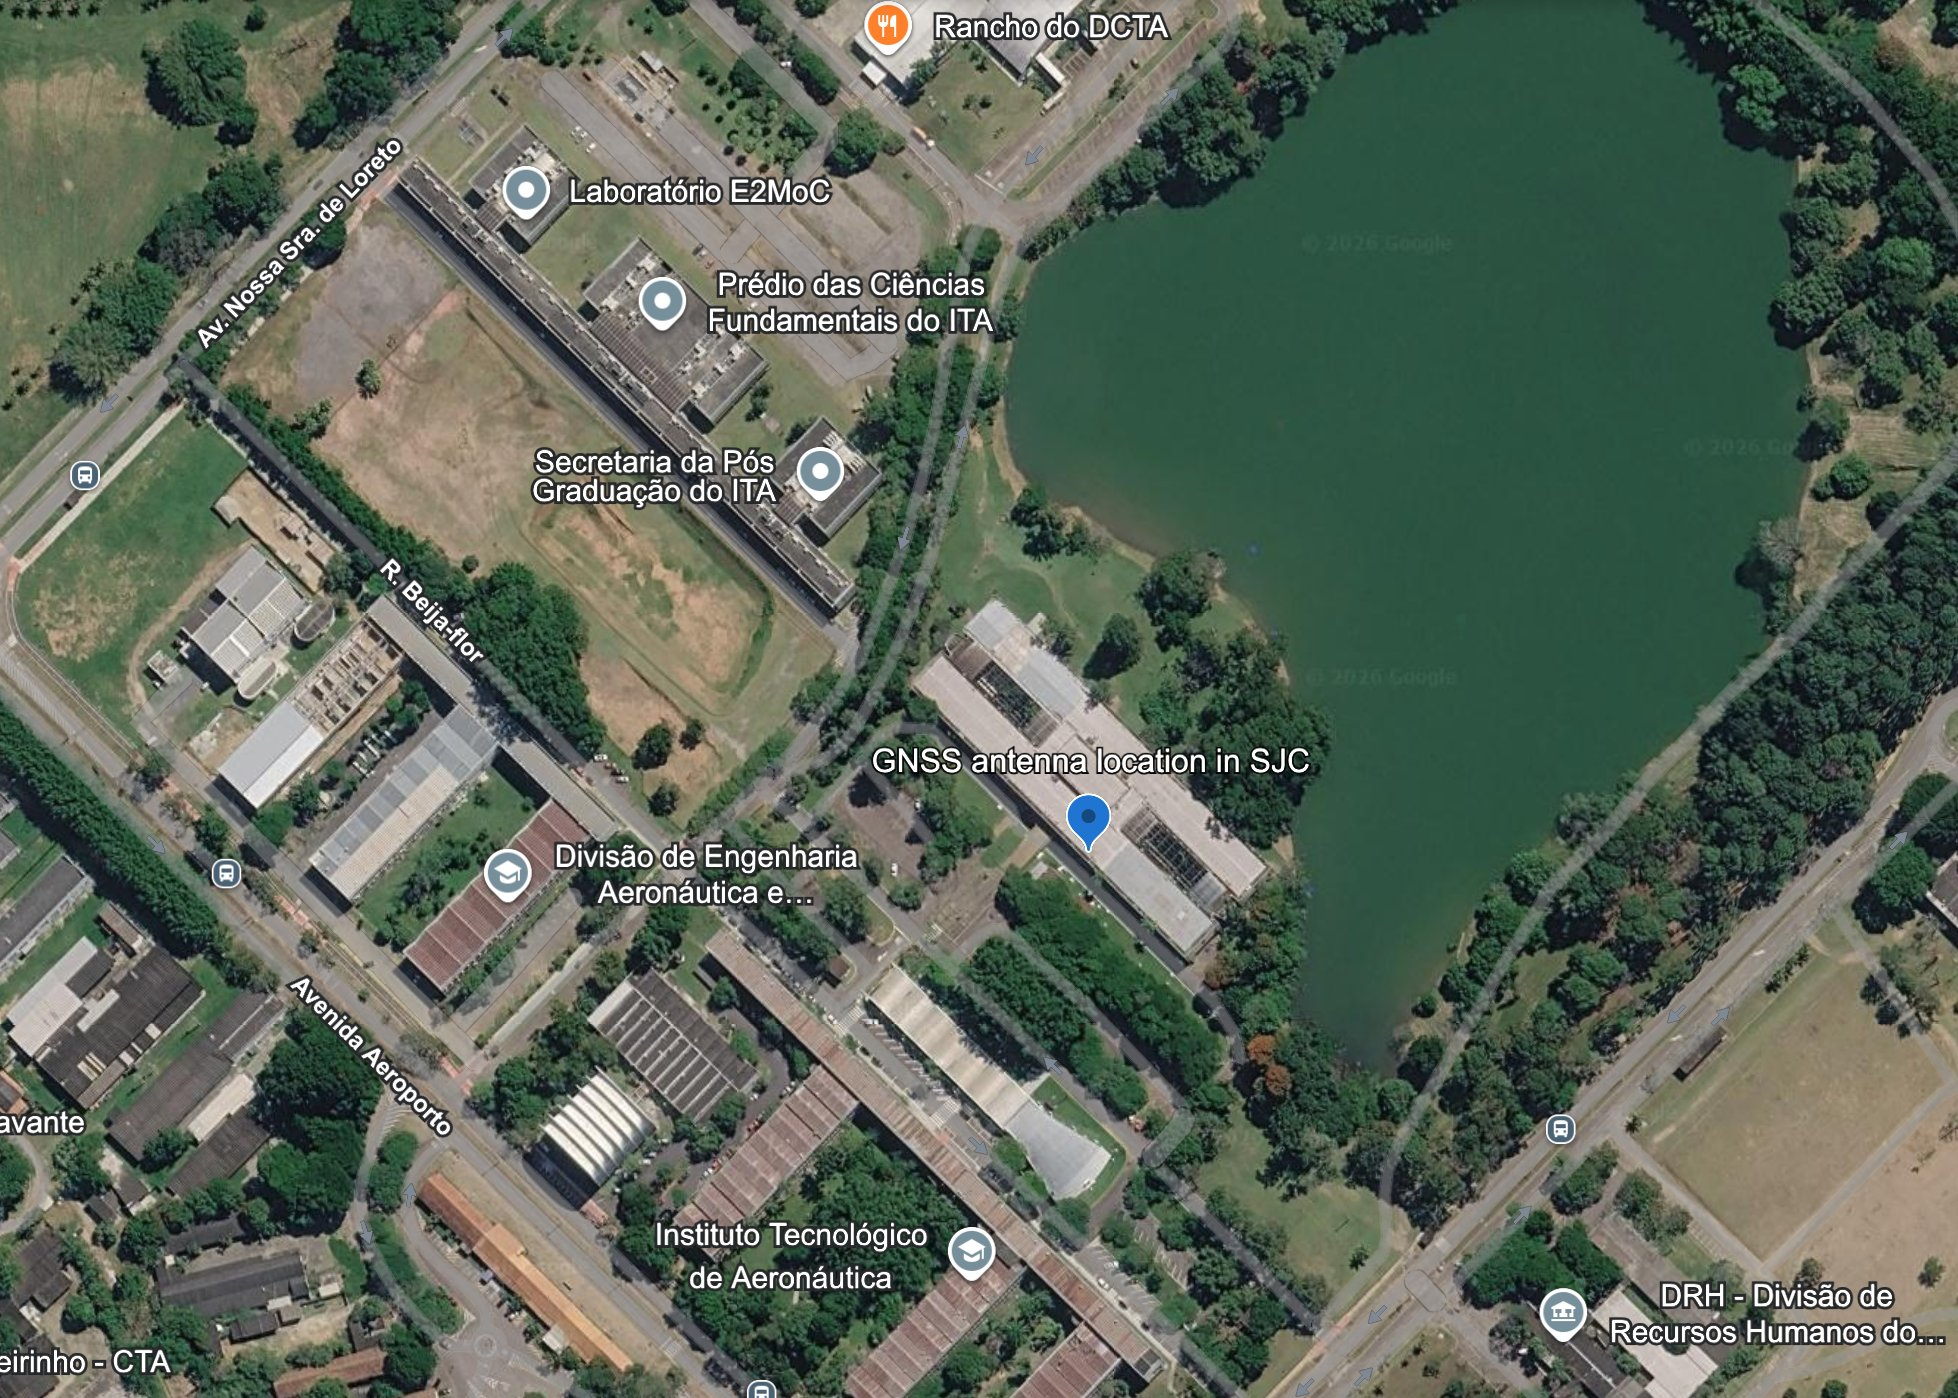
\includegraphics[width=0.65\linewidth]{gnss_antenna_location.jpg}
  \caption{Location of the GNSS antenna.}
  \label{fig:antenna-location}
\end{figure}

\newpage

\tableofcontents

\part{Methodology}
\label{part:data-collection}

This part describes how the data is collected: the recording methodology, which keeps only the recordings that contain ionospheric scintillation, and how each recording is checked with the GNSS-SDR software receiver.

\section{Data collection routine}

The recording is made automatically by a Linux service that follows these guidelines:
\begin{itemize}
    \item Every day, the program starts within the time range [9PM, 11PM] (local time), i.e., the post-sunset hours in which equatorial plasma bubbles cause scintillation at low latitudes.
    \item It senses whether the USRP is detectable via \texttt{uhd\_find\_devices --args=``addr=192.168.10.2''}.
    \item If not found, it exits silently and senses again in intervals of 15 min.
    \item Once found, two recordings are made, each with a duration of 5 minutes (300 s). The first recording (RC0) happens right after the USRP is detected, and the second recording (RC1 ) is made 30 min after the first one. After that, no more recordings are made for that day.
    \item Every recording has two channels (ch0 and ch1), one per GNSS band. The two daily recordings, however, cover distinct band combinations and operate their own sampling rate, as shown in Table~\ref{tab:recording-profiles}. Every channel uses a gain of 25~dB.
    \item RC0 and RC1 are saved as separated SigMF archives. See Section~\ref{sec:sigmf} for details.
    \item Each recording is processed by the GNSS-SDR\footnote{\url{https://gnss-sdr.org}, v0.0.20.} software receiver right after it is made. The final PVT solutions obtained from each recording are listed in Table~\ref{tab:pvt-solutions}.
    \item Before the GNSS-SDR processing, some preprocessing steps described in Section~\ref{sec:preprocessing} are performed.
    \item The recorded data during the last 15 days are kept in NAS's temporary directory, while their respective receiver stage outputs (from acquisition to PVT) are appended to Part~\ref{part:temporary}. From the prompt correlator samples, the scintillation indices are also computed according to Section~\ref{part:scintillation}, and each recording is classified as either weak, moderate or strong scintillation severity.
    \item This report is updated every day and automatically, with the daily recordings moved to the NAS storage and their GNSS-SDR outputs appended to Part~\ref{part:temporary}.
    \item Every 15 days, right after the periodic report update is triggered, the following steps are performed:
    \begin{enumerate}
        \item the report is sent via WhatsApp to the head of the Laboratory, Prof.\ Dr.\ Felix Antreich, together with a summary of the recorded metadata.
        \item the recordings of the past 15 days classified with moderate or strong scintillation are moved to the permanent NAS storage, and only their respective scintillation indices are appended to Part~\ref{part:permanent};
        \item the leftover recordings in NAS's temporary directory is deleted, and Part~\ref{part:temporary} is cleared so that the next 15 days of recordings can be appended to it.
    \end{enumerate}
\end{itemize}

\begin{table}[H]
      \centering
      \caption{Channel configuration of the two daily recordings. The $\rightarrow$ indicates the preprocessing steps made on the recorded data before the GNSS-SDR processing.}
      \label{tab:recording-profiles}
      \small\setlength{\tabcolsep}{4pt}
      \begin{tabular}{|l|c|c|c|c|c|}
        \hline
        \textbf{Recording} & \textbf{Channel}\footnotemark & \textbf{Band} & \textbf{Freq. (MHz)} & \textbf{Rate (MS/s)} & \textbf{I/Q format} \\
        \hline
        First (RC0) & ch0 & L1 & 1575.42 & 4 $\rightarrow$ 20 & 16 $\rightarrow$ 8-bit \\
        \cline{2-6}
         & ch1 & L5 & 1176.45 & 20 & 16 $\rightarrow$ 8-bit \\
        \hline
        Second (RC1) & ch0 & L1 & 1575.42 & 4 & 16-bit \\
        \cline{2-6}
         & ch1 & L2 & 1227.60 & 4 & 16-bit \\
        \hline
      \end{tabular}
    \end{table}
\footnotetext{In the context of the TwinRX daughterboard, ch0 and ch1 are referred to as RX0 and RX1, respectively.}

% landscape page (pdflscape also rotates it in the PDF viewer)
\begin{landscape}
\begin{table}[H]
      \centering
      \caption{Final PVT solutions of each daily recording.}
      \label{tab:pvt-solutions}
      \small
      % Signals and Comments wrap: fixed width for Signals, Comments (X) takes the rest of the line;
      % m columns (and X as m) center every cell vertically in its row
      \renewcommand{\tabularxcolumn}[1]{m{#1}}
      \begin{tabularx}{\linewidth}{|l|c|>{\raggedright\arraybackslash}m{3.2cm}|l|>{\raggedright\arraybackslash}X|}
        \hline
        \textbf{Recording} & \textbf{Solution} & \textbf{Signals} & \textbf{GNSS-SDR configuration file} & \textbf{Comments} \\
        \hline
        First (RC0) & sol0 & GPS L1 C/A (ch0) & \multirow{9}{*}{\texttt{l1ca8bits4msps\_l5\_8bits20msps.conf}} & RC0-ch1 (tuned to L5) is ignored\\
        \cline{2-3}\cline{5-5}
         & sol1 & GPS L1 C/A (ch0) + L5 (ch1) & & Because GNSS-SDR's dual-frequency solver was unstable with few L5-capable GPS satellites in view, this PVT was computed using \texttt{gnss\_spp\_lib.py} from the observables and decoded ephemeris of the GNSS-SDR run. L1 C/A is first upsampled from 4~MS/s to 20~MS/s before being processed by GNSS-SDR. See Section \ref{sec:upsampling} \\
        \cline{2-5}
         & sol2 & Galileo E1-B/C (ch0) + E5a (ch1) & \texttt{e1\_8bits4msps\_e5a\_8bits20msps.conf} & E1-B/C is first upsampled from 4~MS/s to 20~MS/s before being processed by GNSS-SDR. See Section \ref{sec:upsampling} \\
        \hline
        Second (RC1) & sol0 & GPS L1 C/A + Galileo E1-B/C (both from ch0) & \multirow{8}{*}{\texttt{l1ca16bits4msps\_l2c16bits4msps.conf}} & RC1-ch1 (tuned to L2) is ignored\\
        \cline{2-3}\cline{5-5}
         & sol1 & GPS L1 C/A (ch0) + L2C (ch1) & & Since GNSS-SDR\footnotemark{} has no PVT solution using L2C, it was computed by \texttt{gnss\_spp\_lib.py} from the observables and decoded ephemeris of the GNSS-SDR run. \\
        \hline
      \end{tabularx}
\end{table}
\footnotetext{As of GNSS-SDR v0.0.20, the version used in this work.}
\end{landscape}

\begin{note}
For the sake of conciseness, the PVT solutions will be referred to as ``RC0-sol0'', ``RC0-sol1'', ``RC0-sol2'', ``RC1-sol0'' and ``RC1-sol1'' hereafter.
\end{note}

\section{SigMF format}\label{sec:sigmf}

The recordings are stored in the Signal Metadata Format (SigMF)\footnote{\url{https://sigmf.org}.}, an open standard for sharing recorded I/Q samples together with the information needed to interpret them. A SigMF recording consists of two files: a binary \texttt{.sigmf-data} file holding only the raw samples, and a JSON \texttt{.sigmf-meta} file describing them. The metadata is split into a \texttt{global} object (sample format, sampling rate, hardware, checksum, etc.), a \texttt{captures} list (center frequency and start time of each contiguous block of samples), and an \texttt{annotations} list (optional labels over sample ranges). Related recordings, such as the channels of one multichannel acquisition, are grouped by a \texttt{.sigmf-collection} file, and all these files can be bundled into a single \texttt{.sigmf} archive, which is a plain \texttt{tar} file.

Each dual-channel recording is therefore stored as one archive with one recording per channel. For example, the contents of the first recording of 26/10/2026 are listed below:

\begin{codeblock}
tar -tvf recordings/x310_20261026T190001Z.sigmf | numfmt --field=3 --to=iec-i --suffix=B

-rw-r--r-- tapyu/tapyu    572B 2026-10-26 16:05 x310_20261026T190001Z/x310_20261026T190001Z.sigmf-collection
-rw-r--r-- tapyu/tapyu  1.5KiB 2026-10-26 16:05 x310_20261026T190001Z/x310_20261026T190001Z_ch0.sigmf-meta
-rw-r--r-- tapyu/tapyu  2.1KiB 2026-10-26 16:05 x310_20261026T190001Z/x310_20261026T190001Z_ch1.sigmf-meta
-rw-r--r-- tapyu/tapyu  2.3GiB 2026-10-26 16:05 x310_20261026T190001Z/x310_20261026T190001Z_ch0.sigmf-data
-rw-r--r-- tapyu/tapyu   12GiB 2026-10-26 16:05 x310_20261026T190001Z/x310_20261026T190001Z_ch1.sigmf-data
\end{codeblock}

The collection file ties the two channels together, and each channel has its own metadata and data files. The data file sizes follow from the 300-s duration and the channel configuration of Table~\ref{tab:recording-profiles}: channel 0 (L1) holds $4~\text{MS/s} \times 300~\text{s} \times 2~\text{bytes} = 2.4$~GB, and channel 1 (L5) holds $20~\text{MS/s} \times 300~\text{s} \times 2~\text{bytes} = 12$~GB.

\section{Preprocessing steps}\label{sec:preprocessing}

After the recording is made, the following preprocessing steps are performed before the GNSS-SDR processing:

\subsection{Requantization from 16 to 8 bits}

On the one hand, the OTW data format for USRP X310 is sc16, \textit{i.e.}, 16-bit signed integers for each I/Q component, totaling 32 bits (4 byte) per complex baseband sample. On the other hand, the UHD (USRP Hardware Driver) library determines the CPU data format, which is internally handled by the Python's \texttt{uhd} package. However, UHD 4.6 (the one used in the recording) also has no sc16 $\rightarrow$ sc8 converter on the host side. Therefore, it is manually done in \texttt{x310usrp\_record.py} for RC0 (see Table \ref{tab:recording-profiles}).

The requantization is applied right after the USRP recording, so that the stored data file is kept as small as possible.

\subsection{Upsampling for multi-rate channels}
\label{sec:upsampling}

When reading from a file, GNSS-SDR expects all channels to run at the same rate. \texttt{Multichannel\_File\_Signal\_Source} (in the GNSS-SDR's config file) ensures this by reading several raw I/Q files through a single block with one output stream per file. By using the terminal output shown in Section \ref{sec:sigmf} example, they are \texttt{x310\_20261026T190001Z\_ch0.sigmf-data} for ch0 and \texttt{x310\_20261026T190001Z\_ch1.sigmf-data} for ch1. On each call, that block delivers the same number of samples to every stream, so the two bands advance in lockstep\footnote{With one independent source per band, one band runs ahead of the other and its measurements are discarded.}.

When the channels run at the same rate, this procedure is straightforward. However, the data source for RC0-sol1 and sol2 operate at different rates: 4~MS/s for ch0 and 20~MS/s for ch1. Therefore, \texttt{upsample\_iq.py} upsamples via zero-order hold the file \texttt{x310\_20261026T190001Z\_ch0.sigmf-data} to 20~MS/s, generating a new temporary file. Then, the upsampled version of ch0 and \texttt{x310\_20261026T190001Z\_ch1.sigmf-data} is used as input to GNSS-SDR. The upsampling factor is 5, so every sample of ch0 is repeated 5 times in the new file.

The upsampling is done right before the GNSS-SDR processing, generating a temporary file that is deleted right after the processing is finished.

\section{Outputs for the temporary GNSS data}\label{sec:gnss-sdr}

Before looking for scintillation-disturbed data, one must check whether the temporary recordings hold usable GNSS signals. Otherwise, an amplitude or phase fluctuation could come from a faulty recording (\textit{e.g.}, dropped samples, a wrong gain or a missing reference clock) rather than from scintillation. Therefore, RC0-sol0, RC0-sol1, RC0-sol2, RC1-sol0, and RC1-sol1 are all validated at every stage of the GNSS-SDR receiver chain, \textit{i.e.}, signal acquisition and tracking, navigation message decoding, and PVT computation. In addition, the scintillation indices must also be computed, which should be near to zero for nominal operation. In this way, high scintillation indices can be trusted to come from scintillation, rather than a recording problem.

Figure~\ref{fig:gnss-sdr-chain} shows the data chain of GNSS-SDR. Each channel (one per satellite signal) runs its own acquisition, tracking and telemetry decoder; observables and PVT combine all of them.


\begin{figure}[H]
  \centering
  \resizebox{\linewidth}{!}{%
  \begin{tikzpicture}[node distance=0.35cm, every node/.style={font=\scriptsize, align=center},
      block/.style={draw, rounded corners, minimum height=0.9cm, text width=1.45cm, fill=blue!8},
      arrow/.style={-{Latex[length=1.5mm]}}]
    \node[block] (src) {Signal\\source};
    \node[block, below=of src] (cond) {Signal\\conditioner};
    \node[block, below=of cond] (acq) {Acquisition};
    \node[block, right=of acq] (trk) {Tracking};
    \node[block, right=of trk] (tlm) {Telemetry\\decoder};
    \node[block, below=of tlm] (obs) {Observables};
    \node[block, below=of obs] (pvt) {PVT};
    \foreach \a/\b in {src/cond, cond/acq, acq/trk, trk/tlm, tlm/obs, obs/pvt} \draw[arrow] (\a) -- (\b);
    \draw[dashed, rounded corners] ($(acq.north west)+(-0.12,0.25)$) rectangle ($(tlm.south east)+(0.12,-0.25)$);
    \node[right=0.3cm of tlm, text width=2.1cm, align=left] {one channel per satellite signal};
  \end{tikzpicture}}
  \caption{GNSS-SDR receiver chain.}
  \label{fig:gnss-sdr-chain}
\end{figure}

\subsection{Signal source}
Reads the recorded I/Q samples (here, coming from the data files) and delivers them as a stream, one per channel. GNSS-SDR has no output of its own here, so the recording itself is examined.
\begin{itemize}
  \item \textbf{Power spectral density} per channel: the shape of the receiver passband over a flat thermal-noise floor. GNSS signals are 15--20~dB below the noise, so they are invisible here; a narrow peak would be interference.
  \item \textbf{I/Q histograms}: should be Gaussian, centred on zero, and far from the integer limits (no clipping).
  \item \textbf{Table}: format, rate and gain per channel, I/Q standard deviation and mean, percentage of clipped values, and samples lost during the recording (overflows, zero-filled).
\end{itemize}

\subsection{Signal conditioner}
Adapts the input samples (from the binary file) to what the channels process, \textit{i.e.}, converts the file format (signed 8- or 16-bit interleaved I/Q) to complex floating point (data type adapter for C++), optionally filters (input filter) and resamples (resampler).
\begin{itemize}
  \item \textbf{Table} per channel: file format, data type adapter, filter, resampling, and rate before and after.
\end{itemize}

\subsection{Acquisition}
Detects which satellites are present and gives a first, coarse estimate of each one's code delay and Doppler shift, by correlating the signal with the satellite's spreading code over a two-dimensional grid of delays and Doppler frequencies, and comparing the peak with a detection threshold (set by the probability of false alarm). With dual-frequency assistance, the second band (GPS L5 or L2C, Galileo E5a) is only searched for satellites already tracked on L1/E1, around their L1/E1 Doppler scaled to the second frequency. Galileo E1 uses a 4-ms code (BOC(1,1) modulation), so its correlation peak is narrower and has side peaks.
\begin{itemize}
  \item \textbf{Delay--Doppler map} (surface plot) of the strongest detection per band: a single sharp peak well above the floor.
  \item \textbf{Table}: search attempts, detections and detected satellites, and the best test statistic relative to the threshold. Attempts on satellites that are not in view, or that do not broadcast that band (L5 is only on Block IIF and III satellites, L2C on IIR-M, IIF and III), are rejected.
\end{itemize}

\subsection{Tracking}
Follows each detected signal with a delay-lock loop (code) and a phase-lock loop (carrier), producing every 1--20~ms the prompt correlator output (which carries the navigation data bits), the carrier-to-noise density ratio $C/N_0$, the Doppler, the code, and carrier phases.
\begin{itemize}
  \item \textbf{$C/N_0$ and Doppler versus time} per satellite and band: $C/N_0$ of roughly 35--50~dB-Hz for an open-sky antenna, and smooth Doppler curves following the satellite motion.
  \item \textbf{Prompt I/Q scatter} of the strongest satellite per band: with the carrier phase locked, the energy sits on the in-phase axis in two clusters (the $\pm1$ data bits), or in for the dataless pilot components that Galileo is tracked on (E1-C, E5a-Q), the $\pm1$ chips of their secondary code; without phase lock it would be a ring. Each point is one prompt correlator output, the received samples $x[n]$ multiplied by the local code replica $c$ aligned at the estimated code delay $\hat\tau$ and by the local carrier replica (estimated Doppler $\hat f_D$ and phase $\hat\phi$), summed over the $N$ samples of one integration period ($T_s$: sampling period):
  \begin{equation}
    P = \sum_{n=1}^{N} x[n]\,c[n-\hat\tau]\,e^{-j(2\pi \hat f_D n T_s + \hat\phi)} = I + jQ.
  \end{equation}
  \item \textbf{Loop errors versus time} per satellite and band: the PLL carrier-phase error (degrees) and the DLL code-delay error (chips), i.e. the discriminator outputs the loops drive to zero. Noise centred on zero means clean tracking; jumps would mark cycle slips or a loop losing lock.
  \item \textbf{Table} per satellite: median $C/N_0$, percentage of time phase-locked, losses of lock, time tracked, and the standard deviation of the PLL and DLL errors.
\end{itemize}

\subsection{Telemetry decoder}
Synchronizes to the navigation-message bits and frames, checks their parity/CRC (Cyclic Redundancy Check), decodes the ephemeris (orbit and satellite clock), and time-stamps every measurement with the satellite's transmit time (time of week). GPS L1 C/A carries the legacy LNAV message (6-s subframes); L2C and L5 carry CNAV (12-s and 6-s messages). Galileo E1-B carries I/NAV (2-s pages) and E5a-I F/NAV (10-s pages).
\begin{itemize}
  \item \textbf{Timeline} per band and satellite of when a valid transmit time was available.
  \item \textbf{Table}: messages decoded, ephemeris obtained, and when the first valid time of week came.
\end{itemize}

\subsection{Observables}
Aligns all channels on common receiver epochs and forms, for each satellite and band, the pseudorange (from transmit and receive times), the accumulated carrier phase and the Doppler. These are the measurements a positioning algorithm uses; GNSS-SDR also writes them to a RINEX observation file.
\begin{itemize}
  \item \textbf{Availability} of valid pseudoranges per band and satellite over the recording.
  \item \textbf{Second band minus L1/E1 pseudorange} per satellite: the same constant for every satellite (the receiver's inter-band hardware bias) plus the slowly varying, satellite-dependent ionospheric delay difference (metres). It proves that both bands measure the same satellites consistently.
  \item \textbf{Table} per satellite: common epochs, mean, standard deviation and drift of that difference.
\end{itemize}

\subsection{PVT}
Computes position, velocity and receiver clock (PVT) from the pseudoranges and the decoded ephemeris. The antenna position was surveyed: $-23.209433^\circ$, $-45.874875^\circ$, 596.42~m (WGS-84), so the errors below are true errors, not just scatter.
\begin{itemize}
  \item \textbf{Horizontal error scatter and east/north/up error versus time} for GNSS-SDR's own solution of each run and, for the GPS runs, \texttt{gnss\_spp\_lib.py}'s dual-frequency ionosphere-free solution. Single-frequency single-point positioning is expected to stay within a few metres horizontally and ${\sim}10$~m vertically; the iono-free combination removes the ionospheric bias but amplifies the code noise about three times.
  \item \textbf{Sky plot} of the GPS satellites used by \texttt{gnss\_spp\_lib.py}.
  \item \textbf{Table}: mean error (accuracy), standard deviation (precision), 2-D and 3-D RMS, and 95\% horizontal error.
\end{itemize}

\newpage

\part{Scintillation index computation}
\label{part:scintillation}

This part introduces the signal model assumed for the recorded data and the procedure to compute the amplitude ($S_4$) and phase ($\sigma_\phi$) scintillation indices from the correlator outputs of the software receiver, following \cite{wendlerScintillationProcessingSoftware2016,vandierendonckIonosphericScintillationMonitoring1993,vandierendonckMeasuringIonosphericScintillation2004}. It ends with the three scintillation severity classes that decide which recordings are stored permanently.

\section{Signal model}
\label{sec:signal-model}

The signals of the $K$ satellites in view on the carrier frequencies $f_{\mathrm{c},l}$, $l = 1, \ldots, L$, are well separated by their spreading codes and frequencies. Therefore, it is sufficient to consider the signal of the $k$th satellite on the $l$th carrier on its own \cite{wendlerScintillationProcessingSoftware2016}:
\begin{equation}
  y_{\mathrm{RF},kl}(t) = A_{kl}(t)\, c_{kl}\big(t - \tau_{kl}(t)\big)\, d_{kl}\big(t - \tau_{kl}(t)\big) \operatorname{cos}\big(2\pi f_{\mathrm{c},l}\, t + \phi_{kl}(t)\big) + \eta(t),
\end{equation}
where $A_{kl}(t)$ is the signal amplitude, $c_{kl}(t)$ and $d_{kl}(t)$ are the spreading code and navigation data, $\tau_{kl}(t)$ is the signal delay, $\phi_{kl}(t)$ is the carrier phase (which includes the Doppler shift), and $\eta(t)$ is zero-mean white Gaussian noise. The TwinRX daughterboards of the X310 filter and down-convert each band directly to baseband and sample it at $f_s = 1/T_s$, so that each channel of a recording holds the complex baseband samples (subscripts $k$, $l$ omitted from now on)
\begin{equation}
  \label{eq:baseband-signal}
  y[n] = A[n]\, e^{j\phi[n]}\, c(nT_s - \tau[n])\, d(nT_s - \tau[n]) + \eta[n] = y_\mathrm{I}[n] + j y_\mathrm{Q}[n],
\end{equation}
with the short notations $A[n] = A(nT_s)$, $\tau[n] = \tau(nT_s)$, $\phi[n] = \phi(nT_s)$. The phase $\phi[n]$ also holds the instabilities of the X310's local oscillator, which is disciplined by an external 10~MHz reference. Ionospheric scintillation shows up as fast fluctuations of the amplitude $A[n]$ (amplitude scintillation) and of the phase $\phi[n]$ (phase scintillation).

\paragraph{Phase and delay model.} The carrier phase and the signal delay can be decomposed into \cite{wendlerScintillationProcessingSoftware2016}
\begin{align}
  \phi(t) &= \frac{2\pi}{\lambda_\mathrm{c}} \Big( r(t) + c\big(\tau^{\mathrm{clk,s}}(t) - \tau^{\mathrm{clk,r}}(t)\big) + \tau^{\mathrm{tro}}(t) - \tau^{\mathrm{ion}}(t) \Big) + \eta^\phi, \\
  \tau(t) &= \frac{1}{c} \Big( r(t) + c\big(\tau^{\mathrm{clk,s}}(t) - \tau^{\mathrm{clk,r}}(t)\big) + \tau^{\mathrm{tro}}(t) + \tau^{\mathrm{ion}}(t) \Big) + \eta^\tau,
\end{align}
where $\lambda_\mathrm{c} = c/f_\mathrm{c}$, $c$ is the speed of light, $r(t)$ is the line-of-sight distance from the satellite to the receiver, $\tau^{\mathrm{clk,s}}(t)$ and $\tau^{\mathrm{clk,r}}(t)$ are the satellite and receiver clock offsets, $\tau^{\mathrm{tro}}(t)$ and $\tau^{\mathrm{ion}}(t)$ are the tropospheric and ionospheric delays, and $\eta^\phi$, $\eta^\tau$ are higher-order noise processes. The ionosphere advances the phase and delays the code, hence the opposite signs. To isolate the scintillation, the slow terms (geometry, clocks, troposphere and the mean ionospheric delay) must be removed: this is the purpose of the detrending steps below.

\section{Correlator outputs}
\label{sec:correlator-outputs}

The tracking loops of the receiver (Section~\ref{sec:gnss-sdr}) wipe off the carrier with their numerically controlled oscillator (NCO) and correlate the result with a local code replica, over a coherent integration time $T_\mathrm{coh} = M_s T_s$ of $M_s$ samples. The $m$th prompt correlator output reads \cite{wendlerScintillationProcessingSoftware2016}
\begin{align}
  I[m] &= \frac{M_s \bar A[m]\, d[m]}{2} R_c(\tau_\mathrm{e}[m]) \operatorname{cos}\big(2\pi f_\mathrm{e}[m]\, m T_\mathrm{coh} + \phi_\mathrm{e}[m]\big) + \eta_{c,\mathrm{I}}[m], \label{eq:prompt-i}\\
  Q[m] &= \frac{M_s \bar A[m]\, d[m]}{2} R_c(\tau_\mathrm{e}[m]) \operatorname{sin}\big(2\pi f_\mathrm{e}[m]\, m T_\mathrm{coh} + \phi_\mathrm{e}[m]\big) + \eta_{c,\mathrm{Q}}[m], \label{eq:prompt-q}
\end{align}
where $\bar A[m]$ is the mean amplitude within the integration interval, $d[m] \in \{-1, 1\}$ is the data symbol, $R_c(\cdot)$ is the code autocorrelation function, $\tau_\mathrm{e}[m]$, $f_\mathrm{e}[m]$ and $\phi_\mathrm{e}[m]$ are the code-delay, frequency and phase errors of the loops, and $\eta_{c,\mathrm{I}}[m]$, $\eta_{c,\mathrm{Q}}[m]$ are zero-mean Gaussian noises of variance $\sigma_n^2/2$ each, with $\sigma_n^2 = N_0/T_\mathrm{coh}$. These are the prompt I/Q outputs dumped by GNSS-SDR's tracking. GNSS-SDR integrates over 1~ms during pull-in and over up to 20~ms once bit-synchronized (10~ms for the L5 and E5a pilots). The scintillation indices are computed from $M$ consecutive outputs such that $M\,T_\mathrm{coh} = 20$~ms, i.e., a 50~Hz signal intensity that never straddles a GPS L1 C/A data-bit transition \cite{lopesLinearTimeinvariantFiltering2023}.

\section{Amplitude scintillation index \texorpdfstring{$S_4$}{S4}}
\label{sec:s4}

The amplitude scintillation index is the standard deviation of the signal intensity normalized by its mean \cite{briggsVariationRadioStar1963}:
\begin{equation}
  \label{eq:s4-definition}
  S_4 = \sqrt{\frac{\mathrm{E}\big(\rho^2[b]\big) - \mathrm{E}\big(\rho[b]\big)^2}{\mathrm{E}\big(\rho[b]\big)^2}},
\end{equation}
where $\rho[b]$ is the signal intensity of the $b$th 20-ms interval and $\mathrm{E}(\cdot)$ is the expectation, replaced, under ergodicity, by the time average over 60~s.

\paragraph{Signal intensity.} Under scintillation, the loop errors are not negligible and the signal energy spreads over $I$ and $Q$, so both are used. The narrow-band and wide-band powers of the $b$th interval are \cite{vandierendonckIonosphericScintillationMonitoring1993,wendlerScintillationProcessingSoftware2016}
\begin{equation}
  P[b] = \Big(\sum_{m=1}^{M} I[m]\Big)^2 + \Big(\sum_{m=1}^{M} Q[m]\Big)^2, \qquad
  \tilde P[b] = \sum_{m=1}^{M} \big(I^2[m] + Q^2[m]\big),
\end{equation}
and their difference $\rho[b] = P[b] - \tilde P[b]$ is the raw signal intensity, whose expectation is proportional to $\bar A^2[b]$, without the noise-power offset that $\tilde P[b]$ alone would carry.

\paragraph{Detrending.} The intensity also varies because of the satellite motion (antenna gain, path loss) and multipath, which are not scintillation. Therefore, $\rho[b]$ is filtered by a sixth-order Butterworth low-pass filter $h[b]$ with a 0.1~Hz cut-off frequency, and normalized by the result \cite{vandierendonckIonosphericScintillationMonitoring1993}:
\begin{equation}
  \bar\rho[b] = h[b] * \rho[b], \qquad \rho_\mathrm{det}[b] = \frac{\rho[b]}{\bar\rho[b]}.
\end{equation}
$\rho_\mathrm{det}[b]$ replaces $\rho[b]$ in the $S_4$ estimate below.

\paragraph{Ambient noise removal.} Even with a constant amplitude, the noise makes the estimated intensity fluctuate, which biases $S_4$ upwards. For a constant amplitude, this noise-induced index is \cite{wendlerScintillationProcessingSoftware2016}
\begin{equation}
  S_{4,N_0} = \sqrt{\frac{2}{M T_\mathrm{coh}\, C/N_0} \left(1 + \frac{1}{2(M-1)\, T_\mathrm{coh}\, C/N_0}\right)},
\end{equation}
with $C/N_0$ in linear units (Hz). For $T_\mathrm{coh} = 1$~ms and $M = 20$, it reduces to the well-known $S_{4,N_0}^2 = \frac{100}{C/N_0}\left(1 + \frac{500}{19\, C/N_0}\right)$ \cite{vandierendonckIonosphericScintillationMonitoring1993}. The corrected index, using the 60-s average of the $C/N_0$ estimated by the tracking loops, is
\begin{equation}
  \label{eq:s4-corrected}
  S_4 = \sqrt{\frac{\mathrm{E}\big(\rho_\mathrm{det}^2[b]\big) - \mathrm{E}\big(\rho_\mathrm{det}[b]\big)^2}{\mathrm{E}\big(\rho_\mathrm{det}[b]\big)^2} - \frac{2}{M T_\mathrm{coh}\, C/N_0} \left(1 + \frac{1}{2(M-1)\, T_\mathrm{coh}\, C/N_0}\right)},
\end{equation}
set to zero when the radicand is negative (no scintillation at all). One value is computed every 60~s per satellite and band, i.e., five per satellite and band in a 5-min recording.

\section{Phase scintillation index \texorpdfstring{$\sigma_\phi$}{sigma-phi}}
\label{sec:sigma-phi}

The phase scintillation index is the standard deviation of the detrended carrier phase, over 60~s \cite{vandierendonckMeasuringIonosphericScintillation2004}:
\begin{equation}
  \sigma_\phi = \sqrt{\mathrm{E}\big(\phi^2\big) - \mathrm{E}\big(\phi\big)^2}.
\end{equation}
The phase measured by the $i$th tracking channel holds, besides the scintillation phase $\phi_{\mathrm{sci},i}$, the phase due to the satellite motion $\phi_{\mathrm{sat},i}$, the oscillator instability $\phi_\mathrm{clk}$ (common to all channels), and white noise $\eta_{\phi,i}$ \cite{wendlerScintillationProcessingSoftware2016}:
\begin{equation}
  \phi_{\mathrm{e},i} = \phi_{\mathrm{sat},i} + \phi_\mathrm{clk} + \phi_{\mathrm{sci},i} + \eta_{\phi,i}.
\end{equation}
These terms are removed in three steps \cite{wendlerScintillationProcessingSoftware2016}:
\begin{enumerate}
  \item \textbf{Clock error removal.} The oscillator phase noise is not removed by filtering and would dominate $\sigma_\phi$, which is why scintillation monitors use oven-controlled oscillators \cite{vandierendonckIonosphericScintillationMonitoring1993}. Since $\phi_\mathrm{clk}$ is common to all channels, it cancels in the difference to a reference channel whose satellite shows no phase scintillation (e.g., the highest one):
  \begin{equation}
    \phi_{\mathrm{e},i\text{-ref}} = \phi_{\mathrm{e},i} - \phi_{\mathrm{e,ref}} = \phi_{\mathrm{sat},i} - \phi_{\mathrm{sat,ref}} + \phi_{\mathrm{sci},i} + \eta_{\phi,i} - \eta_{\phi,\mathrm{ref}}.
  \end{equation}
  \item \textbf{Geometry error removal.} For a static receiver, $\phi_{\mathrm{sat},i} - \phi_{\mathrm{sat,ref}}$ is well modelled by a third-order polynomial over a few minutes. Subtracting a third-order polynomial fit leaves $\phi_{\mathrm{det},i} \approx \phi_{\mathrm{sci},i} + \eta_{\phi,i} - \eta_{\phi,\mathrm{ref}}$.
  \item \textbf{Low-frequency component removal.} The remaining slow variations, which are not due to scintillation, are removed by a sixth-order Butterworth high-pass filter (a cascade of three second-order sections) with a 0.1~Hz cut-off frequency, and $\sigma_\phi$ is computed from its output.
\end{enumerate}

\section{Scintillation severity classes and storage}
\label{sec:scintillation-classes}

The scintillation indices are compared with preset thresholds, which are empirical and vary with the application \cite{vandierendonckMeasuringIonosphericScintillation2004,jiaoComparisonEffectHighlatitude2015}. Following the usual amplitude-based detection, every 60-s $S_4$ value is assigned to one of the three severity classes of Table~\ref{tab:scintillation-classes} \cite{jiaoComparisonEffectHighlatitude2015}. To exclude multipath and noisy measurements, only satellites above a $30^\circ$ elevation mask with $C/N_0 \geq 37$~dB-Hz are considered, and the index must stay within the class thresholds for at least 30~s. A recording takes the highest class reached by any of its satellites and bands. $\sigma_\phi$ is reported alongside $S_4$, but it does not decide the class, since it depends on the stability of the receiver's oscillator.

\begin{table}[H]
  \centering
  \begin{tabular}{|l|c|l|}
    \hline
    \textbf{Class} & \textbf{$S_4$ (60 s)} & \textbf{Storage of the recording} \\
    \hline
    No (or weak) scintillation & $S_4 \leq 0.2$ & deleted after the 15-day cycle \\
    \hline
    Moderate scintillation & $0.2 < S_4 \leq 0.5$ & permanent storage (Part~\ref{part:permanent}) \\
    \hline
    Strong scintillation & $S_4 > 0.5$ & permanent storage (Part~\ref{part:permanent}) \\
    \hline
  \end{tabular}
  \caption{Scintillation severity classes and what is done with each recording at the end of its 15-day cycle.}
  \label{tab:scintillation-classes}
\end{table}

Thus, only the recordings with moderate or strong scintillation are kept: they are moved to the permanent storage, while the recordings with no scintillation are deleted (Methodology, Part~\ref{part:data-collection}).

\newpage

\part{Temporary GNSS data}
\label{part:temporary}

This part holds the recordings of the last 15 recording days (days with at least one recording), with all the outputs derived from them so far. This data is temporary: at the end of each 15-day cycle, only the recordings with moderate or strong scintillation (Section~\ref{sec:scintillation-classes}) are moved to the permanent storage (Part~\ref{part:permanent}), the others are deleted, and this part is overwritten with the new 15 days. Older days are kept in the repository history.

Table~\ref{tab:temporary-calendar} shows the days of this 15-day window when recordings were made. The color of each day indicates how many recordings were made on that day: \textcolor{green}{green} means 2 recordings, \textcolor{blue}{blue} means 1 recording, and no color means no recording was made.

\begin{table}[H]
  \centering
  \begin{tabular}{ccc}
    \begin{tikzpicture}[day xshift=3ex, day yshift=3ex]
    % month title and weekday-initials header, placed manually (one calendar
    % "row" apart each) since the built-in month label collides with a header row
    \calendar[dates=2026-10-01 to 2026-10-last,
        week list,
        month label above centered,
        day xshift = 0.6cm,
        day headings=orange,
        day letter headings,
        execute before day scope={%
          \ifdate{equals=2026-10-08}{%
            \tikzset{every day/.append style={fill=blue!40, text=blue, shape=rectangle, inner sep=2pt}}%
          }{}%
          \ifdate{equals=2026-10-13}{%
            \tikzset{every day/.append style={fill=green!40, text=blue, shape=rectangle, inner sep=2pt}}%
          }{}%
          \ifdate{equals=2026-10-14}{%
            \tikzset{every day/.append style={fill=green!40, text=blue, shape=rectangle, inner sep=2pt}}%
          }{}%
          \ifdate{equals=2026-10-15}{%
            \tikzset{every day/.append style={fill=green!40, text=blue, shape=rectangle, inner sep=2pt}}%
          }{}%
          \ifdate{equals=2026-10-16}{%
            \tikzset{every day/.append style={fill=green!40, text=blue, shape=rectangle, inner sep=2pt}}%
          }{}%
          \ifdate{equals=2026-10-19}{%
            \tikzset{every day/.append style={fill=green!40, text=blue, shape=rectangle, inner sep=2pt}}%
          }{}%
          \ifdate{equals=2026-10-20}{%
            \tikzset{every day/.append style={fill=green!40, text=blue, shape=rectangle, inner sep=2pt}}%
          }{}%
          \ifdate{equals=2026-10-21}{%
            \tikzset{every day/.append style={fill=green!40, text=blue, shape=rectangle, inner sep=2pt}}%
          }{}%
          \ifdate{equals=2026-10-22}{%
            \tikzset{every day/.append style={fill=green!40, text=blue, shape=rectangle, inner sep=2pt}}%
          }{}%
          \ifdate{equals=2026-10-23}{%
            \tikzset{every day/.append style={fill=green!40, text=blue, shape=rectangle, inner sep=2pt}}%
          }{}%
          \ifdate{equals=2026-10-24}{%
            \tikzset{every day/.append style={fill=green!40, text=blue, shape=rectangle, inner sep=2pt}}%
          }{}%
          \ifdate{equals=2026-10-25}{%
            \tikzset{every day/.append style={fill=green!40, text=blue, shape=rectangle, inner sep=2pt}}%
          }{}%
          \ifdate{equals=2026-10-26}{%
            \tikzset{every day/.append style={fill=green!40, text=blue, shape=rectangle, inner sep=2pt}}%
          }{}%
        },
        execute after day scope={%
          \ifdate{equals=2026-10-08}{%
            \tikzset{every day/.style={anchor=base east}}%
          }{}%
          \ifdate{equals=2026-10-13}{%
            \tikzset{every day/.style={anchor=base east}}%
          }{}%
          \ifdate{equals=2026-10-14}{%
            \tikzset{every day/.style={anchor=base east}}%
          }{}%
          \ifdate{equals=2026-10-15}{%
            \tikzset{every day/.style={anchor=base east}}%
          }{}%
          \ifdate{equals=2026-10-16}{%
            \tikzset{every day/.style={anchor=base east}}%
          }{}%
          \ifdate{equals=2026-10-19}{%
            \tikzset{every day/.style={anchor=base east}}%
          }{}%
          \ifdate{equals=2026-10-20}{%
            \tikzset{every day/.style={anchor=base east}}%
          }{}%
          \ifdate{equals=2026-10-21}{%
            \tikzset{every day/.style={anchor=base east}}%
          }{}%
          \ifdate{equals=2026-10-22}{%
            \tikzset{every day/.style={anchor=base east}}%
          }{}%
          \ifdate{equals=2026-10-23}{%
            \tikzset{every day/.style={anchor=base east}}%
          }{}%
          \ifdate{equals=2026-10-24}{%
            \tikzset{every day/.style={anchor=base east}}%
          }{}%
          \ifdate{equals=2026-10-25}{%
            \tikzset{every day/.style={anchor=base east}}%
          }{}%
          \ifdate{equals=2026-10-26}{%
            \tikzset{every day/.style={anchor=base east}}%
          }{}%
        }]
        ;
    %   if (Sunday) [red]
    %   if (Saturday) [red];
  \end{tikzpicture}
  &
  % PLACEHOLDER
  &
  % PLACEHOLDER
  \\[2ex]
  \end{tabular}
  \caption{Temporary recording calendar.}
  \label{tab:temporary-calendar}
\end{table}

\section{Records on 08/10/2026}

\subsection{First record}
\begin{table}[H]
  \centering
  \begin{tabular}{|l|l|l|}
    \hline
    \textbf{Parameter} & \textbf{Channel 0} & \textbf{Channel 1} \\
    \hline
    Start time & \multicolumn{2}{>{\centering\arraybackslash}p{7cm}|}{2026-10-08 22:26:37 UTC} \\
    \hline
    Frequency & 1575.420 MHz (L1) & 1176.450 MHz (L5) \\
    \hline
    Duration & \multicolumn{2}{>{\centering\arraybackslash}p{7cm}|}{300.0 s} \\
    \hline
    Sample rate & \multicolumn{2}{>{\centering\arraybackslash}p{7cm}|}{2.000 MS/s} \\
    \hline
    Sample type & \multicolumn{2}{>{\centering\arraybackslash}p{7cm}|}{signed complex 16-bit samples (I+Q), little-endian} \\
    \hline
    Gain & 20.0 dB & 20.0 dB \\
    \hline
    Antenna & RX1 & RX2 \\
    \hline
    File size & 2400.0 MB & 2400.0 MB \\
    \hline
    Samples written & 600,000,000 & 600,000,000 \\
    \hline
    Lost samples & 0 & 0 \\
    \hline
    Clock source & \multicolumn{2}{>{\centering\arraybackslash}p{7cm}|}{external} \\
    \hline
    Time source & \multicolumn{2}{>{\centering\arraybackslash}p{7cm}|}{internal} \\
    \hline
    Motherboard & \multicolumn{2}{>{\centering\arraybackslash}p{7cm}|}{USRP X310} \\
    \hline
    Daughterboard & TwinRX RX0 & TwinRX RX1 \\
    \hline
    Recorder & \multicolumn{2}{>{\centering\arraybackslash}p{7cm}|}{UHD Python API} \\
    \hline
  \end{tabular}
  \caption{Metadata for recording \texttt{x310\_20261008T222630Z}, captured starting 2026-10-08T22:26:37.215640Z.}
\end{table}

\section{Records on 13/10/2026}

\subsection{First record}
\begin{table}[H]
  \centering
  \begin{tabular}{|l|l|l|}
    \hline
    \textbf{Parameter} & \textbf{Channel 0} & \textbf{Channel 1} \\
    \hline
    Start time & \multicolumn{2}{>{\centering\arraybackslash}p{7cm}|}{2026-10-13 21:57:56 UTC} \\
    \hline
    Frequency & 1575.420 MHz (L1) & 1176.450 MHz (L5) \\
    \hline
    Duration & \multicolumn{2}{>{\centering\arraybackslash}p{7cm}|}{300.0 s} \\
    \hline
    Sample rate & \multicolumn{2}{>{\centering\arraybackslash}p{7cm}|}{2.000 MS/s} \\
    \hline
    Sample type & \multicolumn{2}{>{\centering\arraybackslash}p{7cm}|}{signed complex 16-bit samples (I+Q), little-endian} \\
    \hline
    Gain & 20.0 dB & 20.0 dB \\
    \hline
    Antenna & RX1 & RX2 \\
    \hline
    File size & 2400.0 MB & 2400.0 MB \\
    \hline
    Samples written & 600,000,000 & 600,000,000 \\
    \hline
    Lost samples & 0 & 0 \\
    \hline
    Clock source & \multicolumn{2}{>{\centering\arraybackslash}p{7cm}|}{external} \\
    \hline
    Time source & \multicolumn{2}{>{\centering\arraybackslash}p{7cm}|}{internal} \\
    \hline
    Motherboard & \multicolumn{2}{>{\centering\arraybackslash}p{7cm}|}{USRP X310} \\
    \hline
    Daughterboard & TwinRX RX0 & TwinRX RX1 \\
    \hline
    Recorder & \multicolumn{2}{>{\centering\arraybackslash}p{7cm}|}{UHD Python API} \\
    \hline
  \end{tabular}
  \caption{Metadata for recording \texttt{x310\_20261013T215749Z}, captured starting 2026-10-13T21:57:56.746726Z.}
\end{table}

\subsection{Second record}
\begin{table}[H]
  \centering
  \begin{tabular}{|l|l|l|}
    \hline
    \textbf{Parameter} & \textbf{Channel 0} & \textbf{Channel 1} \\
    \hline
    Start time & \multicolumn{2}{>{\centering\arraybackslash}p{7cm}|}{2026-10-13 22:08:41 UTC} \\
    \hline
    Frequency & 1575.420 MHz (L1) & 1176.450 MHz (L5) \\
    \hline
    Duration & \multicolumn{2}{>{\centering\arraybackslash}p{7cm}|}{300.0 s} \\
    \hline
    Sample rate & \multicolumn{2}{>{\centering\arraybackslash}p{7cm}|}{2.000 MS/s} \\
    \hline
    Sample type & \multicolumn{2}{>{\centering\arraybackslash}p{7cm}|}{signed complex 16-bit samples (I+Q), little-endian} \\
    \hline
    Gain & 20.0 dB & 20.0 dB \\
    \hline
    Antenna & RX1 & RX2 \\
    \hline
    File size & 2400.0 MB & 2400.0 MB \\
    \hline
    Samples written & 600,000,000 & 600,000,000 \\
    \hline
    Lost samples & 0 & 0 \\
    \hline
    Clock source & \multicolumn{2}{>{\centering\arraybackslash}p{7cm}|}{external} \\
    \hline
    Time source & \multicolumn{2}{>{\centering\arraybackslash}p{7cm}|}{internal} \\
    \hline
    Motherboard & \multicolumn{2}{>{\centering\arraybackslash}p{7cm}|}{USRP X310} \\
    \hline
    Daughterboard & TwinRX RX0 & TwinRX RX1 \\
    \hline
    Recorder & \multicolumn{2}{>{\centering\arraybackslash}p{7cm}|}{UHD Python API} \\
    \hline
  \end{tabular}
  \caption{Metadata for recording \texttt{x310\_20261013T220835Z}, captured starting 2026-10-13T22:08:41.589855Z.}
\end{table}


\section{Records on 22/10/2026}

\subsection{First record}
\begin{table}[H]
  \centering
  \begin{tabular}{|l|l|l|}
    \hline
    \textbf{Parameter} & \textbf{Channel 0} & \textbf{Channel 1} \\
    \hline
    Start time & \multicolumn{2}{>{\centering\arraybackslash}p{7cm}|}{2026-10-22 19:00:06 UTC} \\
    \hline
    Frequency & 1575.420 MHz (L1) & 1176.450 MHz (L5) \\
    \hline
    Duration & 300.0 s & 300.0 s \\
    \hline
    Sample rate & 4.000 MS/s & 20.000 MS/s \\
    \hline
    Sample type & \multicolumn{2}{>{\centering\arraybackslash}p{7cm}|}{signed complex 8-bit samples (I+Q), converted on the host from the X310's sc16} \\
    \hline
    Gain & 25.0 dB & 25.0 dB \\
    \hline
    Antenna & RX1 & RX2 \\
    \hline
    File size & 2400.0 MB & 12000.0 MB \\
    \hline
    Samples written & 1,200,000,000 & 6,000,000,000 \\
    \hline
    Lost samples & 2912 & 14924 \\
    \hline
    Clock source & \multicolumn{2}{>{\centering\arraybackslash}p{7cm}|}{external} \\
    \hline
    Time source & \multicolumn{2}{>{\centering\arraybackslash}p{7cm}|}{internal} \\
    \hline
    Motherboard & \multicolumn{2}{>{\centering\arraybackslash}p{7cm}|}{USRP X310} \\
    \hline
    Daughterboard & TwinRX RX0 & TwinRX RX1 \\
    \hline
    Recorder & \multicolumn{2}{>{\centering\arraybackslash}p{7cm}|}{UHD Python API} \\
    \hline
    GNSS-SDR configuration & \multicolumn{2}{>{\centering\arraybackslash}p{7cm}|}{\texttt{l1ca8bits4msps\_l5\_8bits20msps.conf}, \texttt{e1\_8bits4msps\_e5a\_8bits20msps.conf}} \\
    \hline
  \end{tabular}
  \caption{Metadata for recording \texttt{x310\_20261022T190000Z}, captured starting 2026-10-22T19:00:06.973177Z.}
\end{table}

\subsubsection{Signal source}
Raw I/Q samples of each channel, as recorded (0.5~s analysed, from 10~s into the recording).

\begin{figure}[H]
  \centering
  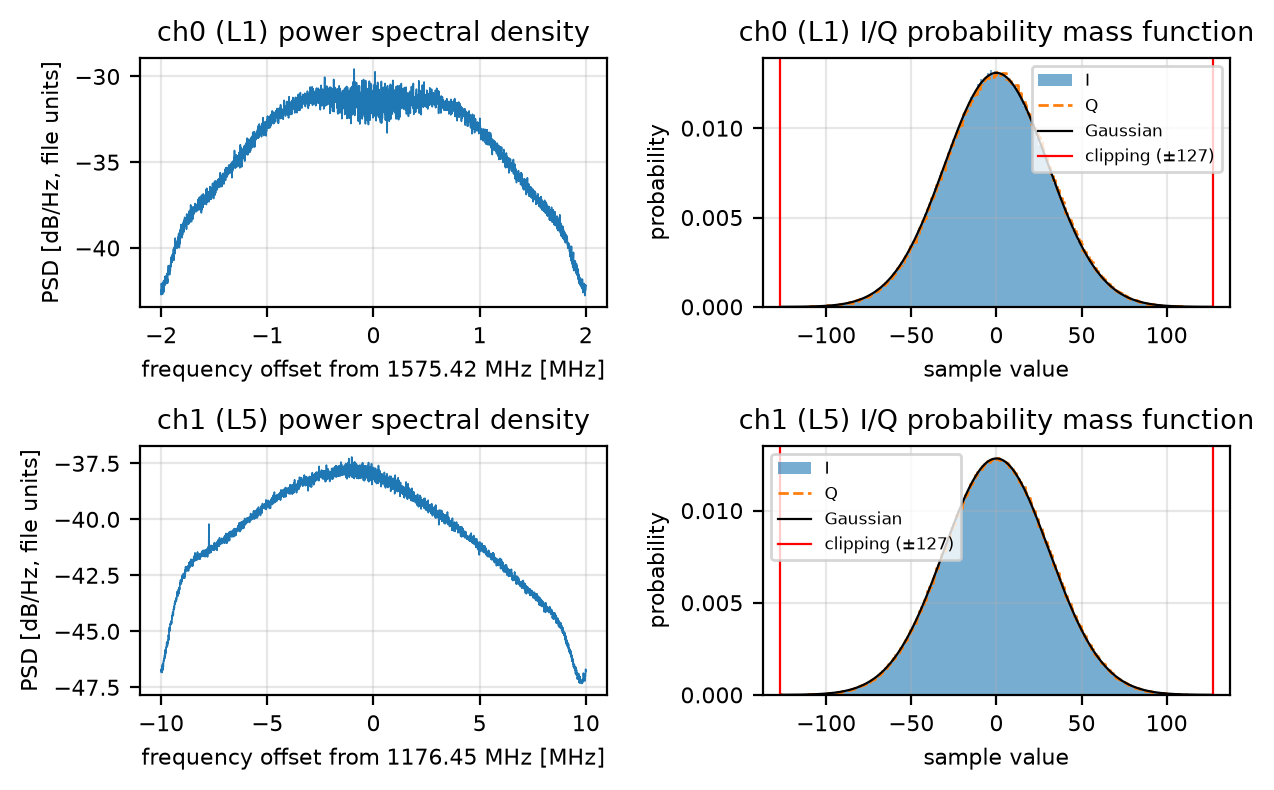
\includegraphics[width=1.0\linewidth]{gnss_sdr/x310_20261022T190000Z/source.png}
  \caption{Signal source: power spectral density (the receiver passband over a flat thermal-noise floor; GNSS signals are below the noise, so only interference would stand out) and I/Q histograms (Gaussian noise, centred, not clipped).}
\end{figure}

\begin{table}[H]
  \centering
  \footnotesize
  \resizebox{\ifdim\width>\linewidth\linewidth\else\width\fi}{!}{%
  \begin{tabular}{lcc}
    \hline
    \textbf{Channel} & \textbf{ch0} & \textbf{ch1} \\
    \hline
    Frequency [MHz] & 1575.42 & 1176.45 \\
    Rate [MS/s] & 4 & 20 \\
    Format & ci8 & ci8 \\
    Gain [dB] & 25 & 25 \\
    Std I / Q & 30.4 / 30.5 & 31.1 / 31.1 \\
    Mean I / Q & -0.26 / 0.20 & 0.26 / -0.07 \\
    Clipped [\%] & 0.003 & 0.004 \\
    Lost samples & 2,912 & 14,924 \\
    \hline
  \end{tabular}}
  \caption{Signal source: sample statistics per channel.}
\end{table}

\subsubsection{Signal conditioner}
How each recorded channel is turned into the complex baseband stream the channels process.

\begin{table}[H]
  \centering
  \footnotesize
  \resizebox{\ifdim\width>\linewidth\linewidth\else\width\fi}{!}{%
  \begin{tabular}{lcc}
    \hline
    \textbf{Channel} & \textbf{ch0 (L1 C/A)} & \textbf{ch1 (L5)} \\
    \hline
    File format & ci8 & ci8 \\
    Source item type & ibyte & ibyte \\
    Data type adapter & Ibyte\_To\_Complex & Ibyte\_To\_Complex \\
    Input filter & Pass\_Through & Pass\_Through \\
    Resampling & \$\textbackslash{}times\$5 zero-order hold (offline) & Pass\_Through \\
    Rate [MS/s] & 4 $\to$ 20 & 20 $\to$ 20 \\
    \hline
  \end{tabular}}
  \caption{Signal conditioner: recorded format and rate to gnss-sdr's internal \texttt{gr\_complex} stream; both bands are read in lockstep by one \texttt{Multichannel\_File\_Signal\_Source}.}
\end{table}

\subsubsection{Acquisition}
Two-dimensional search over code delay and Doppler (one channel per band dumped; the others behave alike).

\begin{figure}[H]
  \centering
  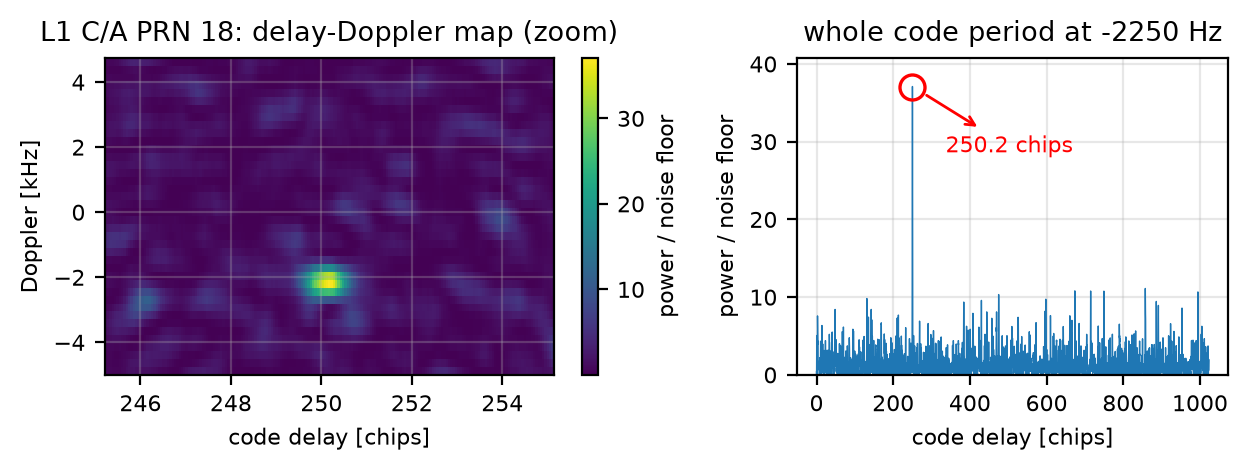
\includegraphics[width=1.0\linewidth]{gnss_sdr/x310_20261022T190000Z/acq_1C.png}
  \caption{Acquisition, L1 C/A: delay--Doppler search of PRN 31; one sharp peak (test statistic 71 vs threshold 47) at 2250~Hz and 248.7~chips.}
\end{figure}

\begin{figure}[H]
  \centering
  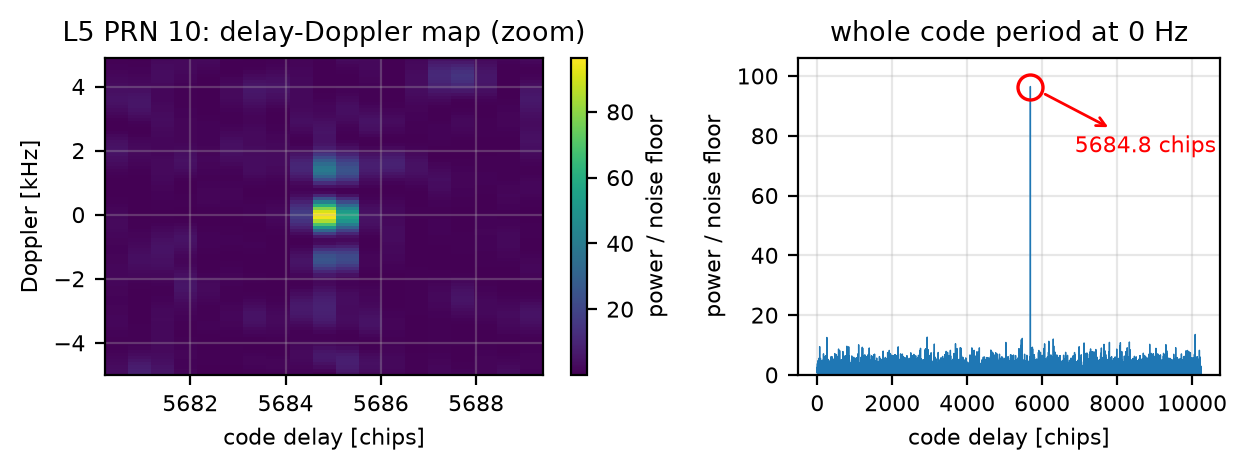
\includegraphics[width=1.0\linewidth]{gnss_sdr/x310_20261022T190000Z/acq_L5.png}
  \caption{Acquisition, L5: delay--Doppler search of PRN 23; one sharp peak (test statistic 51 vs threshold 49) at -1587~Hz and 938.1~chips.}
\end{figure}

\begin{table}[H]
  \centering
  \footnotesize
  \resizebox{\ifdim\width>\linewidth\linewidth\else\width\fi}{!}{%
  \begin{tabular}{lrrrr}
    \hline
    \textbf{Band} & \textbf{Attempts} & \textbf{Detections} & \textbf{Detected PRNs} & \textbf{Best statistic / threshold} \\
    \hline
    L1 C/A & 11 & 1 & 31 & 1.5 \\
    L5 & 115 & 1 & 23 & 1.0 \\
    \hline
  \end{tabular}}
  \caption{Acquisition: search attempts of the dumped channel. Attempts on satellites that are not in view (or, for L5/L2C, do not broadcast that signal) are rejected below the threshold.}
\end{table}

\subsubsection{Tracking}
Code (DLL) and carrier (PLL) loops per satellite.

\begin{figure}[H]
  \centering
  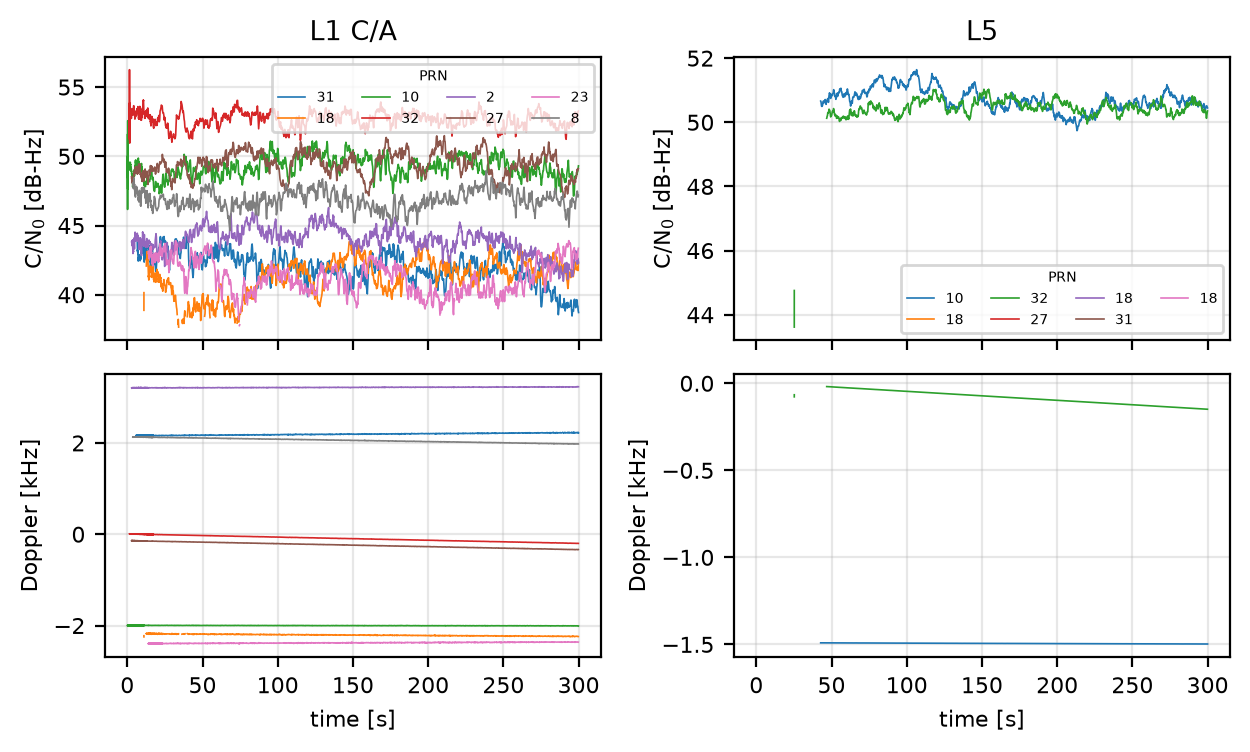
\includegraphics[width=1.0\linewidth]{gnss_sdr/x310_20261022T190000Z/tracking.png}
  \caption{Tracking: carrier-to-noise density ratio and carrier Doppler per satellite, while phase-locked (smooth Doppler curves = loops following the real satellite motion).}
\end{figure}

\begin{figure}[H]
  \centering
  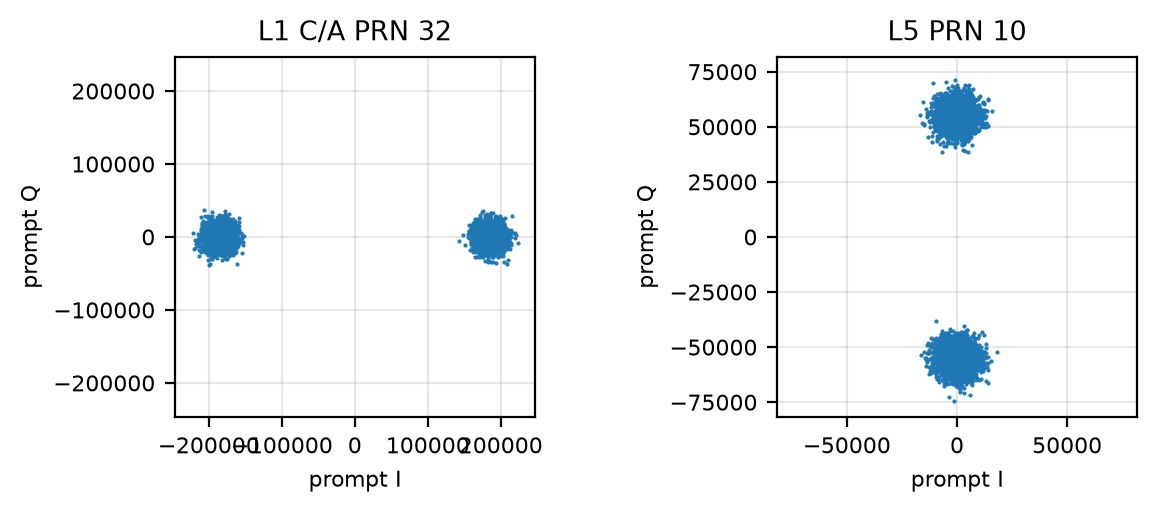
\includegraphics[width=1.0\linewidth]{gnss_sdr/x310_20261022T190000Z/tracking_iq.png}
  \caption{Tracking: prompt correlator outputs of the strongest satellite per band. Two tight clusters on one axis (the $\pm1$ data bits; GNSS-SDR's L5 tracking puts the data component on the Q axis) mean the PLL is phase-locked; a ring would mean it is not.}
\end{figure}

\begin{table}[H]
  \centering
  \footnotesize
  \resizebox{\ifdim\width>\linewidth\linewidth\else\width\fi}{!}{%
  \begin{tabular}{lrrrrrr}
    \hline
    \textbf{Band} & \textbf{Ch.} & \textbf{PRN} & \textbf{Median C/N$_0$ [dB-Hz]} & \textbf{Phase-locked [\%]} & \textbf{Losses of lock} & \textbf{Tracked [s]} \\
    \hline
    L1 C/A & 0 & 31 & 42.7 & 93 & 0 & 561 \\
    L1 C/A & 1 & 2 & 43.5 & 95 & 0 & 28 \\
    L1 C/A & 2 & 10 & 49.2 & 100 & 0 & 512 \\
    L1 C/A & 3 & 32 & 52.9 & 100 & 0 & 30 \\
    L1 C/A & 4 & 28 & 43.8 & 93 & 0 & 526 \\
    L1 C/A & 5 & 27 & 49.0 & 94 & 0 & 528 \\
    L1 C/A & 6 & 8 & 47.0 & 92 & 0 & 30 \\
    L1 C/A & 7 & 23 & 41.9 & 92 & 0 & 530 \\
    L5 & 8 & 23 & 43.5 & 95 & 0 & 372 \\
    L5 & 9 & 8 & 41.7 & 67 & 0 & 374 \\
    L5 & 10 & 28 & 46.4 & 58 & 1 & 279 \\
    L5 & 10 & 32 & 28.9 & 0 & 1 & 16 \\
    L5 & 11 & 32 & 50.4 & 66 & 0 & 327 \\
    L5 & 12 & 2 & 28.8 & 0 & 1 & 16 \\
    L5 & 13 & 10 & 29.2 & 1 & 5 & 32 \\
    L5 & 13 & 31 & 28.7 & 0 & 5 & 48 \\
    L5 & 14 & 27 & 48.2 & 56 & 1 & 279 \\
    L5 & 14 & 32 & 28.9 & 0 & 1 & 16 \\
    L5 & 15 & 10 & 32.2 & 36 & 3 & 51 \\
    L5 & 15 & 27 & 28.8 & 0 & 3 & 16 \\
    \hline
  \end{tabular}}
  \caption{Tracking: per channel and satellite (phase-locked: carrier lock test $> 0.8$).}
\end{table}

\subsubsection{Telemetry decoder}
Navigation-message decoding: bit/frame synchronization, parity/CRC, the ephemeris, and the satellite transmit time (time of week) of every measurement.

\begin{figure}[H]
  \centering
  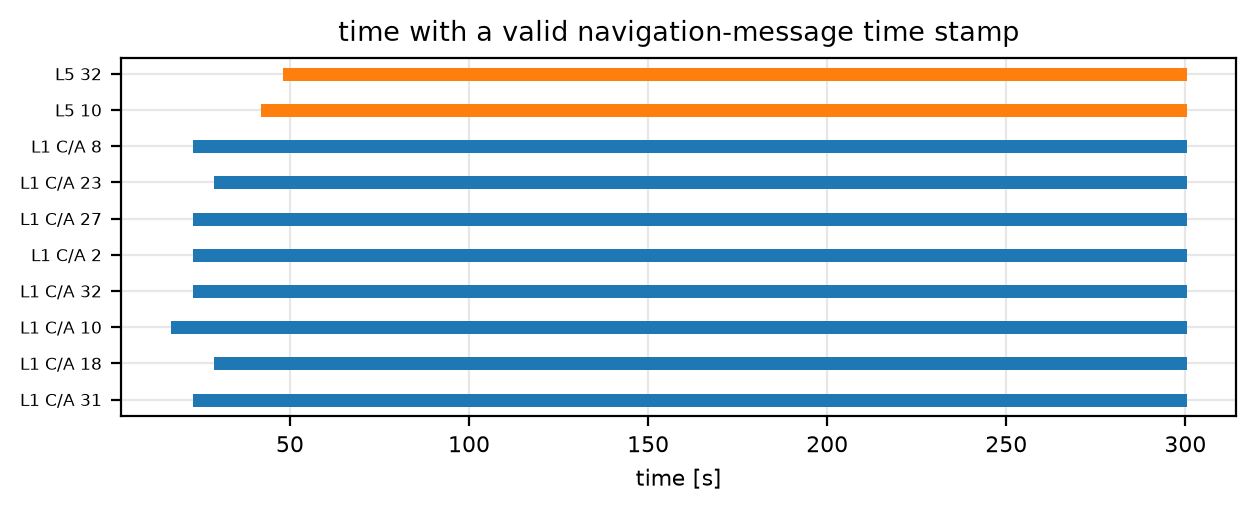
\includegraphics[width=1.0\linewidth]{gnss_sdr/x310_20261022T190000Z/telemetry.png}
  \caption{Telemetry decoder: per band and satellite, when the decoder delivered a valid transmit time (the first one comes after the first complete frame/message).}
\end{figure}

\begin{table}[H]
  \centering
  \footnotesize
  \resizebox{\ifdim\width>\linewidth\linewidth\else\width\fi}{!}{%
  \begin{tabular}{lrrrrr}
    \hline
    \textbf{Band} & \textbf{PRN} & \textbf{Messages decoded} & \textbf{Ephemeris} & \textbf{First valid at [s]} & \textbf{TOW [s]} \\
    \hline
    L1 C/A & 2 & 44 & yes & 41.1 & 414066.0 \\
    L1 C/A & 8 & 46 & yes & 23.1 & 414048.0 \\
    L1 C/A & 10 & 48 & yes & 17.1 & 414042.0 \\
    L1 C/A & 23 & 46 & yes & 23.1 & 414048.0 \\
    L1 C/A & 27 & 47 & yes & 23.1 & 414048.0 \\
    L1 C/A & 28 & 44 & yes & 29.1 & 414054.0 \\
    L1 C/A & 31 & 47 & yes & 23.1 & 414048.0 \\
    L1 C/A & 32 & 47 & yes & 23.1 & 414048.0 \\
    L5 & 8 & 25 & yes & 48.1 & 414073.0 \\
    L5 & 10 & 7 & yes & 228.4 & 414253.3 \\
    L5 & 23 & 31 & yes & 48.1 & 414073.0 \\
    L5 & 27 & 15 & yes & 144.1 & 414169.0 \\
    L5 & 28 & 19 & yes & 144.1 & 414169.0 \\
    L5 & 32 & 22 & yes & 90.0 & 414114.9 \\
    \hline
  \end{tabular}}
  \caption{Telemetry decoder: L1 C/A LNAV subframes and L2C/L5 CNAV messages decoded, ephemeris obtained, and the first valid time of week.}
\end{table}

\subsubsection{Observables}
Pseudorange, carrier phase and Doppler of every channel at common receiver epochs.

\begin{figure}[H]
  \centering
  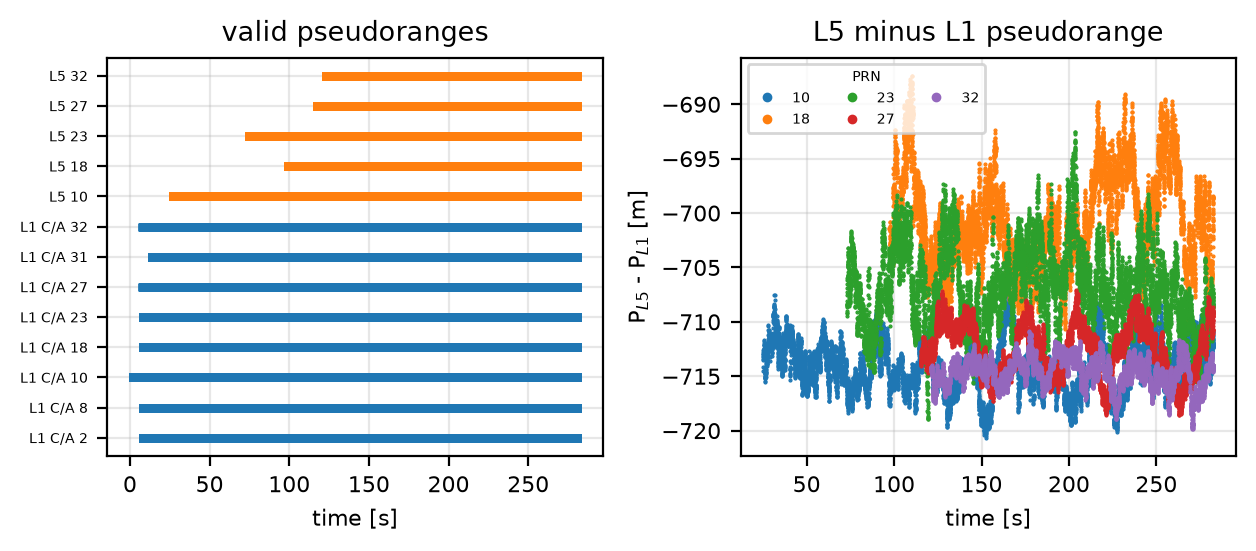
\includegraphics[width=1.0\linewidth]{gnss_sdr/x310_20261022T190000Z/observables.png}
  \caption{Observables: epochs with a valid pseudorange per band and satellite, and the difference between the two bands' pseudoranges of the same satellite (a constant receiver inter-band bias, the same for every satellite, plus the slowly varying ionospheric delay).}
\end{figure}

\begin{table}[H]
  \centering
  \footnotesize
  \resizebox{\ifdim\width>\linewidth\linewidth\else\width\fi}{!}{%
  \begin{tabular}{lrrrrr}
    \hline
    \textbf{PRN} & \textbf{Common epochs} & \textbf{of run [\%]} & \textbf{Mean [m]} & \textbf{Std [m]} & \textbf{Drift [m/s]} \\
    \hline
    8 & 12228 & 82 & -710.75 & 2.19 & 0.0014 \\
    10 & 3563 & 24 & -713.39 & 2.20 & 0.0208 \\
    23 & 12231 & 82 & -707.12 & 3.91 & 0.0006 \\
    27 & 7627 & 51 & -712.62 & 2.45 & -0.0107 \\
    28 & 7628 & 51 & -702.35 & 2.80 & 0.0221 \\
    32 & 10330 & 69 & -714.67 & 1.54 & -0.0003 \\
    \hline
  \end{tabular}}
  \caption{Observables: P$_{\mathrm{L5}}$ $-$ P$_{\mathrm{L1}}$ per satellite at common epochs (similar means = shared receiver bias; std = code noise of both bands).}
\end{table}

\subsubsection{PVT}
Position from the pseudoranges and the decoded ephemeris, compared with the surveyed antenna position (-23.209433$^\circ$, -45.874875$^\circ$, 596.42~m).

\begin{figure}[H]
  \centering
  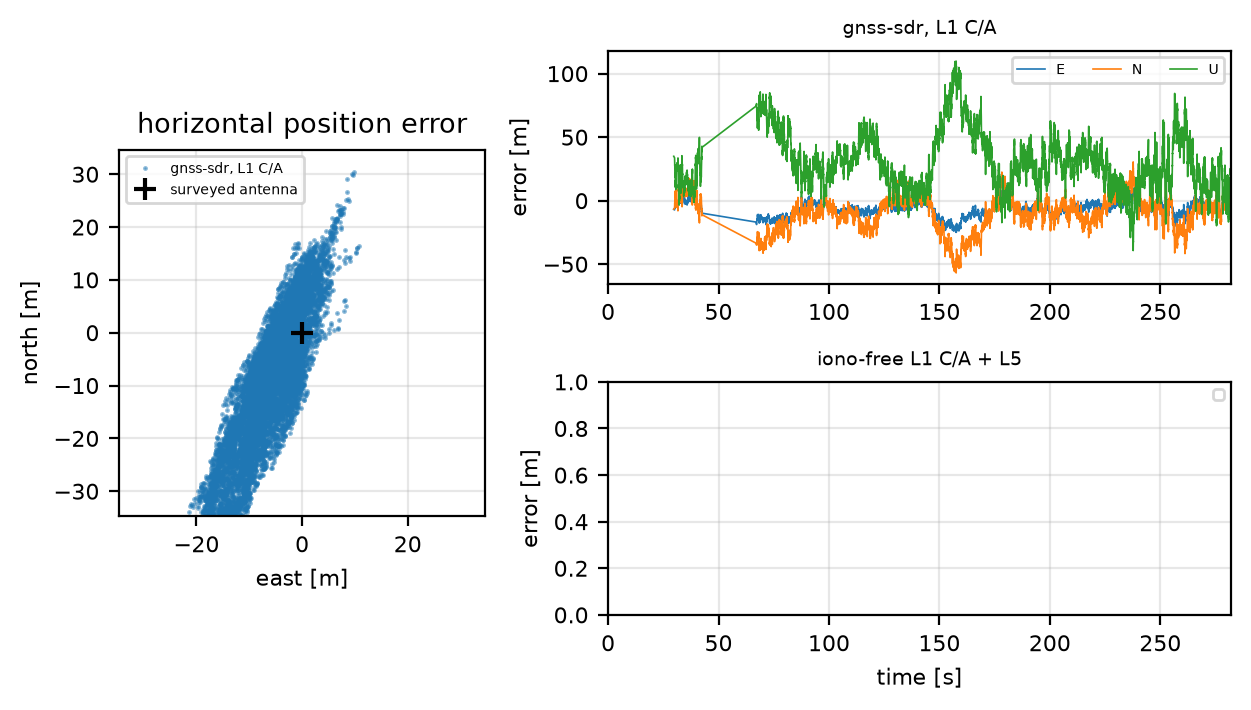
\includegraphics[width=1.0\linewidth]{gnss_sdr/x310_20261022T190000Z/pvt.png}
  \caption{PVT: position error with respect to the surveyed antenna position. L1 C/A: gnss-sdr's own solution (broadcast ionosphere model). Iono-free: computed from gnss-sdr's observables and decoded ephemeris (gnss\_spp.py), removing the ionospheric delay with the second band (pseudoranges carrier-smoothed over 100~s).}
\end{figure}

\begin{figure}[H]
  \centering
  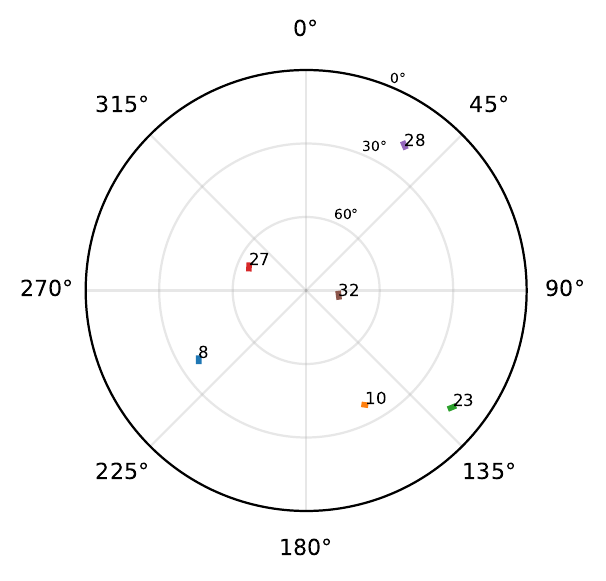
\includegraphics[width=0.45\linewidth]{gnss_sdr/x310_20261022T190000Z/skyplot.png}
  \caption{PVT: sky plot of the satellites in the dual-frequency solution (azimuth, elevation) during the recording.}
\end{figure}

\begin{table}[H]
  \centering
  \footnotesize
  \resizebox{\ifdim\width>\linewidth\linewidth\else\width\fi}{!}{%
  \begin{tabular}{lcc}
    \hline
    \textbf{Solution} & \textbf{gnss-sdr, L1 C/A} & \textbf{iono-free L1 C/A + L5} \\
    \hline
    Solutions & 10332 & 151 \\
    Run with fix [\%] & 72 & 54 \\
    Mean E / N / U [m] & -2.0 / -1.5 / 20.0 & -7.0 / 8.2 / -2.9 \\
    Std E / N / U [m] & 3.2 / 4.5 / 3.6 & 5.0 / 6.7 / 7.9 \\
    RMS 2-D [m] & 6.1 & 13.6 \\
    RMS 3-D [m] & 21.2 & 16.0 \\
    95\% horiz. [m] & 9.3 & 20.6 \\
    \hline
  \end{tabular}}
  \caption{PVT: position error statistics with respect to the surveyed antenna (mean = accuracy, std = precision; \% of the run's seconds with a position; gnss-sdr outputs several solutions per second, the iono-free one is computed once per second).}
\end{table}


\subsubsection{Signal conditioner (Galileo E1 + E5a)}


\begin{table}[H]
  \centering
  \footnotesize
  \resizebox{\ifdim\width>\linewidth\linewidth\else\width\fi}{!}{%
  \begin{tabular}{l>{\centering\arraybackslash}p{4.2cm}>{\centering\arraybackslash}p{4.2cm}}
    \hline
    \textbf{Channel} & \textbf{ch0 (Galileo E1)} & \textbf{ch1 (Galileo E5a)} \\
    \hline
    File format & ci8 & ci8 \\
    Source item type & ibyte & ibyte \\
    Data type adapter & Ibyte\_To\_Complex & Ibyte\_To\_Complex \\
    Input filter & Pass\_Through & Pass\_Through \\
    Resampling & $\times$5 zero-order hold, offline (\texttt{upsample\_iq.py}) & Pass\_Through \\
    Rate [MS/s] & 4 $\to$ 20 & 20 $\to$ 20 \\
    \hline
  \end{tabular}}
  \caption{Signal conditioner: recorded format and rate to gnss-sdr's internal \texttt{gr\_complex} stream; both bands are read in lockstep by one \texttt{Multichannel\_File\_Signal\_Source}.}
\end{table}

\subsubsection{Acquisition (Galileo E1 + E5a)}
Two-dimensional search over code delay and Doppler (one channel per band dumped; the others behave alike).

\begin{figure}[H]
  \centering
  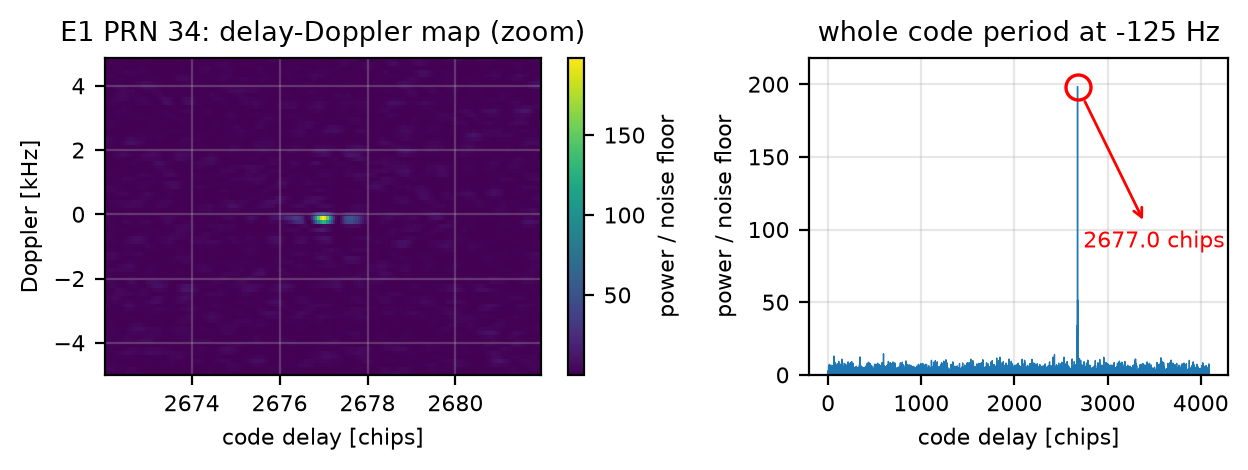
\includegraphics[width=1.0\linewidth]{gnss_sdr/x310_20261022T190000Z/galileo_acq_1B.png}
  \caption{Acquisition, Galileo E1: delay--Doppler search of PRN 34; one sharp peak (test statistic 272 vs threshold 52) at -125~Hz and 2677.0~chips.}
\end{figure}

\begin{figure}[H]
  \centering
  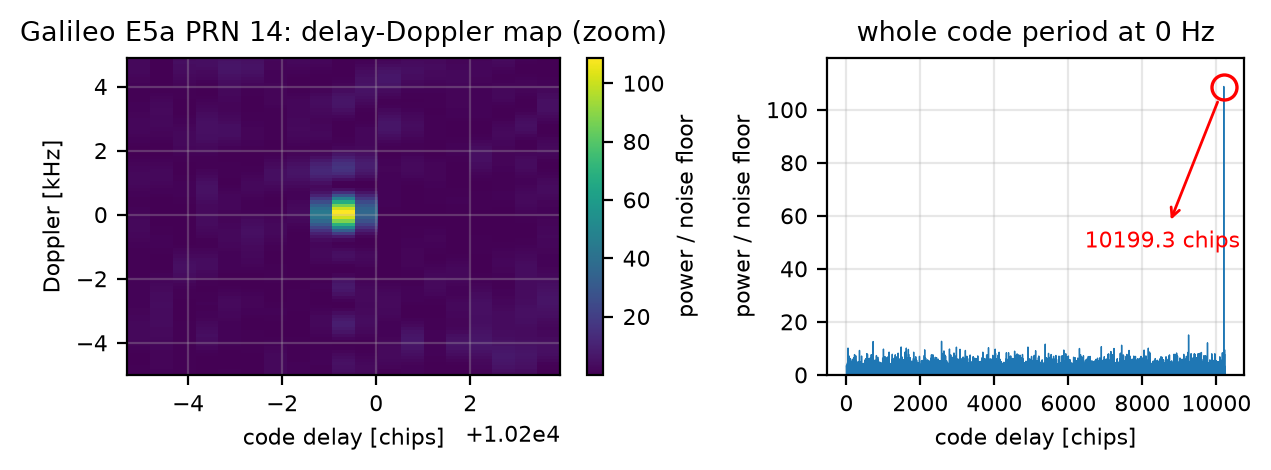
\includegraphics[width=1.0\linewidth]{gnss_sdr/x310_20261022T190000Z/galileo_acq_5X.png}
  \caption{Acquisition, Galileo E5a: delay--Doppler search of PRN 14; one sharp peak (test statistic 149 vs threshold 49) at -1427~Hz and 10199.3~chips.}
\end{figure}

\begin{table}[H]
  \centering
  \footnotesize
  \resizebox{\ifdim\width>\linewidth\linewidth\else\width\fi}{!}{%
  \begin{tabular}{lrrrr}
    \hline
    \textbf{Band} & \textbf{Attempts} & \textbf{Detections} & \textbf{Detected PRNs} & \textbf{Best statistic / threshold} \\
    \hline
    Galileo E1 & 5 & 1 & 34 & 5.3 \\
    Galileo E5a & 2 & 2 & 14 & 3.0 \\
    \hline
  \end{tabular}}
  \caption{Acquisition: search attempts of the dumped channel. Attempts on satellites that are not in view (or do not broadcast that signal, e.g. older GPS satellites on L5/L2C) are rejected below the threshold.}
\end{table}

\subsubsection{Tracking (Galileo E1 + E5a)}


\begin{figure}[H]
  \centering
  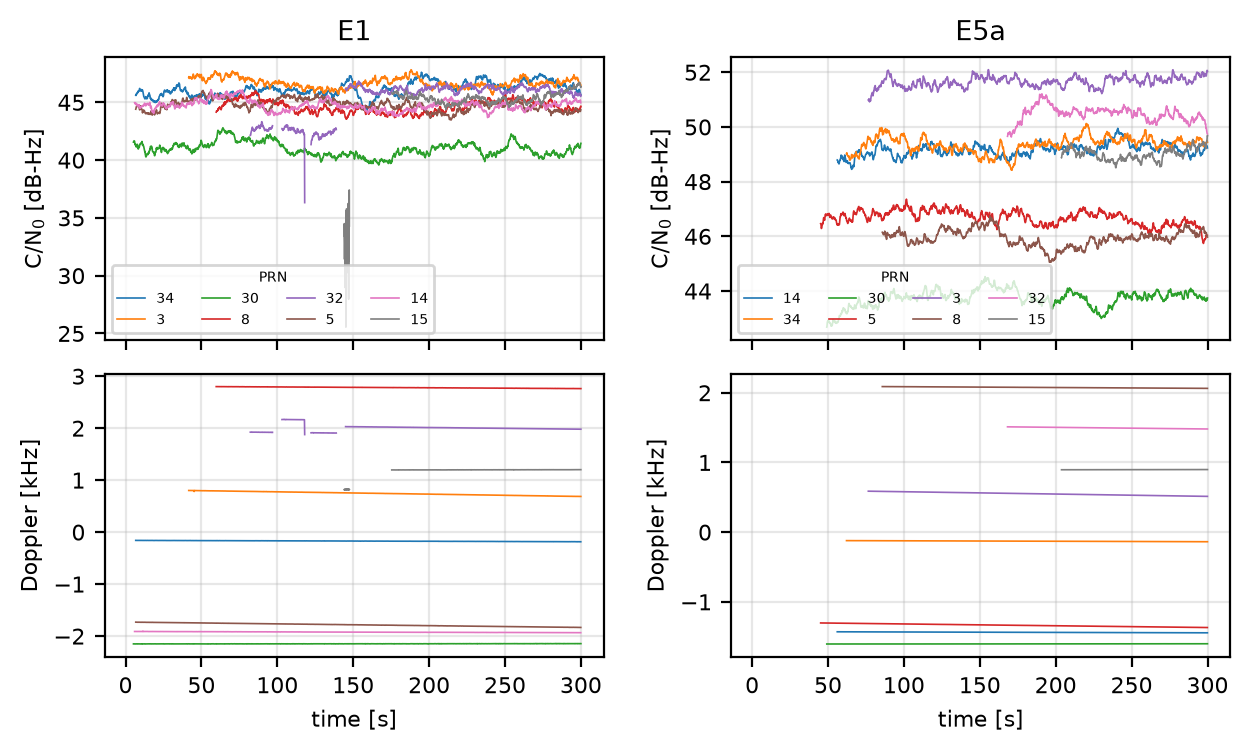
\includegraphics[width=1.0\linewidth]{gnss_sdr/x310_20261022T190000Z/galileo_tracking.png}
  \caption{Tracking: carrier-to-noise density ratio and carrier Doppler per satellite, while phase-locked (smooth Doppler curves = loops following the real satellite motion).}
\end{figure}

\begin{figure}[H]
  \centering
  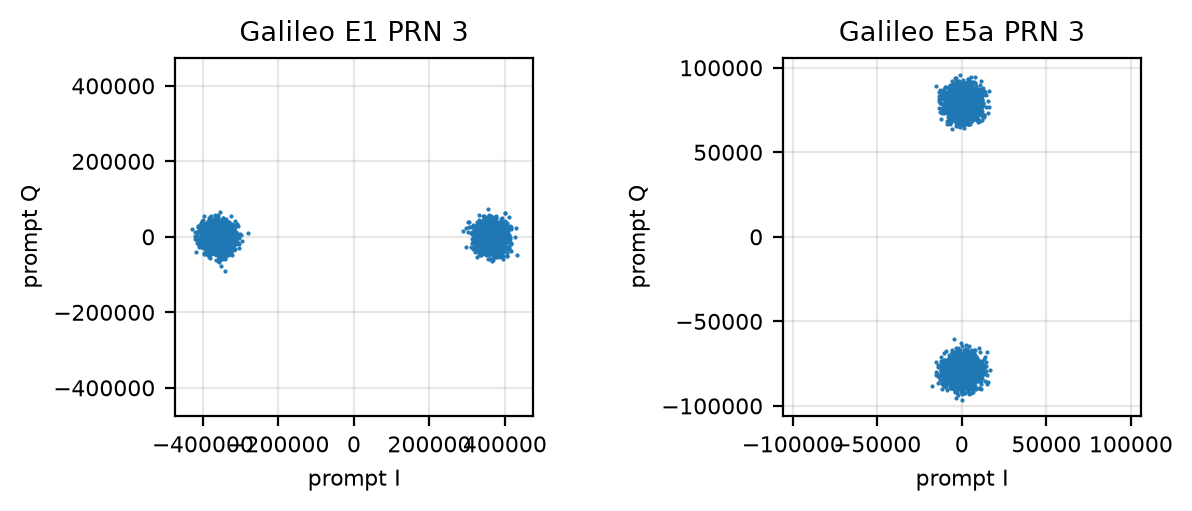
\includegraphics[width=1.0\linewidth]{gnss_sdr/x310_20261022T190000Z/galileo_tracking_iq.png}
  \caption{Tracking: prompt correlator outputs of the strongest satellite per band. Two tight clusters on one axis (the $\pm1$ data bits; GNSS-SDR's L5 tracking puts the data component on the Q axis), or a single one for a dataless pilot (Galileo E1-C and E5a-Q, tracked here), mean the PLL is phase-locked; a ring would mean it is not. \texttt{Prompt\_I}/\texttt{Prompt\_Q} are 32-bit floats (sums of the samples over one integration period, in file units): they never clip, only overflowing beyond $\pm 3.4\times10^{38}$, far above the $N\cdot\text{full scale}\cdot\sqrt{2}$ a sum of $N$ samples can reach.}
\end{figure}

\begin{table}[H]
  \centering
  \footnotesize
  \resizebox{\ifdim\width>\linewidth\linewidth\else\width\fi}{!}{%
  \begin{tabular}{lrrrrrr}
    \hline
    \textbf{Band} & \textbf{Ch.} & \textbf{PRN} & \textbf{Median C/N$_0$ [dB-Hz]} & \textbf{Phase-locked [\%]} & \textbf{Losses of lock} & \textbf{Tracked [s]} \\
    \hline
    Galileo E1 & 0 & 34 & 46.1 & 98 & 0 & 299 \\
    Galileo E1 & 1 & 3 & 46.6 & 87 & 2 & 298 \\
    Galileo E1 & 2 & 30 & 40.9 & 99 & 0 & 299 \\
    Galileo E1 & 3 & 8 & 44.4 & 81 & 2 & 298 \\
    Galileo E1 & 4 & 32 & 45.7 & 68 & 7 & 299 \\
    Galileo E1 & 5 & 5 & 44.8 & 98 & 0 & 298 \\
    Galileo E1 & 6 & 14 & 44.7 & 98 & 0 & 300 \\
    Galileo E1 & 7 & 15 & 44.5 & 43 & 8 & 300 \\
    Galileo E5a & 8 & 14 & 48.9 & 31 & 1 & 275 \\
    Galileo E5a & 9 & 34 & 48.9 & 30 & 1 & 274 \\
    Galileo E5a & 10 & 30 & 43.5 & 52 & 0 & 272 \\
    Galileo E5a & 11 & 5 & 46.8 & 53 & 0 & 274 \\
    Galileo E5a & 12 & 3 & 51.6 & 49 & 0 & 244 \\
    Galileo E5a & 13 & 8 & 45.9 & 48 & 0 & 235 \\
    Galileo E5a & 14 & 32 & 50.4 & 37 & 0 & 144 \\
    Galileo E5a & 15 & 15 & 49.0 & 30 & 0 & 114 \\
    \hline
  \end{tabular}}
  \caption{Tracking: per channel and satellite (phase-locked: carrier lock test $> 0.8$).}
\end{table}

\subsubsection{Telemetry decoder (Galileo E1 + E5a)}


\begin{figure}[H]
  \centering
  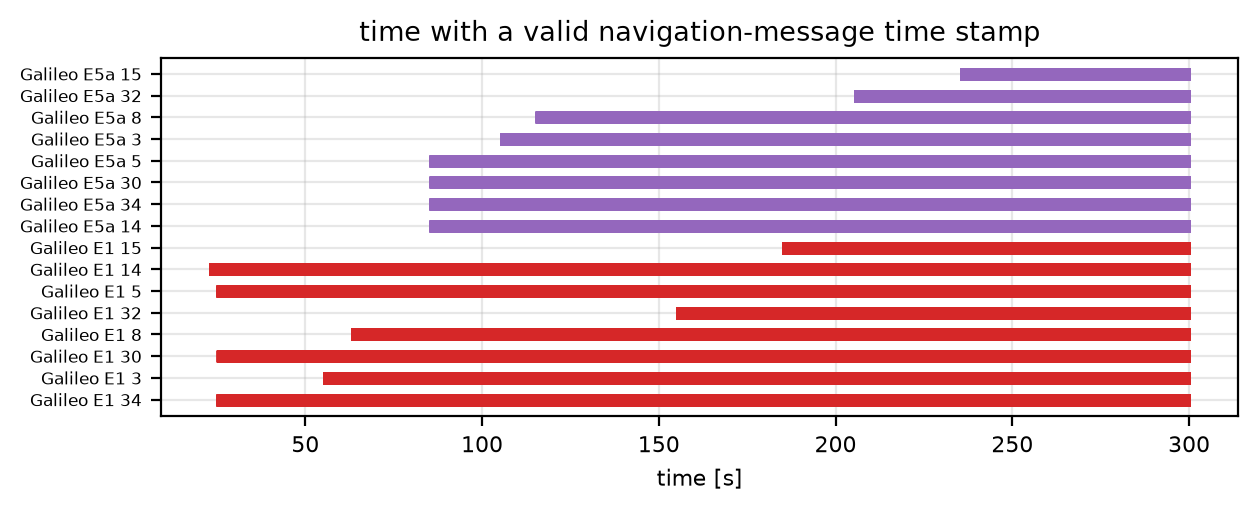
\includegraphics[width=1.0\linewidth]{gnss_sdr/x310_20261022T190000Z/galileo_telemetry.png}
  \caption{Telemetry decoder: per band and satellite, when the decoder delivered a valid transmit time (the first one comes after the first complete frame/message).}
\end{figure}

\begin{table}[H]
  \centering
  \footnotesize
  \resizebox{\ifdim\width>\linewidth\linewidth\else\width\fi}{!}{%
  \begin{tabular}{lrrrrr}
    \hline
    \textbf{Band} & \textbf{PRN} & \textbf{Messages decoded} & \textbf{Ephemeris} & \textbf{First valid at [s]} & \textbf{TOW [s]} \\
    \hline
    Galileo E1 & 3 & 24 & yes & 55.2 & 414080.0 \\
    Galileo E1 & 5 & 26 & yes & 25.2 & 414050.0 \\
    Galileo E1 & 8 & 23 & yes & 63.2 & 414088.0 \\
    Galileo E1 & 14 & 26 & yes & 23.2 & 414048.0 \\
    Galileo E1 & 15 & 10 & yes & 185.2 & 414210.0 \\
    Galileo E1 & 30 & 26 & yes & 25.2 & 414050.0 \\
    Galileo E1 & 32 & 13 & yes & 155.2 & 414180.0 \\
    Galileo E1 & 34 & 26 & yes & 25.2 & 414050.0 \\
    Galileo E5a & 3 & 11 & yes & 105.4 & 414130.3 \\
    Galileo E5a & 5 & 12 & yes & 85.4 & 414110.3 \\
    Galileo E5a & 8 & 10 & yes & 115.4 & 414140.3 \\
    Galileo E5a & 14 & 11 & yes & 85.4 & 414110.3 \\
    Galileo E5a & 15 & 3 & yes & 235.4 & 414260.3 \\
    Galileo E5a & 30 & 12 & yes & 85.4 & 414110.3 \\
    Galileo E5a & 32 & 5 & yes & 205.4 & 414230.3 \\
    Galileo E5a & 34 & 12 & yes & 85.4 & 414110.3 \\
    \hline
  \end{tabular}}
  \caption{Telemetry decoder: Galileo E1 I/NAV words, Galileo E5a F/NAV pages decoded, ephemeris obtained, and the first valid time of week.}
\end{table}

\subsubsection{Observables (Galileo E1 + E5a)}
Pseudorange, carrier phase and Doppler of every channel at common receiver epochs.

\begin{figure}[H]
  \centering
  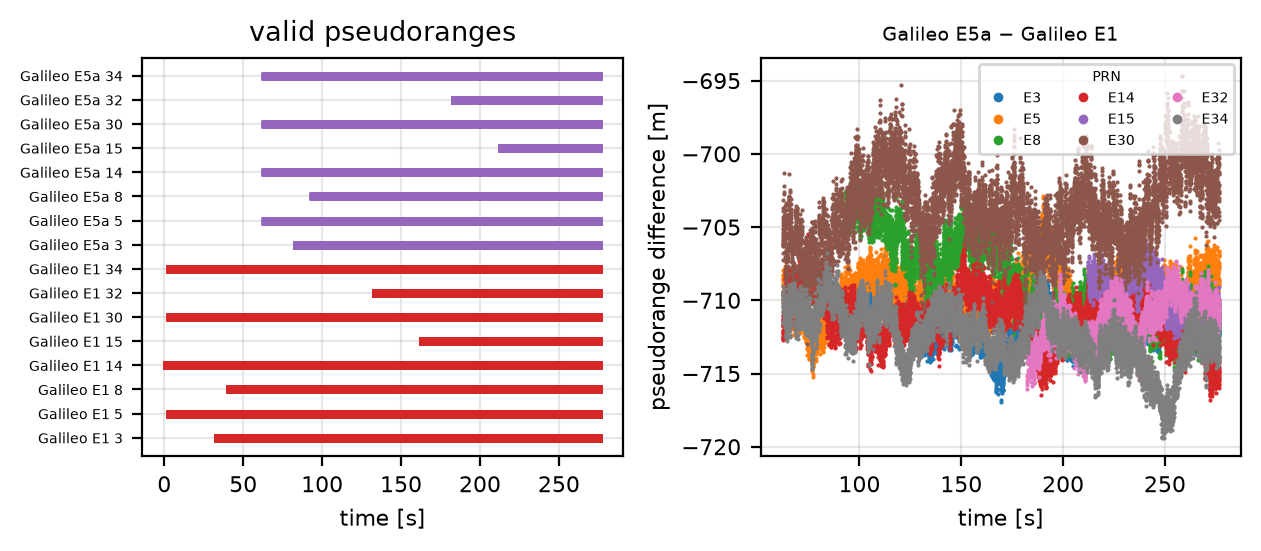
\includegraphics[width=1.0\linewidth]{gnss_sdr/x310_20261022T190000Z/galileo_observables.png}
  \caption{Observables: epochs with a valid pseudorange per band and satellite, and the difference between the two bands' pseudoranges of the same satellite (a constant receiver inter-band bias, the same for every satellite, plus the slowly varying ionospheric delay).}
\end{figure}

\begin{table}[H]
  \centering
  \footnotesize
  \resizebox{\ifdim\width>\linewidth\linewidth\else\width\fi}{!}{%
  \begin{tabular}{lrrrrrr}
    \hline
    \textbf{Difference} & \textbf{PRN} & \textbf{Common epochs} & \textbf{of run [\%]} & \textbf{Mean [m]} & \textbf{Std [m]} & \textbf{Drift [m/s]} \\
    \hline
    Galileo E5a $-$ Galileo E1 & 3 & 9563 & 64 & -711.43 & 1.45 & -0.0075 \\
    Galileo E5a $-$ Galileo E1 & 5 & 10437 & 70 & -709.61 & 1.55 & 0.0065 \\
    Galileo E5a $-$ Galileo E1 & 8 & 9128 & 61 & -708.81 & 2.89 & -0.0451 \\
    Galileo E5a $-$ Galileo E1 & 14 & 10437 & 70 & -711.16 & 1.64 & -0.0082 \\
    Galileo E5a $-$ Galileo E1 & 15 & 3147 & 21 & -709.62 & 1.46 & -0.0504 \\
    Galileo E5a $-$ Galileo E1 & 30 & 10457 & 70 & -703.72 & 2.59 & 0.0079 \\
    Galileo E5a $-$ Galileo E1 & 32 & 4647 & 31 & -711.39 & 1.51 & 0.0347 \\
    Galileo E5a $-$ Galileo E1 & 34 & 10437 & 70 & -712.45 & 1.88 & -0.0177 \\
    \hline
  \end{tabular}}
  \caption{Observables: pseudorange difference between the two bands of each satellite at common epochs (similar means = shared receiver bias; std = code noise of both bands).}
\end{table}

\subsubsection{PVT (Galileo E1 + E5a)}
Position from the pseudoranges and the decoded ephemeris, compared with the surveyed antenna position (-23.209433$^\circ$, -45.874875$^\circ$, 596.42~m).

\begin{figure}[H]
  \centering
  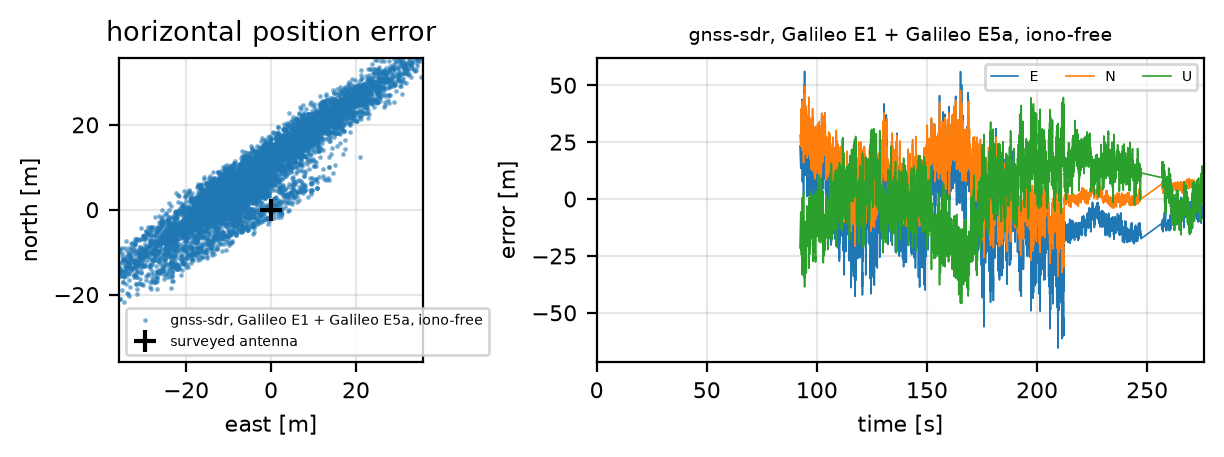
\includegraphics[width=1.0\linewidth]{gnss_sdr/x310_20261022T190000Z/galileo_pvt.png}
  \caption{PVT: position error with respect to the surveyed antenna position. gnss-sdr: GNSS-SDR's own RTKLIB solution.}
\end{figure}

\begin{table}[H]
  \centering
  \footnotesize
  \resizebox{\ifdim\width>\linewidth\linewidth\else\width\fi}{!}{%
  \begin{tabular}{l>{\centering\arraybackslash}p{4.2cm}}
    \hline
    \textbf{Solution} & \textbf{gnss-sdr, Galileo E1 + Galileo E5a, iono-free} \\
    \hline
    Solutions & 8642 \\
    Run with fix [\%] & 64 \\
    Mean E / N / U [m] & -4.8 / 6.7 / 2.8 \\
    Std E / N / U [m] & 15.5 / 11.9 / 14.2 \\
    RMS 2-D [m] & 21.2 \\
    RMS 3-D [m] & 25.6 \\
    95\% horiz. [m] & 40.3 \\
    \hline
  \end{tabular}}
  \caption{PVT: position error statistics with respect to the surveyed antenna (mean = accuracy, std = precision; \% of the run's seconds with a position; gnss-sdr outputs several solutions per second, gnss\_spp.py computes one per second).}
\end{table}




\subsection{Second record}
\begin{table}[H]
  \centering
  \begin{tabular}{|l|l|l|}
    \hline
    \textbf{Parameter} & \textbf{Channel 0} & \textbf{Channel 1} \\
    \hline
    Start time & \multicolumn{2}{>{\centering\arraybackslash}p{7cm}|}{2026-10-22 19:30:07 UTC} \\
    \hline
    Frequency & 1575.420 MHz (L1) & 1227.600 MHz (L2) \\
    \hline
    Duration & 300.0 s & 300.0 s \\
    \hline
    Sample rate & 4.000 MS/s & 4.000 MS/s \\
    \hline
    Sample type & \multicolumn{2}{>{\centering\arraybackslash}p{7cm}|}{signed complex 16-bit samples (I+Q), little-endian, as received from the X310 (sc16)} \\
    \hline
    Gain & 25.0 dB & 25.0 dB \\
    \hline
    Antenna & RX1 & RX2 \\
    \hline
    File size & 4800.0 MB & 4800.0 MB \\
    \hline
    Samples written & 1,200,000,000 & 1,200,000,000 \\
    \hline
    Lost samples & 0 & 0 \\
    \hline
    Clock source & \multicolumn{2}{>{\centering\arraybackslash}p{7cm}|}{external} \\
    \hline
    Time source & \multicolumn{2}{>{\centering\arraybackslash}p{7cm}|}{internal} \\
    \hline
    Motherboard & \multicolumn{2}{>{\centering\arraybackslash}p{7cm}|}{USRP X310} \\
    \hline
    Daughterboard & TwinRX RX0 & TwinRX RX1 \\
    \hline
    Recorder & \multicolumn{2}{>{\centering\arraybackslash}p{7cm}|}{UHD Python API} \\
    \hline
    GNSS-SDR configuration & \multicolumn{2}{>{\centering\arraybackslash}p{7cm}|}{\texttt{l1ca16bits4msps\_l2c16bits4msps.conf}} \\
    \hline
  \end{tabular}
  \caption{Metadata for recording \texttt{x310\_20261022T193000Z}, captured starting 2026-10-22T19:30:07.040026Z.}
\end{table}

\subsubsection{Signal source}
Raw I/Q samples of each channel analysed within the window [10, 10.5]~s after the start recording instant.

\begin{figure}[H]
  \centering
  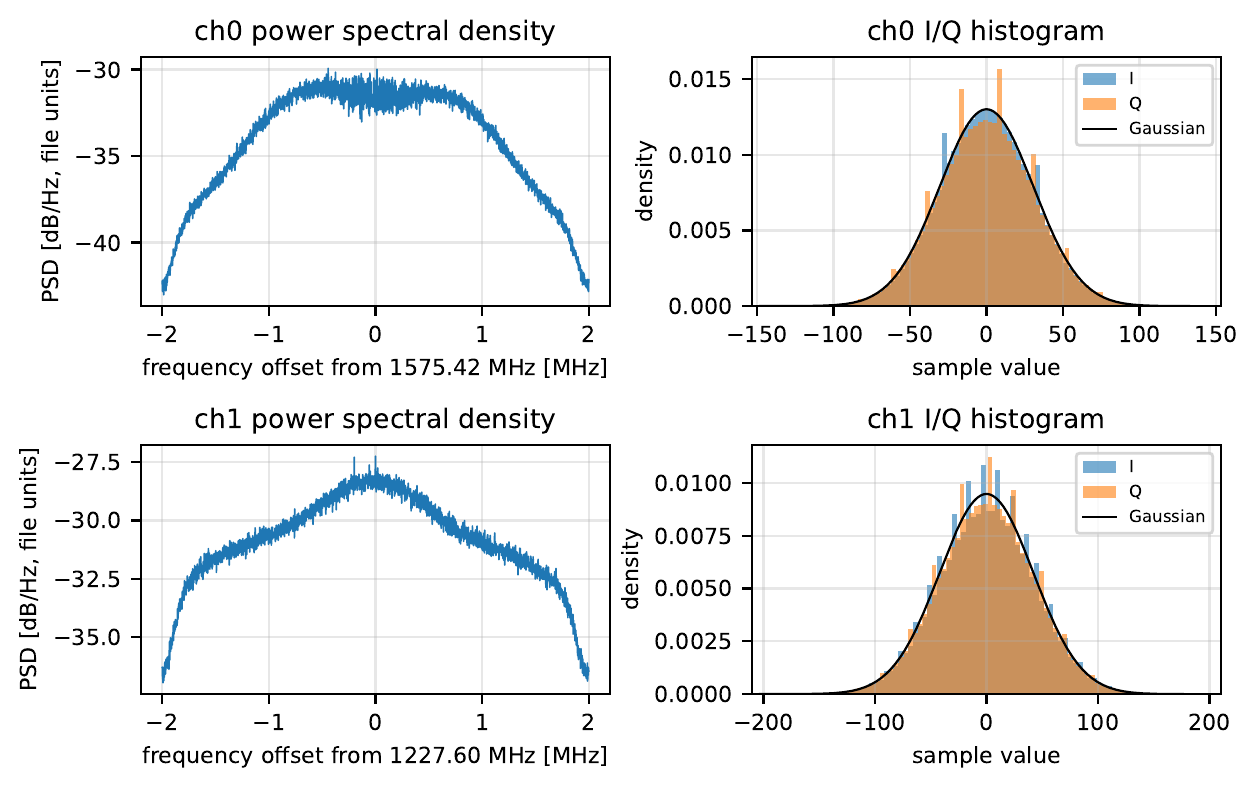
\includegraphics[width=1.0\linewidth]{gnss_sdr/x310_20261022T193000Z/source.png}
  \caption{Signal source: power spectral density (the receiver passband over a flat thermal-noise floor; GNSS signals are below the noise, so only interference would stand out) and I/Q histograms (Gaussian noise, centred, not clipped).}
\end{figure}

\begin{table}[H]
  \centering
  \footnotesize
  \resizebox{\ifdim\width>\linewidth\linewidth\else\width\fi}{!}{%
  \begin{tabular}{l>{\centering\arraybackslash}p{3.8cm}>{\centering\arraybackslash}p{3.8cm}}
    \hline
    \textbf{Channel} & \textbf{ch0} & \textbf{ch1} \\
    \hline
    Frequency [MHz] & 1575.42 & 1227.60 \\
    Rate [MS/s] & 4 & 4 \\
    Format & ci16\_le & ci16\_le \\
    Bytes per complex sample & 4 (2 for I, 2 for Q) & 4 (2 for I, 2 for Q) \\
    Full scale & $\pm$32767 & $\pm$32767 \\
    Gain [dB] & 25 & 25 \\
    Std I / Q & 30.2 / 31.1 & 42.1 / 42.1 \\
    Mean I / Q & -0.04 / -0.13 & 0.28 / 0.05 \\
    Min / max I & -151 / 154 & -227 / 208 \\
    Min / max Q & -150 / 164 & -208 / 210 \\
    Headroom (full scale / std) & 1069.3 & 778.5 \\
    Clipped [\%] & 0.000 & 0.000 \\
    Lost samples & 0 & 0 \\
    \hline
  \end{tabular}}
  \caption{Signal source: sample statistics per channel (headroom: how many standard deviations of the noise fit before clipping).}
\end{table}

\subsubsection{Signal conditioner}


\begin{table}[H]
  \centering
  \footnotesize
  \resizebox{\ifdim\width>\linewidth\linewidth\else\width\fi}{!}{%
  \begin{tabular}{l>{\centering\arraybackslash}p{3.8cm}>{\centering\arraybackslash}p{3.8cm}}
    \hline
    \textbf{Channel} & \textbf{ch0 (L1 C/A)} & \textbf{ch1 (L2C)} \\
    \hline
    File format & ci16\_le & ci16\_le \\
    Source item type & ishort & ishort \\
    Data type adapter & Ishort\_To\_Complex & Ishort\_To\_Complex \\
    Input filter & Pass\_Through & Pass\_Through \\
    Resampling & Pass\_Through & Pass\_Through \\
    Rate [MS/s] & 4 $\to$ 4 & 4 $\to$ 4 \\
    \hline
  \end{tabular}}
  \caption{Signal conditioner: recorded format and rate to gnss-sdr's internal \texttt{gr\_complex} stream; both bands are read in lockstep by one \texttt{Multichannel\_File\_Signal\_Source}.}
\end{table}

\subsubsection{Acquisition}
Two-dimensional search over code delay and Doppler (one channel per band dumped; the others behave alike).

\begin{figure}[H]
  \centering
  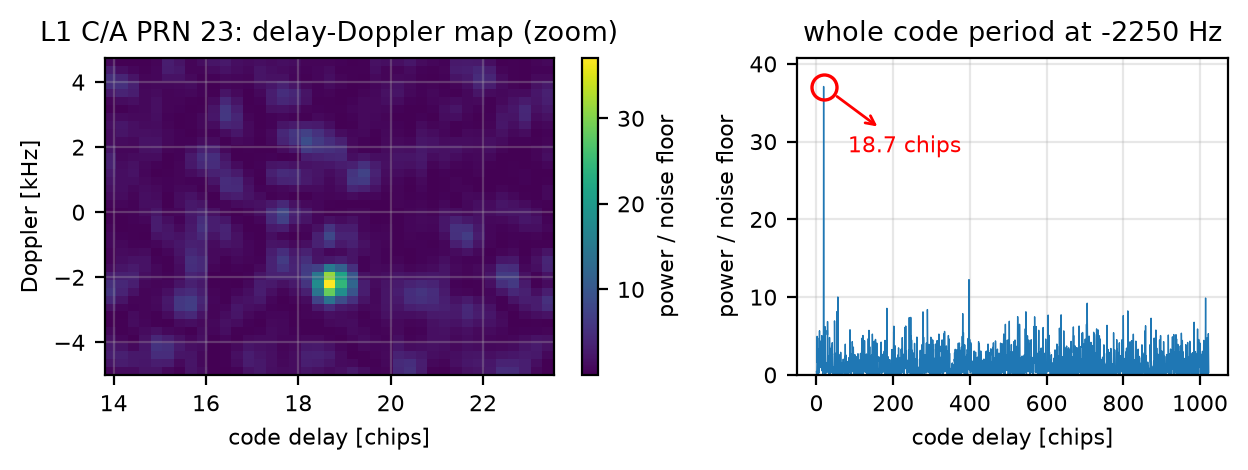
\includegraphics[width=1.0\linewidth]{gnss_sdr/x310_20261022T193000Z/acq_1C.png}
  \caption{Acquisition, L1 C/A: delay--Doppler search of PRN 23; one sharp peak (test statistic 50 vs threshold 44) at -2250~Hz and 18.7~chips.}
\end{figure}

\begin{table}[H]
  \centering
  \footnotesize
  \resizebox{\ifdim\width>\linewidth\linewidth\else\width\fi}{!}{%
  \begin{tabular}{lrrrr}
    \hline
    \textbf{Band} & \textbf{Attempts} & \textbf{Detections} & \textbf{Detected PRNs} & \textbf{Best statistic / threshold} \\
    \hline
    L1 C/A & 3 & 1 & 23 & 1.1 \\
    L2C & \multicolumn{4}{l}{not dumped (search grid too large); acquired satellites: see the tracking table} \\
    \hline
  \end{tabular}}
  \caption{Acquisition: search attempts of the dumped channel. Attempts on satellites that are not in view (or, for L5/L2C, do not broadcast that signal) are rejected below the threshold.}
\end{table}

\subsubsection{Tracking}


\begin{figure}[H]
  \centering
  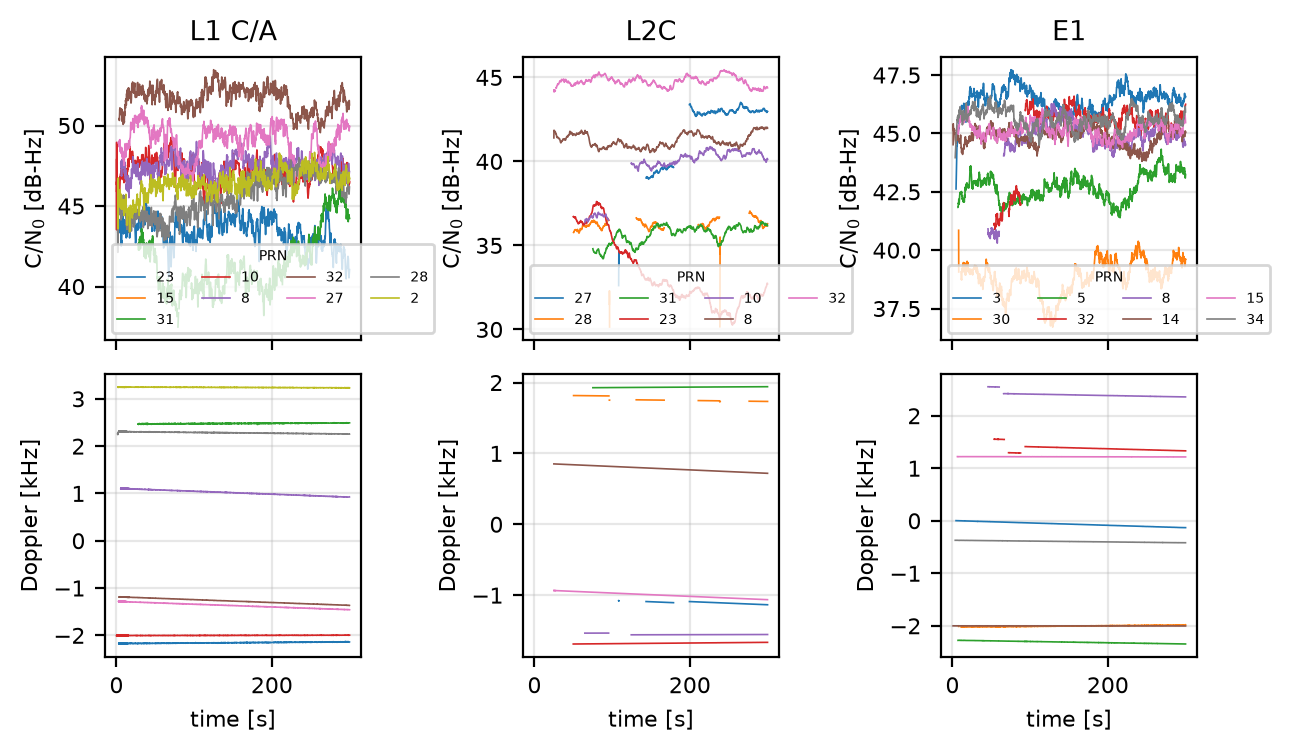
\includegraphics[width=1.0\linewidth]{gnss_sdr/x310_20261022T193000Z/tracking.png}
  \caption{Tracking: carrier-to-noise density ratio and carrier Doppler per satellite, while phase-locked (smooth Doppler curves = loops following the real satellite motion).}
\end{figure}

\begin{figure}[H]
  \centering
  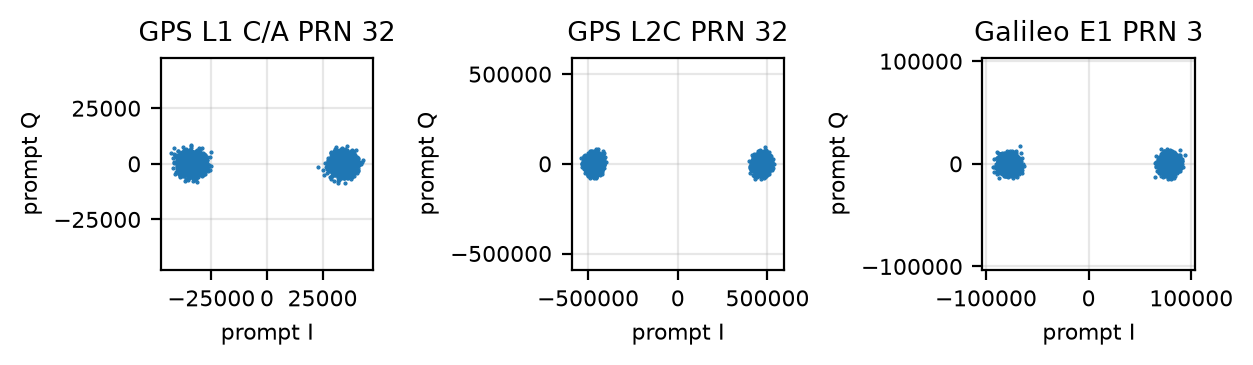
\includegraphics[width=1.0\linewidth]{gnss_sdr/x310_20261022T193000Z/tracking_iq.png}
  \caption{Tracking: prompt correlator outputs of the strongest satellite per band. Two tight clusters on one axis (the $\pm1$ data bits; GNSS-SDR's L5 tracking puts the data component on the Q axis) mean the PLL is phase-locked; a ring would mean it is not. \texttt{Prompt\_I}/\texttt{Prompt\_Q} are 32-bit floats (sums of the samples over one integration period, in file units): they never clip, only overflowing beyond $\pm 3.4\times10^{38}$, far above the $N\cdot\text{full scale}\cdot\sqrt{2}$ a sum of $N$ samples can reach.}
\end{figure}

\begin{table}[H]
  \centering
  \footnotesize
  \resizebox{\ifdim\width>\linewidth\linewidth\else\width\fi}{!}{%
  \begin{tabular}{lrrrrrr}
    \hline
    \textbf{Band} & \textbf{Ch.} & \textbf{PRN} & \textbf{Median C/N$_0$ [dB-Hz]} & \textbf{Phase-locked [\%]} & \textbf{Losses of lock} & \textbf{Tracked [s]} \\
    \hline
    L1 C/A & 0 & 23 & 43.6 & 94 & 0 & 549 \\
    L1 C/A & 1 & 31 & 42.3 & 93 & 0 & 502 \\
    L1 C/A & 2 & 10 & 46.9 & 100 & 0 & 29 \\
    L1 C/A & 3 & 8 & 47.5 & 93 & 0 & 29 \\
    L1 C/A & 4 & 32 & 51.3 & 95 & 0 & 30 \\
    L1 C/A & 5 & 27 & 48.7 & 95 & 0 & 530 \\
    L1 C/A & 6 & 28 & 45.0 & 94 & 0 & 543 \\
    L1 C/A & 7 & 2 & 45.7 & 100 & 0 & 533 \\
    L2C & 8 & 23 & 32.7 & 92 & 0 & 274 \\
    L2C & 9 & 10 & 40.3 & 91 & 0 & 274 \\
    L2C & 10 & 8 & 41.1 & 92 & 0 & 274 \\
    L2C & 11 & 32 & 40.8 & 52 & 2 & 274 \\
    L2C & 12 & 27 & 43.3 & 92 & 0 & 274 \\
    L2C & 13 & 28 & 40.0 & 90 & 0 & 274 \\
    L2C & 14 & 31 & 35.8 & 100 & 0 & 269 \\
    \hline
  \end{tabular}}
  \caption{Tracking: per channel and satellite (phase-locked: carrier lock test $> 0.8$).}
\end{table}

\subsubsection{Telemetry decoder}


\begin{figure}[H]
  \centering
  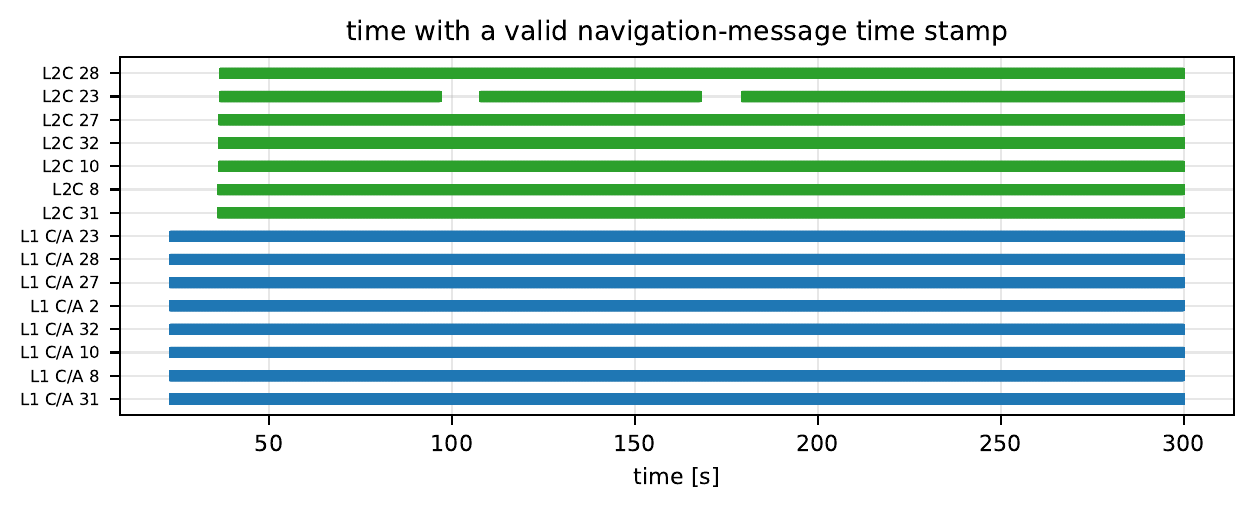
\includegraphics[width=1.0\linewidth]{gnss_sdr/x310_20261022T193000Z/telemetry.png}
  \caption{Telemetry decoder: per band and satellite, when the decoder delivered a valid transmit time (the first one comes after the first complete frame/message).}
\end{figure}

\begin{table}[H]
  \centering
  \footnotesize
  \resizebox{\ifdim\width>\linewidth\linewidth\else\width\fi}{!}{%
  \begin{tabular}{lrrrrr}
    \hline
    \textbf{Band} & \textbf{PRN} & \textbf{Messages decoded} & \textbf{Ephemeris} & \textbf{First valid at [s]} & \textbf{TOW [s]} \\
    \hline
    L1 C/A & 2 & 43 & yes & 23.0 & 415848.0 \\
    L1 C/A & 8 & 47 & yes & 23.0 & 415848.0 \\
    L1 C/A & 10 & 44 & yes & 23.0 & 415848.0 \\
    L1 C/A & 23 & 47 & yes & 23.0 & 415848.0 \\
    L1 C/A & 27 & 43 & yes & 23.0 & 415848.0 \\
    L1 C/A & 28 & 47 & yes & 23.0 & 415848.0 \\
    L1 C/A & 31 & 46 & yes & 29.0 & 415854.0 \\
    L1 C/A & 32 & 44 & yes & 23.0 & 415848.0 \\
    L2C & 8 & 13 & yes & 37.1 & 0.0 \\
    L2C & 10 & 13 & yes & 37.0 & 0.0 \\
    L2C & 23 & 15 & yes & 37.0 & 0.0 \\
    L2C & 27 & 13 & yes & 37.2 & 0.0 \\
    L2C & 28 & 15 & yes & 37.3 & 0.0 \\
    L2C & 31 & 13 & yes & 41.5 & 0.0 \\
    L2C & 32 & 5 & yes & 37.2 & 0.0 \\
    \hline
  \end{tabular}}
  \caption{Telemetry decoder: L1 C/A LNAV subframes and L2C/L5 CNAV messages decoded, ephemeris obtained, and the first valid time of week.}
\end{table}

\subsubsection{Observables}
Pseudorange, carrier phase and Doppler of every channel at common receiver epochs.

\begin{figure}[H]
  \centering
  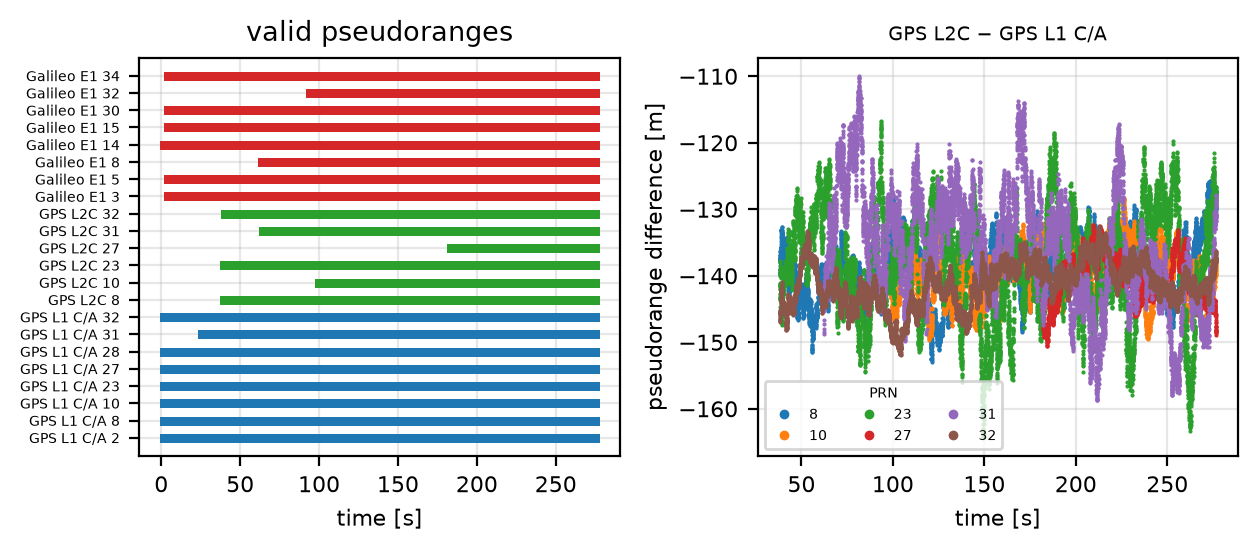
\includegraphics[width=1.0\linewidth]{gnss_sdr/x310_20261022T193000Z/observables.png}
  \caption{Observables: epochs with a valid pseudorange per band and satellite, and the difference between the two bands' pseudoranges of the same satellite (a constant receiver inter-band bias, the same for every satellite, plus the slowly varying ionospheric delay).}
\end{figure}

\begin{table}[H]
  \centering
  \footnotesize
  \resizebox{\ifdim\width>\linewidth\linewidth\else\width\fi}{!}{%
  \begin{tabular}{lrrrrr}
    \hline
    \textbf{PRN} & \textbf{Common epochs} & \textbf{of run [\%]} & \textbf{Mean [m]} & \textbf{Std [m]} & \textbf{Drift [m/s]} \\
    \hline
    8 & 11916 & 80 & -138.80 & 4.22 & 0.0219 \\
    10 & 11920 & 80 & -139.38 & 4.60 & 0.0063 \\
    23 & 11921 & 80 & -138.23 & 7.93 & -0.0050 \\
    27 & 11910 & 79 & -139.78 & 3.33 & -0.0115 \\
    28 & 11906 & 79 & -140.55 & 4.96 & 0.0113 \\
    31 & 11953 & 80 & -135.37 & 8.55 & -0.0633 \\
    32 & 4724 & 32 & -139.80 & 2.42 & -0.0338 \\
    \hline
  \end{tabular}}
  \caption{Observables: P$_{\mathrm{L2C}}$ $-$ P$_{\mathrm{L1}}$ per satellite at common epochs (similar means = shared receiver bias; std = code noise of both bands).}
\end{table}

\subsubsection{PVT}
Position from the pseudoranges and the decoded ephemeris, compared with the surveyed antenna position (-23.209433$^\circ$, -45.874875$^\circ$, 596.42~m).

\begin{figure}[H]
  \centering
  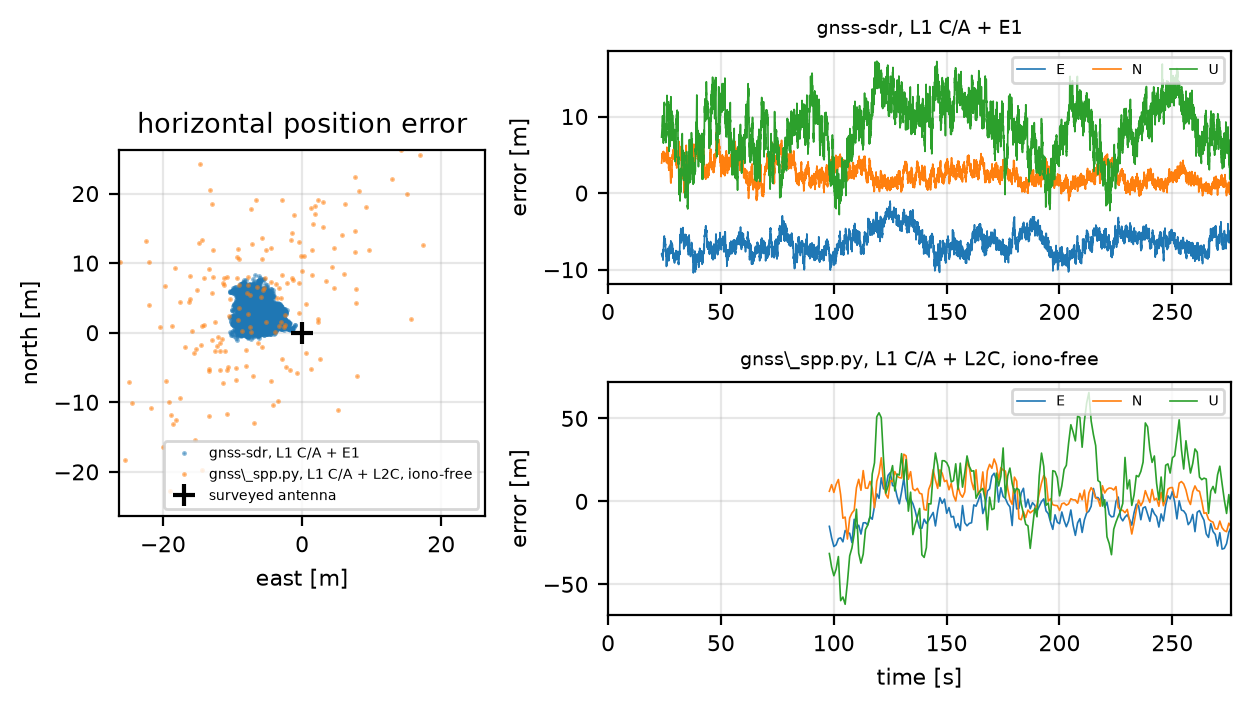
\includegraphics[width=1.0\linewidth]{gnss_sdr/x310_20261022T193000Z/pvt.png}
  \caption{PVT: position error with respect to the surveyed antenna position. L1 C/A: gnss-sdr's own solution (broadcast ionosphere model). Iono-free: computed from gnss-sdr's observables and decoded ephemeris (gnss\_spp.py), removing the ionospheric delay with the second band (pseudoranges carrier-smoothed over 100~s).}
\end{figure}

\begin{figure}[H]
  \centering
  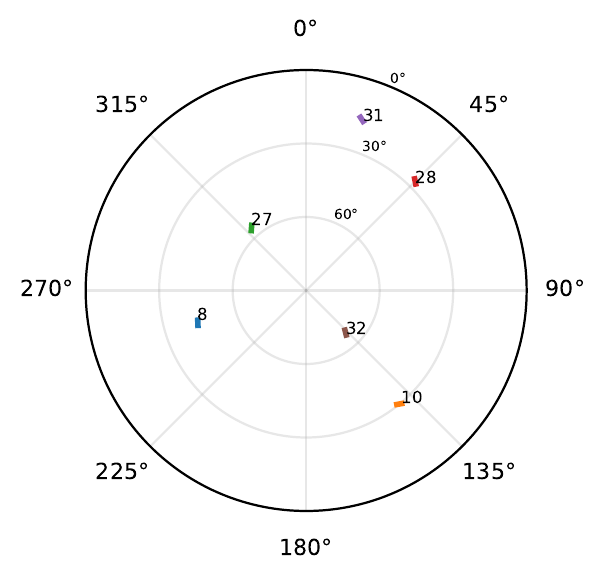
\includegraphics[width=0.45\linewidth]{gnss_sdr/x310_20261022T193000Z/skyplot.png}
  \caption{PVT: sky plot of the satellites in the dual-frequency solution (azimuth, elevation) during the recording.}
\end{figure}

\begin{table}[H]
  \centering
  \footnotesize
  \resizebox{\ifdim\width>\linewidth\linewidth\else\width\fi}{!}{%
  \begin{tabular}{l>{\centering\arraybackslash}p{3.8cm}>{\centering\arraybackslash}p{3.8cm}}
    \hline
    \textbf{Solution} & \textbf{gnss-sdr, L1 C/A} & \textbf{iono-free L1 C/A + L2C} \\
    \hline
    Solutions & 13139 & 238 \\
    Run with fix [\%] & 92 & 86 \\
    Mean E / N / U [m] & -6.3 / 2.8 / 10.0 & -6.9 / 4.4 / 10.4 \\
    Std E / N / U [m] & 1.8 / 1.9 / 4.6 & 8.8 / 7.7 / 25.7 \\
    RMS 2-D [m] & 7.4 & 14.2 \\
    RMS 3-D [m] & 13.3 & 31.2 \\
    95\% horiz. [m] & 10.2 & 25.0 \\
    \hline
  \end{tabular}}
  \caption{PVT: position error statistics with respect to the surveyed antenna (mean = accuracy, std = precision; \% of the run's seconds with a position; gnss-sdr outputs several solutions per second, the iono-free one is computed once per second).}
\end{table}




\section{Records on 23/10/2026}

\subsection{First record}
\begin{table}[H]
  \centering
  \begin{tabular}{|l|l|l|}
    \hline
    \textbf{Parameter} & \textbf{Channel 0} & \textbf{Channel 1} \\
    \hline
    Start time & \multicolumn{2}{>{\centering\arraybackslash}p{7cm}|}{2026-10-23 19:00:06 UTC} \\
    \hline
    Frequency & 1575.420 MHz (L1) & 1176.450 MHz (L5) \\
    \hline
    Duration & 300.0 s & 300.0 s \\
    \hline
    Sample rate & 4.000 MS/s & 20.000 MS/s \\
    \hline
    Sample type & \multicolumn{2}{>{\centering\arraybackslash}p{7cm}|}{signed complex 8-bit samples (I+Q), converted on the host from the X310's sc16} \\
    \hline
    Gain & 25.0 dB & 25.0 dB \\
    \hline
    Antenna & RX1 & RX2 \\
    \hline
    File size & 2400.0 MB & 12000.0 MB \\
    \hline
    Samples written & 1,200,000,000 & 6,000,000,000 \\
    \hline
    Lost samples & 0 & 0 \\
    \hline
    Clock source & \multicolumn{2}{>{\centering\arraybackslash}p{7cm}|}{external} \\
    \hline
    Time source & \multicolumn{2}{>{\centering\arraybackslash}p{7cm}|}{internal} \\
    \hline
    Motherboard & \multicolumn{2}{>{\centering\arraybackslash}p{7cm}|}{USRP X310} \\
    \hline
    Daughterboard & TwinRX RX0 & TwinRX RX1 \\
    \hline
    Recorder & \multicolumn{2}{>{\centering\arraybackslash}p{7cm}|}{UHD Python API} \\
    \hline
    GNSS-SDR configuration & \multicolumn{2}{>{\centering\arraybackslash}p{7cm}|}{\texttt{l1ca8bits4msps\_l5\_8bits20msps.conf}, \texttt{e1\_8bits4msps\_e5a\_8bits20msps.conf}} \\
    \hline
  \end{tabular}
  \caption{Metadata for recording \texttt{x310\_20261023T190000Z}, captured starting 2026-10-23T19:00:06.932068Z.}
\end{table}

\subsubsection{Signal source}
Raw I/Q samples of each channel analysed within the window [10, 10.5]~s after the start recording instant.

\begin{figure}[H]
  \centering
  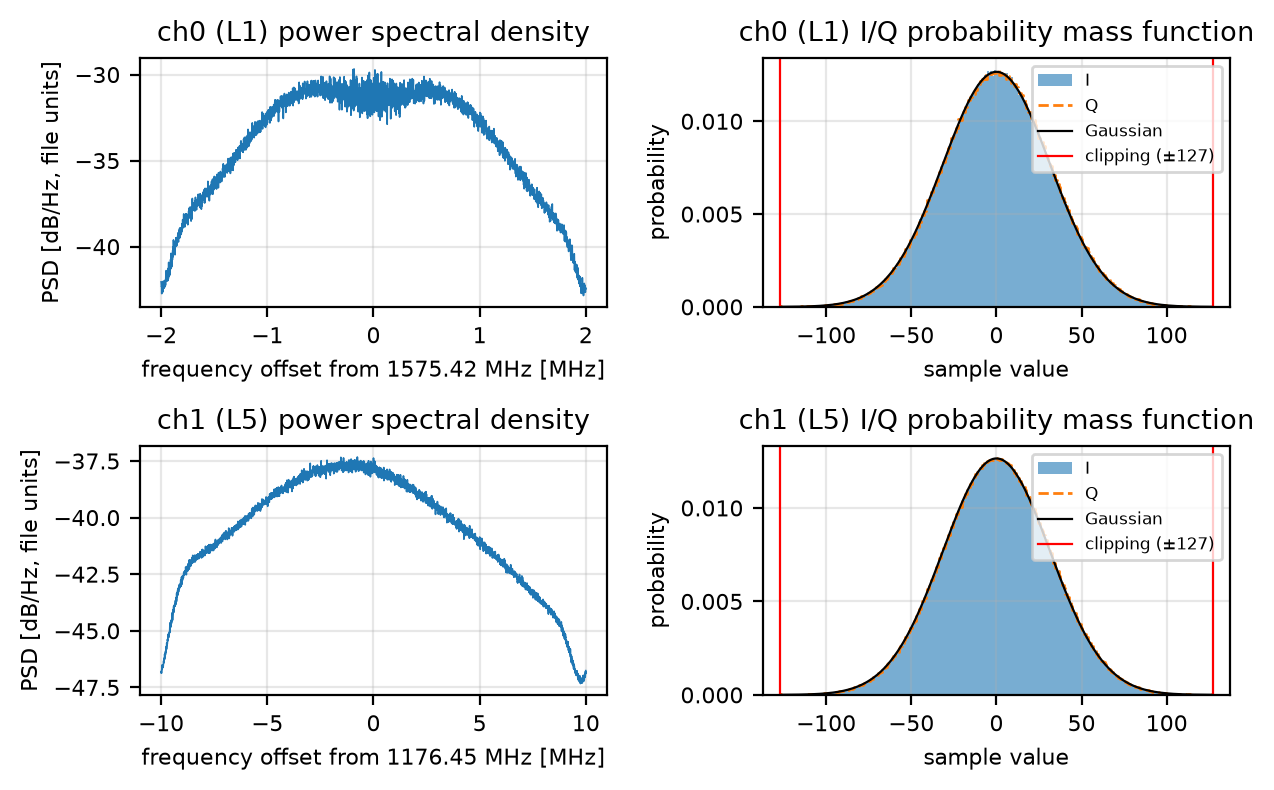
\includegraphics[width=1.0\linewidth]{gnss_sdr/x310_20261023T190000Z/source.png}
  \caption{Signal source: power spectral density (the receiver passband over a flat thermal-noise floor; GNSS signals are below the noise, so only interference would stand out) and probability mass functions of the integer I/Q sample values (Gaussian noise, centred, not clipped).}
\end{figure}

\begin{table}[H]
  \centering
  \footnotesize
  \resizebox{\ifdim\width>\linewidth\linewidth\else\width\fi}{!}{%
  \begin{tabular}{l>{\centering\arraybackslash}p{4.2cm}>{\centering\arraybackslash}p{4.2cm}}
    \hline
    \textbf{Channel} & \textbf{ch0} & \textbf{ch1} \\
    \hline
    Frequency [MHz] & 1575.42 & 1176.45 \\
    Rate [MS/s] & 4 & 20 \\
    Format & ci8 & ci8 \\
    Bytes per complex sample & 2 (1 for I, 1 for Q) & 2 (1 for I, 1 for Q) \\
    Full scale & $\pm$127 & $\pm$127 \\
    Gain [dB] & 25 & 25 \\
    Std I / Q & 31.5 / 31.5 & 31.5 / 31.5 \\
    Mean I / Q & 0.04 / 0.07 & 0.04 / 0.01 \\
    Min / max I & -127 / 127 & -127 / 127 \\
    Min / max Q & -127 / 127 & -127 / 127 \\
    Headroom\footnotemark & 4.0 & 4.0 \\
    Clipped [\%] & 0.006 & 0.006 \\
    Lost samples & 0 & 0 \\
    \hline
  \end{tabular}}
  \caption{Signal source: sample statistics per channel (headroom: how many standard deviations of the noise fit before clipping).}
\end{table}

\footnotetext{Headroom $= A/\sigma$, where $A$ is the full scale of the sample format (127 for 8-bit, 32767 for 16-bit) and $\sigma$ the standard deviation of the I and Q samples together (both in file units, over the analysed window). For Gaussian noise, the fraction of clipped values is $2Q(A/\sigma)$, with $Q$ the Gaussian tail function: e.g. 0.003\,\% at $4.2\sigma$.}

\subsubsection{Signal conditioner}


\begin{table}[H]
  \centering
  \footnotesize
  \resizebox{\ifdim\width>\linewidth\linewidth\else\width\fi}{!}{%
  \begin{tabular}{l>{\centering\arraybackslash}p{4.2cm}>{\centering\arraybackslash}p{4.2cm}}
    \hline
    \textbf{Channel} & \textbf{ch0 (L1 C/A)} & \textbf{ch1 (L5)} \\
    \hline
    File format & ci8 & ci8 \\
    Source item type & ibyte & ibyte \\
    Data type adapter & Ibyte\_To\_Complex & Ibyte\_To\_Complex \\
    Input filter & Pass\_Through & Pass\_Through \\
    Resampling & $\times$5 zero-order hold, offline (\texttt{upsample\_iq.py}) & Pass\_Through \\
    Rate [MS/s] & 4 $\to$ 20 & 20 $\to$ 20 \\
    \hline
  \end{tabular}}
  \caption{Signal conditioner: recorded format and rate to gnss-sdr's internal \texttt{gr\_complex} stream; both bands are read in lockstep by one \texttt{Multichannel\_File\_Signal\_Source}.}
\end{table}

\subsubsection{Acquisition}
Two-dimensional search over code delay and Doppler (one channel per band dumped; the others behave alike).

\begin{figure}[H]
  \centering
  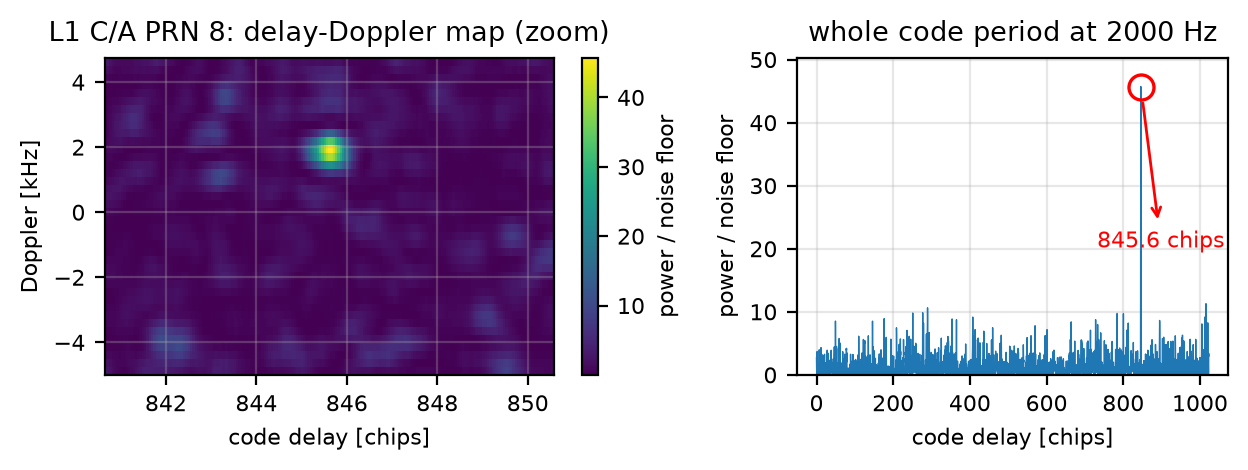
\includegraphics[width=1.0\linewidth]{gnss_sdr/x310_20261023T190000Z/acq_1C.png}
  \caption{Acquisition, L1 C/A: delay--Doppler search of PRN 8; one sharp peak (test statistic 59 vs threshold 47) at 2000~Hz and 845.6~chips.}
\end{figure}

\begin{figure}[H]
  \centering
  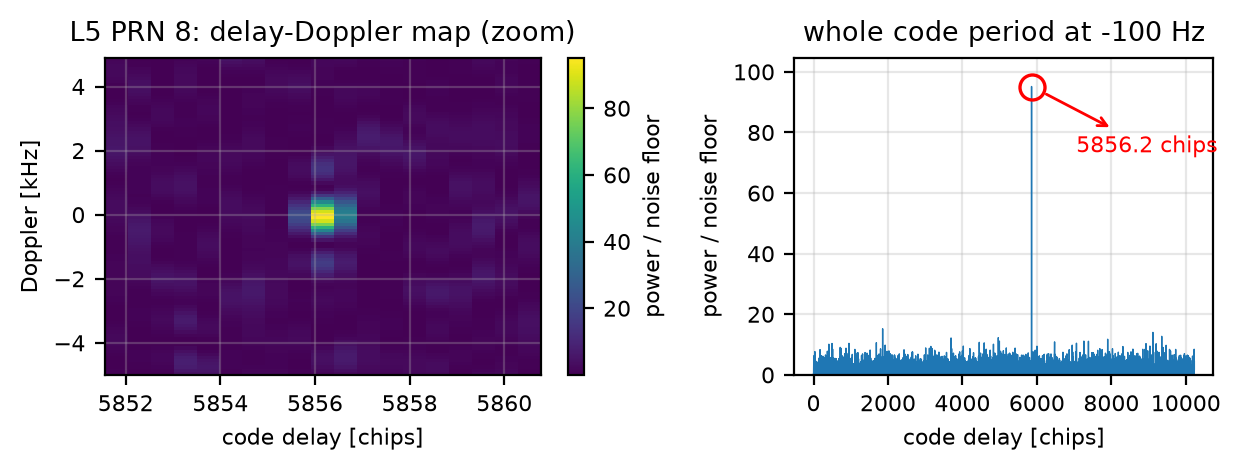
\includegraphics[width=1.0\linewidth]{gnss_sdr/x310_20261023T190000Z/acq_L5.png}
  \caption{Acquisition, L5: delay--Doppler search of PRN 8; one sharp peak (test statistic 134 vs threshold 49) at 1392~Hz and 5856.2~chips.}
\end{figure}

\begin{table}[H]
  \centering
  \footnotesize
  \resizebox{\ifdim\width>\linewidth\linewidth\else\width\fi}{!}{%
  \begin{tabular}{lrrrr}
    \hline
    \textbf{Band} & \textbf{Attempts} & \textbf{Detections} & \textbf{Detected PRNs} & \textbf{Best statistic / threshold\footnotemark} \\
    \hline
    L1 C/A & 6 & 1 & 8 & 1.2 \\
    L5 & 2 & 2 & 8 & 2.7 \\
    \hline
  \end{tabular}}
  \caption{Acquisition: search attempts of the dumped channel. Attempts on satellites that are not in view (or do not broadcast that signal, e.g. older GPS satellites on L5/L2C) are rejected below the threshold.}
\end{table}

\footnotetext{Margin of the band's strongest detection: the largest acquisition test statistic among the detected attempts (the correlation peak of the delay--Doppler grid, normalised by the power of the input samples searched, i.e. the noise power, since GNSS signals are below the noise) divided by the detection threshold, which GNSS-SDR derives from the configured probability of false alarm. A value of 1 is right at the detection limit; e.g. 2.5 means the peak cleared the threshold 2.5 times over.}

\subsubsection{Tracking}


\begin{figure}[H]
  \centering
  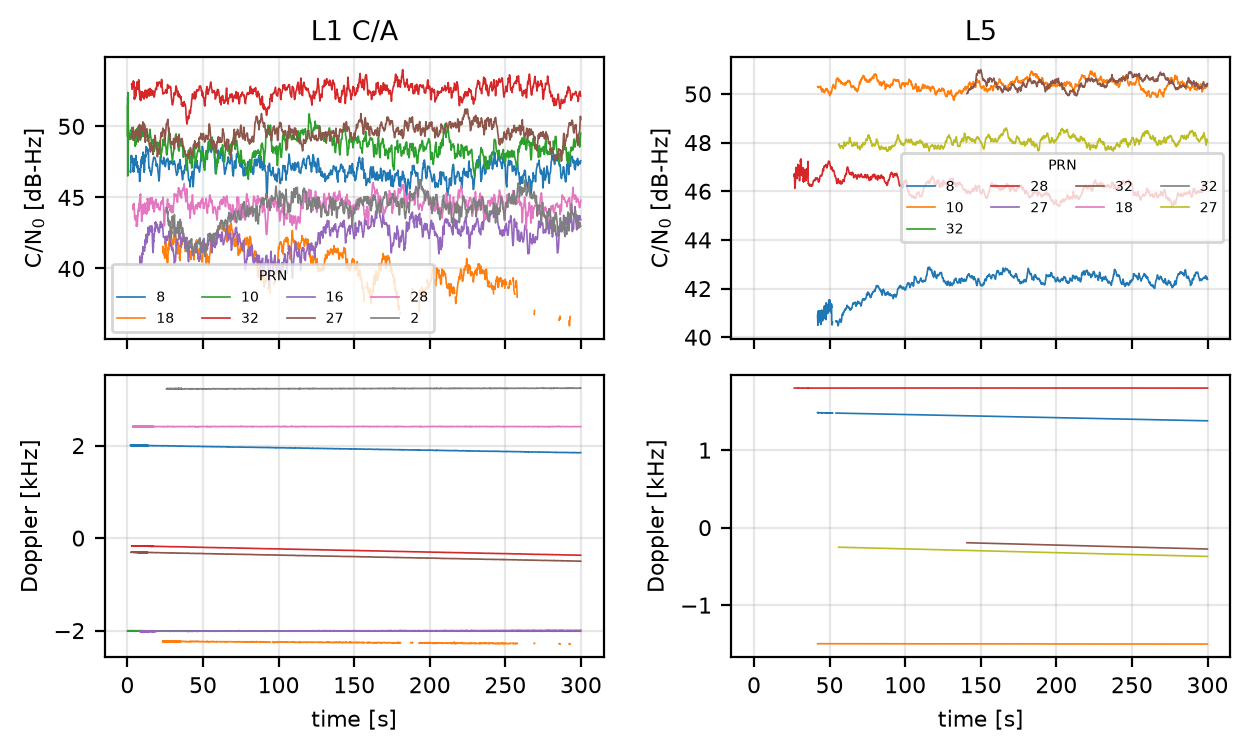
\includegraphics[width=1.0\linewidth]{gnss_sdr/x310_20261023T190000Z/tracking.png}
  \caption{Tracking: carrier-to-noise density ratio and carrier Doppler per satellite, while phase-locked (smooth Doppler curves = loops following the real satellite motion).}
\end{figure}

\begin{figure}[H]
  \centering
  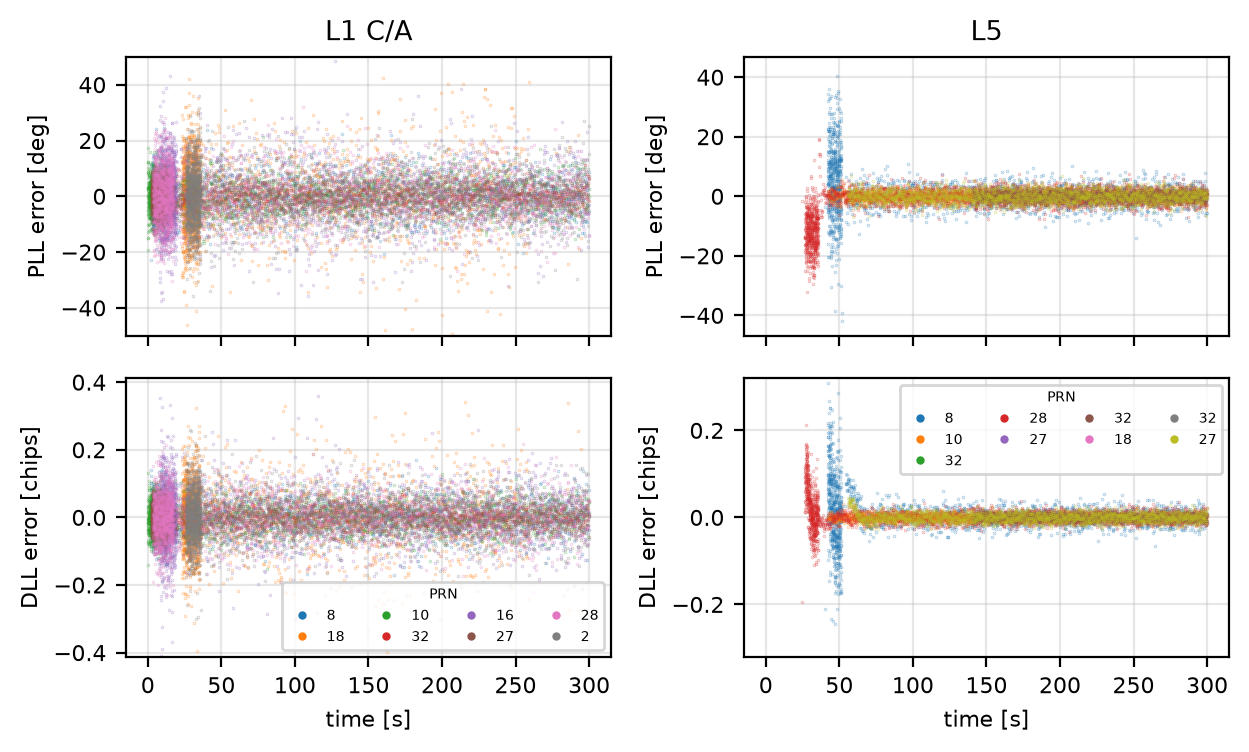
\includegraphics[width=1.0\linewidth]{gnss_sdr/x310_20261023T190000Z/tracking_errors.png}
  \caption{Tracking: loop errors per satellite while phase-locked, i.e. the discriminator outputs that the loops drive to zero: PLL carrier-phase error (degrees) and DLL code-delay error (chips) of every correlation. Noise centred on zero = clean tracking; its spread grows as C/N$_0$ drops, and jumps would mark cycle slips or a loop losing lock.}
\end{figure}

\begin{figure}[H]
  \centering
  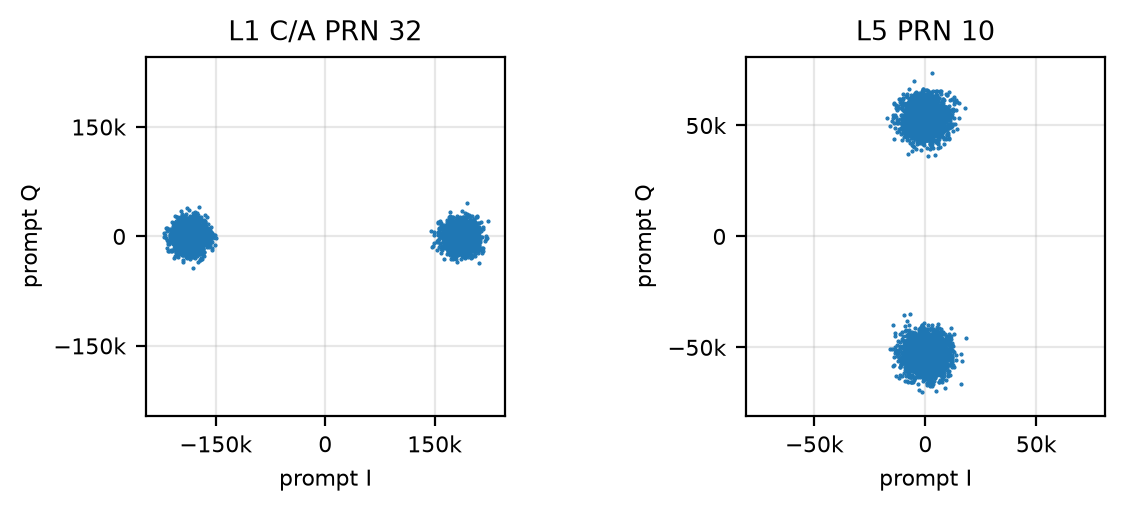
\includegraphics[width=1.0\linewidth]{gnss_sdr/x310_20261023T190000Z/tracking_iq.png}
  \caption{Tracking: prompt correlator outputs of the strongest satellite per band. Two tight clusters on one axis (the $\pm1$ data bits; GNSS-SDR's L5 tracking puts the data component on the Q axis), or, for the dataless pilots tracked for Galileo (E1-C, E5a-Q), the $\pm1$ chips of their secondary code, mean the PLL is phase-locked; a ring would mean it is not. \texttt{Prompt\_I}/\texttt{Prompt\_Q} are 32-bit floats (sums of the samples over one integration period, in file units): they never clip, only overflowing beyond $\pm 3.4\times10^{38}$, far above the $N\cdot\text{full scale}\cdot\sqrt{2}$ a sum of $N$ samples can reach.}
\end{figure}

\begin{table}[H]
  \centering
  \footnotesize
  \resizebox{\ifdim\width>\linewidth\linewidth\else\width\fi}{!}{%
  \begin{tabular}{lrrrrrrrr}
    \hline
    \textbf{Band} & \textbf{Ch.} & \textbf{PRN} & \textbf{Median C/N$_0$ [dB-Hz]} & \textbf{Phase-locked [\%]} & \textbf{Losses of lock} & \textbf{Tracked [s]} & \textbf{PLL error std [deg]} & \textbf{DLL error std [chips]} \\
    \hline
    L1 C/A & 0 & 8 & 47.2 & 99 & 0 & 298 & 6.3 & 0.048 \\
    L1 C/A & 1 & 18 & 41.1 & 86 & 0 & 277 & 13.2 & 0.099 \\
    L1 C/A & 2 & 10 & 49.1 & 100 & 0 & 300 & 5.2 & 0.038 \\
    L1 C/A & 3 & 32 & 52.4 & 95 & 0 & 299 & 3.5 & 0.025 \\
    L1 C/A & 4 & 16 & 42.3 & 95 & 0 & 293 & 11.1 & 0.085 \\
    L1 C/A & 5 & 27 & 49.5 & 95 & 0 & 299 & 4.8 & 0.036 \\
    L1 C/A & 6 & 28 & 44.4 & 91 & 0 & 299 & 8.9 & 0.063 \\
    L1 C/A & 7 & 2 & 43.6 & 96 & 0 & 275 & 9.5 & 0.068 \\
    L5 & 8 & 8 & 41.2 & 66 & 1 & 276 & 7.8 & 0.052 \\
    L5 & 9 & 10 & 50.4 & 68 & 0 & 282 & 1.5 & 0.007 \\
    L5 & 10 & 32 & 29.1 & 0 & 2 & 32 & -- & -- \\
    L5 & 11 & 28 & 46.3 & 95 & 0 & 275 & 6.7 & 0.032 \\
    L5 & 13 & 27 & 28.9 & 0 & 3 & 16 & -- & -- \\
    L5 & 13 & 32 & 47.7 & 29 & 3 & 210 & 1.5 & 0.007 \\
    L5 & 14 & 18 & 28.6 & 0 & 3 & 16 & -- & -- \\
    L5 & 14 & 32 & 29.0 & 0 & 3 & 32 & -- & -- \\
    L5 & 15 & 27 & 48.0 & 68 & 0 & 260 & 1.9 & 0.010 \\
    \hline
  \end{tabular}}
  \caption{Tracking: per channel and satellite (phase-locked: carrier lock test $> 0.8$; loop error standard deviations while phase-locked).}
\end{table}

\subsubsection{Telemetry decoder}


\begin{figure}[H]
  \centering
  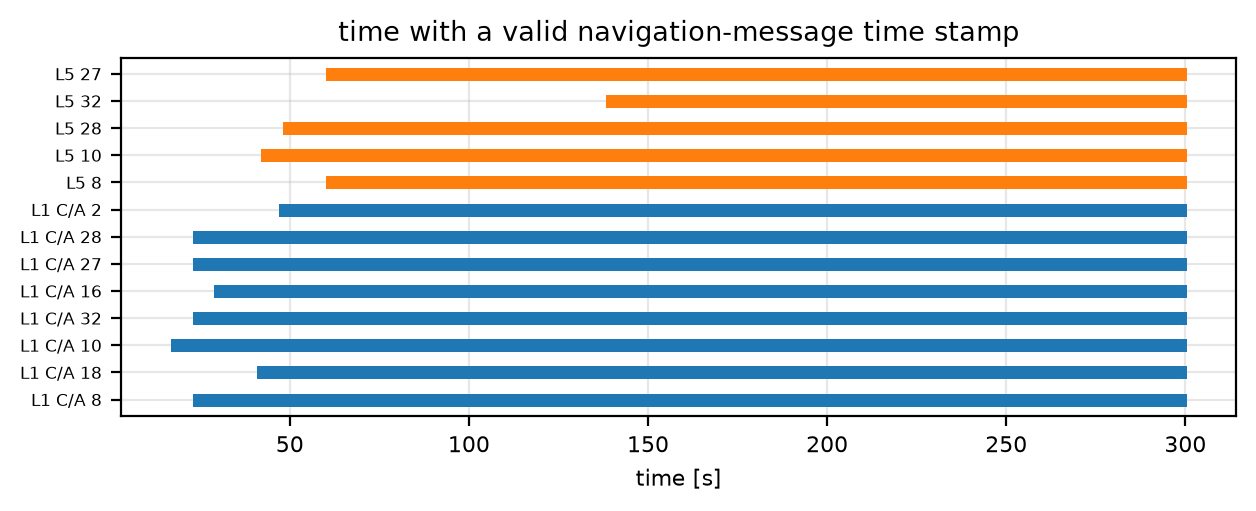
\includegraphics[width=1.0\linewidth]{gnss_sdr/x310_20261023T190000Z/telemetry.png}
  \caption{Telemetry decoder: per band and satellite, when the decoder delivered a valid transmit time (the first one comes after the first complete frame/message).}
\end{figure}

\begin{table}[H]
  \centering
  \footnotesize
  \resizebox{\ifdim\width>\linewidth\linewidth\else\width\fi}{!}{%
  \begin{tabular}{lrrrrr}
    \hline
    \textbf{Band} & \textbf{PRN} & \textbf{Messages decoded} & \textbf{Ephemeris} & \textbf{First valid at [s]} & \textbf{TOW [s]} \\
    \hline
    L1 C/A & 2 & 43 & yes & 47.1 & 500472.0 \\
    L1 C/A & 8 & 47 & yes & 23.1 & 500448.0 \\
    L1 C/A & 10 & 48 & yes & 17.1 & 500442.0 \\
    L1 C/A & 16 & 46 & yes & 29.1 & 500454.0 \\
    L1 C/A & 18 & 44 & yes & 41.2 & 500466.0 \\
    L1 C/A & 27 & 47 & yes & 23.1 & 500448.0 \\
    L1 C/A & 28 & 47 & yes & 23.1 & 500448.0 \\
    L1 C/A & 32 & 47 & yes & 23.1 & 500448.0 \\
    L5 & 8 & 25 & yes & 60.3 & 500485.1 \\
    L5 & 10 & 26 & yes & 42.1 & 500467.0 \\
    L5 & 27 & 25 & yes & 60.3 & 500485.2 \\
    L5 & 28 & 32 & yes & 48.4 & 500473.3 \\
    L5 & 32 & 16 & yes & 138.5 & 500563.3 \\
    \hline
  \end{tabular}}
  \caption{Telemetry decoder: L1 C/A LNAV subframes, L5 CNAV messages decoded, ephemeris obtained, and the first valid time of week.}
\end{table}

\subsubsection{Observables}
Pseudorange, carrier phase and Doppler of every channel at common receiver epochs.

\begin{figure}[H]
  \centering
  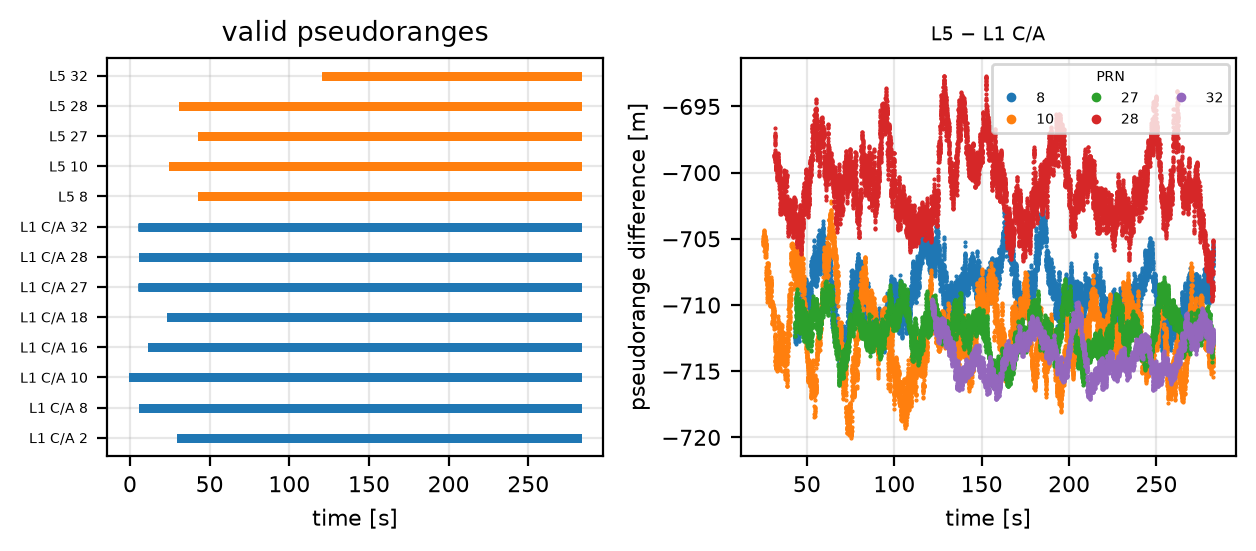
\includegraphics[width=1.0\linewidth]{gnss_sdr/x310_20261023T190000Z/observables.png}
  \caption{Observables: epochs with a valid pseudorange per band and satellite, and the difference between the two bands' pseudoranges of the same satellite (a constant receiver inter-band bias, the same for every satellite, plus the slowly varying ionospheric delay).}
\end{figure}

\begin{table}[H]
  \centering
  \footnotesize
  \resizebox{\ifdim\width>\linewidth\linewidth\else\width\fi}{!}{%
  \begin{tabular}{lrrrrrr}
    \hline
    \textbf{Difference} & \textbf{PRN} & \textbf{Common epochs} & \textbf{of run [\%]} & \textbf{Mean [m]} & \textbf{Std [m]} & \textbf{Drift [m/s]} \\
    \hline
    L5 $-$ L1 C/A & 8 & 11972 & 80 & -709.04 & 2.07 & -0.0001 \\
    L5 $-$ L1 C/A & 10 & 12837 & 86 & -712.22 & 2.77 & -0.0056 \\
    L5 $-$ L1 C/A & 27 & 11970 & 80 & -711.92 & 1.52 & -0.0025 \\
    L5 $-$ L1 C/A & 28 & 12563 & 84 & -700.94 & 2.75 & -0.0052 \\
    L5 $-$ L1 C/A & 32 & 8062 & 54 & -713.71 & 1.50 & 0.0021 \\
    \hline
  \end{tabular}}
  \caption{Observables: pseudorange difference between the two bands of each satellite at common epochs (similar means = shared receiver bias; std = code noise of both bands).}
\end{table}

\subsubsection{PVT}
Position from the pseudoranges and the decoded ephemeris, compared with the surveyed antenna position (-23.209433$^\circ$, -45.874875$^\circ$, 596.42~m).

\begin{figure}[H]
  \centering
  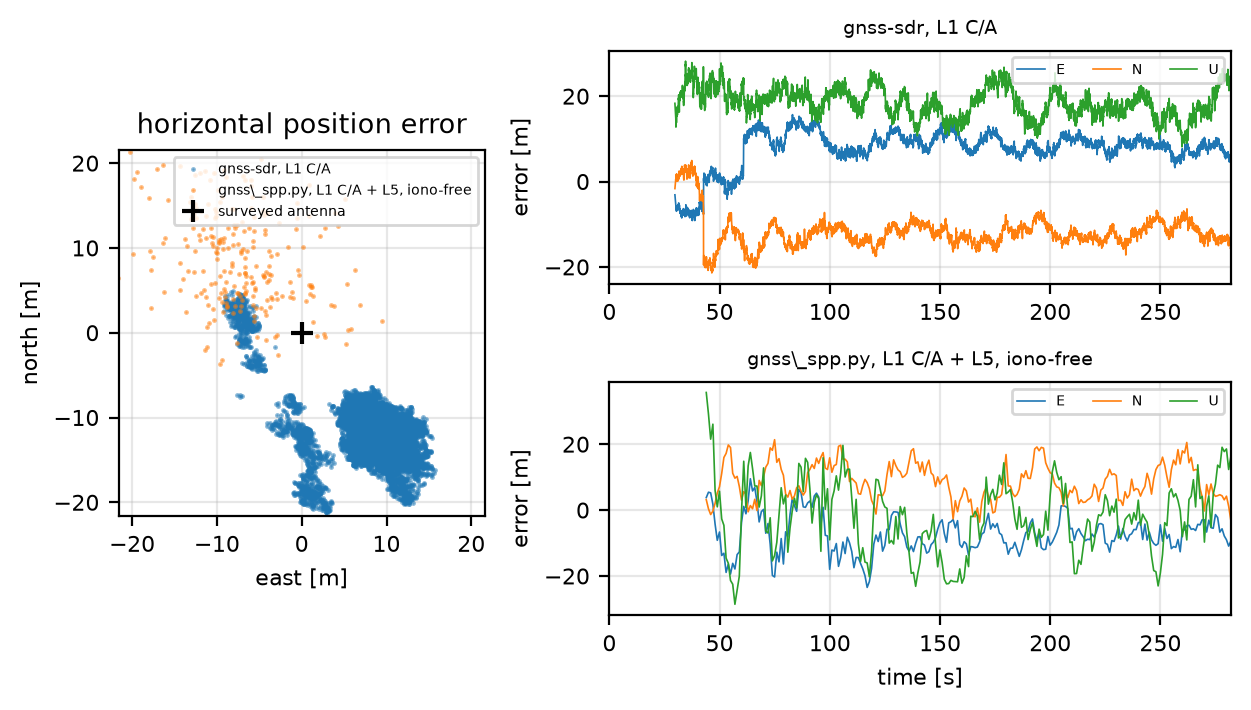
\includegraphics[width=1.0\linewidth]{gnss_sdr/x310_20261023T190000Z/pvt.png}
  \caption{PVT: position error with respect to the surveyed antenna position. gnss-sdr: GNSS-SDR's own RTKLIB solution (single frequency, broadcast ionosphere model). gnss\_spp\_lib.py: computed from gnss-sdr's observables and decoded GPS ephemeris, removing the ionospheric delay with the second band (pseudoranges carrier-smoothed over 100~s).}
\end{figure}

\begin{figure}[H]
  \centering
  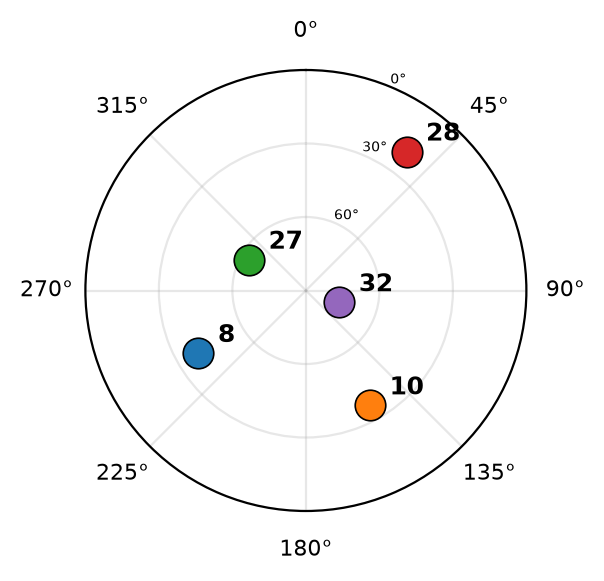
\includegraphics[width=0.45\linewidth]{gnss_sdr/x310_20261023T190000Z/skyplot.png}
  \caption{PVT: sky plot of the GPS satellites in the gnss\_spp\_lib.py dual-frequency solution (azimuth, elevation) during the recording.}
\end{figure}

\begin{table}[H]
  \centering
  \footnotesize
  \resizebox{\ifdim\width>\linewidth\linewidth\else\width\fi}{!}{%
  \begin{tabular}{l>{\centering\arraybackslash}p{4.2cm}>{\centering\arraybackslash}p{4.2cm}}
    \hline
    \textbf{Solution} & \textbf{gnss-sdr, L1 C/A} & \textbf{gnss\_spp\_lib.py, L1 C/A + L5, iono-free} \\
    \hline
    Solutions & 13133 & 239 \\
    Run with fix [\%] & 90 & 85 \\
    Mean E / N / U [m] & 7.7 / -11.8 / 18.5 & -7.3 / 8.5 / -2.1 \\
    Std E / N / U [m] & 4.5 / 3.8 / 3.5 & 5.7 / 5.5 / 11.1 \\
    RMS 2-D [m] & 15.3 & 13.8 \\
    RMS 3-D [m] & 24.3 & 17.8 \\
    95\% horiz. [m] & 20.1 & 22.2 \\
    \hline
  \end{tabular}}
  \caption{PVT: position error statistics with respect to the surveyed antenna (mean = accuracy, std = precision; \% of the run's seconds with a position; gnss-sdr outputs several solutions per second, gnss\_spp\_lib.py computes one per second).}
\end{table}


\subsubsection{Signal conditioner}


\begin{table}[H]
  \centering
  \footnotesize
  \resizebox{\ifdim\width>\linewidth\linewidth\else\width\fi}{!}{%
  \begin{tabular}{l>{\centering\arraybackslash}p{4.2cm}>{\centering\arraybackslash}p{4.2cm}}
    \hline
    \textbf{Channel} & \textbf{ch0 (E1)} & \textbf{ch1 (E5a)} \\
    \hline
    File format & ci8 & ci8 \\
    Source item type & ibyte & ibyte \\
    Data type adapter & Ibyte\_To\_Complex & Ibyte\_To\_Complex \\
    Input filter & Pass\_Through & Pass\_Through \\
    Resampling & $\times$5 zero-order hold, offline (\texttt{upsample\_iq.py}) & Pass\_Through \\
    Rate [MS/s] & 4 $\to$ 20 & 20 $\to$ 20 \\
    \hline
  \end{tabular}}
  \caption{Signal conditioner: recorded format and rate to gnss-sdr's internal \texttt{gr\_complex} stream; both bands are read in lockstep by one \texttt{Multichannel\_File\_Signal\_Source}.}
\end{table}

\subsubsection{Acquisition}
Two-dimensional search over code delay and Doppler (one channel per band dumped; the others behave alike).

\begin{figure}[H]
  \centering
  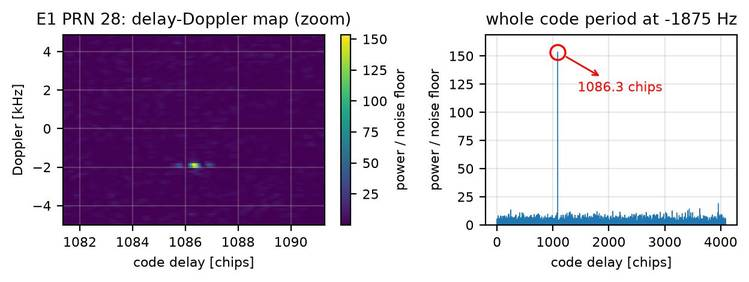
\includegraphics[width=1.0\linewidth]{gnss_sdr/x310_20261023T190000Z/galileo_acq_1B.jpg}
  \caption{Acquisition, E1: delay--Doppler search of PRN 28; one sharp peak (test statistic 215 vs threshold 52) at -1875~Hz and 1086.3~chips.}
\end{figure}

\begin{figure}[H]
  \centering
  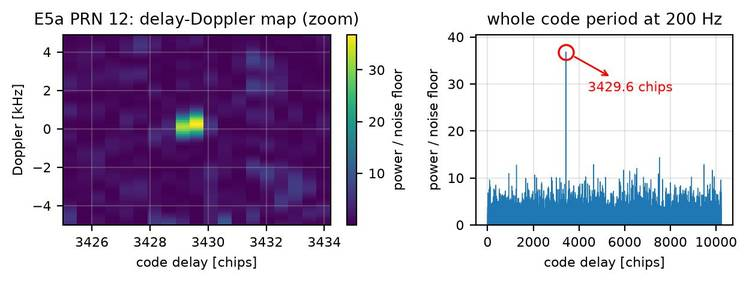
\includegraphics[width=1.0\linewidth]{gnss_sdr/x310_20261023T190000Z/galileo_acq_5X.jpg}
  \caption{Acquisition, E5a: delay--Doppler search of PRN 12; one sharp peak (test statistic 51 vs threshold 49) at -492~Hz and 3429.6~chips.}
\end{figure}

\begin{table}[H]
  \centering
  \footnotesize
  \resizebox{\ifdim\width>\linewidth\linewidth\else\width\fi}{!}{%
  \begin{tabular}{lrrrr}
    \hline
    \textbf{Band} & \textbf{Attempts} & \textbf{Detections} & \textbf{Detected PRNs} & \textbf{Best statistic / threshold\footnotemark} \\
    \hline
    E1 & 9 & 4 & 28 & 4.1 \\
    E5a & 2 & 1 & 12 & 1.0 \\
    \hline
  \end{tabular}}
  \caption{Acquisition: search attempts of the dumped channel. Attempts on satellites that are not in view (or do not broadcast that signal, e.g. older GPS satellites on L5/L2C) are rejected below the threshold.}
\end{table}

\footnotetext{Margin of the band's strongest detection: the largest acquisition test statistic among the detected attempts (the correlation peak of the delay--Doppler grid, normalised by the power of the input samples searched, i.e. the noise power, since GNSS signals are below the noise) divided by the detection threshold, which GNSS-SDR derives from the configured probability of false alarm. A value of 1 is right at the detection limit; e.g. 2.5 means the peak cleared the threshold 2.5 times over.}

\subsubsection{Tracking}


\begin{figure}[H]
  \centering
  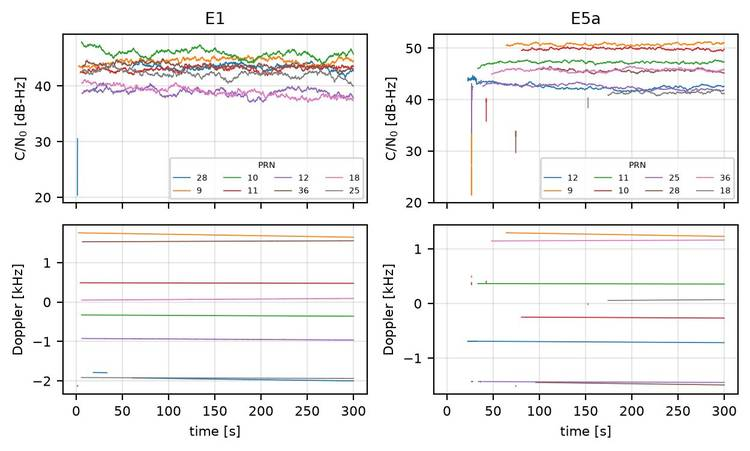
\includegraphics[width=1.0\linewidth]{gnss_sdr/x310_20261023T190000Z/galileo_tracking.jpg}
  \caption{Tracking: carrier-to-noise density ratio and carrier Doppler per satellite, while phase-locked (smooth Doppler curves = loops following the real satellite motion).}
\end{figure}

\begin{figure}[H]
  \centering
  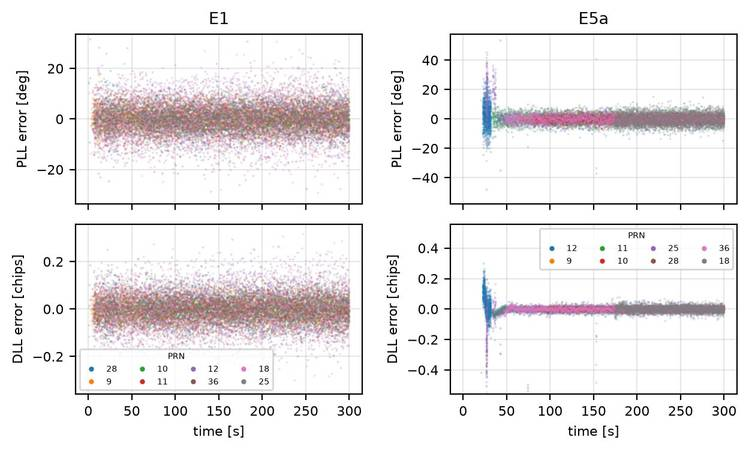
\includegraphics[width=1.0\linewidth]{gnss_sdr/x310_20261023T190000Z/galileo_tracking_errors.jpg}
  \caption{Tracking: loop errors per satellite while phase-locked, i.e. the discriminator outputs that the loops drive to zero: PLL carrier-phase error (degrees) and DLL code-delay error (chips) of every correlation. Noise centred on zero = clean tracking; its spread grows as C/N$_0$ drops, and jumps would mark cycle slips or a loop losing lock.}
\end{figure}

\begin{figure}[H]
  \centering
  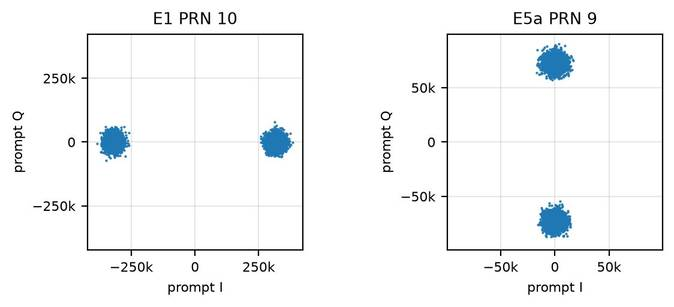
\includegraphics[width=1.0\linewidth]{gnss_sdr/x310_20261023T190000Z/galileo_tracking_iq.jpg}
  \caption{Tracking: prompt correlator outputs of the strongest satellite per band. Two tight clusters on one axis (the $\pm1$ data bits; GNSS-SDR's L5 tracking puts the data component on the Q axis), or, for the dataless pilots tracked for Galileo (E1-C, E5a-Q), the $\pm1$ chips of their secondary code, mean the PLL is phase-locked; a ring would mean it is not. \texttt{Prompt\_I}/\texttt{Prompt\_Q} are 32-bit floats (sums of the samples over one integration period, in file units): they never clip, only overflowing beyond $\pm 3.4\times10^{38}$, far above the $N\cdot\text{full scale}\cdot\sqrt{2}$ a sum of $N$ samples can reach.}
\end{figure}

\begin{table}[H]
  \centering
  \footnotesize
  \resizebox{\ifdim\width>\linewidth\linewidth\else\width\fi}{!}{%
  \begin{tabular}{lrrrrrrrr}
    \hline
    \textbf{Band} & \textbf{Ch.} & \textbf{PRN} & \textbf{Median C/N$_0$ [dB-Hz]} & \textbf{Phase-locked [\%]} & \textbf{Losses of lock} & \textbf{Tracked [s]} & \textbf{PLL error std [deg]} & \textbf{DLL error std [chips]} \\
    \hline
    E1 & 0 & 28 & 43.4 & 85 & 3 & 299 & 5.2 & 0.052 \\
    E1 & 1 & 9 & 44.6 & 99 & 0 & 300 & 4.2 & 0.044 \\
    E1 & 2 & 10 & 45.9 & 98 & 0 & 300 & 3.9 & 0.041 \\
    E1 & 3 & 11 & 43.1 & 99 & 0 & 300 & 5.5 & 0.053 \\
    E1 & 4 & 12 & 39.0 & 98 & 0 & 300 & 8.2 & 0.088 \\
    E1 & 5 & 36 & 43.6 & 98 & 0 & 298 & 4.8 & 0.052 \\
    E1 & 6 & 18 & 39.0 & 98 & 0 & 299 & 8.4 & 0.089 \\
    E1 & 7 & 25 & 42.2 & 98 & 0 & 299 & 5.8 & 0.062 \\
    E5a & 8 & 12 & 42.9 & 92 & 0 & 279 & 6.5 & 0.054 \\
    E5a & 9 & 9 & 50.4 & 30 & 1 & 273 & 4.6 & 0.023 \\
    E5a & 10 & 11 & 47.0 & 54 & 0 & 280 & 3.6 & 0.014 \\
    E5a & 11 & 10 & 29.8 & 20 & 2 & 273 & 3.6 & 0.013 \\
    E5a & 12 & 25 & 42.9 & 60 & 0 & 273 & 7.3 & 0.069 \\
    E5a & 13 & 28 & 45.7 & 47 & 0 & 226 & 3.4 & 0.024 \\
    E5a & 14 & 36 & 45.4 & 52 & 0 & 273 & 2.4 & 0.012 \\
    E5a & 15 & 18 & 41.2 & 35 & 0 & 147 & 4.7 & 0.025 \\
    \hline
  \end{tabular}}
  \caption{Tracking: per channel and satellite (phase-locked: carrier lock test $> 0.8$; loop error standard deviations while phase-locked).}
\end{table}

\subsubsection{Telemetry decoder}


\begin{figure}[H]
  \centering
  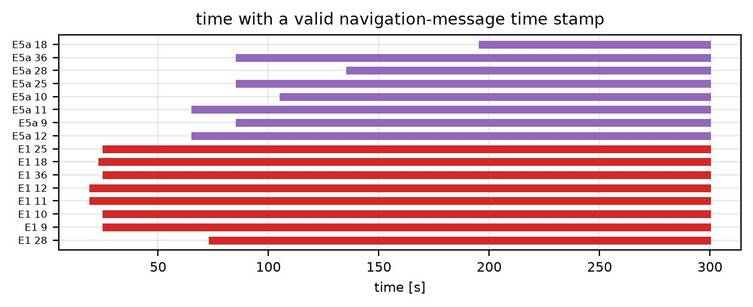
\includegraphics[width=1.0\linewidth]{gnss_sdr/x310_20261023T190000Z/galileo_telemetry.jpg}
  \caption{Telemetry decoder: per band and satellite, when the decoder delivered a valid transmit time (the first one comes after the first complete frame/message).}
\end{figure}

\begin{table}[H]
  \centering
  \footnotesize
  \resizebox{\ifdim\width>\linewidth\linewidth\else\width\fi}{!}{%
  \begin{tabular}{lrrrrr}
    \hline
    \textbf{Band} & \textbf{PRN} & \textbf{Messages decoded} & \textbf{Ephemeris} & \textbf{First valid at [s]} & \textbf{TOW [s]} \\
    \hline
    E1 & 9 & 26 & yes & 25.2 & 500450.0 \\
    E1 & 10 & 27 & yes & 25.2 & 500450.0 \\
    E1 & 11 & 27 & yes & 19.2 & 500444.0 \\
    E1 & 12 & 27 & yes & 19.2 & 500444.0 \\
    E1 & 18 & 26 & yes & 23.2 & 500448.0 \\
    E1 & 25 & 26 & yes & 25.2 & 500450.0 \\
    E1 & 28 & 22 & yes & 73.2 & 500498.0 \\
    E1 & 36 & 27 & yes & 25.2 & 500450.0 \\
    E5a & 9 & 12 & yes & 85.4 & 500510.3 \\
    E5a & 10 & 11 & yes & 105.4 & 500530.3 \\
    E5a & 11 & 13 & yes & 65.4 & 500490.3 \\
    E5a & 12 & 13 & yes & 65.4 & 500490.3 \\
    E5a & 18 & 4 & yes & 195.4 & 500620.3 \\
    E5a & 25 & 12 & yes & 85.4 & 500510.3 \\
    E5a & 28 & 9 & yes & 135.4 & 500560.3 \\
    E5a & 36 & 12 & yes & 85.4 & 500510.3 \\
    \hline
  \end{tabular}}
  \caption{Telemetry decoder: E1 I/NAV words, E5a F/NAV pages decoded, ephemeris obtained, and the first valid time of week.}
\end{table}

\subsubsection{Observables}
Pseudorange, carrier phase and Doppler of every channel at common receiver epochs.

\begin{figure}[H]
  \centering
  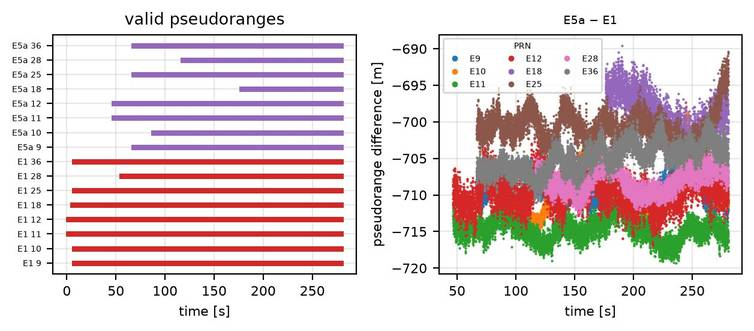
\includegraphics[width=1.0\linewidth]{gnss_sdr/x310_20261023T190000Z/galileo_observables.jpg}
  \caption{Observables: epochs with a valid pseudorange per band and satellite, and the difference between the two bands' pseudoranges of the same satellite (a constant receiver inter-band bias, the same for every satellite, plus the slowly varying ionospheric delay).}
\end{figure}

\begin{table}[H]
  \centering
  \footnotesize
  \resizebox{\ifdim\width>\linewidth\linewidth\else\width\fi}{!}{%
  \begin{tabular}{lrrrrrr}
    \hline
    \textbf{Difference} & \textbf{PRN} & \textbf{Common epochs} & \textbf{of run [\%]} & \textbf{Mean [m]} & \textbf{Std [m]} & \textbf{Drift [m/s]} \\
    \hline
    E5a $-$ E1 & 9 & 10631 & 71 & -709.38 & 1.88 & -0.0007 \\
    E5a $-$ E1 & 10 & 9645 & 64 & -709.26 & 3.55 & 0.0208 \\
    E5a $-$ E1 & 11 & 11505 & 77 & -714.67 & 1.53 & -0.0035 \\
    E5a $-$ E1 & 12 & 11520 & 77 & -709.41 & 2.18 & 0.0012 \\
    E5a $-$ E1 & 18 & 5144 & 34 & -698.88 & 2.95 & -0.0589 \\
    E5a $-$ E1 & 25 & 10637 & 71 & -700.71 & 2.13 & 0.0007 \\
    E5a $-$ E1 & 28 & 8150 & 54 & -708.06 & 1.63 & 0.0079 \\
    E5a $-$ E1 & 36 & 10632 & 71 & -704.86 & 1.92 & 0.0213 \\
    \hline
  \end{tabular}}
  \caption{Observables: pseudorange difference between the two bands of each satellite at common epochs (similar means = shared receiver bias; std = code noise of both bands).}
\end{table}

\subsubsection{PVT}
Position from the pseudoranges and the decoded ephemeris, compared with the surveyed antenna position (-23.209433$^\circ$, -45.874875$^\circ$, 596.42~m).

\begin{figure}[H]
  \centering
  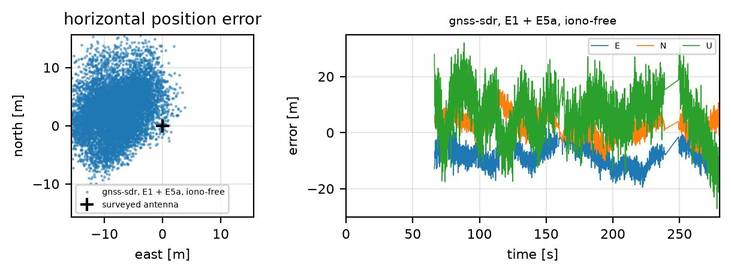
\includegraphics[width=1.0\linewidth]{gnss_sdr/x310_20261023T190000Z/galileo_pvt.jpg}
  \caption{PVT: position error of GNSS-SDR's own RTKLIB solution with respect to the surveyed antenna position.}
\end{figure}

\begin{table}[H]
  \centering
  \footnotesize
  \resizebox{\ifdim\width>\linewidth\linewidth\else\width\fi}{!}{%
  \begin{tabular}{l>{\centering\arraybackslash}p{4.2cm}}
    \hline
    \textbf{Solution} & \textbf{gnss-sdr, E1 + E5a, iono-free} \\
    \hline
    Solutions & 9278 \\
    Run with fix [\%] & 73 \\
    Mean E / N / U [m] & -8.1 / 2.7 / 6.0 \\
    Std E / N / U [m] & 3.8 / 4.0 / 8.4 \\
    RMS 2-D [m] & 10.2 \\
    RMS 3-D [m] & 14.5 \\
    95\% horiz. [m] & 15.0 \\
    \hline
  \end{tabular}}
  \caption{PVT: position error statistics with respect to the surveyed antenna (mean = accuracy, std = precision; \% of the run's seconds with a position; GNSS-SDR outputs several solutions per second).}
\end{table}




\subsection{Second record}
\begin{table}[H]
  \centering
  \begin{tabular}{|l|l|l|}
    \hline
    \textbf{Parameter} & \textbf{Channel 0} & \textbf{Channel 1} \\
    \hline
    Start time & \multicolumn{2}{>{\centering\arraybackslash}p{7cm}|}{2026-10-23 19:33:16 UTC} \\
    \hline
    Frequency & 1575.420 MHz (L1) & 1227.600 MHz (L2) \\
    \hline
    Duration & 300.0 s & 300.0 s \\
    \hline
    Sample rate & 4.000 MS/s & 4.000 MS/s \\
    \hline
    Sample type & \multicolumn{2}{>{\centering\arraybackslash}p{7cm}|}{signed complex 16-bit samples (I+Q), little-endian, as received from the X310 (sc16)} \\
    \hline
    Gain & 25.0 dB & 25.0 dB \\
    \hline
    Antenna & RX1 & RX2 \\
    \hline
    File size & 4800.0 MB & 4800.0 MB \\
    \hline
    Samples written & 1,200,000,000 & 1,200,000,000 \\
    \hline
    Lost samples & 0 & 0 \\
    \hline
    Clock source & \multicolumn{2}{>{\centering\arraybackslash}p{7cm}|}{external} \\
    \hline
    Time source & \multicolumn{2}{>{\centering\arraybackslash}p{7cm}|}{internal} \\
    \hline
    Motherboard & \multicolumn{2}{>{\centering\arraybackslash}p{7cm}|}{USRP X310} \\
    \hline
    Daughterboard & TwinRX RX0 & TwinRX RX1 \\
    \hline
    Recorder & \multicolumn{2}{>{\centering\arraybackslash}p{7cm}|}{UHD Python API} \\
    \hline
    GNSS-SDR configuration & \multicolumn{2}{>{\centering\arraybackslash}p{7cm}|}{\texttt{l1ca16bits4msps\_l2c16bits4msps.conf}} \\
    \hline
  \end{tabular}
  \caption{Metadata for recording \texttt{x310\_20261023T193310Z}, captured starting 2026-10-23T19:33:16.661684Z.}
\end{table}

\subsubsection{Signal source}
Raw I/Q samples of each channel analysed within the window [10, 10.5]~s after the start recording instant.

\begin{figure}[H]
  \centering
  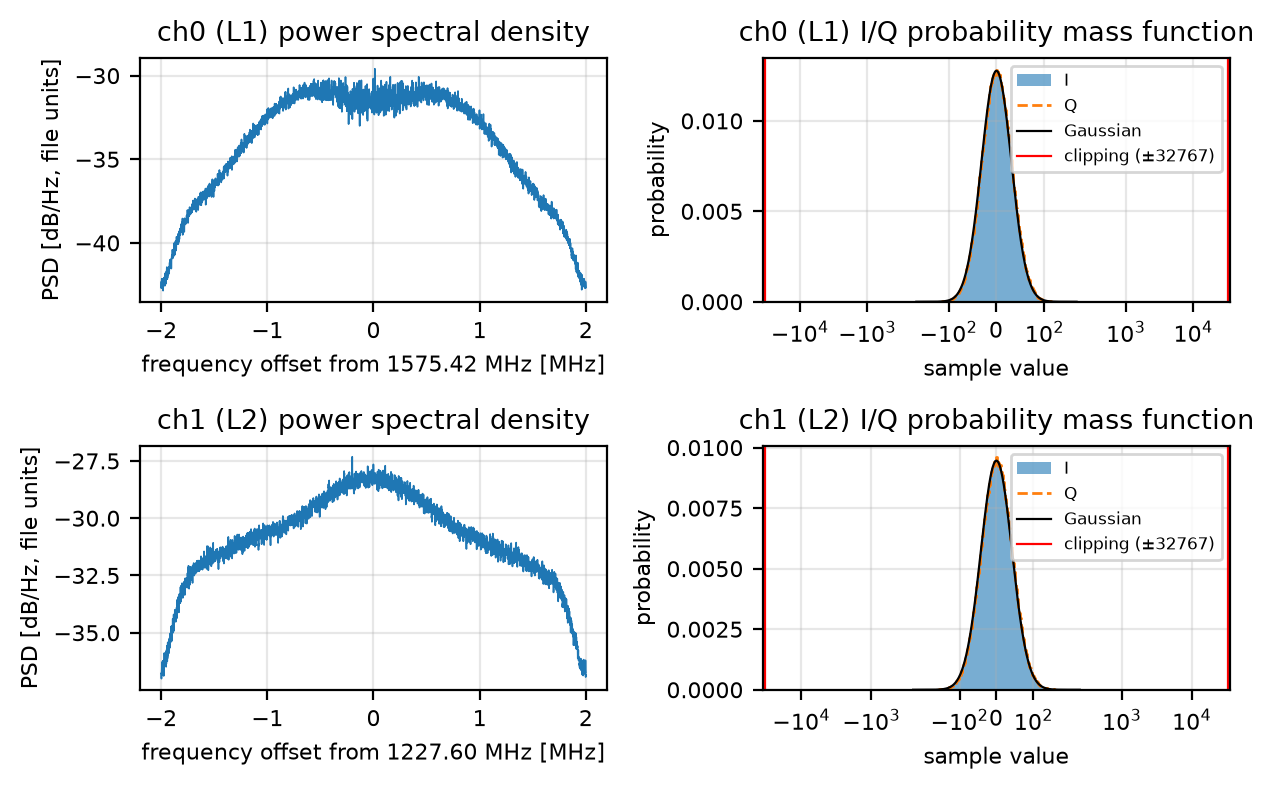
\includegraphics[width=1.0\linewidth]{gnss_sdr/x310_20261023T193310Z/source.png}
  \caption{Signal source: power spectral density (the receiver passband over a flat thermal-noise floor; GNSS signals are below the noise, so only interference would stand out) and probability mass functions of the integer I/Q sample values (Gaussian noise, centred, not clipped).}
\end{figure}

\begin{table}[H]
  \centering
  \footnotesize
  \resizebox{\ifdim\width>\linewidth\linewidth\else\width\fi}{!}{%
  \begin{tabular}{l>{\centering\arraybackslash}p{4.2cm}>{\centering\arraybackslash}p{4.2cm}}
    \hline
    \textbf{Channel} & \textbf{ch0} & \textbf{ch1} \\
    \hline
    Frequency [MHz] & 1575.42 & 1227.60 \\
    Rate [MS/s] & 4 & 4 \\
    Format & ci16\_le & ci16\_le \\
    Bytes per complex sample & 4 (2 for I, 2 for Q) & 4 (2 for I, 2 for Q) \\
    Full scale & $\pm$32767 & $\pm$32767 \\
    Gain [dB] & 25 & 25 \\
    Std I / Q & 31.2 / 31.2 & 42.1 / 42.2 \\
    Mean I / Q & -0.04 / 0.06 & 0.03 / -0.02 \\
    Min / max I & -164 / 155 & -205 / 216 \\
    Min / max Q & -155 / 165 & -203 / 212 \\
    Headroom\footnotemark & 1048.7 & 777.0 \\
    Clipped [\%] & 0.000 & 0.000 \\
    Lost samples & 0 & 0 \\
    \hline
  \end{tabular}}
  \caption{Signal source: sample statistics per channel (headroom: how many standard deviations of the noise fit before clipping).}
\end{table}

\footnotetext{Headroom $= A/\sigma$, where $A$ is the full scale of the sample format (127 for 8-bit, 32767 for 16-bit) and $\sigma$ the standard deviation of the I and Q samples together (both in file units, over the analysed window). For Gaussian noise, the fraction of clipped values is $2Q(A/\sigma)$, with $Q$ the Gaussian tail function: e.g. 0.003\,\% at $4.2\sigma$.}

\subsubsection{Signal conditioner}


\begin{table}[H]
  \centering
  \footnotesize
  \resizebox{\ifdim\width>\linewidth\linewidth\else\width\fi}{!}{%
  \begin{tabular}{l>{\centering\arraybackslash}p{4.2cm}>{\centering\arraybackslash}p{4.2cm}}
    \hline
    \textbf{Channel} & \textbf{ch0 (L1 C/A, E1)} & \textbf{ch1 (L2C)} \\
    \hline
    File format & ci16\_le & ci16\_le \\
    Source item type & ishort & ishort \\
    Data type adapter & Ishort\_To\_Complex & Ishort\_To\_Complex \\
    Input filter & Pass\_Through & Pass\_Through \\
    Resampling & Pass\_Through & Pass\_Through \\
    Rate [MS/s] & 4 $\to$ 4 & 4 $\to$ 4 \\
    \hline
  \end{tabular}}
  \caption{Signal conditioner: recorded format and rate to gnss-sdr's internal \texttt{gr\_complex} stream; both bands are read in lockstep by one \texttt{Multichannel\_File\_Signal\_Source}.}
\end{table}

\subsubsection{Acquisition}
Two-dimensional search over code delay and Doppler (one channel per band dumped; the others behave alike).

\begin{figure}[H]
  \centering
  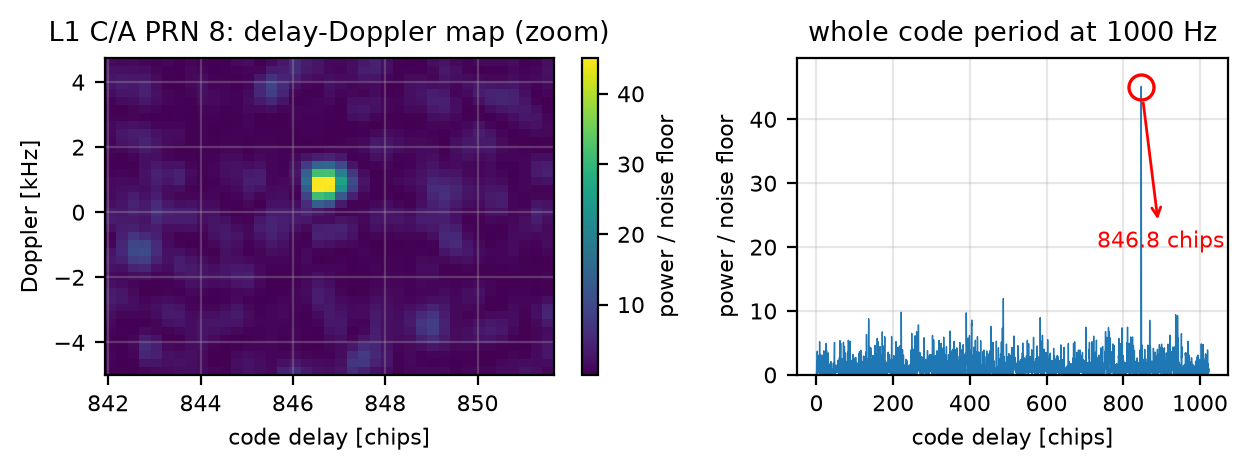
\includegraphics[width=1.0\linewidth]{gnss_sdr/x310_20261023T193310Z/acq_1C.png}
  \caption{Acquisition, L1 C/A: delay--Doppler search of PRN 8; one sharp peak (test statistic 62 vs threshold 44) at 1000~Hz and 846.8~chips.}
\end{figure}

\begin{figure}[H]
  \centering
  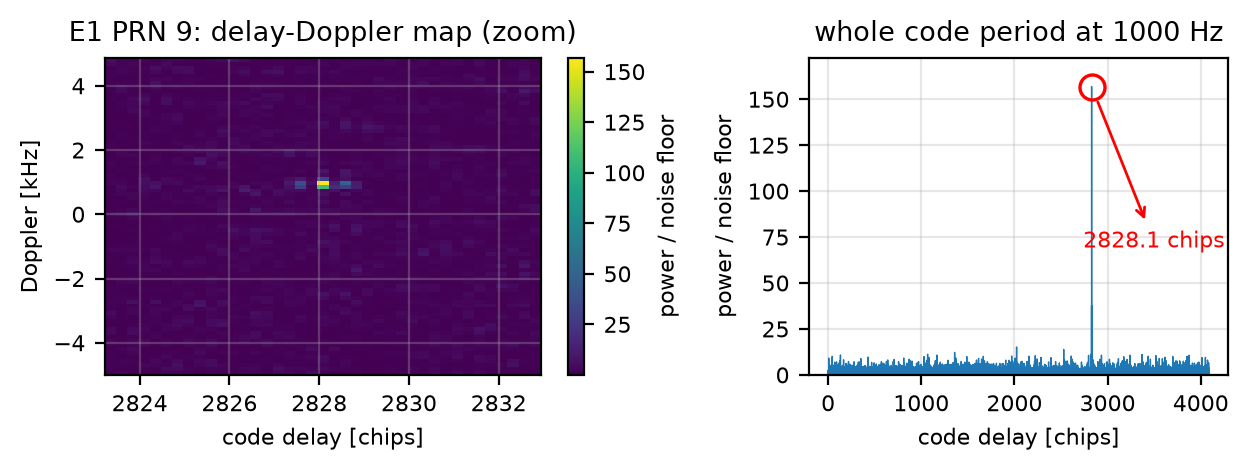
\includegraphics[width=1.0\linewidth]{gnss_sdr/x310_20261023T193310Z/acq_1B.png}
  \caption{Acquisition, E1: delay--Doppler search of PRN 9; one sharp peak (test statistic 211 vs threshold 48) at 1000~Hz and 2828.1~chips.}
\end{figure}

\begin{table}[H]
  \centering
  \footnotesize
  \resizebox{\ifdim\width>\linewidth\linewidth\else\width\fi}{!}{%
  \begin{tabular}{lrrrr}
    \hline
    \textbf{Band} & \textbf{Attempts} & \textbf{Detections} & \textbf{Detected PRNs} & \textbf{Best statistic / threshold\footnotemark} \\
    \hline
    L1 C/A & 7 & 1 & 8 & 1.4 \\
    L2C & \multicolumn{4}{l}{not dumped (search grid too large); acquired satellites: see the tracking table} \\
    E1 & 1 & 1 & 9 & 4.4 \\
    \hline
  \end{tabular}}
  \caption{Acquisition: search attempts of the dumped channel. Attempts on satellites that are not in view (or do not broadcast that signal, e.g. older GPS satellites on L5/L2C) are rejected below the threshold.}
\end{table}

\footnotetext{Margin of the band's strongest detection: the largest acquisition test statistic among the detected attempts (the correlation peak of the delay--Doppler grid, normalised by the power of the input samples searched, i.e. the noise power, since GNSS signals are below the noise) divided by the detection threshold, which GNSS-SDR derives from the configured probability of false alarm. A value of 1 is right at the detection limit; e.g. 2.5 means the peak cleared the threshold 2.5 times over.}

\subsubsection{Tracking}


\begin{figure}[H]
  \centering
  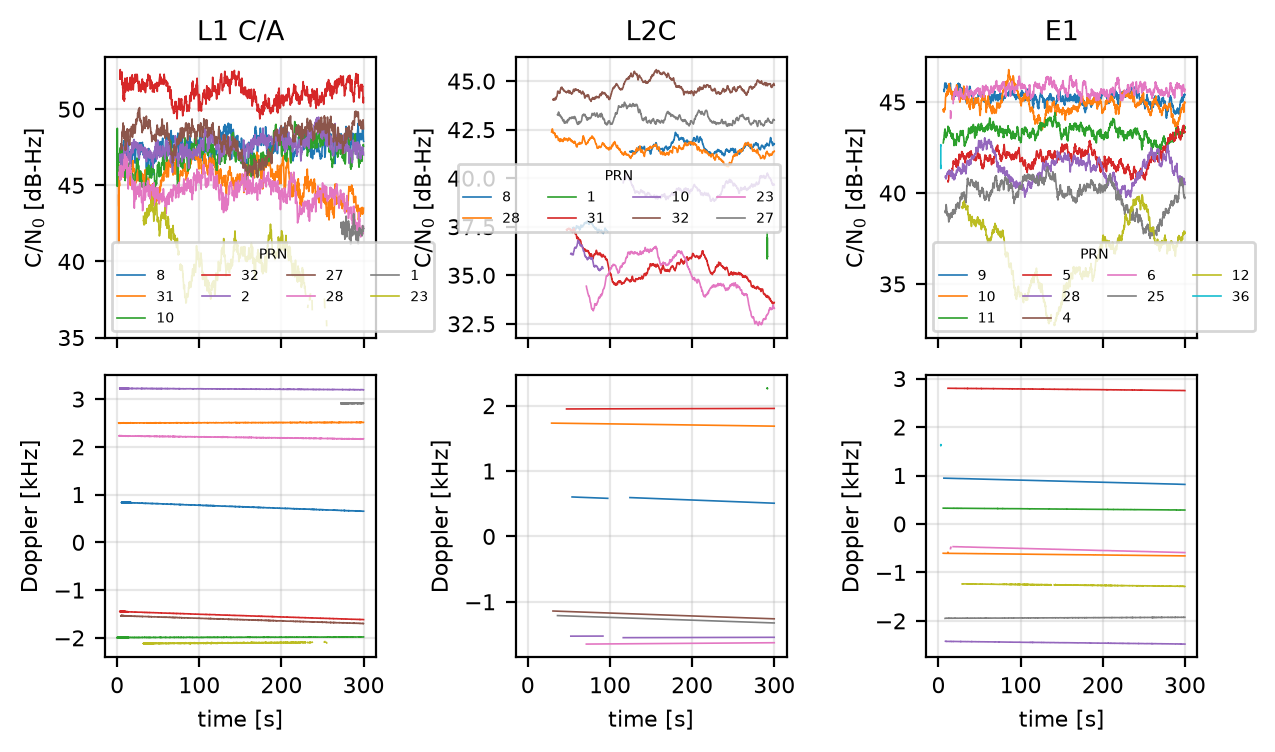
\includegraphics[width=1.0\linewidth]{gnss_sdr/x310_20261023T193310Z/tracking.png}
  \caption{Tracking: carrier-to-noise density ratio and carrier Doppler per satellite, while phase-locked (smooth Doppler curves = loops following the real satellite motion).}
\end{figure}

\begin{figure}[H]
  \centering
  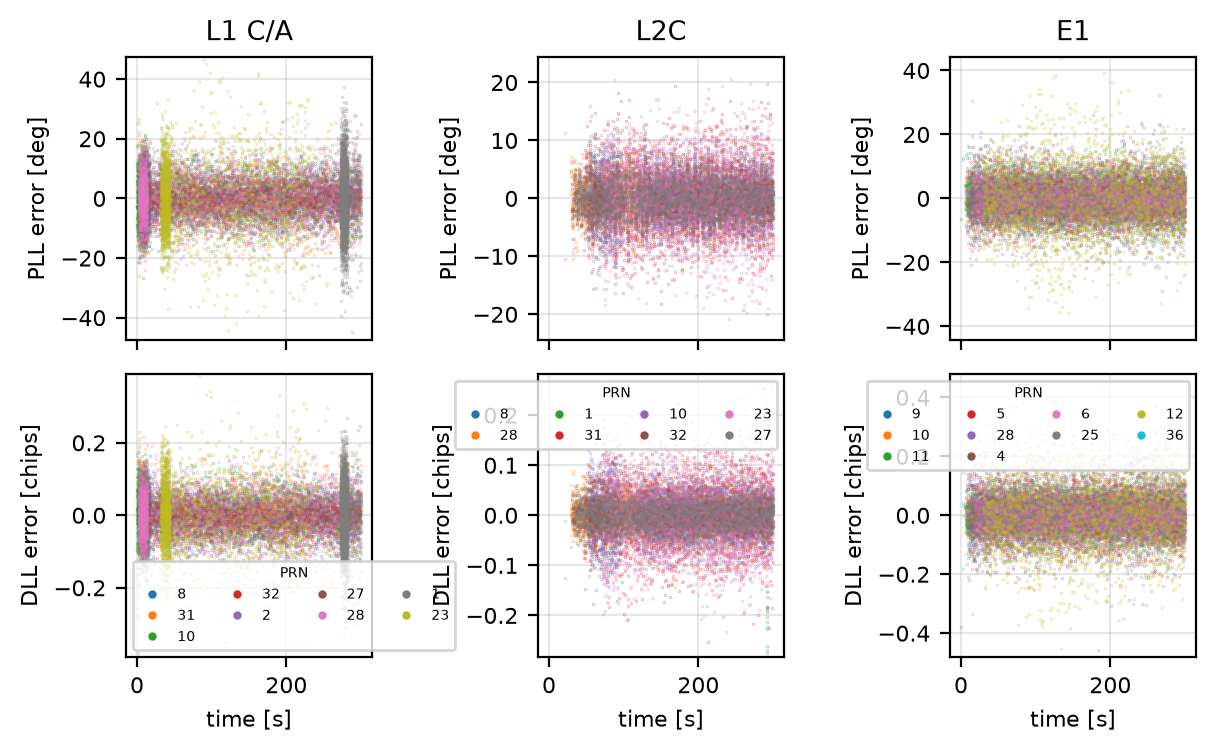
\includegraphics[width=1.0\linewidth]{gnss_sdr/x310_20261023T193310Z/tracking_errors.png}
  \caption{Tracking: loop errors per satellite while phase-locked, i.e. the discriminator outputs that the loops drive to zero: PLL carrier-phase error (degrees) and DLL code-delay error (chips) of every correlation. Noise centred on zero = clean tracking; its spread grows as C/N$_0$ drops, and jumps would mark cycle slips or a loop losing lock.}
\end{figure}

\begin{figure}[H]
  \centering
  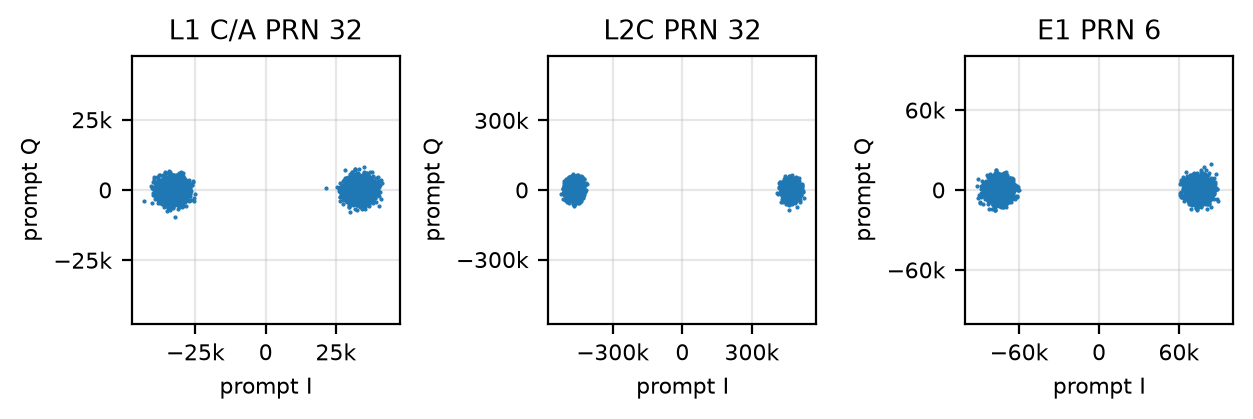
\includegraphics[width=1.0\linewidth]{gnss_sdr/x310_20261023T193310Z/tracking_iq.png}
  \caption{Tracking: prompt correlator outputs of the strongest satellite per band. Two tight clusters on one axis (the $\pm1$ data bits; GNSS-SDR's L5 tracking puts the data component on the Q axis), or, for the dataless pilots tracked for Galileo (E1-C, E5a-Q), the $\pm1$ chips of their secondary code, mean the PLL is phase-locked; a ring would mean it is not. \texttt{Prompt\_I}/\texttt{Prompt\_Q} are 32-bit floats (sums of the samples over one integration period, in file units): they never clip, only overflowing beyond $\pm 3.4\times10^{38}$, far above the $N\cdot\text{full scale}\cdot\sqrt{2}$ a sum of $N$ samples can reach.}
\end{figure}

\begin{table}[H]
  \centering
  \footnotesize
  \resizebox{\ifdim\width>\linewidth\linewidth\else\width\fi}{!}{%
  \begin{tabular}{lrrrrrrrr}
    \hline
    \textbf{Band} & \textbf{Ch.} & \textbf{PRN} & \textbf{Median C/N$_0$ [dB-Hz]} & \textbf{Phase-locked [\%]} & \textbf{Losses of lock} & \textbf{Tracked [s]} & \textbf{PLL error std [deg]} & \textbf{DLL error std [chips]} \\
    \hline
    L1 C/A & 0 & 8 & 47.3 & 91 & 0 & 297 & 6.1 & 0.049 \\
    L1 C/A & 1 & 31 & 45.8 & 100 & 0 & 298 & 7.6 & 0.061 \\
    L1 C/A & 2 & 10 & 46.7 & 100 & 0 & 300 & 6.7 & 0.053 \\
    L1 C/A & 3 & 32 & 51.5 & 94 & 0 & 298 & 3.9 & 0.030 \\
    L1 C/A & 4 & 2 & 47.3 & 95 & 0 & 298 & 6.1 & 0.047 \\
    L1 C/A & 5 & 27 & 48.2 & 88 & 0 & 299 & 5.7 & 0.043 \\
    L1 C/A & 6 & 28 & 45.3 & 96 & 0 & 299 & 8.1 & 0.061 \\
    L1 C/A & 7 & 1 & 42.2 & 79 & 1 & 30 & 11.1 & 0.085 \\
    L1 C/A & 7 & 23 & 42.7 & 83 & 1 & 232 & 12.3 & 0.095 \\
    L2C & 8 & 8 & 41.4 & 80 & 1 & 274 & 3.5 & 0.035 \\
    L2C & 9 & 28 & 41.5 & 97 & 0 & 279 & 3.3 & 0.031 \\
    L2C & 10 & 1 & 36.7 & 9 & 0 & 9 & 52.8 & 0.059 \\
    L2C & 11 & 31 & 35.4 & 91 & 0 & 280 & 5.9 & 0.065 \\
    L2C & 12 & 10 & 39.3 & 80 & 1 & 280 & 4.4 & 0.045 \\
    L2C & 13 & 32 & 44.6 & 97 & 0 & 279 & 2.7 & 0.022 \\
    L2C & 14 & 23 & 34.8 & 92 & 0 & 249 & 6.1 & 0.070 \\
    L2C & 15 & 27 & 43.1 & 95 & 0 & 279 & 2.9 & 0.026 \\
    E1 & 16 & 9 & 45.2 & 98 & 0 & 300 & 3.7 & 0.043 \\
    E1 & 17 & 10 & 44.9 & 98 & 0 & 300 & 4.3 & 0.048 \\
    E1 & 18 & 11 & 43.3 & 98 & 0 & 300 & 5.4 & 0.055 \\
    E1 & 19 & 5 & 41.9 & 97 & 0 & 297 & 5.8 & 0.068 \\
    E1 & 20 & 28 & 41.3 & 98 & 0 & 298 & 6.0 & 0.070 \\
    E1 & 21 & 4 & 26.4 & 1 & 1 & 11 & -- & -- \\
    E1 & 21 & 6 & 45.7 & 99 & 1 & 286 & 4.5 & 0.042 \\
    E1 & 22 & 25 & 40.0 & 98 & 0 & 298 & 7.5 & 0.086 \\
    E1 & 23 & 12 & 37.1 & 97 & 1 & 276 & 11.2 & 0.125 \\
    E1 & 23 & 36 & 44.3 & 0 & 1 & 21 & 48.0 & 0.107 \\
    \hline
  \end{tabular}}
  \caption{Tracking: per channel and satellite (phase-locked: carrier lock test $> 0.8$; loop error standard deviations while phase-locked).}
\end{table}

\subsubsection{Telemetry decoder}


\begin{figure}[H]
  \centering
  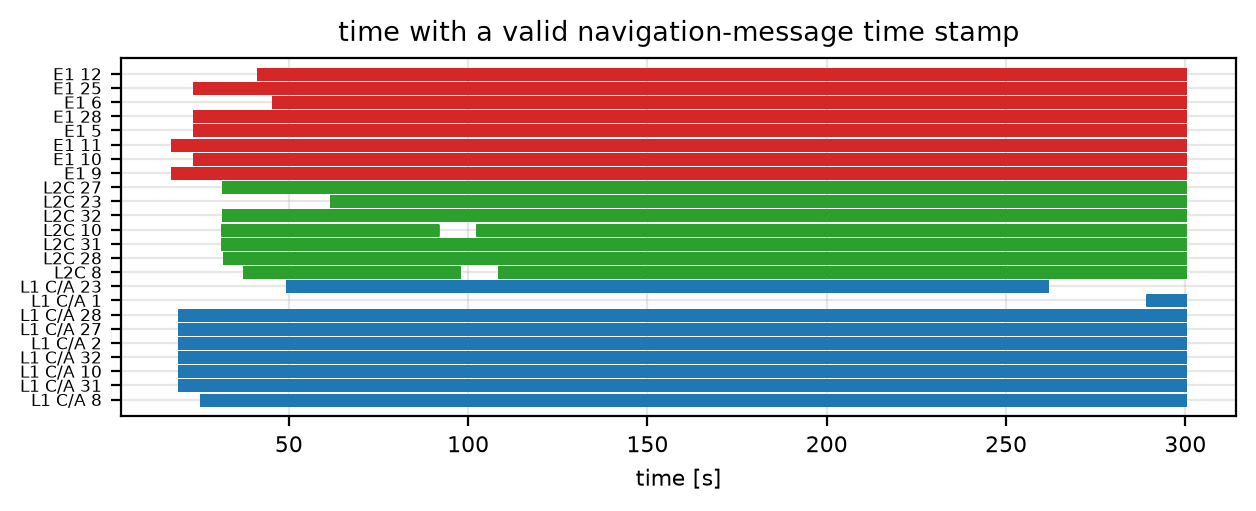
\includegraphics[width=1.0\linewidth]{gnss_sdr/x310_20261023T193310Z/telemetry.png}
  \caption{Telemetry decoder: per band and satellite, when the decoder delivered a valid transmit time (the first one comes after the first complete frame/message).}
\end{figure}

\begin{table}[H]
  \centering
  \footnotesize
  \resizebox{\ifdim\width>\linewidth\linewidth\else\width\fi}{!}{%
  \begin{tabular}{lrrrrr}
    \hline
    \textbf{Band} & \textbf{PRN} & \textbf{Messages decoded} & \textbf{Ephemeris} & \textbf{First valid at [s]} & \textbf{TOW [s]} \\
    \hline
    E1 & 5 & 27 & yes & 23.5 & 502438.0 \\
    E1 & 6 & 23 & yes & 45.5 & 502460.0 \\
    E1 & 9 & 26 & yes & 17.5 & 502432.0 \\
    E1 & 10 & 27 & yes & 23.5 & 502438.0 \\
    E1 & 11 & 27 & yes & 17.5 & 502432.0 \\
    E1 & 12 & 24 & yes & 41.5 & 502456.0 \\
    E1 & 25 & 27 & yes & 23.5 & 502438.0 \\
    E1 & 28 & 27 & yes & 23.5 & 502438.0 \\
    L1 C/A & 1 & 2 & no & 289.4 & 502704.0 \\
    L1 C/A & 2 & 46 & yes & 19.4 & 502434.0 \\
    L1 C/A & 8 & 45 & yes & 25.4 & 502440.0 \\
    L1 C/A & 10 & 45 & yes & 19.4 & 502434.0 \\
    L1 C/A & 23 & 36 & yes & 49.4 & 502464.0 \\
    L1 C/A & 27 & 43 & yes & 19.4 & 502434.0 \\
    L1 C/A & 28 & 45 & yes & 19.4 & 502434.0 \\
    L1 C/A & 31 & 47 & yes & 19.4 & 502434.0 \\
    L1 C/A & 32 & 45 & yes & 19.4 & 502434.0 \\
    L2C & 8 & 8 & yes & 37.4 & 0.0 \\
    L2C & 10 & 8 & yes & 31.5 & 0.0 \\
    L2C & 23 & 13 & yes & 61.6 & 0.0 \\
    L2C & 27 & 12 & yes & 31.6 & 0.0 \\
    L2C & 28 & 16 & yes & 31.8 & 0.0 \\
    L2C & 31 & 12 & yes & 31.4 & 0.0 \\
    L2C & 32 & 12 & yes & 31.5 & 0.0 \\
    \hline
  \end{tabular}}
  \caption{Telemetry decoder: L1 C/A LNAV subframes, L2C CNAV messages, E1 I/NAV words decoded, ephemeris obtained, and the first valid time of week.}
\end{table}

\subsubsection{Observables}
Pseudorange, carrier phase and Doppler of every channel at common receiver epochs.

\begin{figure}[H]
  \centering
  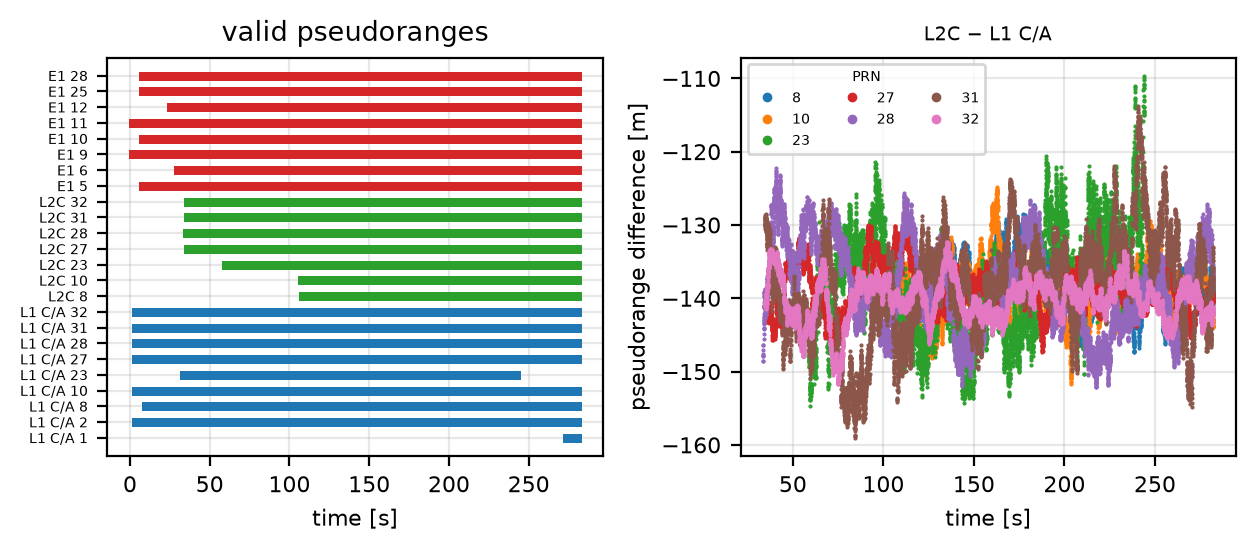
\includegraphics[width=1.0\linewidth]{gnss_sdr/x310_20261023T193310Z/observables.png}
  \caption{Observables: epochs with a valid pseudorange per band and satellite, and the difference between the two bands' pseudoranges of the same satellite (a constant receiver inter-band bias, the same for every satellite, plus the slowly varying ionospheric delay).}
\end{figure}

\begin{table}[H]
  \centering
  \footnotesize
  \resizebox{\ifdim\width>\linewidth\linewidth\else\width\fi}{!}{%
  \begin{tabular}{lrrrrrr}
    \hline
    \textbf{Difference} & \textbf{PRN} & \textbf{Common epochs} & \textbf{of run [\%]} & \textbf{Mean [m]} & \textbf{Std [m]} & \textbf{Drift [m/s]} \\
    \hline
    L2C $-$ L1 C/A & 8 & 8789 & 59 & -137.54 & 3.60 & -0.0130 \\
    L2C $-$ L1 C/A & 10 & 8829 & 59 & -138.91 & 3.87 & 0.0045 \\
    L2C $-$ L1 C/A & 23 & 9286 & 62 & -138.17 & 6.94 & 0.0399 \\
    L2C $-$ L1 C/A & 27 & 12381 & 83 & -138.90 & 3.03 & -0.0087 \\
    L2C $-$ L1 C/A & 28 & 12437 & 83 & -138.47 & 5.77 & -0.0274 \\
    L2C $-$ L1 C/A & 31 & 12393 & 83 & -138.52 & 7.00 & 0.0405 \\
    L2C $-$ L1 C/A & 32 & 12387 & 83 & -140.16 & 2.89 & 0.0019 \\
    \hline
  \end{tabular}}
  \caption{Observables: pseudorange difference between the two bands of each satellite at common epochs (similar means = shared receiver bias; std = code noise of both bands).}
\end{table}

\subsubsection{PVT}
Position from the pseudoranges and the decoded ephemeris, compared with the surveyed antenna position (-23.209433$^\circ$, -45.874875$^\circ$, 596.42~m).

\begin{figure}[H]
  \centering
  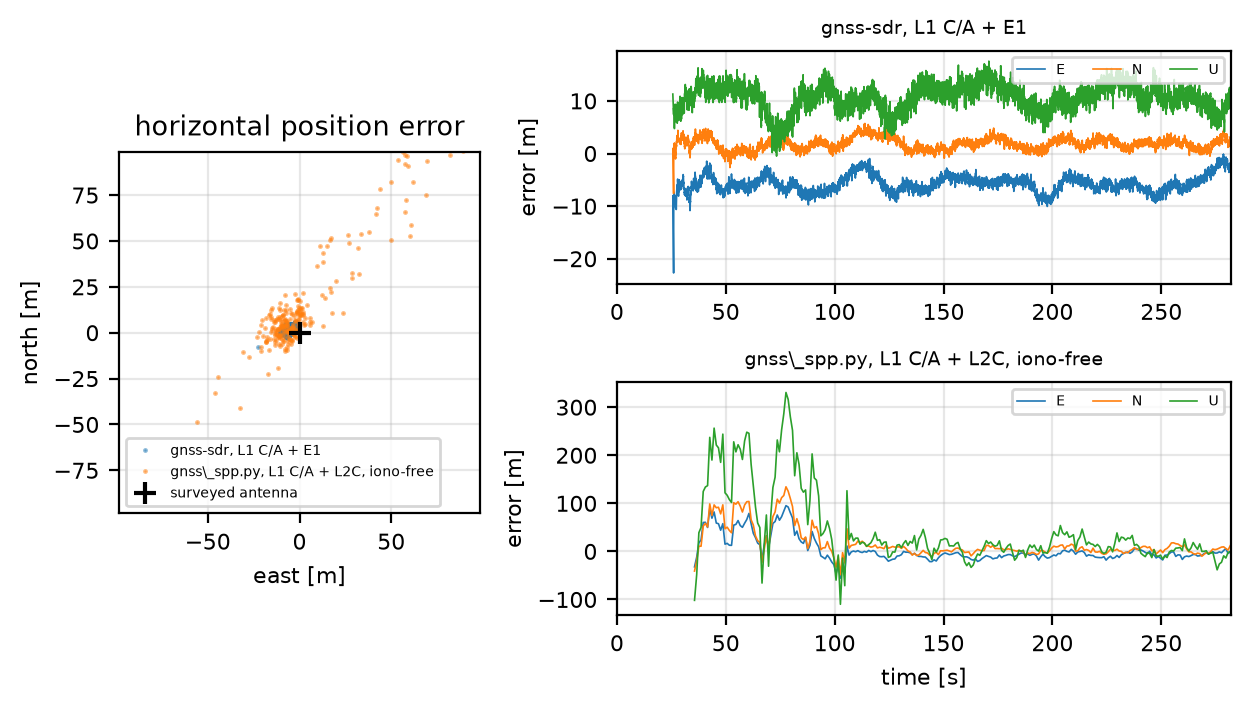
\includegraphics[width=1.0\linewidth]{gnss_sdr/x310_20261023T193310Z/pvt.png}
  \caption{PVT: position error with respect to the surveyed antenna position. gnss-sdr: GNSS-SDR's own RTKLIB solution (single frequency, broadcast ionosphere model). gnss\_spp.py: computed from gnss-sdr's observables and decoded GPS ephemeris, removing the ionospheric delay with the second band (pseudoranges carrier-smoothed over 100~s).}
\end{figure}

\begin{figure}[H]
  \centering
  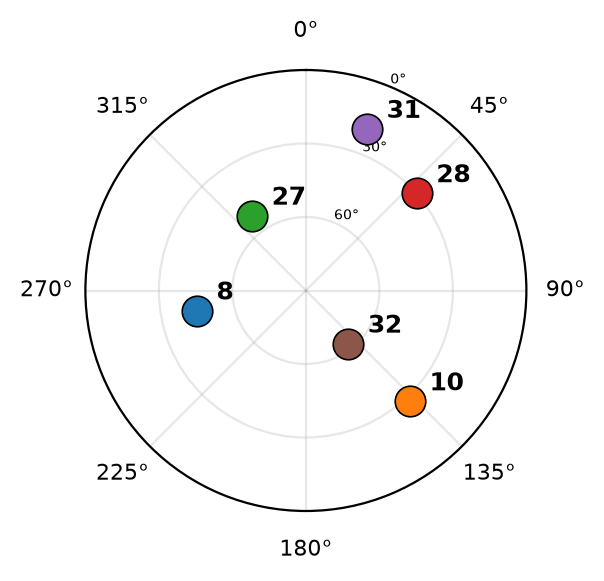
\includegraphics[width=0.45\linewidth]{gnss_sdr/x310_20261023T193310Z/skyplot.png}
  \caption{PVT: sky plot of the GPS satellites in the gnss\_spp.py dual-frequency solution (azimuth, elevation) during the recording.}
\end{figure}

\begin{table}[H]
  \centering
  \footnotesize
  \resizebox{\ifdim\width>\linewidth\linewidth\else\width\fi}{!}{%
  \begin{tabular}{l>{\centering\arraybackslash}p{4.2cm}>{\centering\arraybackslash}p{4.2cm}}
    \hline
    \textbf{Solution} & \textbf{gnss-sdr, L1 C/A + E1} & \textbf{gnss\_spp.py, L1 C/A + L2C, iono-free} \\
    \hline
    Solutions & 13328 & 247 \\
    Run with fix [\%] & 91 & 88 \\
    Mean E / N / U [m] & -5.8 / 1.8 / 10.6 & 3.3 / 16.8 / 42.9 \\
    Std E / N / U [m] & 1.6 / 1.2 / 2.5 & 26.5 / 32.0 / 78.1 \\
    RMS 2-D [m] & 6.4 & 44.9 \\
    RMS 3-D [m] & 12.6 & 99.8 \\
    95\% horiz. [m] & 8.4 & 116.1 \\
    \hline
  \end{tabular}}
  \caption{PVT: position error statistics with respect to the surveyed antenna (mean = accuracy, std = precision; \% of the run's seconds with a position; gnss-sdr outputs several solutions per second, gnss\_spp.py computes one per second).}
\end{table}




\section{Records on 24/10/2026}

\subsection{First record}
\begin{table}[H]
  \centering
  \begin{tabular}{|l|l|l|}
    \hline
    \textbf{Parameter} & \textbf{Channel 0} & \textbf{Channel 1} \\
    \hline
    Start time & \multicolumn{2}{>{\centering\arraybackslash}p{7cm}|}{2026-10-24 19:00:07 UTC} \\
    \hline
    Frequency & 1575.420 MHz (L1) & 1176.450 MHz (L5) \\
    \hline
    Duration & 300.0 s & 300.0 s \\
    \hline
    Sample rate & 4.000 MS/s & 20.000 MS/s \\
    \hline
    Sample type & \multicolumn{2}{>{\centering\arraybackslash}p{7cm}|}{signed complex 8-bit samples (I+Q), converted on the host from the X310's sc16} \\
    \hline
    Gain & 25.0 dB & 25.0 dB \\
    \hline
    Antenna & RX1 & RX2 \\
    \hline
    File size & 2400.0 MB & 12000.0 MB \\
    \hline
    Samples written & 1,200,000,000 & 6,000,000,000 \\
    \hline
    Lost samples & 0 & 2115024 \\
    \hline
    Clock source & \multicolumn{2}{>{\centering\arraybackslash}p{7cm}|}{external} \\
    \hline
    Time source & \multicolumn{2}{>{\centering\arraybackslash}p{7cm}|}{internal} \\
    \hline
    Motherboard & \multicolumn{2}{>{\centering\arraybackslash}p{7cm}|}{USRP X310} \\
    \hline
    Daughterboard & TwinRX RX0 & TwinRX RX1 \\
    \hline
    Recorder & \multicolumn{2}{>{\centering\arraybackslash}p{7cm}|}{UHD Python API} \\
    \hline
    GNSS-SDR configuration & \multicolumn{2}{>{\centering\arraybackslash}p{7cm}|}{\texttt{l1ca8bits4msps\_l5\_8bits20msps.conf}, \texttt{e1\_8bits4msps\_e5a\_8bits20msps.conf}} \\
    \hline
  \end{tabular}
  \caption{Metadata for recording \texttt{x310\_20261024T190000Z}, captured starting 2026-10-24T19:00:07.446070Z.}
\end{table}

\subsubsection{Signal source}
Raw I/Q samples of each channel analysed within the window [10, 10.5]~s after the start recording instant.

\begin{figure}[H]
  \centering
  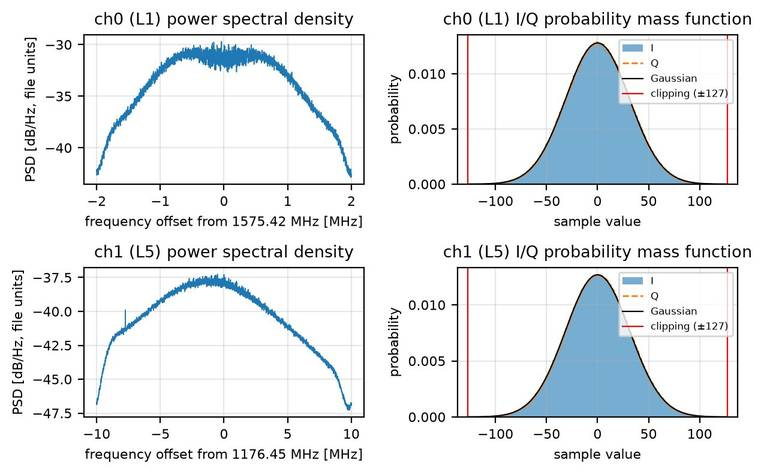
\includegraphics[width=1.0\linewidth]{gnss_sdr/x310_20261024T190000Z/source.jpg}
  \caption{Signal source: power spectral density (the receiver passband over a flat thermal-noise floor; GNSS signals are below the noise, so only interference would stand out) and probability mass functions of the integer I/Q sample values (Gaussian noise, centred, not clipped).}
\end{figure}

\begin{table}[H]
  \centering
  \footnotesize
  \resizebox{\ifdim\width>\linewidth\linewidth\else\width\fi}{!}{%
  \begin{tabular}{l>{\centering\arraybackslash}p{4.2cm}>{\centering\arraybackslash}p{4.2cm}}
    \hline
    \textbf{Channel} & \textbf{ch0} & \textbf{ch1} \\
    \hline
    Frequency [MHz] & 1575.42 & 1176.45 \\
    Rate [MS/s] & 4 & 20 \\
    Format & ci8 & ci8 \\
    Bytes per complex sample & 2 (1 for I, 1 for Q) & 2 (1 for I, 1 for Q) \\
    Full scale & $\pm$127 & $\pm$127 \\
    Gain [dB] & 25 & 25 \\
    Std I / Q & 31.2 / 31.2 & 31.4 / 31.4 \\
    Mean I / Q & -0.10 / -0.16 & -0.01 / -0.01 \\
    Min / max I & -127 / 127 & -127 / 127 \\
    Min / max Q & -127 / 127 & -127 / 127 \\
    Headroom\footnotemark & 4.1 & 4.0 \\
    Clipped [\%] & 0.004 & 0.005 \\
    Lost samples & 0 & 2,115,024 \\
    \hline
  \end{tabular}}
  \caption{Signal source: sample statistics per channel (headroom: how many standard deviations of the noise fit before clipping).}
\end{table}

\footnotetext{Headroom $= A/\sigma$, where $A$ is the full scale of the sample format (127 for 8-bit, 32767 for 16-bit) and $\sigma$ the standard deviation of the I and Q samples together (both in file units, over the analysed window). For Gaussian noise, the fraction of clipped values is $2Q(A/\sigma)$, with $Q$ the Gaussian tail function: e.g. 0.003\,\% at $4.2\sigma$.}

\subsubsection{Signal conditioner}


\begin{table}[H]
  \centering
  \footnotesize
  \resizebox{\ifdim\width>\linewidth\linewidth\else\width\fi}{!}{%
  \begin{tabular}{l>{\centering\arraybackslash}p{4.2cm}>{\centering\arraybackslash}p{4.2cm}}
    \hline
    \textbf{Channel} & \textbf{ch0 (L1 C/A)} & \textbf{ch1 (L5)} \\
    \hline
    File format & ci8 & ci8 \\
    Source item type & ibyte & ibyte \\
    Data type adapter & Ibyte\_To\_Complex & Ibyte\_To\_Complex \\
    Input filter & Pass\_Through & Pass\_Through \\
    Resampling & $\times$5 zero-order hold, offline (\texttt{upsample\_iq.py}) & Pass\_Through \\
    Rate [MS/s] & 4 $\to$ 20 & 20 $\to$ 20 \\
    \hline
  \end{tabular}}
  \caption{Signal conditioner: recorded format and rate to gnss-sdr's internal \texttt{gr\_complex} stream; both bands are read in lockstep by one \texttt{Multichannel\_File\_Signal\_Source}.}
\end{table}

\subsubsection{Acquisition}
Two-dimensional search over code delay and Doppler (one channel per band dumped; the others behave alike).

\begin{figure}[H]
  \centering
  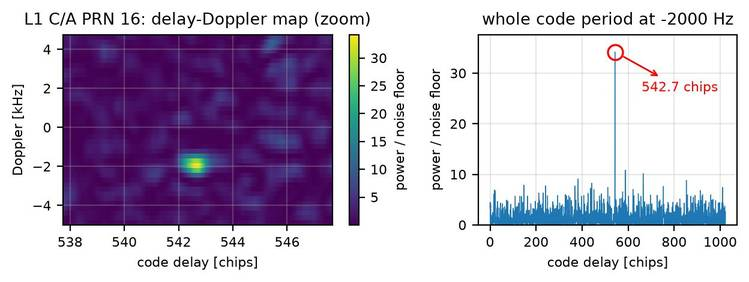
\includegraphics[width=1.0\linewidth]{gnss_sdr/x310_20261024T190000Z/acq_1C.jpg}
  \caption{Acquisition, L1 C/A: delay--Doppler search of PRN 16; one sharp peak (test statistic 49 vs threshold 47) at -2000~Hz and 542.7~chips.}
\end{figure}

\begin{table}[H]
  \centering
  \footnotesize
  \resizebox{\ifdim\width>\linewidth\linewidth\else\width\fi}{!}{%
  \begin{tabular}{lrrrr}
    \hline
    \textbf{Band} & \textbf{Attempts} & \textbf{Detections} & \textbf{Detected PRNs} & \textbf{Best statistic / threshold\footnotemark} \\
    \hline
    L1 C/A & 2 & 1 & 16 & 1.0 \\
    L5 & 2016 & 0 & -- & -- \\
    \hline
  \end{tabular}}
  \caption{Acquisition: search attempts of the dumped channel. Attempts on satellites that are not in view (or do not broadcast that signal, e.g. older GPS satellites on L5/L2C) are rejected below the threshold.}
\end{table}

\footnotetext{Margin of the band's strongest detection: the largest acquisition test statistic among the detected attempts (the correlation peak of the delay--Doppler grid, normalised by the power of the input samples searched, i.e. the noise power, since GNSS signals are below the noise) divided by the detection threshold, which GNSS-SDR derives from the configured probability of false alarm. A value of 1 is right at the detection limit; e.g. 2.5 means the peak cleared the threshold 2.5 times over.}

\subsubsection{Tracking}


\begin{figure}[H]
  \centering
  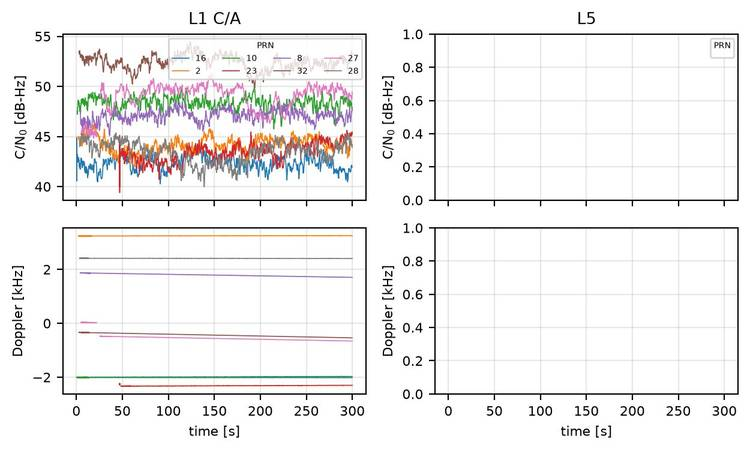
\includegraphics[width=1.0\linewidth]{gnss_sdr/x310_20261024T190000Z/tracking.jpg}
  \caption{Tracking: carrier-to-noise density ratio and carrier Doppler per satellite, while phase-locked (smooth Doppler curves = loops following the real satellite motion).}
\end{figure}

\begin{figure}[H]
  \centering
  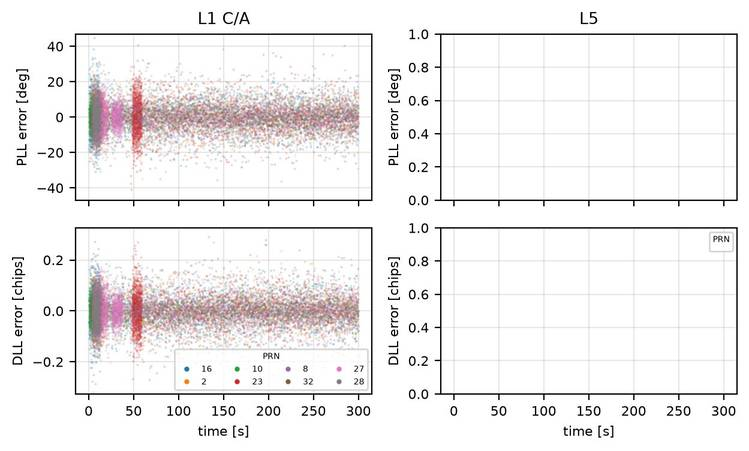
\includegraphics[width=1.0\linewidth]{gnss_sdr/x310_20261024T190000Z/tracking_errors.jpg}
  \caption{Tracking: loop errors per satellite while phase-locked, i.e. the discriminator outputs that the loops drive to zero: PLL carrier-phase error (degrees) and DLL code-delay error (chips) of every correlation. Noise centred on zero = clean tracking; its spread grows as C/N$_0$ drops, and jumps would mark cycle slips or a loop losing lock.}
\end{figure}

\begin{figure}[H]
  \centering
  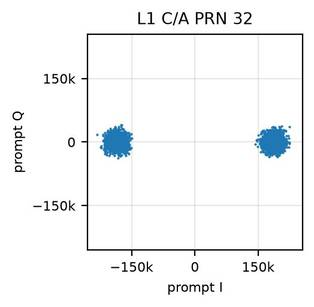
\includegraphics[width=1.0\linewidth]{gnss_sdr/x310_20261024T190000Z/tracking_iq.jpg}
  \caption{Tracking: prompt correlator outputs of the strongest satellite per band. Two tight clusters on one axis (the $\pm1$ data bits; GNSS-SDR's L5 tracking puts the data component on the Q axis), or, for the dataless pilots tracked for Galileo (E1-C, E5a-Q), the $\pm1$ chips of their secondary code, mean the PLL is phase-locked; a ring would mean it is not. \texttt{Prompt\_I}/\texttt{Prompt\_Q} are 32-bit floats (sums of the samples over one integration period, in file units): they never clip, only overflowing beyond $\pm 3.4\times10^{38}$, far above the $N\cdot\text{full scale}\cdot\sqrt{2}$ a sum of $N$ samples can reach.}
\end{figure}

\begin{table}[H]
  \centering
  \footnotesize
  \resizebox{\ifdim\width>\linewidth\linewidth\else\width\fi}{!}{%
  \begin{tabular}{lrrrrrrrr}
    \hline
    \textbf{Band} & \textbf{Ch.} & \textbf{PRN} & \textbf{Median C/N$_0$ [dB-Hz]} & \textbf{Phase-locked [\%]} & \textbf{Losses of lock} & \textbf{Tracked [s]} & \textbf{PLL error std [deg]} & \textbf{DLL error std [chips]} \\
    \hline
    L1 C/A & 0 & 16 & 42.3 & 100 & 0 & 300 & 11.1 & 0.079 \\
    L1 C/A & 1 & 2 & 44.7 & 97 & 0 & 299 & 8.4 & 0.061 \\
    L1 C/A & 2 & 10 & 48.4 & 98 & 0 & 300 & 5.5 & 0.039 \\
    L1 C/A & 3 & 23 & 43.3 & 95 & 0 & 253 & 11.1 & 0.072 \\
    L1 C/A & 4 & 8 & 46.8 & 92 & 0 & 298 & 6.6 & 0.050 \\
    L1 C/A & 5 & 32 & 52.7 & 94 & 0 & 299 & 3.5 & 0.024 \\
    L1 C/A & 6 & 27 & 47.4 & 88 & 1 & 296 & 6.2 & 0.046 \\
    L1 C/A & 7 & 28 & 44.2 & 90 & 0 & 299 & 9.3 & 0.067 \\
    \hline
  \end{tabular}}
  \caption{Tracking: per channel and satellite (phase-locked: carrier lock test $> 0.8$; loop error standard deviations while phase-locked).}
\end{table}

\subsubsection{Telemetry decoder}


\begin{figure}[H]
  \centering
  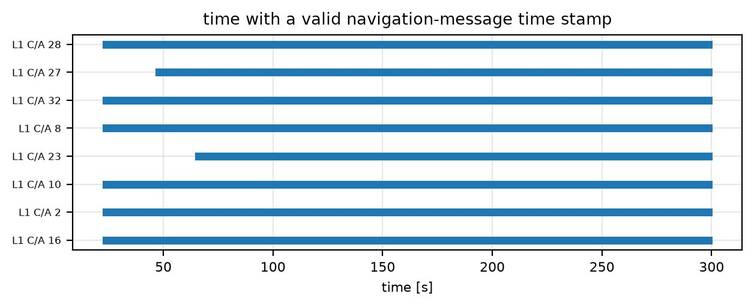
\includegraphics[width=1.0\linewidth]{gnss_sdr/x310_20261024T190000Z/telemetry.jpg}
  \caption{Telemetry decoder: per band and satellite, when the decoder delivered a valid transmit time (the first one comes after the first complete frame/message).}
\end{figure}

\begin{table}[H]
  \centering
  \footnotesize
  \resizebox{\ifdim\width>\linewidth\linewidth\else\width\fi}{!}{%
  \begin{tabular}{lrrrrr}
    \hline
    \textbf{Band} & \textbf{PRN} & \textbf{Messages decoded} & \textbf{Ephemeris} & \textbf{First valid at [s]} & \textbf{TOW [s]} \\
    \hline
    L1 C/A & 2 & 45 & yes & 22.6 & 586848.0 \\
    L1 C/A & 8 & 46 & yes & 22.6 & 586848.0 \\
    L1 C/A & 10 & 46 & yes & 22.6 & 586848.0 \\
    L1 C/A & 16 & 46 & yes & 22.6 & 586848.0 \\
    L1 C/A & 23 & 39 & yes & 64.6 & 586890.0 \\
    L1 C/A & 27 & 43 & yes & 46.6 & 586872.0 \\
    L1 C/A & 28 & 45 & yes & 22.6 & 586848.0 \\
    L1 C/A & 32 & 47 & yes & 22.6 & 586848.0 \\
    \hline
  \end{tabular}}
  \caption{Telemetry decoder: L1 C/A LNAV subframes, L5 CNAV messages decoded, ephemeris obtained, and the first valid time of week.}
\end{table}

\subsubsection{Observables}
Pseudorange, carrier phase and Doppler of every channel at common receiver epochs.

\begin{figure}[H]
  \centering
  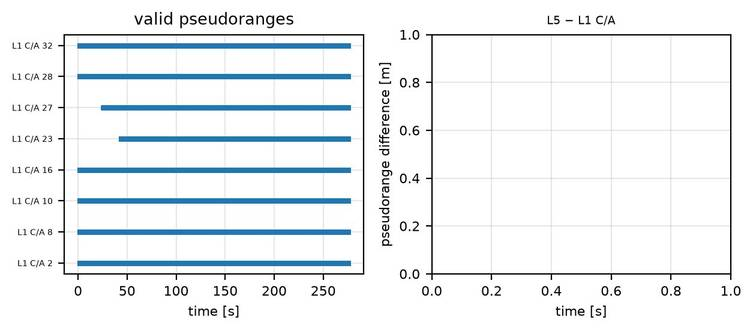
\includegraphics[width=1.0\linewidth]{gnss_sdr/x310_20261024T190000Z/observables.jpg}
  \caption{Observables: epochs with a valid pseudorange per band and satellite, and the difference between the two bands' pseudoranges of the same satellite (a constant receiver inter-band bias, the same for every satellite, plus the slowly varying ionospheric delay).}
\end{figure}

\textit{Not produced: epochs with pseudoranges on both bands (L5 $-$ L1 C/A).}

\subsubsection{PVT}
Position from the pseudoranges and the decoded ephemeris, compared with the surveyed antenna position (-23.209433$^\circ$, -45.874875$^\circ$, 596.42~m).

\begin{figure}[H]
  \centering
  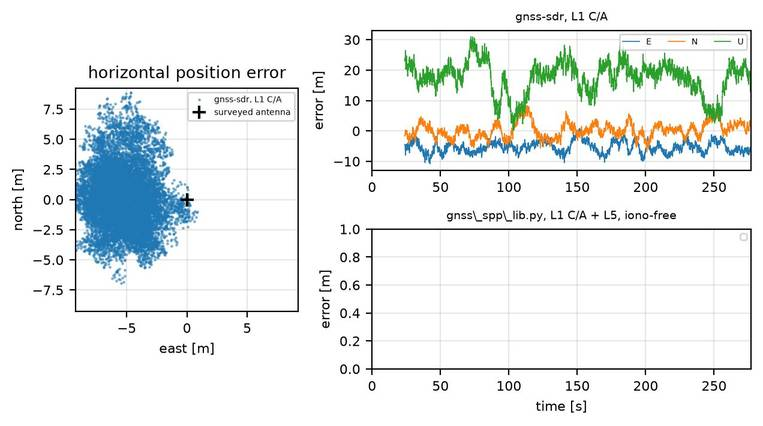
\includegraphics[width=1.0\linewidth]{gnss_sdr/x310_20261024T190000Z/pvt.jpg}
  \caption{PVT: position error of GNSS-SDR's own RTKLIB solution with respect to the surveyed antenna position (single frequency, broadcast ionosphere model).}
\end{figure}

\begin{table}[H]
  \centering
  \footnotesize
  \resizebox{\ifdim\width>\linewidth\linewidth\else\width\fi}{!}{%
  \begin{tabular}{l>{\centering\arraybackslash}p{4.2cm}}
    \hline
    \textbf{Solution} & \textbf{gnss-sdr, L1 C/A} \\
    \hline
    Solutions & 13160 \\
    Run with fix [\%] & 92 \\
    Mean E / N / U [m] & -5.3 / 0.3 / 17.5 \\
    Std E / N / U [m] & 1.9 / 2.5 / 5.4 \\
    RMS 2-D [m] & 6.2 \\
    RMS 3-D [m] & 19.3 \\
    95\% horiz. [m] & 8.7 \\
    \hline
  \end{tabular}}
  \caption{PVT: position error statistics with respect to the surveyed antenna (mean = accuracy, std = precision; \% of the run's seconds with a position; GNSS-SDR outputs several solutions per second).}
\end{table}


\subsubsection{Signal conditioner (Galileo E1 + E5a)}


\begin{table}[H]
  \centering
  \footnotesize
  \resizebox{\ifdim\width>\linewidth\linewidth\else\width\fi}{!}{%
  \begin{tabular}{l>{\centering\arraybackslash}p{4.2cm}>{\centering\arraybackslash}p{4.2cm}}
    \hline
    \textbf{Channel} & \textbf{ch0 (E1)} & \textbf{ch1 (E5a)} \\
    \hline
    File format & ci8 & ci8 \\
    Source item type & ibyte & ibyte \\
    Data type adapter & Ibyte\_To\_Complex & Ibyte\_To\_Complex \\
    Input filter & Pass\_Through & Pass\_Through \\
    Resampling & $\times$5 zero-order hold, offline (\texttt{upsample\_iq.py}) & Pass\_Through \\
    Rate [MS/s] & 4 $\to$ 20 & 20 $\to$ 20 \\
    \hline
  \end{tabular}}
  \caption{Signal conditioner: recorded format and rate to gnss-sdr's internal \texttt{gr\_complex} stream; both bands are read in lockstep by one \texttt{Multichannel\_File\_Signal\_Source}.}
\end{table}

\subsubsection{Acquisition (Galileo E1 + E5a)}
Two-dimensional search over code delay and Doppler (one channel per band dumped; the others behave alike).

\begin{figure}[H]
  \centering
  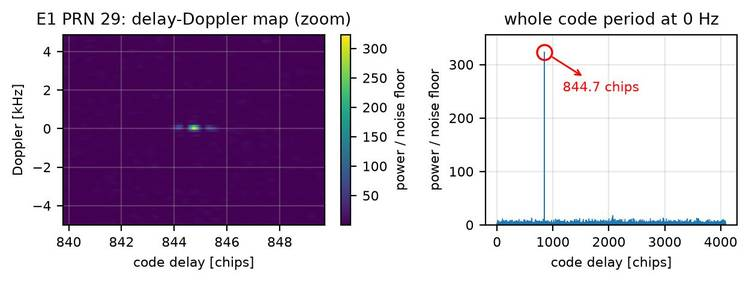
\includegraphics[width=1.0\linewidth]{gnss_sdr/x310_20261024T190000Z/galileo_acq_1B.jpg}
  \caption{Acquisition, E1: delay--Doppler search of PRN 29; one sharp peak (test statistic 450 vs threshold 52) at 0~Hz and 844.7~chips.}
\end{figure}

\begin{figure}[H]
  \centering
  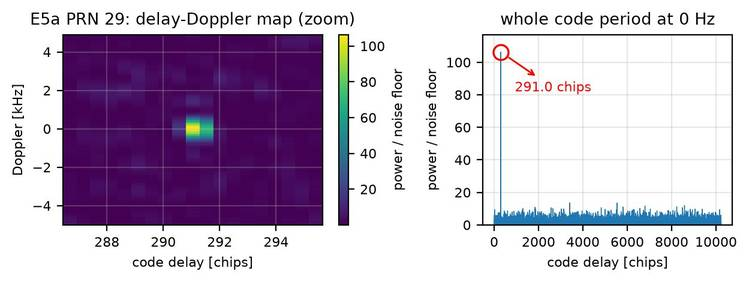
\includegraphics[width=1.0\linewidth]{gnss_sdr/x310_20261024T190000Z/galileo_acq_5X.jpg}
  \caption{Acquisition, E5a: delay--Doppler search of PRN 29; one sharp peak (test statistic 149 vs threshold 49) at 27~Hz and 291.0~chips.}
\end{figure}

\begin{table}[H]
  \centering
  \footnotesize
  \resizebox{\ifdim\width>\linewidth\linewidth\else\width\fi}{!}{%
  \begin{tabular}{lrrrr}
    \hline
    \textbf{Band} & \textbf{Attempts} & \textbf{Detections} & \textbf{Detected PRNs} & \textbf{Best statistic / threshold\footnotemark} \\
    \hline
    E1 & 4 & 1 & 29 & 8.7 \\
    E5a & 1 & 1 & 29 & 3.0 \\
    \hline
  \end{tabular}}
  \caption{Acquisition: search attempts of the dumped channel. Attempts on satellites that are not in view (or do not broadcast that signal, e.g. older GPS satellites on L5/L2C) are rejected below the threshold.}
\end{table}

\footnotetext{Margin of the band's strongest detection: the largest acquisition test statistic among the detected attempts (the correlation peak of the delay--Doppler grid, normalised by the power of the input samples searched, i.e. the noise power, since GNSS signals are below the noise) divided by the detection threshold, which GNSS-SDR derives from the configured probability of false alarm. A value of 1 is right at the detection limit; e.g. 2.5 means the peak cleared the threshold 2.5 times over.}

\subsubsection{Tracking (Galileo E1 + E5a)}


\begin{figure}[H]
  \centering
  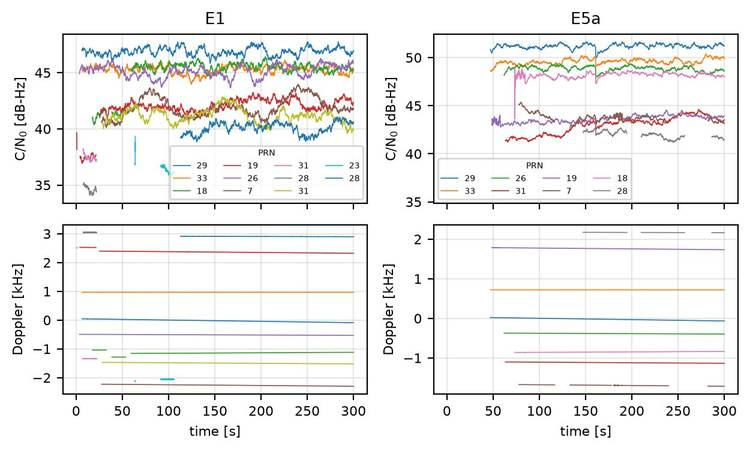
\includegraphics[width=1.0\linewidth]{gnss_sdr/x310_20261024T190000Z/galileo_tracking.jpg}
  \caption{Tracking: carrier-to-noise density ratio and carrier Doppler per satellite, while phase-locked (smooth Doppler curves = loops following the real satellite motion).}
\end{figure}

\begin{figure}[H]
  \centering
  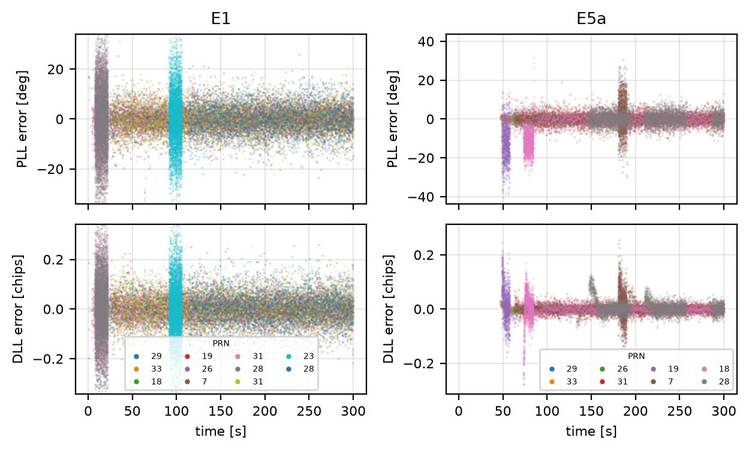
\includegraphics[width=1.0\linewidth]{gnss_sdr/x310_20261024T190000Z/galileo_tracking_errors.jpg}
  \caption{Tracking: loop errors per satellite while phase-locked, i.e. the discriminator outputs that the loops drive to zero: PLL carrier-phase error (degrees) and DLL code-delay error (chips) of every correlation. Noise centred on zero = clean tracking; its spread grows as C/N$_0$ drops, and jumps would mark cycle slips or a loop losing lock.}
\end{figure}

\begin{figure}[H]
  \centering
  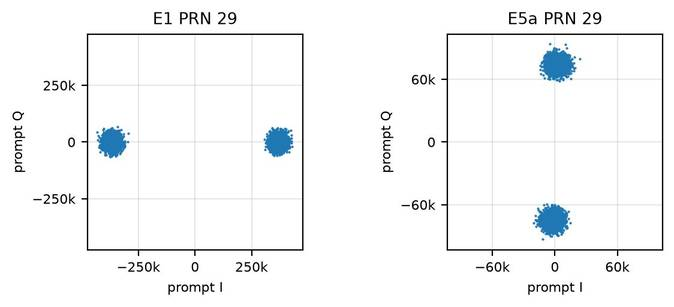
\includegraphics[width=1.0\linewidth]{gnss_sdr/x310_20261024T190000Z/galileo_tracking_iq.jpg}
  \caption{Tracking: prompt correlator outputs of the strongest satellite per band. Two tight clusters on one axis (the $\pm1$ data bits; GNSS-SDR's L5 tracking puts the data component on the Q axis), or, for the dataless pilots tracked for Galileo (E1-C, E5a-Q), the $\pm1$ chips of their secondary code, mean the PLL is phase-locked; a ring would mean it is not. \texttt{Prompt\_I}/\texttt{Prompt\_Q} are 32-bit floats (sums of the samples over one integration period, in file units): they never clip, only overflowing beyond $\pm 3.4\times10^{38}$, far above the $N\cdot\text{full scale}\cdot\sqrt{2}$ a sum of $N$ samples can reach.}
\end{figure}

\begin{table}[H]
  \centering
  \footnotesize
  \resizebox{\ifdim\width>\linewidth\linewidth\else\width\fi}{!}{%
  \begin{tabular}{lrrrrrrrr}
    \hline
    \textbf{Band} & \textbf{Ch.} & \textbf{PRN} & \textbf{Median C/N$_0$ [dB-Hz]} & \textbf{Phase-locked [\%]} & \textbf{Losses of lock} & \textbf{Tracked [s]} & \textbf{PLL error std [deg]} & \textbf{DLL error std [chips]} \\
    \hline
    E1 & 0 & 29 & 46.9 & 98 & 0 & 299 & 3.5 & 0.036 \\
    E1 & 1 & 33 & 45.3 & 98 & 0 & 299 & 3.7 & 0.038 \\
    E1 & 2 & 18 & 45.4 & 91 & 3 & 299 & 4.4 & 0.046 \\
    E1 & 3 & 19 & 42.0 & 98 & 1 & 299 & 6.3 & 0.065 \\
    E1 & 4 & 26 & 45.2 & 99 & 0 & 299 & 4.1 & 0.043 \\
    E1 & 5 & 7 & 41.8 & 98 & 1 & 277 & 5.7 & 0.061 \\
    E1 & 5 & 31 & 37.5 & 71 & 1 & 21 & 10.3 & 0.105 \\
    E1 & 6 & 28 & 34.9 & 68 & 1 & 21 & 14.2 & 0.139 \\
    E1 & 6 & 31 & 41.1 & 98 & 1 & 276 & 6.5 & 0.070 \\
    E1 & 7 & 23 & 39.8 & 14 & 5 & 105 & 12.1 & 0.116 \\
    E1 & 7 & 28 & 40.1 & 97 & 5 & 193 & 7.0 & 0.076 \\
    E5a & 8 & 29 & 51.2 & 52 & 0 & 274 & 1.3 & 0.007 \\
    E5a & 9 & 33 & 49.4 & 52 & 0 & 274 & 1.5 & 0.008 \\
    E5a & 10 & 26 & 48.4 & 31 & 1 & 274 & 1.7 & 0.008 \\
    E5a & 11 & 31 & 41.8 & 51 & 0 & 257 & 3.2 & 0.017 \\
    E5a & 12 & 19 & 43.4 & 91 & 0 & 254 & 9.0 & 0.050 \\
    E5a & 13 & 7 & 43.4 & 25 & 4 & 240 & 7.3 & 0.050 \\
    E5a & 14 & 18 & 48.2 & 100 & 0 & 227 & 7.4 & 0.044 \\
    E5a & 15 & 28 & 42.1 & 14 & 2 & 158 & 3.6 & 0.028 \\
    \hline
  \end{tabular}}
  \caption{Tracking: per channel and satellite (phase-locked: carrier lock test $> 0.8$; loop error standard deviations while phase-locked).}
\end{table}

\subsubsection{Telemetry decoder (Galileo E1 + E5a)}


\begin{figure}[H]
  \centering
  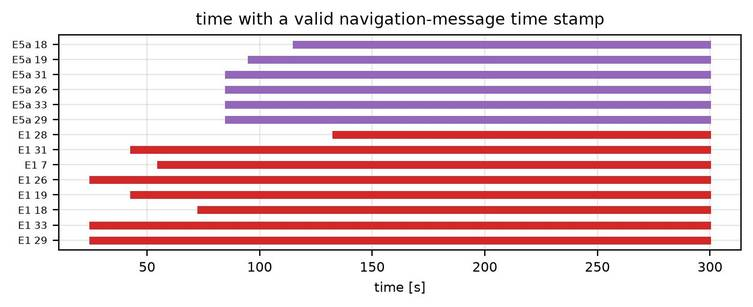
\includegraphics[width=1.0\linewidth]{gnss_sdr/x310_20261024T190000Z/galileo_telemetry.jpg}
  \caption{Telemetry decoder: per band and satellite, when the decoder delivered a valid transmit time (the first one comes after the first complete frame/message).}
\end{figure}

\begin{table}[H]
  \centering
  \footnotesize
  \resizebox{\ifdim\width>\linewidth\linewidth\else\width\fi}{!}{%
  \begin{tabular}{lrrrrr}
    \hline
    \textbf{Band} & \textbf{PRN} & \textbf{Messages decoded} & \textbf{Ephemeris} & \textbf{First valid at [s]} & \textbf{TOW [s]} \\
    \hline
    E1 & 7 & 24 & yes & 54.7 & 586880.0 \\
    E1 & 18 & 22 & yes & 72.7 & 586898.0 \\
    E1 & 19 & 24 & yes & 42.7 & 586868.0 \\
    E1 & 26 & 27 & yes & 24.7 & 586850.0 \\
    E1 & 28 & 16 & yes & 132.7 & 586958.0 \\
    E1 & 29 & 25 & yes & 24.7 & 586850.0 \\
    E1 & 31 & 25 & yes & 42.7 & 586868.0 \\
    E1 & 33 & 26 & yes & 24.7 & 586850.0 \\
    E5a & 18 & 10 & yes & 114.9 & 586940.3 \\
    E5a & 19 & 11 & yes & 94.9 & 586920.3 \\
    E5a & 26 & 12 & yes & 84.9 & 586910.3 \\
    E5a & 29 & 12 & yes & 84.9 & 586910.3 \\
    E5a & 31 & 12 & yes & 84.9 & 586910.3 \\
    E5a & 33 & 12 & yes & 84.9 & 586910.3 \\
    \hline
  \end{tabular}}
  \caption{Telemetry decoder: E1 I/NAV words, E5a F/NAV pages decoded, ephemeris obtained, and the first valid time of week.}
\end{table}

\subsubsection{Observables (Galileo E1 + E5a)}
Pseudorange, carrier phase and Doppler of every channel at common receiver epochs.

\begin{figure}[H]
  \centering
  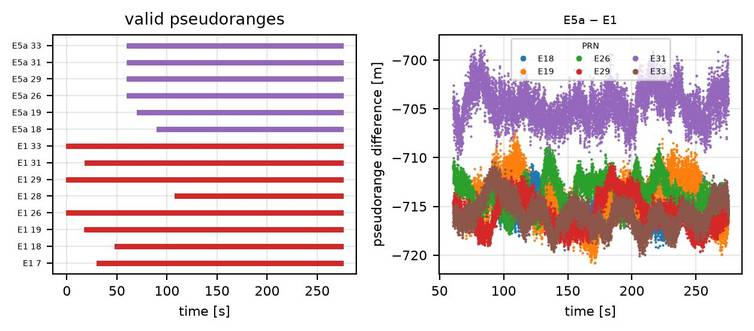
\includegraphics[width=1.0\linewidth]{gnss_sdr/x310_20261024T190000Z/galileo_observables.jpg}
  \caption{Observables: epochs with a valid pseudorange per band and satellite, and the difference between the two bands' pseudoranges of the same satellite (a constant receiver inter-band bias, the same for every satellite, plus the slowly varying ionospheric delay).}
\end{figure}

\begin{table}[H]
  \centering
  \footnotesize
  \resizebox{\ifdim\width>\linewidth\linewidth\else\width\fi}{!}{%
  \begin{tabular}{lrrrrrr}
    \hline
    \textbf{Difference} & \textbf{PRN} & \textbf{Common epochs} & \textbf{of run [\%]} & \textbf{Mean [m]} & \textbf{Std [m]} & \textbf{Drift [m/s]} \\
    \hline
    E5a $-$ E1 & 18 & 9240 & 62 & -715.18 & 1.29 & -0.0008 \\
    E5a $-$ E1 & 19 & 10241 & 68 & -714.24 & 2.20 & -0.0021 \\
    E5a $-$ E1 & 26 & 10728 & 72 & -713.77 & 1.56 & -0.0003 \\
    E5a $-$ E1 & 29 & 10727 & 72 & -715.68 & 1.65 & -0.0031 \\
    E5a $-$ E1 & 31 & 10726 & 72 & -704.59 & 1.77 & 0.0011 \\
    E5a $-$ E1 & 33 & 10727 & 72 & -715.80 & 1.51 & -0.0056 \\
    \hline
  \end{tabular}}
  \caption{Observables: pseudorange difference between the two bands of each satellite at common epochs (similar means = shared receiver bias; std = code noise of both bands).}
\end{table}

\subsubsection{PVT (Galileo E1 + E5a)}
Position from the pseudoranges and the decoded ephemeris, compared with the surveyed antenna position (-23.209433$^\circ$, -45.874875$^\circ$, 596.42~m).

\begin{figure}[H]
  \centering
  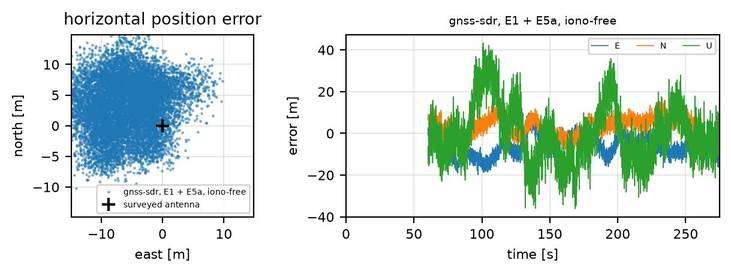
\includegraphics[width=1.0\linewidth]{gnss_sdr/x310_20261024T190000Z/galileo_pvt.jpg}
  \caption{PVT: position error with respect to the surveyed antenna position. gnss-sdr: GNSS-SDR's own RTKLIB solution.}
\end{figure}

\begin{table}[H]
  \centering
  \footnotesize
  \resizebox{\ifdim\width>\linewidth\linewidth\else\width\fi}{!}{%
  \begin{tabular}{l>{\centering\arraybackslash}p{4.2cm}}
    \hline
    \textbf{Solution} & \textbf{gnss-sdr, E1 + E5a, iono-free} \\
    \hline
    Solutions & 10909 \\
    Run with fix [\%] & 79 \\
    Mean E / N / U [m] & -6.0 / 3.2 / 0.0 \\
    Std E / N / U [m] & 4.8 / 4.5 / 13.5 \\
    RMS 2-D [m] & 9.4 \\
    RMS 3-D [m] & 16.4 \\
    95\% horiz. [m] & 15.1 \\
    \hline
  \end{tabular}}
  \caption{PVT: position error statistics with respect to the surveyed antenna (mean = accuracy, std = precision; \% of the run's seconds with a position; gnss-sdr outputs several solutions per second, gnss\_spp\_lib.py computes one per second).}
\end{table}




\subsection{Second record}
\begin{table}[H]
  \centering
  \begin{tabular}{|l|l|l|}
    \hline
    \textbf{Parameter} & \textbf{Channel 0} & \textbf{Channel 1} \\
    \hline
    Start time & \multicolumn{2}{>{\centering\arraybackslash}p{7cm}|}{2026-10-24 19:30:07 UTC} \\
    \hline
    Frequency & 1575.420 MHz (L1) & 1227.600 MHz (L2) \\
    \hline
    Duration & 300.0 s & 300.0 s \\
    \hline
    Sample rate & 4.000 MS/s & 4.000 MS/s \\
    \hline
    Sample type & \multicolumn{2}{>{\centering\arraybackslash}p{7cm}|}{signed complex 16-bit samples (I+Q), little-endian, as received from the X310 (sc16)} \\
    \hline
    Gain & 25.0 dB & 25.0 dB \\
    \hline
    Antenna & RX1 & RX2 \\
    \hline
    File size & 4800.0 MB & 4800.0 MB \\
    \hline
    Samples written & 1,200,000,000 & 1,200,000,000 \\
    \hline
    Lost samples & 0 & 0 \\
    \hline
    Clock source & \multicolumn{2}{>{\centering\arraybackslash}p{7cm}|}{external} \\
    \hline
    Time source & \multicolumn{2}{>{\centering\arraybackslash}p{7cm}|}{internal} \\
    \hline
    Motherboard & \multicolumn{2}{>{\centering\arraybackslash}p{7cm}|}{USRP X310} \\
    \hline
    Daughterboard & TwinRX RX0 & TwinRX RX1 \\
    \hline
    Recorder & \multicolumn{2}{>{\centering\arraybackslash}p{7cm}|}{UHD Python API} \\
    \hline
    GNSS-SDR configuration & \multicolumn{2}{>{\centering\arraybackslash}p{7cm}|}{\texttt{l1ca16bits4msps\_l2c16bits4msps.conf}} \\
    \hline
  \end{tabular}
  \caption{Metadata for recording \texttt{x310\_20261024T193000Z}, captured starting 2026-10-24T19:30:07.284275Z.}
\end{table}

\subsubsection{Signal source}
Raw I/Q samples of each channel analysed within the window [10, 10.5]~s after the start recording instant.

\begin{figure}[H]
  \centering
  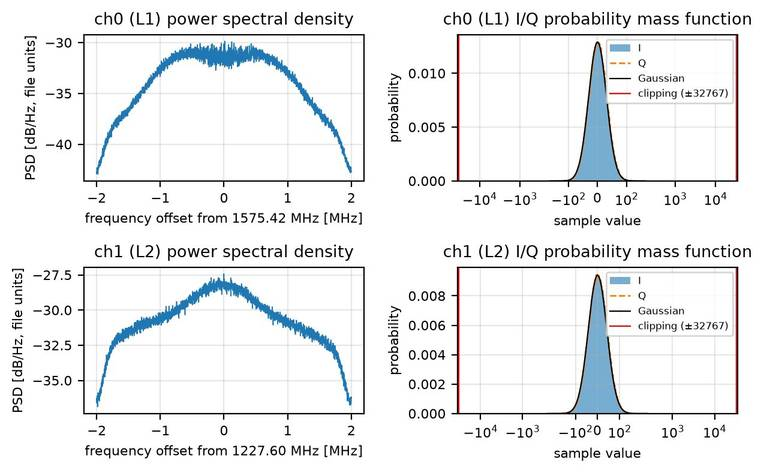
\includegraphics[width=1.0\linewidth]{gnss_sdr/x310_20261024T193000Z/source.jpg}
  \caption{Signal source: power spectral density (the receiver passband over a flat thermal-noise floor; GNSS signals are below the noise, so only interference would stand out) and probability mass functions of the integer I/Q sample values (Gaussian noise, centred, not clipped).}
\end{figure}

\begin{table}[H]
  \centering
  \footnotesize
  \resizebox{\ifdim\width>\linewidth\linewidth\else\width\fi}{!}{%
  \begin{tabular}{l>{\centering\arraybackslash}p{4.2cm}>{\centering\arraybackslash}p{4.2cm}}
    \hline
    \textbf{Channel} & \textbf{ch0} & \textbf{ch1} \\
    \hline
    Frequency [MHz] & 1575.42 & 1227.60 \\
    Rate [MS/s] & 4 & 4 \\
    Format & ci16\_le & ci16\_le \\
    Bytes per complex sample & 4 (2 for I, 2 for Q) & 4 (2 for I, 2 for Q) \\
    Full scale & $\pm$32767 & $\pm$32767 \\
    Gain [dB] & 25 & 25 \\
    Std I / Q & 30.9 / 31.0 & 42.5 / 42.4 \\
    Mean I / Q & -0.15 / 0.08 & -0.17 / -0.04 \\
    Min / max I & -146 / 146 & -216 / 196 \\
    Min / max Q & -152 / 146 & -204 / 217 \\
    Headroom\footnotemark & 1058.6 & 772.1 \\
    Clipped [\%] & 0.000 & 0.000 \\
    Lost samples & 0 & 0 \\
    \hline
  \end{tabular}}
  \caption{Signal source: sample statistics per channel (headroom: how many standard deviations of the noise fit before clipping).}
\end{table}

\footnotetext{Headroom $= A/\sigma$, where $A$ is the full scale of the sample format (127 for 8-bit, 32767 for 16-bit) and $\sigma$ the standard deviation of the I and Q samples together (both in file units, over the analysed window). For Gaussian noise, the fraction of clipped values is $2Q(A/\sigma)$, with $Q$ the Gaussian tail function: e.g. 0.003\,\% at $4.2\sigma$.}

\subsubsection{Signal conditioner}


\begin{table}[H]
  \centering
  \footnotesize
  \resizebox{\ifdim\width>\linewidth\linewidth\else\width\fi}{!}{%
  \begin{tabular}{l>{\centering\arraybackslash}p{4.2cm}>{\centering\arraybackslash}p{4.2cm}}
    \hline
    \textbf{Channel} & \textbf{ch0 (L1 C/A, E1)} & \textbf{ch1 (L2C)} \\
    \hline
    File format & ci16\_le & ci16\_le \\
    Source item type & ishort & ishort \\
    Data type adapter & Ishort\_To\_Complex & Ishort\_To\_Complex \\
    Input filter & Pass\_Through & Pass\_Through \\
    Resampling & Pass\_Through & Pass\_Through \\
    Rate [MS/s] & 4 $\to$ 4 & 4 $\to$ 4 \\
    \hline
  \end{tabular}}
  \caption{Signal conditioner: recorded format and rate to gnss-sdr's internal \texttt{gr\_complex} stream; both bands are read in lockstep by one \texttt{Multichannel\_File\_Signal\_Source}.}
\end{table}

\subsubsection{Acquisition}
Two-dimensional search over code delay and Doppler (one channel per band dumped; the others behave alike).

\begin{figure}[H]
  \centering
  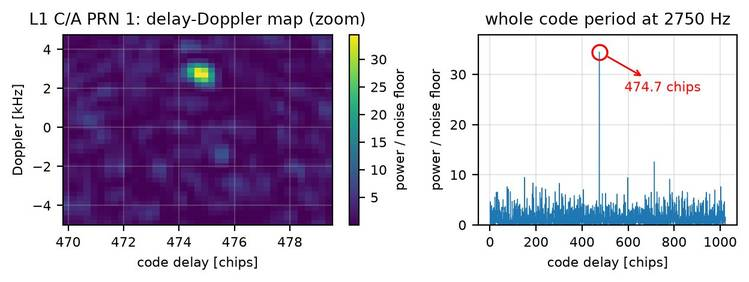
\includegraphics[width=1.0\linewidth]{gnss_sdr/x310_20261024T193000Z/acq_1C.jpg}
  \caption{Acquisition, L1 C/A: delay--Doppler search of PRN 1; one sharp peak (test statistic 49 vs threshold 44) at 2750~Hz and 474.7~chips.}
\end{figure}

\begin{figure}[H]
  \centering
  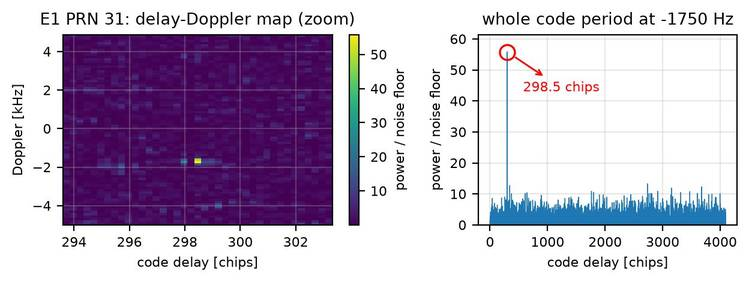
\includegraphics[width=1.0\linewidth]{gnss_sdr/x310_20261024T193000Z/acq_1B.jpg}
  \caption{Acquisition, E1: delay--Doppler search of PRN 31; one sharp peak (test statistic 79 vs threshold 48) at -1750~Hz and 298.5~chips.}
\end{figure}

\begin{table}[H]
  \centering
  \footnotesize
  \resizebox{\ifdim\width>\linewidth\linewidth\else\width\fi}{!}{%
  \begin{tabular}{lrrrr}
    \hline
    \textbf{Band} & \textbf{Attempts} & \textbf{Detections} & \textbf{Detected PRNs} & \textbf{Best statistic / threshold\footnotemark} \\
    \hline
    L1 C/A & 485 & 1 & 1 & 1.1 \\
    L2C & \multicolumn{4}{l}{not dumped (search grid too large); acquired satellites: see the tracking table} \\
    E1 & 4 & 1 & 31 & 1.6 \\
    \hline
  \end{tabular}}
  \caption{Acquisition: search attempts of the dumped channel. Attempts on satellites that are not in view (or do not broadcast that signal, e.g. older GPS satellites on L5/L2C) are rejected below the threshold.}
\end{table}

\footnotetext{Margin of the band's strongest detection: the largest acquisition test statistic among the detected attempts (the correlation peak of the delay--Doppler grid, normalised by the power of the input samples searched, i.e. the noise power, since GNSS signals are below the noise) divided by the detection threshold, which GNSS-SDR derives from the configured probability of false alarm. A value of 1 is right at the detection limit; e.g. 2.5 means the peak cleared the threshold 2.5 times over.}

\subsubsection{Tracking}


\begin{figure}[H]
  \centering
  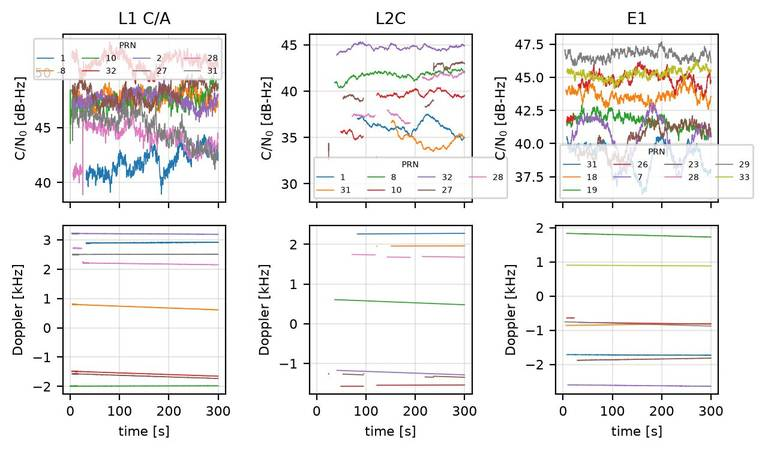
\includegraphics[width=1.0\linewidth]{gnss_sdr/x310_20261024T193000Z/tracking.jpg}
  \caption{Tracking: carrier-to-noise density ratio and carrier Doppler per satellite, while phase-locked (smooth Doppler curves = loops following the real satellite motion).}
\end{figure}

\begin{figure}[H]
  \centering
  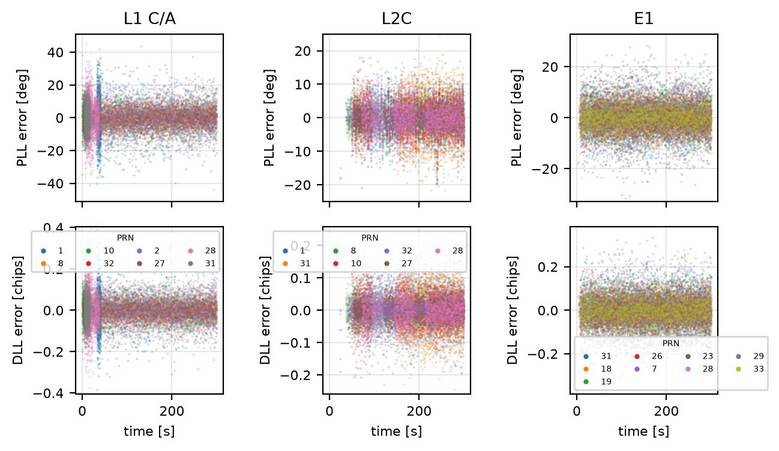
\includegraphics[width=1.0\linewidth]{gnss_sdr/x310_20261024T193000Z/tracking_errors.jpg}
  \caption{Tracking: loop errors per satellite while phase-locked, i.e. the discriminator outputs that the loops drive to zero: PLL carrier-phase error (degrees) and DLL code-delay error (chips) of every correlation. Noise centred on zero = clean tracking; its spread grows as C/N$_0$ drops, and jumps would mark cycle slips or a loop losing lock.}
\end{figure}

\begin{figure}[H]
  \centering
  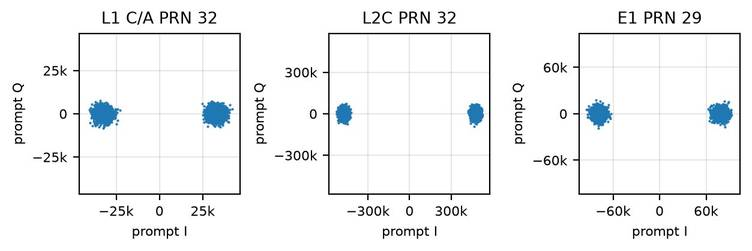
\includegraphics[width=1.0\linewidth]{gnss_sdr/x310_20261024T193000Z/tracking_iq.jpg}
  \caption{Tracking: prompt correlator outputs of the strongest satellite per band. Two tight clusters on one axis (the $\pm1$ data bits; GNSS-SDR's L5 tracking puts the data component on the Q axis), or, for the dataless pilots tracked for Galileo (E1-C, E5a-Q), the $\pm1$ chips of their secondary code, mean the PLL is phase-locked; a ring would mean it is not. \texttt{Prompt\_I}/\texttt{Prompt\_Q} are 32-bit floats (sums of the samples over one integration period, in file units): they never clip, only overflowing beyond $\pm 3.4\times10^{38}$, far above the $N\cdot\text{full scale}\cdot\sqrt{2}$ a sum of $N$ samples can reach.}
\end{figure}

\begin{table}[H]
  \centering
  \footnotesize
  \resizebox{\ifdim\width>\linewidth\linewidth\else\width\fi}{!}{%
  \begin{tabular}{lrrrrrrrr}
    \hline
    \textbf{Band} & \textbf{Ch.} & \textbf{PRN} & \textbf{Median C/N$_0$ [dB-Hz]} & \textbf{Phase-locked [\%]} & \textbf{Losses of lock} & \textbf{Tracked [s]} & \textbf{PLL error std [deg]} & \textbf{DLL error std [chips]} \\
    \hline
    L1 C/A & 0 & 1 & 41.0 & 88 & 0 & 270 & 12.5 & 0.095 \\
    L1 C/A & 1 & 8 & 47.8 & 95 & 0 & 297 & 5.9 & 0.047 \\
    L1 C/A & 2 & 10 & 47.2 & 100 & 0 & 300 & 6.4 & 0.049 \\
    L1 C/A & 3 & 32 & 51.3 & 96 & 0 & 298 & 4.0 & 0.031 \\
    L1 C/A & 4 & 2 & 47.4 & 96 & 0 & 298 & 6.1 & 0.046 \\
    L1 C/A & 5 & 27 & 48.2 & 92 & 0 & 298 & 5.6 & 0.043 \\
    L1 C/A & 6 & 28 & 43.1 & 90 & 1 & 296 & 10.8 & 0.083 \\
    L1 C/A & 7 & 31 & 45.9 & 100 & 0 & 295 & 7.8 & 0.061 \\
    L2C & 8 & 1 & 36.2 & 86 & 0 & 253 & 5.3 & 0.060 \\
    L2C & 9 & 31 & 35.0 & 55 & 3 & 276 & 6.6 & 0.069 \\
    L2C & 10 & 8 & 41.8 & 95 & 0 & 277 & 3.3 & 0.030 \\
    L2C & 11 & 10 & 39.5 & 81 & 1 & 276 & 4.3 & 0.045 \\
    L2C & 12 & 32 & 44.7 & 94 & 0 & 276 & 2.7 & 0.022 \\
    L2C & 14 & 27 & 39.6 & 45 & 3 & 276 & 5.6 & 0.036 \\
    L2C & 15 & 28 & 37.7 & 71 & 2 & 252 & 4.4 & 0.042 \\
    E1 & 16 & 31 & 39.2 & 98 & 0 & 298 & 8.5 & 0.097 \\
    E1 & 17 & 18 & 43.6 & 99 & 0 & 299 & 4.8 & 0.056 \\
    E1 & 18 & 19 & 41.7 & 98 & 0 & 299 & 6.0 & 0.070 \\
    E1 & 19 & 26 & 44.9 & 97 & 1 & 294 & 4.4 & 0.049 \\
    E1 & 20 & 7 & 40.8 & 98 & 0 & 296 & 6.9 & 0.079 \\
    E1 & 21 & 23 & 40.6 & 99 & 1 & 275 & 7.0 & 0.081 \\
    E1 & 21 & 28 & 42.5 & 0 & 1 & 21 & -- & -- \\
    E1 & 22 & 29 & 46.6 & 100 & 0 & 298 & 3.4 & 0.040 \\
    E1 & 23 & 33 & 45.3 & 98 & 0 & 297 & 3.5 & 0.041 \\
    \hline
  \end{tabular}}
  \caption{Tracking: per channel and satellite (phase-locked: carrier lock test $> 0.8$; loop error standard deviations while phase-locked).}
\end{table}

\subsubsection{Telemetry decoder}


\begin{figure}[H]
  \centering
  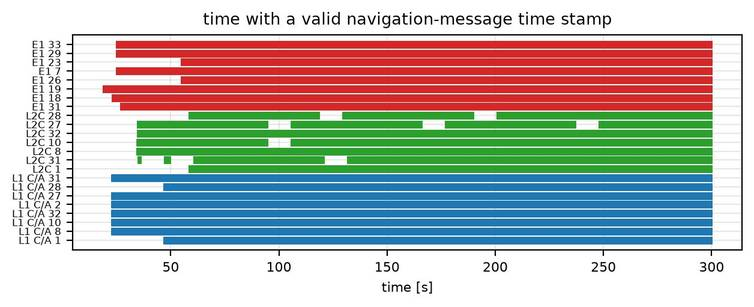
\includegraphics[width=1.0\linewidth]{gnss_sdr/x310_20261024T193000Z/telemetry.jpg}
  \caption{Telemetry decoder: per band and satellite, when the decoder delivered a valid transmit time (the first one comes after the first complete frame/message).}
\end{figure}

\begin{table}[H]
  \centering
  \footnotesize
  \resizebox{\ifdim\width>\linewidth\linewidth\else\width\fi}{!}{%
  \begin{tabular}{lrrrrr}
    \hline
    \textbf{Band} & \textbf{PRN} & \textbf{Messages decoded} & \textbf{Ephemeris} & \textbf{First valid at [s]} & \textbf{TOW [s]} \\
    \hline
    E1 & 7 & 26 & yes & 24.9 & 588650.0 \\
    E1 & 18 & 27 & yes & 22.8 & 588648.0 \\
    E1 & 19 & 27 & yes & 18.8 & 588644.0 \\
    E1 & 23 & 24 & yes & 54.9 & 588680.0 \\
    E1 & 26 & 24 & yes & 54.8 & 588680.0 \\
    E1 & 29 & 26 & yes & 24.8 & 588650.0 \\
    E1 & 31 & 26 & yes & 26.9 & 588652.0 \\
    E1 & 33 & 26 & yes & 24.8 & 588650.0 \\
    L1 C/A & 1 & 43 & yes & 46.8 & 588672.0 \\
    L1 C/A & 2 & 47 & yes & 22.8 & 588648.0 \\
    L1 C/A & 8 & 47 & yes & 22.8 & 588648.0 \\
    L1 C/A & 10 & 46 & yes & 22.8 & 588648.0 \\
    L1 C/A & 27 & 47 & yes & 22.8 & 588648.0 \\
    L1 C/A & 28 & 42 & yes & 46.8 & 588672.0 \\
    L1 C/A & 31 & 47 & yes & 22.8 & 588648.0 \\
    L1 C/A & 32 & 47 & yes & 22.8 & 588648.0 \\
    L2C & 1 & 14 & yes & 58.4 & 0.0 \\
    L2C & 8 & 13 & yes & 34.4 & 0.0 \\
    L2C & 10 & 9 & yes & 34.5 & 0.0 \\
    L2C & 27 & 2 & no & 34.7 & 0.0 \\
    L2C & 28 & 5 & yes & 58.5 & 0.0 \\
    L2C & 31 & 8 & yes & 35.0 & 0.0 \\
    L2C & 32 & 13 & yes & 34.5 & 0.0 \\
    \hline
  \end{tabular}}
  \caption{Telemetry decoder: L1 C/A LNAV subframes, L2C CNAV messages, E1 I/NAV words decoded, ephemeris obtained, and the first valid time of week.}
\end{table}

\subsubsection{Observables}
Pseudorange, carrier phase and Doppler of every channel at common receiver epochs.

\begin{figure}[H]
  \centering
  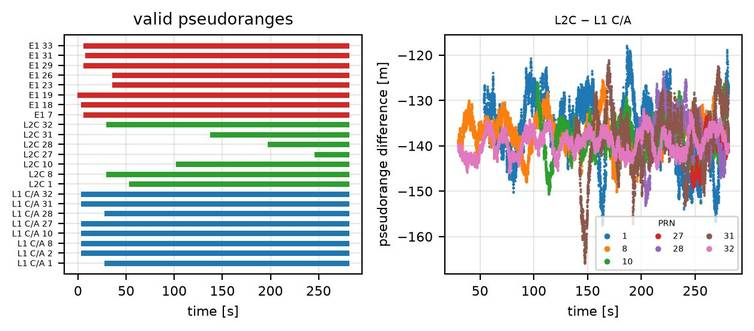
\includegraphics[width=1.0\linewidth]{gnss_sdr/x310_20261024T193000Z/observables.jpg}
  \caption{Observables: epochs with a valid pseudorange per band and satellite, and the difference between the two bands' pseudoranges of the same satellite (a constant receiver inter-band bias, the same for every satellite, plus the slowly varying ionospheric delay).}
\end{figure}

\begin{table}[H]
  \centering
  \footnotesize
  \resizebox{\ifdim\width>\linewidth\linewidth\else\width\fi}{!}{%
  \begin{tabular}{lrrrrrr}
    \hline
    \textbf{Difference} & \textbf{PRN} & \textbf{Common epochs} & \textbf{of run [\%]} & \textbf{Mean [m]} & \textbf{Std [m]} & \textbf{Drift [m/s]} \\
    \hline
    L2C $-$ L1 C/A & 1 & 11364 & 76 & -136.67 & 7.21 & -0.0353 \\
    L2C $-$ L1 C/A & 8 & 12562 & 84 & -137.27 & 3.68 & -0.0021 \\
    L2C $-$ L1 C/A & 10 & 8932 & 60 & -138.51 & 4.05 & -0.0000 \\
    L2C $-$ L1 C/A & 27 & 1736 & 12 & -140.56 & 4.07 & 0.1949 \\
    L2C $-$ L1 C/A & 28 & 4170 & 28 & -137.26 & 5.58 & -0.0237 \\
    L2C $-$ L1 C/A & 31 & 7158 & 48 & -138.45 & 7.12 & 0.0509 \\
    L2C $-$ L1 C/A & 32 & 12556 & 84 & -139.30 & 2.55 & 0.0083 \\
    \hline
  \end{tabular}}
  \caption{Observables: pseudorange difference between the two bands of each satellite at common epochs (similar means = shared receiver bias; std = code noise of both bands).}
\end{table}

\subsubsection{PVT}
Position from the pseudoranges and the decoded ephemeris, compared with the surveyed antenna position (-23.209433$^\circ$, -45.874875$^\circ$, 596.42~m).

\begin{figure}[H]
  \centering
  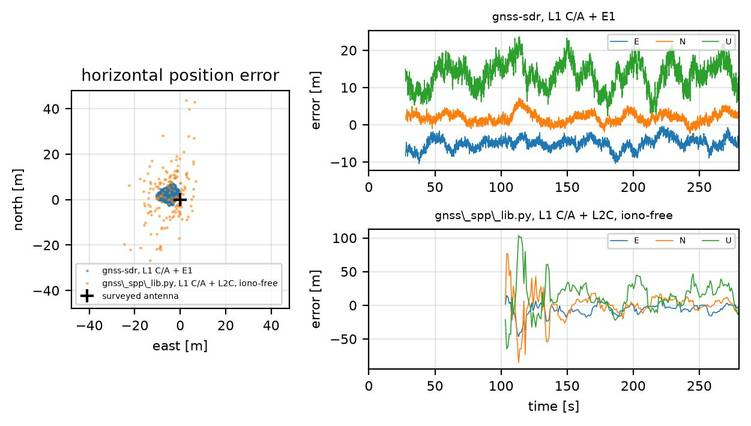
\includegraphics[width=1.0\linewidth]{gnss_sdr/x310_20261024T193000Z/pvt.jpg}
  \caption{PVT: position error with respect to the surveyed antenna position. gnss-sdr: GNSS-SDR's own RTKLIB solution (single frequency, broadcast ionosphere model). gnss\_spp\_lib.py: computed from gnss-sdr's observables and decoded GPS ephemeris, removing the ionospheric delay with the second band (pseudoranges carrier-smoothed over 100~s).}
\end{figure}

\begin{figure}[H]
  \centering
  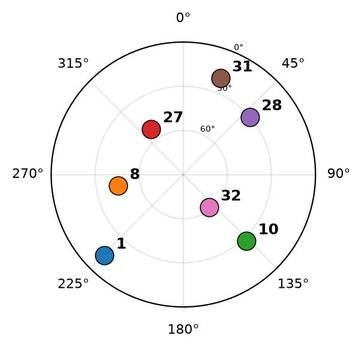
\includegraphics[width=0.45\linewidth]{gnss_sdr/x310_20261024T193000Z/skyplot.jpg}
  \caption{PVT: sky plot of the GPS satellites in the gnss\_spp\_lib.py dual-frequency solution (azimuth, elevation) during the recording.}
\end{figure}

\begin{table}[H]
  \centering
  \footnotesize
  \resizebox{\ifdim\width>\linewidth\linewidth\else\width\fi}{!}{%
  \begin{tabular}{l>{\centering\arraybackslash}p{4.2cm}>{\centering\arraybackslash}p{4.2cm}}
    \hline
    \textbf{Solution} & \textbf{gnss-sdr, L1 C/A + E1} & \textbf{gnss\_spp\_lib.py, L1 C/A + L2C, iono-free} \\
    \hline
    Solutions & 13152 & 178 \\
    Run with fix [\%] & 91 & 64 \\
    Mean E / N / U [m] & -5.0 / 1.9 / 13.3 & -6.4 / 0.3 / 13.9 \\
    Std E / N / U [m] & 1.6 / 1.4 / 3.7 & 9.2 / 19.9 / 24.5 \\
    RMS 2-D [m] & 5.8 & 22.8 \\
    RMS 3-D [m] & 15.0 & 36.2 \\
    95\% horiz. [m] & 8.2 & 55.6 \\
    \hline
  \end{tabular}}
  \caption{PVT: position error statistics with respect to the surveyed antenna (mean = accuracy, std = precision; \% of the run's seconds with a position; gnss-sdr outputs several solutions per second, gnss\_spp\_lib.py computes one per second).}
\end{table}




\section{Records on 25/10/2026}

\subsection{First record}
\begin{table}[H]
  \centering
  \begin{tabular}{|l|l|l|}
    \hline
    \textbf{Parameter} & \textbf{Channel 0} & \textbf{Channel 1} \\
    \hline
    Start time & \multicolumn{2}{>{\centering\arraybackslash}p{7cm}|}{2026-10-25 19:00:07 UTC} \\
    \hline
    Frequency & 1575.420 MHz (L1) & 1176.450 MHz (L5) \\
    \hline
    Duration & 300.0 s & 300.0 s \\
    \hline
    Sample rate & 4.000 MS/s & 20.000 MS/s \\
    \hline
    Sample type & \multicolumn{2}{>{\centering\arraybackslash}p{7cm}|}{signed complex 8-bit samples (I+Q), converted on the host from the X310's sc16} \\
    \hline
    Gain & 25.0 dB & 25.0 dB \\
    \hline
    Antenna & RX1 & RX2 \\
    \hline
    File size & 2400.0 MB & 12000.0 MB \\
    \hline
    Samples written & 1,200,000,000 & 6,000,000,000 \\
    \hline
    Lost samples & 0 & 1134464 \\
    \hline
    Clock source & \multicolumn{2}{>{\centering\arraybackslash}p{7cm}|}{external} \\
    \hline
    Time source & \multicolumn{2}{>{\centering\arraybackslash}p{7cm}|}{internal} \\
    \hline
    Motherboard & \multicolumn{2}{>{\centering\arraybackslash}p{7cm}|}{USRP X310} \\
    \hline
    Daughterboard & TwinRX RX0 & TwinRX RX1 \\
    \hline
    Recorder & \multicolumn{2}{>{\centering\arraybackslash}p{7cm}|}{UHD Python API} \\
    \hline
    GNSS-SDR configuration & \multicolumn{2}{>{\centering\arraybackslash}p{7cm}|}{\texttt{l1ca8bits4msps\_l5\_8bits20msps.conf}, \texttt{e1\_8bits4msps\_e5a\_8bits20msps.conf}} \\
    \hline
  \end{tabular}
  \caption{Metadata for recording \texttt{x310\_20261025T190000Z}, captured starting 2026-10-25T19:00:07.043233Z.}
\end{table}

\subsubsection{Signal source}
Raw I/Q samples of each channel analysed within the window [10, 10.5]~s after the start recording instant.

\begin{figure}[H]
  \centering
  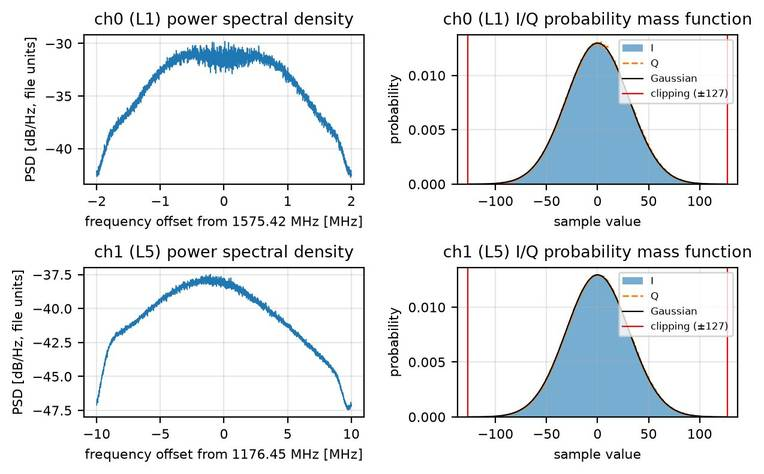
\includegraphics[width=1.0\linewidth]{gnss_sdr/x310_20261025T190000Z/source.jpg}
  \caption{Signal source: power spectral density (the receiver passband over a flat thermal-noise floor; GNSS signals are below the noise, so only interference would stand out) and probability mass functions of the integer I/Q sample values (Gaussian noise, centred, not clipped).}
\end{figure}

\begin{table}[H]
  \centering
  \footnotesize
  \resizebox{\ifdim\width>\linewidth\linewidth\else\width\fi}{!}{%
  \begin{tabular}{l>{\centering\arraybackslash}p{4.2cm}>{\centering\arraybackslash}p{4.2cm}}
    \hline
    \textbf{Channel} & \textbf{ch0} & \textbf{ch1} \\
    \hline
    Frequency [MHz] & 1575.42 & 1176.45 \\
    Rate [MS/s] & 4 & 20 \\
    Format & ci8 & ci8 \\
    Bytes per complex sample & 2 (1 for I, 1 for Q) & 2 (1 for I, 1 for Q) \\
    Full scale & $\pm$127 & $\pm$127 \\
    Gain [dB] & 25 & 25 \\
    Std I / Q & 30.7 / 30.7 & 30.8 / 30.8 \\
    Mean I / Q & -0.19 / 0.06 & -0.02 / 0.01 \\
    Min / max I & -127 / 127 & -127 / 127 \\
    Min / max Q & -127 / 127 & -127 / 127 \\
    Headroom\footnotemark & 4.1 & 4.1 \\
    Clipped [\%] & 0.004 & 0.004 \\
    Lost samples & 0 & 1,134,464 \\
    \hline
  \end{tabular}}
  \caption{Signal source: sample statistics per channel (headroom: how many standard deviations of the noise fit before clipping).}
\end{table}

\footnotetext{Headroom $= A/\sigma$, where $A$ is the full scale of the sample format (127 for 8-bit, 32767 for 16-bit) and $\sigma$ the standard deviation of the I and Q samples together (both in file units, over the analysed window). For Gaussian noise, the fraction of clipped values is $2Q(A/\sigma)$, with $Q$ the Gaussian tail function: e.g. 0.003\,\% at $4.2\sigma$.}

\subsubsection{Signal conditioner}


\begin{table}[H]
  \centering
  \footnotesize
  \resizebox{\ifdim\width>\linewidth\linewidth\else\width\fi}{!}{%
  \begin{tabular}{l>{\centering\arraybackslash}p{4.2cm}>{\centering\arraybackslash}p{4.2cm}}
    \hline
    \textbf{Channel} & \textbf{ch0 (L1 C/A)} & \textbf{ch1 (L5)} \\
    \hline
    File format & ci8 & ci8 \\
    Source item type & ibyte & ibyte \\
    Data type adapter & Ibyte\_To\_Complex & Ibyte\_To\_Complex \\
    Input filter & Pass\_Through & Pass\_Through \\
    Resampling & $\times$5 zero-order hold, offline (\texttt{upsample\_iq.py}) & Pass\_Through \\
    Rate [MS/s] & 4 $\to$ 20 & 20 $\to$ 20 \\
    \hline
  \end{tabular}}
  \caption{Signal conditioner: recorded format and rate to gnss-sdr's internal \texttt{gr\_complex} stream; both bands are read in lockstep by one \texttt{Multichannel\_File\_Signal\_Source}.}
\end{table}

\subsubsection{Acquisition}
Two-dimensional search over code delay and Doppler (one channel per band dumped; the others behave alike).

\begin{figure}[H]
  \centering
  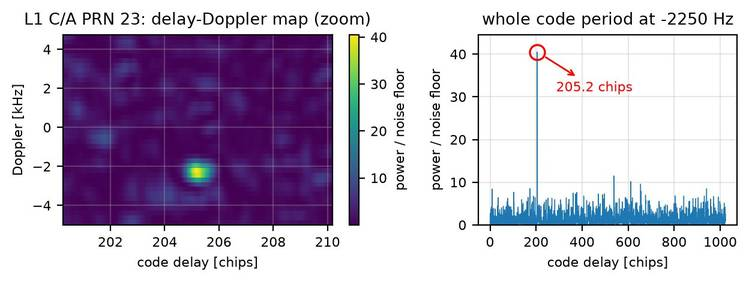
\includegraphics[width=1.0\linewidth]{gnss_sdr/x310_20261025T190000Z/acq_1C.jpg}
  \caption{Acquisition, L1 C/A: delay--Doppler search of PRN 23; one sharp peak (test statistic 55 vs threshold 47) at -2250~Hz and 205.2~chips.}
\end{figure}

\begin{table}[H]
  \centering
  \footnotesize
  \resizebox{\ifdim\width>\linewidth\linewidth\else\width\fi}{!}{%
  \begin{tabular}{lrrrr}
    \hline
    \textbf{Band} & \textbf{Attempts} & \textbf{Detections} & \textbf{Detected PRNs} & \textbf{Best statistic / threshold\footnotemark} \\
    \hline
    L1 C/A & 3 & 1 & 23 & 1.2 \\
    L5 & 13137 & 0 & -- & -- \\
    \hline
  \end{tabular}}
  \caption{Acquisition: search attempts of the dumped channel. Attempts on satellites that are not in view (or do not broadcast that signal, e.g. older GPS satellites on L5/L2C) are rejected below the threshold.}
\end{table}

\footnotetext{Margin of the band's strongest detection: the largest acquisition test statistic among the detected attempts (the correlation peak of the delay--Doppler grid, normalised by the power of the input samples searched, i.e. the noise power, since GNSS signals are below the noise) divided by the detection threshold, which GNSS-SDR derives from the configured probability of false alarm. A value of 1 is right at the detection limit; e.g. 2.5 means the peak cleared the threshold 2.5 times over.}

\subsubsection{Tracking}


\begin{figure}[H]
  \centering
  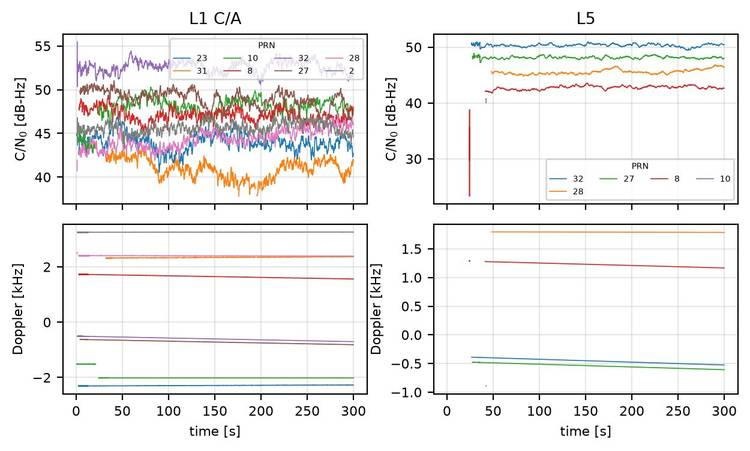
\includegraphics[width=1.0\linewidth]{gnss_sdr/x310_20261025T190000Z/tracking.jpg}
  \caption{Tracking: carrier-to-noise density ratio and carrier Doppler per satellite, while phase-locked (smooth Doppler curves = loops following the real satellite motion).}
\end{figure}

\begin{figure}[H]
  \centering
  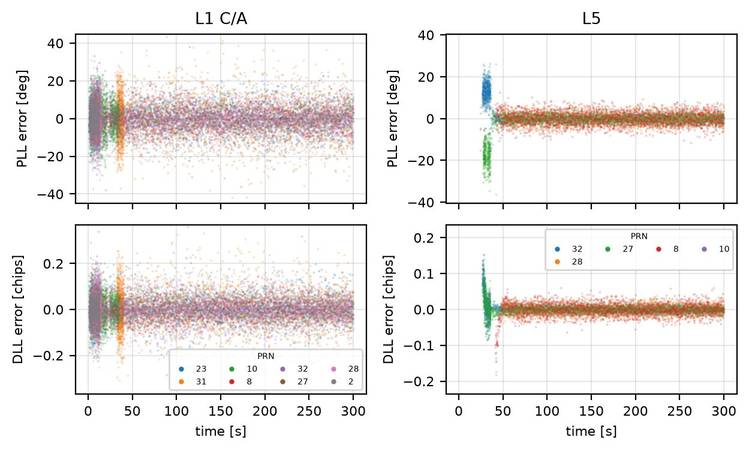
\includegraphics[width=1.0\linewidth]{gnss_sdr/x310_20261025T190000Z/tracking_errors.jpg}
  \caption{Tracking: loop errors per satellite while phase-locked, i.e. the discriminator outputs that the loops drive to zero: PLL carrier-phase error (degrees) and DLL code-delay error (chips) of every correlation. Noise centred on zero = clean tracking; its spread grows as C/N$_0$ drops, and jumps would mark cycle slips or a loop losing lock.}
\end{figure}

\begin{figure}[H]
  \centering
  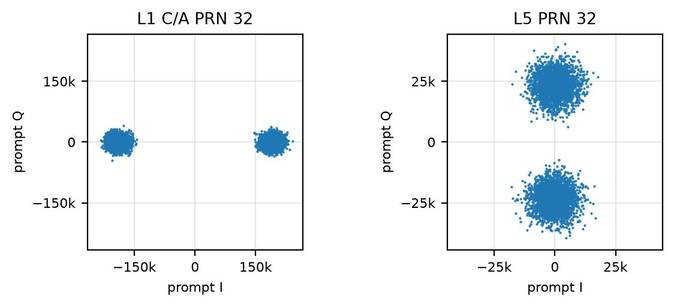
\includegraphics[width=1.0\linewidth]{gnss_sdr/x310_20261025T190000Z/tracking_iq.jpg}
  \caption{Tracking: prompt correlator outputs of the strongest satellite per band. Two tight clusters on one axis (the $\pm1$ data bits; GNSS-SDR's L5 tracking puts the data component on the Q axis), or, for the dataless pilots tracked for Galileo (E1-C, E5a-Q), the $\pm1$ chips of their secondary code, mean the PLL is phase-locked; a ring would mean it is not. \texttt{Prompt\_I}/\texttt{Prompt\_Q} are 32-bit floats (sums of the samples over one integration period, in file units): they never clip, only overflowing beyond $\pm 3.4\times10^{38}$, far above the $N\cdot\text{full scale}\cdot\sqrt{2}$ a sum of $N$ samples can reach.}
\end{figure}

\begin{table}[H]
  \centering
  \footnotesize
  \resizebox{\ifdim\width>\linewidth\linewidth\else\width\fi}{!}{%
  \begin{tabular}{lrrrrrrrr}
    \hline
    \textbf{Band} & \textbf{Ch.} & \textbf{PRN} & \textbf{Median C/N$_0$ [dB-Hz]} & \textbf{Phase-locked [\%]} & \textbf{Losses of lock} & \textbf{Tracked [s]} & \textbf{PLL error std [deg]} & \textbf{DLL error std [chips]} \\
    \hline
    L1 C/A & 0 & 23 & 43.9 & 94 & 0 & 299 & 9.2 & 0.067 \\
    L1 C/A & 1 & 31 & 41.8 & 84 & 0 & 271 & 12.4 & 0.094 \\
    L1 C/A & 2 & 10 & 46.9 & 97 & 1 & 297 & 7.5 & 0.054 \\
    L1 C/A & 3 & 8 & 47.6 & 96 & 0 & 298 & 6.1 & 0.046 \\
    L1 C/A & 4 & 32 & 52.5 & 100 & 0 & 299 & 3.6 & 0.025 \\
    L1 C/A & 5 & 27 & 49.7 & 88 & 0 & 299 & 4.9 & 0.036 \\
    L1 C/A & 6 & 28 & 43.3 & 93 & 0 & 299 & 9.4 & 0.069 \\
    L1 C/A & 7 & 2 & 45.5 & 100 & 0 & 299 & 7.5 & 0.055 \\
    L5 & 9 & 32 & 50.4 & 95 & 0 & 275 & 6.4 & 0.026 \\
    L5 & 10 & 28 & 45.3 & 68 & 0 & 272 & 2.5 & 0.013 \\
    L5 & 11 & 27 & 48.2 & 86 & 0 & 275 & 7.2 & 0.021 \\
    L5 & 14 & 8 & 42.7 & 69 & 0 & 276 & 4.7 & 0.031 \\
    L5 & 15 & 10 & 28.8 & 0 & 1 & 16 & 48.3 & 0.070 \\
    \hline
  \end{tabular}}
  \caption{Tracking: per channel and satellite (phase-locked: carrier lock test $> 0.8$; loop error standard deviations while phase-locked).}
\end{table}

\subsubsection{Telemetry decoder}


\begin{figure}[H]
  \centering
  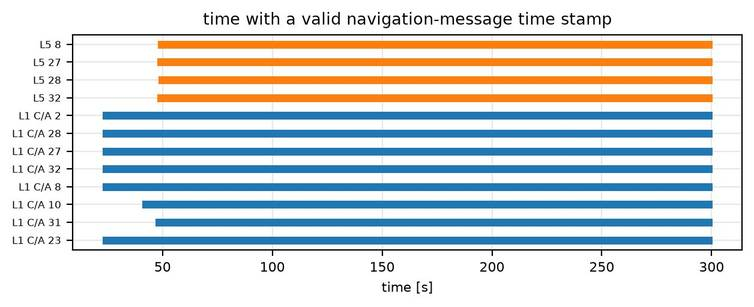
\includegraphics[width=1.0\linewidth]{gnss_sdr/x310_20261025T190000Z/telemetry.jpg}
  \caption{Telemetry decoder: per band and satellite, when the decoder delivered a valid transmit time (the first one comes after the first complete frame/message).}
\end{figure}

\begin{table}[H]
  \centering
  \footnotesize
  \resizebox{\ifdim\width>\linewidth\linewidth\else\width\fi}{!}{%
  \begin{tabular}{lrrrrr}
    \hline
    \textbf{Band} & \textbf{PRN} & \textbf{Messages decoded} & \textbf{Ephemeris} & \textbf{First valid at [s]} & \textbf{TOW [s]} \\
    \hline
    L1 C/A & 2 & 47 & yes & 23.0 & 68448.0 \\
    L1 C/A & 8 & 47 & yes & 23.0 & 68448.0 \\
    L1 C/A & 10 & 44 & yes & 41.0 & 68466.0 \\
    L1 C/A & 23 & 46 & yes & 23.0 & 68448.0 \\
    L1 C/A & 27 & 47 & yes & 23.0 & 68448.0 \\
    L1 C/A & 28 & 47 & yes & 23.0 & 68448.0 \\
    L1 C/A & 31 & 41 & yes & 47.0 & 68472.0 \\
    L1 C/A & 32 & 47 & yes & 23.0 & 68448.0 \\
    L5 & 8 & 25 & yes & 48.2 & 68473.1 \\
    L5 & 27 & 26 & yes & 47.8 & 68472.8 \\
    L5 & 28 & 32 & yes & 48.4 & 68473.4 \\
    L5 & 32 & 26 & yes & 47.8 & 68472.8 \\
    \hline
  \end{tabular}}
  \caption{Telemetry decoder: L1 C/A LNAV subframes, L5 CNAV messages decoded, ephemeris obtained, and the first valid time of week.}
\end{table}

\subsubsection{Observables}
Pseudorange, carrier phase and Doppler of every channel at common receiver epochs.

\begin{figure}[H]
  \centering
  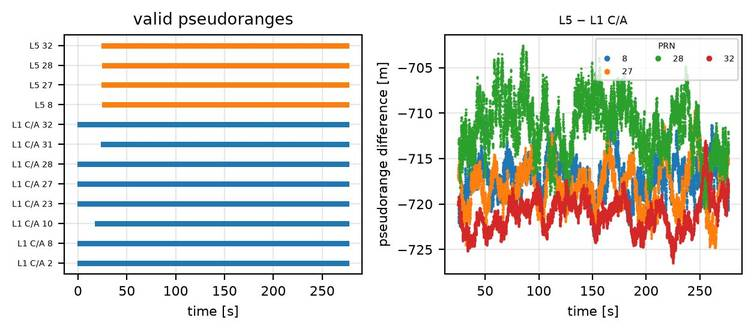
\includegraphics[width=1.0\linewidth]{gnss_sdr/x310_20261025T190000Z/observables.jpg}
  \caption{Observables: epochs with a valid pseudorange per band and satellite, and the difference between the two bands' pseudoranges of the same satellite (a constant receiver inter-band bias, the same for every satellite, plus the slowly varying ionospheric delay).}
\end{figure}

\begin{table}[H]
  \centering
  \footnotesize
  \resizebox{\ifdim\width>\linewidth\linewidth\else\width\fi}{!}{%
  \begin{tabular}{lrrrrrr}
    \hline
    \textbf{Difference} & \textbf{PRN} & \textbf{Common epochs} & \textbf{of run [\%]} & \textbf{Mean [m]} & \textbf{Std [m]} & \textbf{Drift [m/s]} \\
    \hline
    L5 $-$ L1 C/A & 8 & 12423 & 83 & -716.96 & 2.04 & 0.0011 \\
    L5 $-$ L1 C/A & 27 & 12441 & 83 & -718.12 & 2.55 & 0.0021 \\
    L5 $-$ L1 C/A & 28 & 12412 & 83 & -711.59 & 3.06 & -0.0100 \\
    L5 $-$ L1 C/A & 32 & 12442 & 83 & -721.11 & 1.85 & 0.0058 \\
    \hline
  \end{tabular}}
  \caption{Observables: pseudorange difference between the two bands of each satellite at common epochs (similar means = shared receiver bias; std = code noise of both bands).}
\end{table}

\subsubsection{PVT}
Position from the pseudoranges and the decoded ephemeris, compared with the surveyed antenna position (-23.209433$^\circ$, -45.874875$^\circ$, 596.42~m).

\begin{figure}[H]
  \centering
  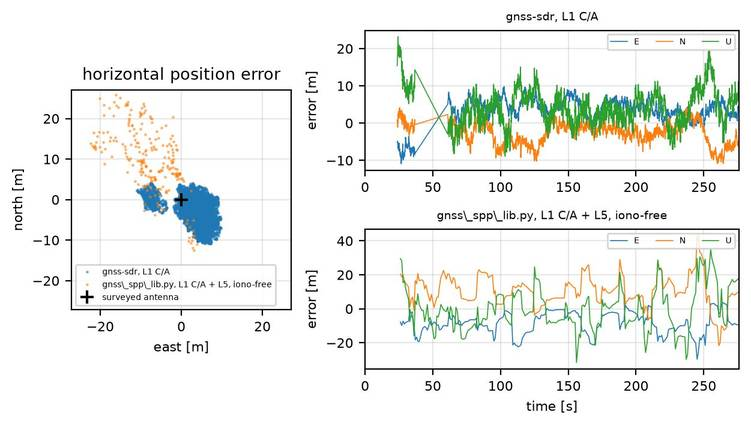
\includegraphics[width=1.0\linewidth]{gnss_sdr/x310_20261025T190000Z/pvt.jpg}
  \caption{PVT: position error with respect to the surveyed antenna position. gnss-sdr: GNSS-SDR's own RTKLIB solution (single frequency, broadcast ionosphere model). gnss\_spp\_lib.py: computed from gnss-sdr's observables and decoded GPS ephemeris, removing the ionospheric delay with the second band (pseudoranges carrier-smoothed over 100~s).}
\end{figure}

\begin{figure}[H]
  \centering
  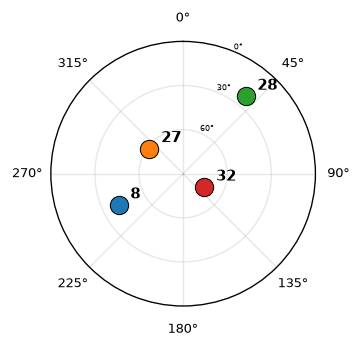
\includegraphics[width=0.45\linewidth]{gnss_sdr/x310_20261025T190000Z/skyplot.jpg}
  \caption{PVT: sky plot of the GPS satellites in the gnss\_spp\_lib.py dual-frequency solution (azimuth, elevation) during the recording.}
\end{figure}

\begin{table}[H]
  \centering
  \footnotesize
  \resizebox{\ifdim\width>\linewidth\linewidth\else\width\fi}{!}{%
  \begin{tabular}{l>{\centering\arraybackslash}p{4.2cm}>{\centering\arraybackslash}p{4.2cm}}
    \hline
    \textbf{Solution} & \textbf{gnss-sdr, L1 C/A} & \textbf{gnss\_spp\_lib.py, L1 C/A + L5, iono-free} \\
    \hline
    Solutions & 11859 & 247 \\
    Run with fix [\%] & 84 & 89 \\
    Mean E / N / U [m] & 3.5 / -2.7 / 4.2 & -8.3 / 10.5 / -0.1 \\
    Std E / N / U [m] & 3.3 / 2.9 / 4.8 & 6.5 / 9.3 / 12.6 \\
    RMS 2-D [m] & 6.2 & 17.6 \\
    RMS 3-D [m] & 8.9 & 21.6 \\
    95\% horiz. [m] & 10.1 & 29.1 \\
    \hline
  \end{tabular}}
  \caption{PVT: position error statistics with respect to the surveyed antenna (mean = accuracy, std = precision; \% of the run's seconds with a position; gnss-sdr outputs several solutions per second, gnss\_spp\_lib.py computes one per second).}
\end{table}


\subsubsection{Signal conditioner}


\begin{table}[H]
  \centering
  \footnotesize
  \resizebox{\ifdim\width>\linewidth\linewidth\else\width\fi}{!}{%
  \begin{tabular}{l>{\centering\arraybackslash}p{4.2cm}>{\centering\arraybackslash}p{4.2cm}}
    \hline
    \textbf{Channel} & \textbf{ch0 (E1)} & \textbf{ch1 (E5a)} \\
    \hline
    File format & ci8 & ci8 \\
    Source item type & ibyte & ibyte \\
    Data type adapter & Ibyte\_To\_Complex & Ibyte\_To\_Complex \\
    Input filter & Pass\_Through & Pass\_Through \\
    Resampling & $\times$5 zero-order hold, offline (\texttt{upsample\_iq.py}) & Pass\_Through \\
    Rate [MS/s] & 4 $\to$ 20 & 20 $\to$ 20 \\
    \hline
  \end{tabular}}
  \caption{Signal conditioner: recorded format and rate to gnss-sdr's internal \texttt{gr\_complex} stream; both bands are read in lockstep by one \texttt{Multichannel\_File\_Signal\_Source}.}
\end{table}

\subsubsection{Acquisition}
Two-dimensional search over code delay and Doppler (one channel per band dumped; the others behave alike).

\begin{figure}[H]
  \centering
  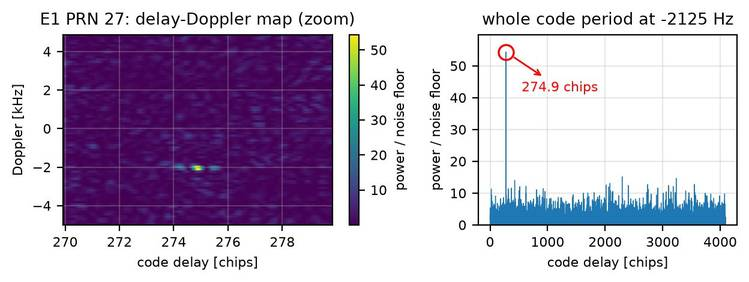
\includegraphics[width=1.0\linewidth]{gnss_sdr/x310_20261025T190000Z/galileo_acq_1B.jpg}
  \caption{Acquisition, E1: delay--Doppler search of PRN 27; one sharp peak (test statistic 76 vs threshold 52) at -2125~Hz and 274.9~chips.}
\end{figure}

\begin{figure}[H]
  \centering
  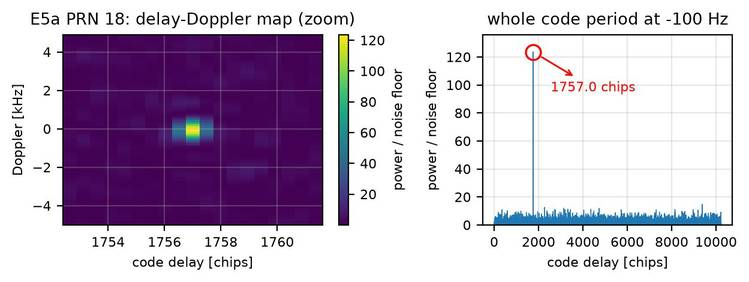
\includegraphics[width=1.0\linewidth]{gnss_sdr/x310_20261025T190000Z/galileo_acq_5X.jpg}
  \caption{Acquisition, E5a: delay--Doppler search of PRN 18; one sharp peak (test statistic 171 vs threshold 49) at -1556~Hz and 1757.0~chips.}
\end{figure}

\begin{table}[H]
  \centering
  \footnotesize
  \resizebox{\ifdim\width>\linewidth\linewidth\else\width\fi}{!}{%
  \begin{tabular}{lrrrr}
    \hline
    \textbf{Band} & \textbf{Attempts} & \textbf{Detections} & \textbf{Detected PRNs} & \textbf{Best statistic / threshold\footnotemark} \\
    \hline
    E1 & 4 & 1 & 27 & 1.5 \\
    E5a & 1 & 1 & 18 & 3.5 \\
    \hline
  \end{tabular}}
  \caption{Acquisition: search attempts of the dumped channel. Attempts on satellites that are not in view (or do not broadcast that signal, e.g. older GPS satellites on L5/L2C) are rejected below the threshold.}
\end{table}

\footnotetext{Margin of the band's strongest detection: the largest acquisition test statistic among the detected attempts (the correlation peak of the delay--Doppler grid, normalised by the power of the input samples searched, i.e. the noise power, since GNSS signals are below the noise) divided by the detection threshold, which GNSS-SDR derives from the configured probability of false alarm. A value of 1 is right at the detection limit; e.g. 2.5 means the peak cleared the threshold 2.5 times over.}

\subsubsection{Tracking}


\begin{figure}[H]
  \centering
  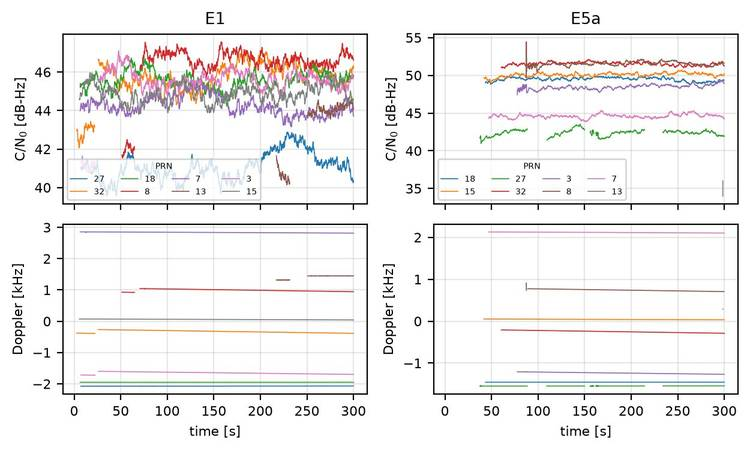
\includegraphics[width=1.0\linewidth]{gnss_sdr/x310_20261025T190000Z/galileo_tracking.jpg}
  \caption{Tracking: carrier-to-noise density ratio and carrier Doppler per satellite, while phase-locked (smooth Doppler curves = loops following the real satellite motion).}
\end{figure}

\begin{figure}[H]
  \centering
  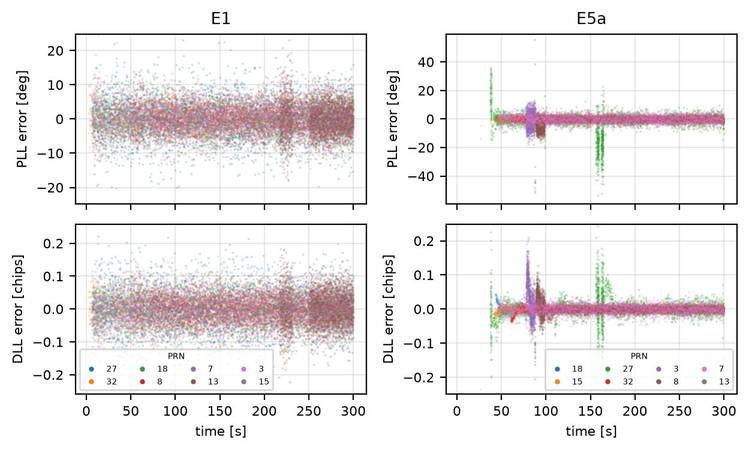
\includegraphics[width=1.0\linewidth]{gnss_sdr/x310_20261025T190000Z/galileo_tracking_errors.jpg}
  \caption{Tracking: loop errors per satellite while phase-locked, i.e. the discriminator outputs that the loops drive to zero: PLL carrier-phase error (degrees) and DLL code-delay error (chips) of every correlation. Noise centred on zero = clean tracking; its spread grows as C/N$_0$ drops, and jumps would mark cycle slips or a loop losing lock.}
\end{figure}

\begin{figure}[H]
  \centering
  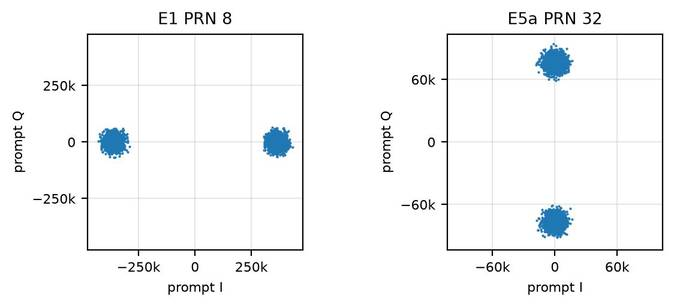
\includegraphics[width=1.0\linewidth]{gnss_sdr/x310_20261025T190000Z/galileo_tracking_iq.jpg}
  \caption{Tracking: prompt correlator outputs of the strongest satellite per band. Two tight clusters on one axis (the $\pm1$ data bits; GNSS-SDR's L5 tracking puts the data component on the Q axis), or, for the dataless pilots tracked for Galileo (E1-C, E5a-Q), the $\pm1$ chips of their secondary code, mean the PLL is phase-locked; a ring would mean it is not. \texttt{Prompt\_I}/\texttt{Prompt\_Q} are 32-bit floats (sums of the samples over one integration period, in file units): they never clip, only overflowing beyond $\pm 3.4\times10^{38}$, far above the $N\cdot\text{full scale}\cdot\sqrt{2}$ a sum of $N$ samples can reach.}
\end{figure}

\begin{table}[H]
  \centering
  \footnotesize
  \resizebox{\ifdim\width>\linewidth\linewidth\else\width\fi}{!}{%
  \begin{tabular}{lrrrrrrrr}
    \hline
    \textbf{Band} & \textbf{Ch.} & \textbf{PRN} & \textbf{Median C/N$_0$ [dB-Hz]} & \textbf{Phase-locked [\%]} & \textbf{Losses of lock} & \textbf{Tracked [s]} & \textbf{PLL error std [deg]} & \textbf{DLL error std [chips]} \\
    \hline
    E1 & 0 & 27 & 41.0 & 98 & 0 & 299 & 6.6 & 0.070 \\
    E1 & 1 & 32 & 45.8 & 98 & 1 & 299 & 3.7 & 0.040 \\
    E1 & 2 & 18 & 45.6 & 98 & 0 & 299 & 4.0 & 0.042 \\
    E1 & 3 & 8 & 46.5 & 82 & 3 & 298 & 3.8 & 0.039 \\
    E1 & 4 & 7 & 44.2 & 98 & 0 & 298 & 4.3 & 0.046 \\
    E1 & 5 & 13 & 43.8 & 21 & 12 & 300 & 4.8 & 0.052 \\
    E1 & 6 & 3 & 45.6 & 97 & 1 & 298 & 4.2 & 0.043 \\
    E1 & 7 & 15 & 44.9 & 98 & 0 & 300 & 3.9 & 0.042 \\
    E5a & 8 & 18 & 49.5 & 53 & 0 & 276 & 1.6 & 0.008 \\
    E5a & 9 & 15 & 50.1 & 53 & 0 & 274 & 1.6 & 0.012 \\
    E5a & 10 & 27 & 42.4 & 25 & 3 & 269 & 10.7 & 0.043 \\
    E5a & 11 & 32 & 51.4 & 51 & 0 & 256 & 1.3 & 0.007 \\
    E5a & 12 & 3 & 29.7 & 38 & 2 & 256 & 4.1 & 0.041 \\
    E5a & 13 & 8 & 51.4 & 93 & 0 & 213 & 6.2 & 0.026 \\
    E5a & 14 & 7 & 44.6 & 52 & 0 & 274 & 2.8 & 0.016 \\
    E5a & 15 & 13 & 29.0 & 0 & 2 & 34 & 28.5 & 0.177 \\
    \hline
  \end{tabular}}
  \caption{Tracking: per channel and satellite (phase-locked: carrier lock test $> 0.8$; loop error standard deviations while phase-locked).}
\end{table}

\subsubsection{Telemetry decoder}


\begin{figure}[H]
  \centering
  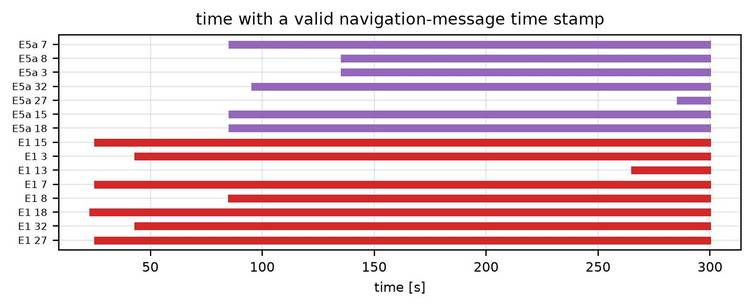
\includegraphics[width=1.0\linewidth]{gnss_sdr/x310_20261025T190000Z/galileo_telemetry.jpg}
  \caption{Telemetry decoder: per band and satellite, when the decoder delivered a valid transmit time (the first one comes after the first complete frame/message).}
\end{figure}

\begin{table}[H]
  \centering
  \footnotesize
  \resizebox{\ifdim\width>\linewidth\linewidth\else\width\fi}{!}{%
  \begin{tabular}{lrrrrr}
    \hline
    \textbf{Band} & \textbf{PRN} & \textbf{Messages decoded} & \textbf{Ephemeris} & \textbf{First valid at [s]} & \textbf{TOW [s]} \\
    \hline
    E1 & 3 & 25 & yes & 43.1 & 68468.0 \\
    E1 & 7 & 26 & yes & 25.1 & 68450.0 \\
    E1 & 8 & 21 & yes & 85.1 & 68510.0 \\
    E1 & 13 & 3 & yes & 265.1 & 68690.0 \\
    E1 & 15 & 26 & yes & 25.1 & 68450.0 \\
    E1 & 18 & 27 & yes & 23.1 & 68448.0 \\
    E1 & 27 & 26 & yes & 25.1 & 68450.0 \\
    E1 & 32 & 25 & yes & 43.1 & 68468.0 \\
    E5a & 3 & 9 & yes & 135.3 & 68560.3 \\
    E5a & 7 & 12 & yes & 85.3 & 68510.3 \\
    E5a & 8 & 9 & yes & 135.3 & 68560.3 \\
    E5a & 15 & 12 & yes & 85.3 & 68510.3 \\
    E5a & 18 & 11 & yes & 85.3 & 68510.3 \\
    E5a & 27 & -- & yes & 285.3 & 68710.3 \\
    E5a & 32 & 11 & yes & 95.3 & 68520.3 \\
    \hline
  \end{tabular}}
  \caption{Telemetry decoder: E1 I/NAV words, E5a F/NAV pages decoded, ephemeris obtained, and the first valid time of week.}
\end{table}

\subsubsection{Observables}
Pseudorange, carrier phase and Doppler of every channel at common receiver epochs.

\begin{figure}[H]
  \centering
  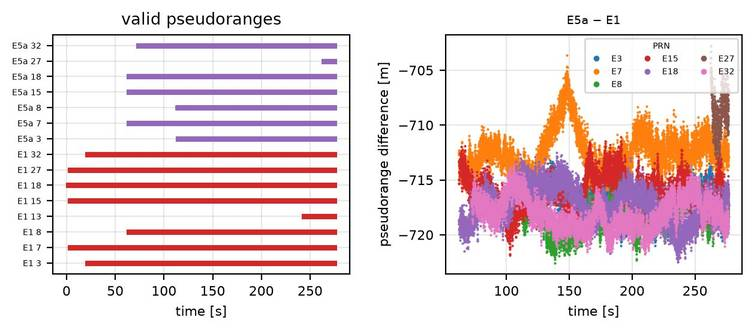
\includegraphics[width=1.0\linewidth]{gnss_sdr/x310_20261025T190000Z/galileo_observables.jpg}
  \caption{Observables: epochs with a valid pseudorange per band and satellite, and the difference between the two bands' pseudoranges of the same satellite (a constant receiver inter-band bias, the same for every satellite, plus the slowly varying ionospheric delay).}
\end{figure}

\begin{table}[H]
  \centering
  \footnotesize
  \resizebox{\ifdim\width>\linewidth\linewidth\else\width\fi}{!}{%
  \begin{tabular}{lrrrrrr}
    \hline
    \textbf{Difference} & \textbf{PRN} & \textbf{Common epochs} & \textbf{of run [\%]} & \textbf{Mean [m]} & \textbf{Std [m]} & \textbf{Drift [m/s]} \\
    \hline
    E5a $-$ E1 & 3 & 8206 & 55 & -717.05 & 1.31 & -0.0028 \\
    E5a $-$ E1 & 7 & 10398 & 69 & -712.39 & 1.87 & 0.0037 \\
    E5a $-$ E1 & 8 & 8207 & 55 & -718.19 & 1.48 & 0.0094 \\
    E5a $-$ E1 & 15 & 10422 & 70 & -716.17 & 1.51 & 0.0016 \\
    E5a $-$ E1 & 18 & 10398 & 69 & -717.25 & 1.64 & -0.0080 \\
    E5a $-$ E1 & 27 & 720 & 5 & -708.73 & 1.89 & 0.0081 \\
    E5a $-$ E1 & 32 & 9987 & 67 & -718.07 & 1.39 & -0.0022 \\
    \hline
  \end{tabular}}
  \caption{Observables: pseudorange difference between the two bands of each satellite at common epochs (similar means = shared receiver bias; std = code noise of both bands).}
\end{table}

\subsubsection{PVT}
Position from the pseudoranges and the decoded ephemeris, compared with the surveyed antenna position (-23.209433$^\circ$, -45.874875$^\circ$, 596.42~m).

\begin{figure}[H]
  \centering
  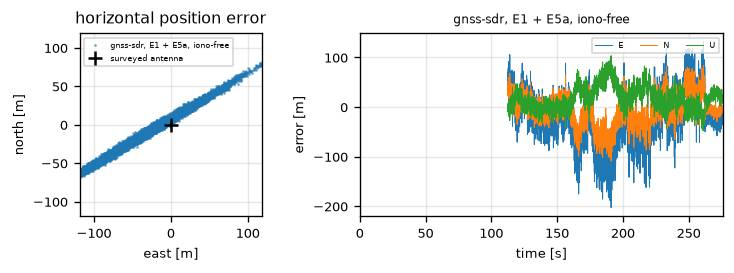
\includegraphics[width=1.0\linewidth]{gnss_sdr/x310_20261025T190000Z/galileo_pvt.jpg}
  \caption{PVT: position error of GNSS-SDR's own RTKLIB solution with respect to the surveyed antenna position.}
\end{figure}

\begin{table}[H]
  \centering
  \footnotesize
  \resizebox{\ifdim\width>\linewidth\linewidth\else\width\fi}{!}{%
  \begin{tabular}{l>{\centering\arraybackslash}p{4.2cm}}
    \hline
    \textbf{Solution} & \textbf{gnss-sdr, E1 + E5a, iono-free} \\
    \hline
    Solutions & 8535 \\
    Run with fix [\%] & 60 \\
    Mean E / N / U [m] & -25.3 / -7.1 / 17.7 \\
    Std E / N / U [m] & 51.5 / 30.6 / 23.4 \\
    RMS 2-D [m] & 65.4 \\
    RMS 3-D [m] & 71.7 \\
    95\% horiz. [m] & 133.9 \\
    \hline
  \end{tabular}}
  \caption{PVT: position error statistics with respect to the surveyed antenna (mean = accuracy, std = precision; \% of the run's seconds with a position; GNSS-SDR outputs several solutions per second).}
\end{table}




\subsection{Second record}
\begin{table}[H]
  \centering
  \begin{tabular}{|l|l|l|}
    \hline
    \textbf{Parameter} & \textbf{Channel 0} & \textbf{Channel 1} \\
    \hline
    Start time & \multicolumn{2}{>{\centering\arraybackslash}p{7cm}|}{2026-10-25 19:52:09 UTC} \\
    \hline
    Frequency & 1575.420 MHz (L1) & 1227.600 MHz (L2) \\
    \hline
    Duration & 300.0 s & 300.0 s \\
    \hline
    Sample rate & 4.000 MS/s & 4.000 MS/s \\
    \hline
    Sample type & \multicolumn{2}{>{\centering\arraybackslash}p{7cm}|}{signed complex 16-bit samples (I+Q), little-endian, as received from the X310 (sc16)} \\
    \hline
    Gain & 25.0 dB & 25.0 dB \\
    \hline
    Antenna & RX1 & RX2 \\
    \hline
    File size & 4800.0 MB & 4800.0 MB \\
    \hline
    Samples written & 1,200,000,000 & 1,200,000,000 \\
    \hline
    Lost samples & 0 & 0 \\
    \hline
    Clock source & \multicolumn{2}{>{\centering\arraybackslash}p{7cm}|}{external} \\
    \hline
    Time source & \multicolumn{2}{>{\centering\arraybackslash}p{7cm}|}{internal} \\
    \hline
    Motherboard & \multicolumn{2}{>{\centering\arraybackslash}p{7cm}|}{USRP X310} \\
    \hline
    Daughterboard & TwinRX RX0 & TwinRX RX1 \\
    \hline
    Recorder & \multicolumn{2}{>{\centering\arraybackslash}p{7cm}|}{UHD Python API} \\
    \hline
    GNSS-SDR configuration & \multicolumn{2}{>{\centering\arraybackslash}p{7cm}|}{\texttt{l1ca16bits4msps\_l2c16bits4msps.conf}} \\
    \hline
  \end{tabular}
  \caption{Metadata for recording \texttt{x310\_20261025T195201Z}, captured starting 2026-10-25T19:52:09.046382Z.}
\end{table}

\subsubsection{Signal source}
Raw I/Q samples of each channel analysed within the window [10, 10.5]~s after the start recording instant.

\begin{figure}[H]
  \centering
  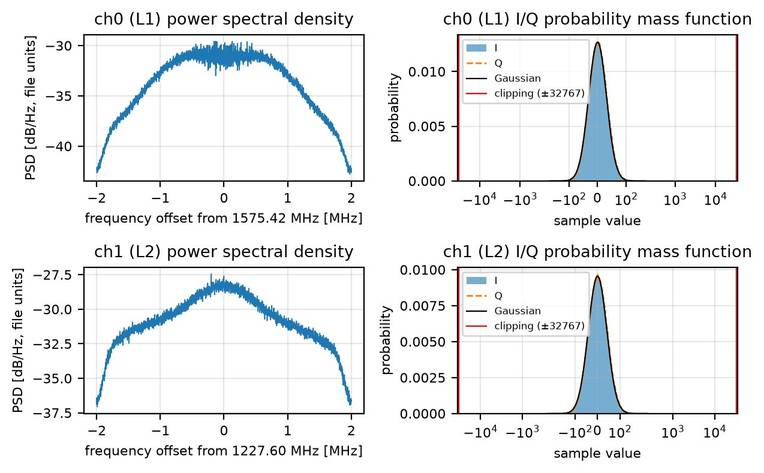
\includegraphics[width=1.0\linewidth]{gnss_sdr/x310_20261025T195201Z/source.jpg}
  \caption{Signal source: power spectral density (the receiver passband over a flat thermal-noise floor; GNSS signals are below the noise, so only interference would stand out) and probability mass functions of the integer I/Q sample values (Gaussian noise, centred, not clipped).}
\end{figure}

\begin{table}[H]
  \centering
  \footnotesize
  \resizebox{\ifdim\width>\linewidth\linewidth\else\width\fi}{!}{%
  \begin{tabular}{l>{\centering\arraybackslash}p{4.2cm}>{\centering\arraybackslash}p{4.2cm}}
    \hline
    \textbf{Channel} & \textbf{ch0} & \textbf{ch1} \\
    \hline
    Frequency [MHz] & 1575.42 & 1227.60 \\
    Rate [MS/s] & 4 & 4 \\
    Format & ci16\_le & ci16\_le \\
    Bytes per complex sample & 4 (2 for I, 2 for Q) & 4 (2 for I, 2 for Q) \\
    Full scale & $\pm$32767 & $\pm$32767 \\
    Gain [dB] & 25 & 25 \\
    Std I / Q & 31.5 / 31.5 & 41.8 / 41.9 \\
    Mean I / Q & -0.03 / 0.01 & 0.20 / -0.00 \\
    Min / max I & -150 / 162 & -197 / 207 \\
    Min / max Q & -149 / 177 & -208 / 205 \\
    Headroom\footnotemark & 1040.8 & 783.7 \\
    Clipped [\%] & 0.000 & 0.000 \\
    Lost samples & 0 & 0 \\
    \hline
  \end{tabular}}
  \caption{Signal source: sample statistics per channel (headroom: how many standard deviations of the noise fit before clipping).}
\end{table}

\footnotetext{Headroom $= A/\sigma$, where $A$ is the full scale of the sample format (127 for 8-bit, 32767 for 16-bit) and $\sigma$ the standard deviation of the I and Q samples together (both in file units, over the analysed window). For Gaussian noise, the fraction of clipped values is $2Q(A/\sigma)$, with $Q$ the Gaussian tail function: e.g. 0.003\,\% at $4.2\sigma$.}

\subsubsection{Signal conditioner}


\begin{table}[H]
  \centering
  \footnotesize
  \resizebox{\ifdim\width>\linewidth\linewidth\else\width\fi}{!}{%
  \begin{tabular}{l>{\centering\arraybackslash}p{4.2cm}>{\centering\arraybackslash}p{4.2cm}}
    \hline
    \textbf{Channel} & \textbf{ch0 (L1 C/A, E1)} & \textbf{ch1 (L2C)} \\
    \hline
    File format & ci16\_le & ci16\_le \\
    Source item type & ishort & ishort \\
    Data type adapter & Ishort\_To\_Complex & Ishort\_To\_Complex \\
    Input filter & Pass\_Through & Pass\_Through \\
    Resampling & Pass\_Through & Pass\_Through \\
    Rate [MS/s] & 4 $\to$ 4 & 4 $\to$ 4 \\
    \hline
  \end{tabular}}
  \caption{Signal conditioner: recorded format and rate to gnss-sdr's internal \texttt{gr\_complex} stream; both bands are read in lockstep by one \texttt{Multichannel\_File\_Signal\_Source}.}
\end{table}

\subsubsection{Acquisition}
Two-dimensional search over code delay and Doppler (one channel per band dumped; the others behave alike).

\begin{figure}[H]
  \centering
  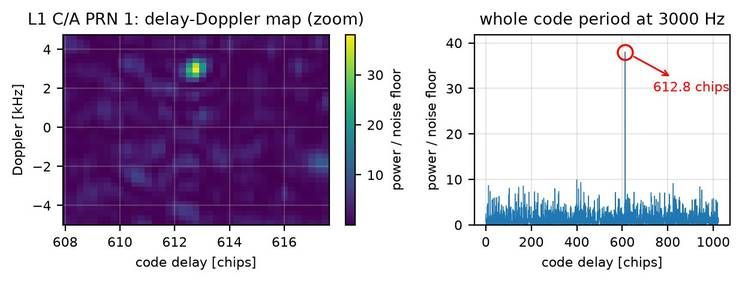
\includegraphics[width=1.0\linewidth]{gnss_sdr/x310_20261025T195201Z/acq_1C.jpg}
  \caption{Acquisition, L1 C/A: delay--Doppler search of PRN 1; one sharp peak (test statistic 51 vs threshold 44) at 3000~Hz and 612.8~chips.}
\end{figure}

\begin{figure}[H]
  \centering
  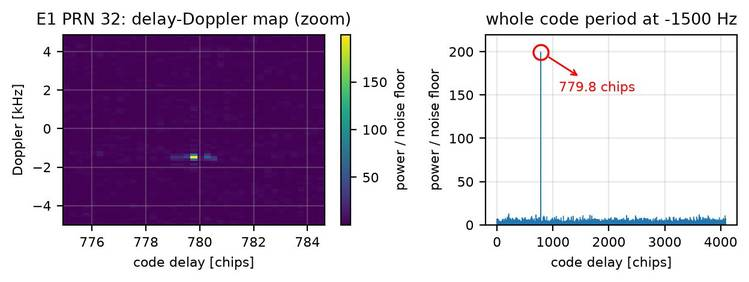
\includegraphics[width=1.0\linewidth]{gnss_sdr/x310_20261025T195201Z/acq_1B.jpg}
  \caption{Acquisition, E1: delay--Doppler search of PRN 32; one sharp peak (test statistic 277 vs threshold 48) at -1500~Hz and 779.8~chips.}
\end{figure}

\begin{table}[H]
  \centering
  \footnotesize
  \resizebox{\ifdim\width>\linewidth\linewidth\else\width\fi}{!}{%
  \begin{tabular}{lrrrr}
    \hline
    \textbf{Band} & \textbf{Attempts} & \textbf{Detections} & \textbf{Detected PRNs} & \textbf{Best statistic / threshold\footnotemark} \\
    \hline
    L1 C/A & 1 & 1 & 1 & 1.2 \\
    L2C & \multicolumn{4}{l}{not dumped (search grid too large); acquired satellites: see the tracking table} \\
    E1 & 5 & 1 & 32 & 5.7 \\
    \hline
  \end{tabular}}
  \caption{Acquisition: search attempts of the dumped channel. Attempts on satellites that are not in view (or do not broadcast that signal, e.g. older GPS satellites on L5/L2C) are rejected below the threshold.}
\end{table}

\footnotetext{Margin of the band's strongest detection: the largest acquisition test statistic among the detected attempts (the correlation peak of the delay--Doppler grid, normalised by the power of the input samples searched, i.e. the noise power, since GNSS signals are below the noise) divided by the detection threshold, which GNSS-SDR derives from the configured probability of false alarm. A value of 1 is right at the detection limit; e.g. 2.5 means the peak cleared the threshold 2.5 times over.}

\subsubsection{Tracking}


\begin{figure}[H]
  \centering
  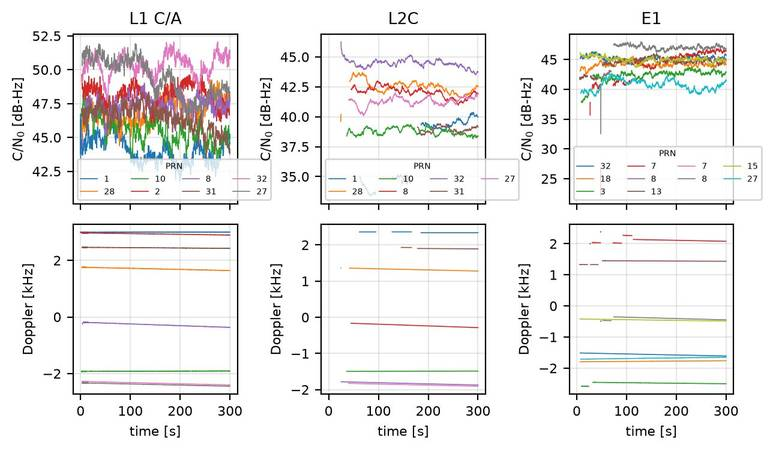
\includegraphics[width=1.0\linewidth]{gnss_sdr/x310_20261025T195201Z/tracking.jpg}
  \caption{Tracking: carrier-to-noise density ratio and carrier Doppler per satellite, while phase-locked (smooth Doppler curves = loops following the real satellite motion).}
\end{figure}

\begin{figure}[H]
  \centering
  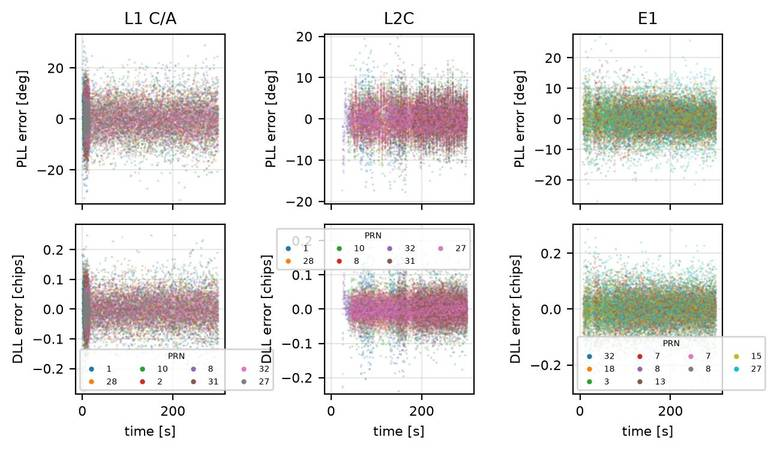
\includegraphics[width=1.0\linewidth]{gnss_sdr/x310_20261025T195201Z/tracking_errors.jpg}
  \caption{Tracking: loop errors per satellite while phase-locked, i.e. the discriminator outputs that the loops drive to zero: PLL carrier-phase error (degrees) and DLL code-delay error (chips) of every correlation. Noise centred on zero = clean tracking; its spread grows as C/N$_0$ drops, and jumps would mark cycle slips or a loop losing lock.}
\end{figure}

\begin{figure}[H]
  \centering
  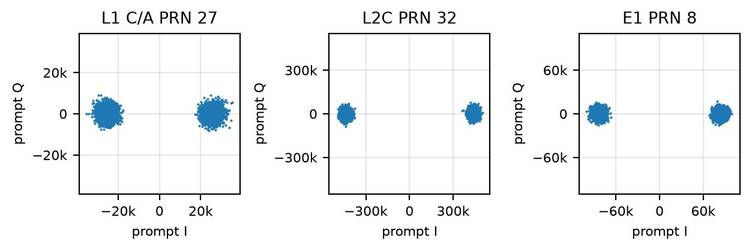
\includegraphics[width=1.0\linewidth]{gnss_sdr/x310_20261025T195201Z/tracking_iq.jpg}
  \caption{Tracking: prompt correlator outputs of the strongest satellite per band. Two tight clusters on one axis (the $\pm1$ data bits; GNSS-SDR's L5 tracking puts the data component on the Q axis), or, for the dataless pilots tracked for Galileo (E1-C, E5a-Q), the $\pm1$ chips of their secondary code, mean the PLL is phase-locked; a ring would mean it is not. \texttt{Prompt\_I}/\texttt{Prompt\_Q} are 32-bit floats (sums of the samples over one integration period, in file units): they never clip, only overflowing beyond $\pm 3.4\times10^{38}$, far above the $N\cdot\text{full scale}\cdot\sqrt{2}$ a sum of $N$ samples can reach.}
\end{figure}

\begin{table}[H]
  \centering
  \footnotesize
  \resizebox{\ifdim\width>\linewidth\linewidth\else\width\fi}{!}{%
  \begin{tabular}{lrrrrrrrr}
    \hline
    \textbf{Band} & \textbf{Ch.} & \textbf{PRN} & \textbf{Median C/N$_0$ [dB-Hz]} & \textbf{Phase-locked [\%]} & \textbf{Losses of lock} & \textbf{Tracked [s]} & \textbf{PLL error std [deg]} & \textbf{DLL error std [chips]} \\
    \hline
    L1 C/A & 0 & 1 & 44.3 & 100 & 0 & 300 & 8.9 & 0.071 \\
    L1 C/A & 1 & 28 & 46.4 & 97 & 0 & 298 & 6.6 & 0.052 \\
    L1 C/A & 2 & 10 & 46.1 & 94 & 0 & 300 & 7.2 & 0.055 \\
    L1 C/A & 3 & 2 & 48.4 & 97 & 0 & 298 & 5.7 & 0.042 \\
    L1 C/A & 4 & 8 & 47.2 & 95 & 0 & 296 & 6.4 & 0.050 \\
    L1 C/A & 5 & 31 & 46.6 & 95 & 0 & 298 & 6.9 & 0.052 \\
    L1 C/A & 6 & 32 & 50.2 & 95 & 0 & 298 & 4.4 & 0.033 \\
    L1 C/A & 7 & 27 & 50.7 & 95 & 0 & 298 & 4.5 & 0.034 \\
    L2C & 8 & 1 & 36.7 & 68 & 2 & 276 & 5.0 & 0.056 \\
    L2C & 9 & 28 & 42.5 & 94 & 0 & 276 & 3.8 & 0.030 \\
    L2C & 10 & 10 & 38.7 & 96 & 0 & 276 & 4.3 & 0.043 \\
    L2C & 12 & 8 & 42.1 & 93 & 0 & 276 & 3.3 & 0.029 \\
    L2C & 13 & 32 & 44.5 & 100 & 0 & 276 & 3.0 & 0.025 \\
    L2C & 14 & 31 & 37.3 & 52 & 2 & 276 & 4.4 & 0.044 \\
    L2C & 15 & 27 & 41.3 & 95 & 0 & 275 & 3.5 & 0.033 \\
    E1 & 16 & 32 & 45.2 & 99 & 0 & 297 & 3.8 & 0.045 \\
    E1 & 17 & 18 & 44.1 & 98 & 0 & 299 & 4.7 & 0.052 \\
    E1 & 18 & 3 & 42.5 & 96 & 1 & 294 & 5.7 & 0.065 \\
    E1 & 19 & 7 & 44.6 & 87 & 5 & 273 & 5.2 & 0.052 \\
    E1 & 19 & 8 & 45.3 & 0 & 5 & 21 & -- & -- \\
    E1 & 20 & 13 & 44.7 & 94 & 2 & 296 & 4.1 & 0.046 \\
    E1 & 21 & 7 & 44.0 & 0 & 3 & 21 & -- & -- \\
    E1 & 21 & 8 & 46.9 & 89 & 3 & 273 & 4.2 & 0.040 \\
    E1 & 22 & 15 & 45.0 & 98 & 0 & 299 & 3.9 & 0.046 \\
    E1 & 23 & 27 & 40.7 & 98 & 0 & 298 & 6.9 & 0.079 \\
    \hline
  \end{tabular}}
  \caption{Tracking: per channel and satellite (phase-locked: carrier lock test $> 0.8$; loop error standard deviations while phase-locked).}
\end{table}

\subsubsection{Telemetry decoder}


\begin{figure}[H]
  \centering
  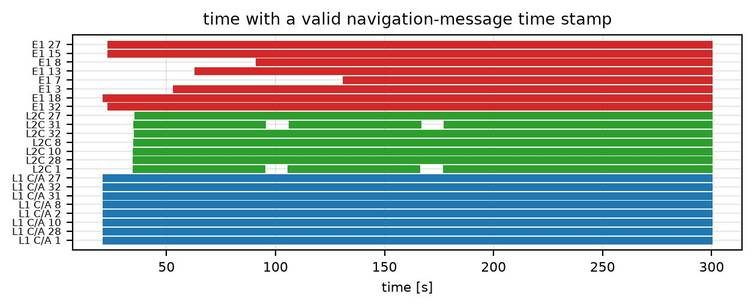
\includegraphics[width=1.0\linewidth]{gnss_sdr/x310_20261025T195201Z/telemetry.jpg}
  \caption{Telemetry decoder: per band and satellite, when the decoder delivered a valid transmit time (the first one comes after the first complete frame/message).}
\end{figure}

\begin{table}[H]
  \centering
  \footnotesize
  \resizebox{\ifdim\width>\linewidth\linewidth\else\width\fi}{!}{%
  \begin{tabular}{lrrrrr}
    \hline
    \textbf{Band} & \textbf{PRN} & \textbf{Messages decoded} & \textbf{Ephemeris} & \textbf{First valid at [s]} & \textbf{TOW [s]} \\
    \hline
    E1 & 3 & 23 & yes & 53.1 & 71600.0 \\
    E1 & 7 & 16 & yes & 131.1 & 71678.0 \\
    E1 & 8 & 21 & yes & 91.1 & 71638.0 \\
    E1 & 13 & 22 & yes & 63.1 & 71610.0 \\
    E1 & 15 & 26 & yes & 23.1 & 71570.0 \\
    E1 & 18 & 26 & yes & 21.1 & 71568.0 \\
    E1 & 27 & 27 & yes & 23.1 & 71570.0 \\
    E1 & 32 & 27 & yes & 23.1 & 71570.0 \\
    L1 C/A & 1 & 46 & yes & 21.0 & 71568.0 \\
    L1 C/A & 2 & 33 & yes & 21.0 & 71568.0 \\
    L1 C/A & 8 & 36 & yes & 21.0 & 71568.0 \\
    L1 C/A & 10 & 47 & yes & 21.0 & 71568.0 \\
    L1 C/A & 27 & 39 & yes & 21.0 & 71568.0 \\
    L1 C/A & 28 & 46 & yes & 21.0 & 71568.0 \\
    L1 C/A & 31 & 47 & yes & 21.0 & 71568.0 \\
    L1 C/A & 32 & 44 & yes & 21.0 & 71568.0 \\
    L2C & 1 & 7 & yes & 34.8 & 0.0 \\
    L2C & 8 & 13 & yes & 35.0 & 0.0 \\
    L2C & 10 & 13 & yes & 34.9 & 0.0 \\
    L2C & 27 & 13 & yes & 35.6 & 0.0 \\
    L2C & 28 & 16 & yes & 34.8 & 0.0 \\
    L2C & 31 & 6 & yes & 35.2 & 0.0 \\
    L2C & 32 & 13 & yes & 35.4 & 0.0 \\
    \hline
  \end{tabular}}
  \caption{Telemetry decoder: L1 C/A LNAV subframes, L2C CNAV messages, E1 I/NAV words decoded, ephemeris obtained, and the first valid time of week.}
\end{table}

\subsubsection{Observables}
Pseudorange, carrier phase and Doppler of every channel at common receiver epochs.

\begin{figure}[H]
  \centering
  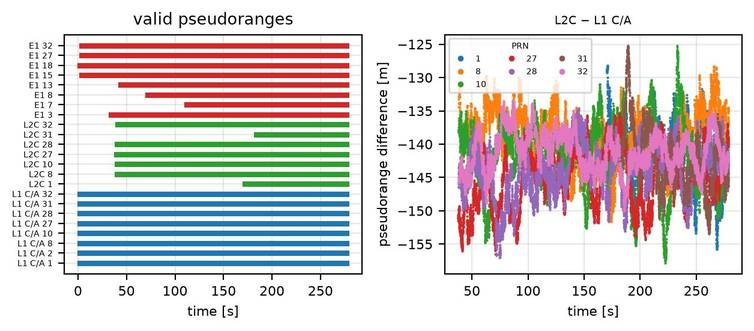
\includegraphics[width=1.0\linewidth]{gnss_sdr/x310_20261025T195201Z/observables.jpg}
  \caption{Observables: epochs with a valid pseudorange per band and satellite, and the difference between the two bands' pseudoranges of the same satellite (a constant receiver inter-band bias, the same for every satellite, plus the slowly varying ionospheric delay).}
\end{figure}

\begin{table}[H]
  \centering
  \footnotesize
  \resizebox{\ifdim\width>\linewidth\linewidth\else\width\fi}{!}{%
  \begin{tabular}{lrrrrrr}
    \hline
    \textbf{Difference} & \textbf{PRN} & \textbf{Common epochs} & \textbf{of run [\%]} & \textbf{Mean [m]} & \textbf{Std [m]} & \textbf{Drift [m/s]} \\
    \hline
    L2C $-$ L1 C/A & 1 & 5420 & 36 & -141.16 & 4.36 & -0.0391 \\
    L2C $-$ L1 C/A & 8 & 12020 & 80 & -138.93 & 3.76 & -0.0024 \\
    L2C $-$ L1 C/A & 10 & 12026 & 80 & -141.77 & 4.86 & -0.0059 \\
    L2C $-$ L1 C/A & 27 & 12052 & 80 & -145.24 & 4.16 & 0.0175 \\
    L2C $-$ L1 C/A & 28 & 12030 & 80 & -143.94 & 3.79 & 0.0182 \\
    L2C $-$ L1 C/A & 31 & 4826 & 32 & -142.15 & 4.64 & -0.0814 \\
    L2C $-$ L1 C/A & 32 & 12000 & 80 & -141.08 & 2.83 & -0.0038 \\
    \hline
  \end{tabular}}
  \caption{Observables: pseudorange difference between the two bands of each satellite at common epochs (similar means = shared receiver bias; std = code noise of both bands).}
\end{table}

\subsubsection{PVT}
Position from the pseudoranges and the decoded ephemeris, compared with the surveyed antenna position (-23.209433$^\circ$, -45.874875$^\circ$, 596.42~m).

\begin{figure}[H]
  \centering
  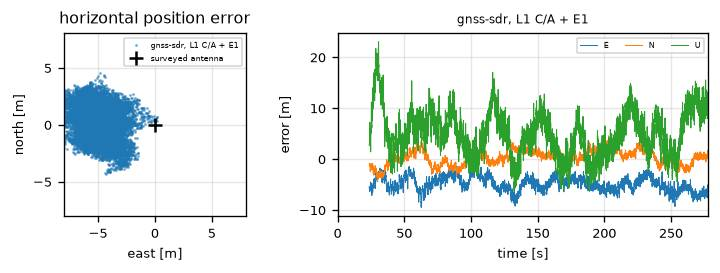
\includegraphics[width=1.0\linewidth]{gnss_sdr/x310_20261025T195201Z/pvt.jpg}
  \caption{PVT: position error of GNSS-SDR's own RTKLIB solution with respect to the surveyed antenna position (single frequency, broadcast ionosphere model).}
\end{figure}

\begin{table}[H]
  \centering
  \footnotesize
  \resizebox{\ifdim\width>\linewidth\linewidth\else\width\fi}{!}{%
  \begin{tabular}{l>{\centering\arraybackslash}p{4.2cm}}
    \hline
    \textbf{Solution} & \textbf{gnss-sdr, L1 C/A + E1} \\
    \hline
    Solutions & 13243 \\
    Run with fix [\%] & 92 \\
    Mean E / N / U [m] & -4.9 / 0.3 / 5.1 \\
    Std E / N / U [m] & 1.4 / 1.5 / 4.5 \\
    RMS 2-D [m] & 5.3 \\
    RMS 3-D [m] & 8.6 \\
    95\% horiz. [m] & 7.3 \\
    \hline
  \end{tabular}}
  \caption{PVT: position error statistics with respect to the surveyed antenna (mean = accuracy, std = precision; \% of the run's seconds with a position; GNSS-SDR outputs several solutions per second).}
\end{table}




\section{Records on 26/10/2026}

\subsection{First record}
\begin{table}[H]
  \centering
  \begin{tabular}{|l|l|l|}
    \hline
    \textbf{Parameter} & \textbf{Channel 0} & \textbf{Channel 1} \\
    \hline
    Start time & \multicolumn{2}{>{\centering\arraybackslash}p{7cm}|}{2026-10-26 19:00:08 UTC} \\
    \hline
    Frequency & 1575.420 MHz (L1) & 1176.450 MHz (L5) \\
    \hline
    Duration & 300.0 s & 300.0 s \\
    \hline
    Sample rate & 4.000 MS/s & 20.000 MS/s \\
    \hline
    Sample type & \multicolumn{2}{>{\centering\arraybackslash}p{7cm}|}{signed complex 8-bit samples (I+Q), converted on the host from the X310's sc16} \\
    \hline
    Gain & 25.0 dB & 25.0 dB \\
    \hline
    Antenna & RX1 & RX2 \\
    \hline
    File size & 2400.0 MB & 12000.0 MB \\
    \hline
    Samples written & 1,200,000,000 & 6,000,000,000 \\
    \hline
    Lost samples & 0 & 3287000 \\
    \hline
    Clock source & \multicolumn{2}{>{\centering\arraybackslash}p{7cm}|}{external} \\
    \hline
    Time source & \multicolumn{2}{>{\centering\arraybackslash}p{7cm}|}{internal} \\
    \hline
    Motherboard & \multicolumn{2}{>{\centering\arraybackslash}p{7cm}|}{USRP X310} \\
    \hline
    Daughterboard & TwinRX RX0 & TwinRX RX1 \\
    \hline
    Recorder & \multicolumn{2}{>{\centering\arraybackslash}p{7cm}|}{UHD Python API} \\
    \hline
    GNSS-SDR configuration & \multicolumn{2}{>{\centering\arraybackslash}p{7cm}|}{\texttt{l1ca8bits4msps\_l5\_8bits20msps.conf}, \texttt{e1\_8bits4msps\_e5a\_8bits20msps.conf}} \\
    \hline
  \end{tabular}
  \caption{Metadata for recording \texttt{x310\_20261026T190001Z}, captured starting 2026-10-26T19:00:08.297684Z.}
\end{table}

\subsubsection{Signal source}
Raw I/Q samples of each channel analysed within the window [10, 10.5]~s after the start recording instant.

\begin{figure}[H]
  \centering
  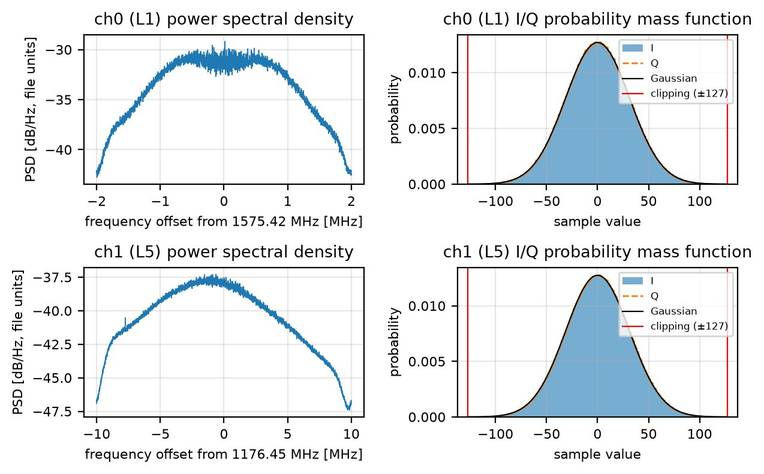
\includegraphics[width=1.0\linewidth]{gnss_sdr/x310_20261026T190001Z/source.jpg}
  \caption{Signal source: power spectral density (the receiver passband over a flat thermal-noise floor; GNSS signals are below the noise, so only interference would stand out) and probability mass functions of the integer I/Q sample values (Gaussian noise, centred, not clipped).}
\end{figure}

\begin{table}[H]
  \centering
  \footnotesize
  \resizebox{\ifdim\width>\linewidth\linewidth\else\width\fi}{!}{%
  \begin{tabular}{l>{\centering\arraybackslash}p{4.2cm}>{\centering\arraybackslash}p{4.2cm}}
    \hline
    \textbf{Channel} & \textbf{ch0} & \textbf{ch1} \\
    \hline
    Frequency [MHz] & 1575.42 & 1176.45 \\
    Rate [MS/s] & 4 & 20 \\
    Format & ci8 & ci8 \\
    Bytes per complex sample & 2 (1 for I, 1 for Q) & 2 (1 for I, 1 for Q) \\
    Full scale & $\pm$127 & $\pm$127 \\
    Gain [dB] & 25 & 25 \\
    Std I / Q & 31.4 / 31.4 & 31.3 / 31.3 \\
    Mean I / Q & 0.02 / -0.15 & -0.03 / 0.04 \\
    Min / max I & -127 / 127 & -127 / 127 \\
    Min / max Q & -127 / 127 & -127 / 127 \\
    Headroom\footnotemark & 4.0 & 4.1 \\
    Clipped [\%] & 0.004 & 0.005 \\
    Lost samples & 0 & 3,287,000 \\
    \hline
  \end{tabular}}
  \caption{Signal source: sample statistics per channel (headroom: how many standard deviations of the noise fit before clipping).}
\end{table}

\footnotetext{Headroom $= A/\sigma$, where $A$ is the full scale of the sample format (127 for 8-bit, 32767 for 16-bit) and $\sigma$ the standard deviation of the I and Q samples together (both in file units, over the analysed window). For Gaussian noise, the fraction of clipped values is $2Q(A/\sigma)$, with $Q$ the Gaussian tail function: e.g. 0.003\,\% at $4.2\sigma$.}

\subsubsection{Signal conditioner}


\begin{table}[H]
  \centering
  \footnotesize
  \resizebox{\ifdim\width>\linewidth\linewidth\else\width\fi}{!}{%
  \begin{tabular}{l>{\centering\arraybackslash}p{4.2cm}>{\centering\arraybackslash}p{4.2cm}}
    \hline
    \textbf{Channel} & \textbf{ch0 (L1 C/A)} & \textbf{ch1 (L5)} \\
    \hline
    File format & ci8 & ci8 \\
    Source item type & ibyte & ibyte \\
    Data type adapter & Ibyte\_To\_Complex & Ibyte\_To\_Complex \\
    Input filter & Pass\_Through & Pass\_Through \\
    Resampling & $\times$5 zero-order hold, offline (\texttt{upsample\_iq.py}) & Pass\_Through \\
    Rate [MS/s] & 4 $\to$ 20 & 20 $\to$ 20 \\
    \hline
  \end{tabular}}
  \caption{Signal conditioner: recorded format and rate to gnss-sdr's internal \texttt{gr\_complex} stream; both bands are read in lockstep by one \texttt{Multichannel\_File\_Signal\_Source}.}
\end{table}

\subsubsection{Acquisition}
Two-dimensional search over code delay and Doppler (one channel per band dumped; the others behave alike).

\begin{figure}[H]
  \centering
  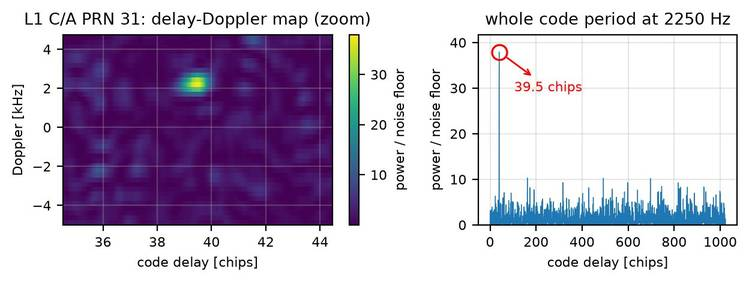
\includegraphics[width=1.0\linewidth]{gnss_sdr/x310_20261026T190001Z/acq_1C.jpg}
  \caption{Acquisition, L1 C/A: delay--Doppler search of PRN 31; one sharp peak (test statistic 51 vs threshold 47) at 2250~Hz and 39.5~chips.}
\end{figure}

\begin{figure}[H]
  \centering
  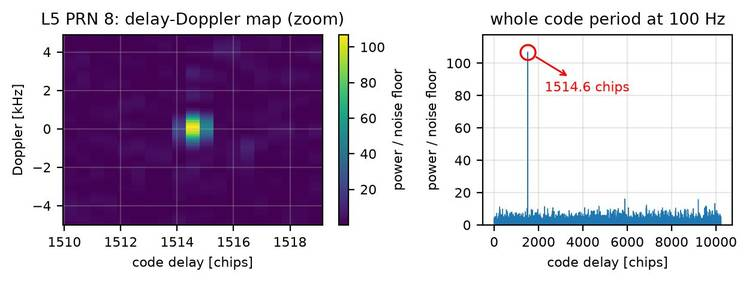
\includegraphics[width=1.0\linewidth]{gnss_sdr/x310_20261026T190001Z/acq_L5.jpg}
  \caption{Acquisition, L5: delay--Doppler search of PRN 8; one sharp peak (test statistic 148 vs threshold 49) at 1278~Hz and 1514.6~chips.}
\end{figure}

\begin{table}[H]
  \centering
  \footnotesize
  \resizebox{\ifdim\width>\linewidth\linewidth\else\width\fi}{!}{%
  \begin{tabular}{lrrrr}
    \hline
    \textbf{Band} & \textbf{Attempts} & \textbf{Detections} & \textbf{Detected PRNs} & \textbf{Best statistic / threshold\footnotemark} \\
    \hline
    L1 C/A & 3039 & 1 & 31 & 1.1 \\
    L5 & 1 & 1 & 8 & 3.0 \\
    \hline
  \end{tabular}}
  \caption{Acquisition: search attempts of the dumped channel. Attempts on satellites that are not in view (or do not broadcast that signal, e.g. older GPS satellites on L5/L2C) are rejected below the threshold.}
\end{table}

\footnotetext{Margin of the band's strongest detection: the largest acquisition test statistic among the detected attempts (the correlation peak of the delay--Doppler grid, normalised by the power of the input samples searched, i.e. the noise power, since GNSS signals are below the noise) divided by the detection threshold, which GNSS-SDR derives from the configured probability of false alarm. A value of 1 is right at the detection limit; e.g. 2.5 means the peak cleared the threshold 2.5 times over.}

\subsubsection{Tracking}


\begin{figure}[H]
  \centering
  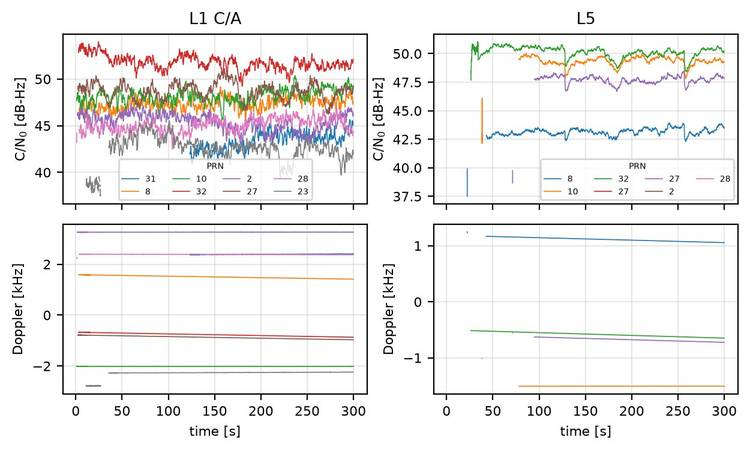
\includegraphics[width=1.0\linewidth]{gnss_sdr/x310_20261026T190001Z/tracking.jpg}
  \caption{Tracking: carrier-to-noise density ratio and carrier Doppler per satellite, while phase-locked (smooth Doppler curves = loops following the real satellite motion).}
\end{figure}

\begin{figure}[H]
  \centering
  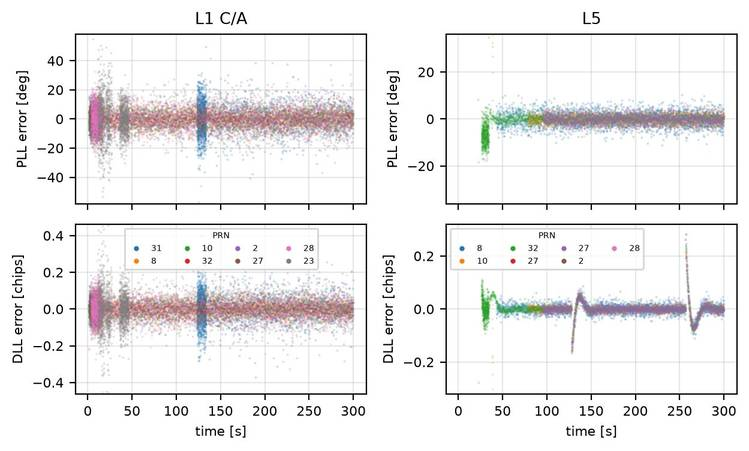
\includegraphics[width=1.0\linewidth]{gnss_sdr/x310_20261026T190001Z/tracking_errors.jpg}
  \caption{Tracking: loop errors per satellite while phase-locked, i.e. the discriminator outputs that the loops drive to zero: PLL carrier-phase error (degrees) and DLL code-delay error (chips) of every correlation. Noise centred on zero = clean tracking; its spread grows as C/N$_0$ drops, and jumps would mark cycle slips or a loop losing lock.}
\end{figure}

\begin{figure}[H]
  \centering
  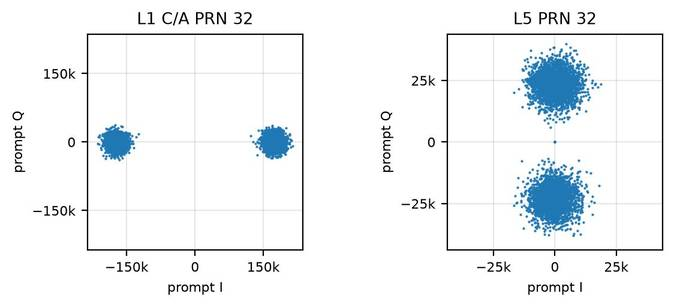
\includegraphics[width=1.0\linewidth]{gnss_sdr/x310_20261026T190001Z/tracking_iq.jpg}
  \caption{Tracking: prompt correlator outputs of the strongest satellite per band. Two tight clusters on one axis (the $\pm1$ data bits; GNSS-SDR's L5 tracking puts the data component on the Q axis), or, for the dataless pilots tracked for Galileo (E1-C, E5a-Q), the $\pm1$ chips of their secondary code, mean the PLL is phase-locked; a ring would mean it is not. \texttt{Prompt\_I}/\texttt{Prompt\_Q} are 32-bit floats (sums of the samples over one integration period, in file units): they never clip, only overflowing beyond $\pm 3.4\times10^{38}$, far above the $N\cdot\text{full scale}\cdot\sqrt{2}$ a sum of $N$ samples can reach.}
\end{figure}

\begin{table}[H]
  \centering
  \footnotesize
  \resizebox{\ifdim\width>\linewidth\linewidth\else\width\fi}{!}{%
  \begin{tabular}{lrrrrrrrr}
    \hline
    \textbf{Band} & \textbf{Ch.} & \textbf{PRN} & \textbf{Median C/N$_0$ [dB-Hz]} & \textbf{Phase-locked [\%]} & \textbf{Losses of lock} & \textbf{Tracked [s]} & \textbf{PLL error std [deg]} & \textbf{DLL error std [chips]} \\
    \hline
    L1 C/A & 0 & 31 & 42.5 & 88 & 0 & 179 & 10.5 & 0.079 \\
    L1 C/A & 1 & 8 & 47.2 & 95 & 0 & 298 & 6.3 & 0.047 \\
    L1 C/A & 2 & 10 & 48.0 & 96 & 0 & 300 & 5.7 & 0.041 \\
    L1 C/A & 3 & 32 & 52.6 & 95 & 0 & 299 & 3.5 & 0.025 \\
    L1 C/A & 4 & 2 & 46.0 & 98 & 0 & 299 & 7.4 & 0.055 \\
    L1 C/A & 5 & 27 & 49.0 & 95 & 0 & 299 & 5.1 & 0.037 \\
    L1 C/A & 6 & 28 & 44.9 & 90 & 0 & 299 & 8.4 & 0.060 \\
    L1 C/A & 7 & 23 & 42.0 & 77 & 1 & 287 & 13.4 & 0.097 \\
    L5 & 8 & 8 & 43.1 & 68 & 0 & 278 & 3.6 & 0.031 \\
    L5 & 9 & 10 & 48.1 & 34 & 2 & 278 & 2.9 & 0.029 \\
    L5 & 10 & 32 & 50.3 & 91 & 0 & 277 & 4.2 & 0.029 \\
    L5 & 12 & 27 & 28.9 & 0 & 2 & 32 & -- & -- \\
    L5 & 14 & 27 & 47.6 & 42 & 1 & 245 & 2.4 & 0.031 \\
    L5 & 15 & 2 & 28.7 & 0 & 2 & 16 & -- & -- \\
    L5 & 15 & 28 & 29.0 & 0 & 2 & 16 & -- & -- \\
    \hline
  \end{tabular}}
  \caption{Tracking: per channel and satellite (phase-locked: carrier lock test $> 0.8$; loop error standard deviations while phase-locked).}
\end{table}

\subsubsection{Telemetry decoder}


\begin{figure}[H]
  \centering
  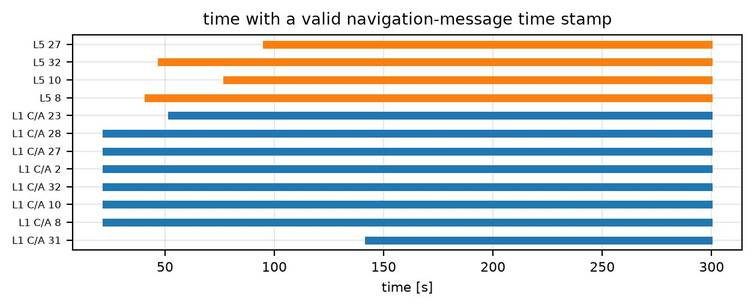
\includegraphics[width=1.0\linewidth]{gnss_sdr/x310_20261026T190001Z/telemetry.jpg}
  \caption{Telemetry decoder: per band and satellite, when the decoder delivered a valid transmit time (the first one comes after the first complete frame/message).}
\end{figure}

\begin{table}[H]
  \centering
  \footnotesize
  \resizebox{\ifdim\width>\linewidth\linewidth\else\width\fi}{!}{%
  \begin{tabular}{lrrrrr}
    \hline
    \textbf{Band} & \textbf{PRN} & \textbf{Messages decoded} & \textbf{Ephemeris} & \textbf{First valid at [s]} & \textbf{TOW [s]} \\
    \hline
    L1 C/A & 2 & 46 & yes & 21.8 & 154848.0 \\
    L1 C/A & 8 & 47 & yes & 21.8 & 154848.0 \\
    L1 C/A & 10 & 47 & yes & 21.8 & 154848.0 \\
    L1 C/A & 23 & 42 & yes & 51.8 & 154878.0 \\
    L1 C/A & 27 & 47 & yes & 21.8 & 154848.0 \\
    L1 C/A & 28 & 46 & yes & 21.8 & 154848.0 \\
    L1 C/A & 31 & 27 & yes & 141.8 & 154968.0 \\
    L1 C/A & 32 & 47 & yes & 21.8 & 154848.0 \\
    L5 & 8 & 27 & yes & 41.0 & 154867.3 \\
    L5 & 10 & 23 & yes & 76.9 & 154903.1 \\
    L5 & 27 & 21 & yes & 95.1 & 154921.4 \\
    L5 & 32 & 26 & yes & 46.9 & 154873.1 \\
    \hline
  \end{tabular}}
  \caption{Telemetry decoder: L1 C/A LNAV subframes, L5 CNAV messages decoded, ephemeris obtained, and the first valid time of week.}
\end{table}

\subsubsection{Observables}
Pseudorange, carrier phase and Doppler of every channel at common receiver epochs.

\begin{figure}[H]
  \centering
  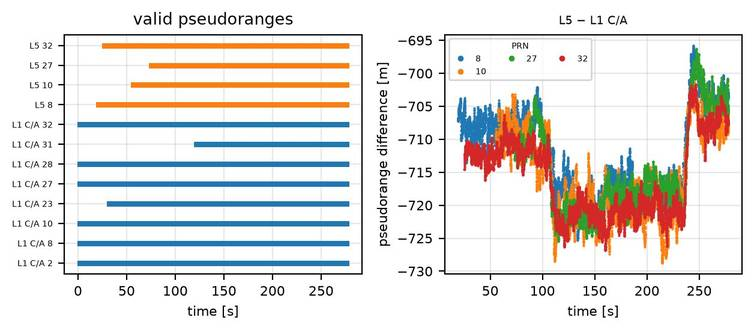
\includegraphics[width=1.0\linewidth]{gnss_sdr/x310_20261026T190001Z/observables.jpg}
  \caption{Observables: epochs with a valid pseudorange per band and satellite, and the difference between the two bands' pseudoranges of the same satellite (a constant receiver inter-band bias, the same for every satellite, plus the slowly varying ionospheric delay).}
\end{figure}

\begin{table}[H]
  \centering
  \footnotesize
  \resizebox{\ifdim\width>\linewidth\linewidth\else\width\fi}{!}{%
  \begin{tabular}{lrrrrrr}
    \hline
    \textbf{Difference} & \textbf{PRN} & \textbf{Common epochs} & \textbf{of run [\%]} & \textbf{Mean [m]} & \textbf{Std [m]} & \textbf{Drift [m/s]} \\
    \hline
    L5 $-$ L1 C/A & 8 & 12444 & 83 & -712.46 & 6.49 & -0.0031 \\
    L5 $-$ L1 C/A & 10 & 10772 & 72 & -715.60 & 6.47 & 0.0076 \\
    L5 $-$ L1 C/A & 27 & 9977 & 67 & -714.78 & 7.17 & 0.0509 \\
    L5 $-$ L1 C/A & 32 & 12166 & 81 & -715.94 & 6.04 & 0.0013 \\
    \hline
  \end{tabular}}
  \caption{Observables: pseudorange difference between the two bands of each satellite at common epochs (similar means = shared receiver bias; std = code noise of both bands).}
\end{table}

\subsubsection{PVT}
Position from the pseudoranges and the decoded ephemeris, compared with the surveyed antenna position (-23.209433$^\circ$, -45.874875$^\circ$, 596.42~m).

\begin{figure}[H]
  \centering
  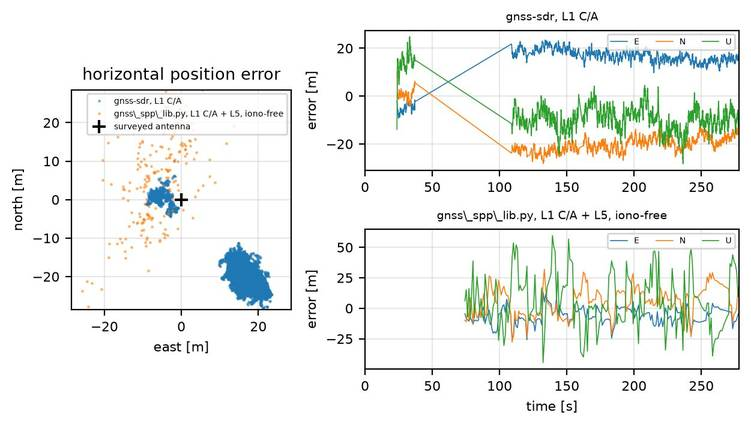
\includegraphics[width=1.0\linewidth]{gnss_sdr/x310_20261026T190001Z/pvt.jpg}
  \caption{PVT: position error of GNSS-SDR's own RTKLIB solution with respect to the surveyed antenna position (single frequency, broadcast ionosphere model).}
\end{figure}

\begin{table}[H]
  \centering
  \footnotesize
  \resizebox{\ifdim\width>\linewidth\linewidth\else\width\fi}{!}{%
  \begin{tabular}{l>{\centering\arraybackslash}p{4.2cm}}
    \hline
    \textbf{Solution} & \textbf{gnss-sdr, L1 C/A} \\
    \hline
    Solutions & 8879 \\
    Run with fix [\%] & 66 \\
    Mean E / N / U [m] & 15.2 / -18.6 / -7.8 \\
    Std E / N / U [m] & 6.3 / 6.1 / 7.9 \\
    RMS 2-D [m] & 25.6 \\
    RMS 3-D [m] & 27.9 \\
    95\% horiz. [m] & 31.8 \\
    \hline
  \end{tabular}}
  \caption{PVT: position error statistics with respect to the surveyed antenna (mean = accuracy, std = precision; \% of the run's seconds with a position; GNSS-SDR outputs several solutions per second).}
\end{table}


\subsubsection{Signal conditioner}


\begin{table}[H]
  \centering
  \footnotesize
  \resizebox{\ifdim\width>\linewidth\linewidth\else\width\fi}{!}{%
  \begin{tabular}{l>{\centering\arraybackslash}p{4.2cm}>{\centering\arraybackslash}p{4.2cm}}
    \hline
    \textbf{Channel} & \textbf{ch0 (E1)} & \textbf{ch1 (E5a)} \\
    \hline
    File format & ci8 & ci8 \\
    Source item type & ibyte & ibyte \\
    Data type adapter & Ibyte\_To\_Complex & Ibyte\_To\_Complex \\
    Input filter & Pass\_Through & Pass\_Through \\
    Resampling & $\times$5 zero-order hold, offline (\texttt{upsample\_iq.py}) & Pass\_Through \\
    Rate [MS/s] & 4 $\to$ 20 & 20 $\to$ 20 \\
    \hline
  \end{tabular}}
  \caption{Signal conditioner: recorded format and rate to gnss-sdr's internal \texttt{gr\_complex} stream; both bands are read in lockstep by one \texttt{Multichannel\_File\_Signal\_Source}.}
\end{table}

\subsubsection{Acquisition}
Two-dimensional search over code delay and Doppler (one channel per band dumped; the others behave alike).

\begin{figure}[H]
  \centering
  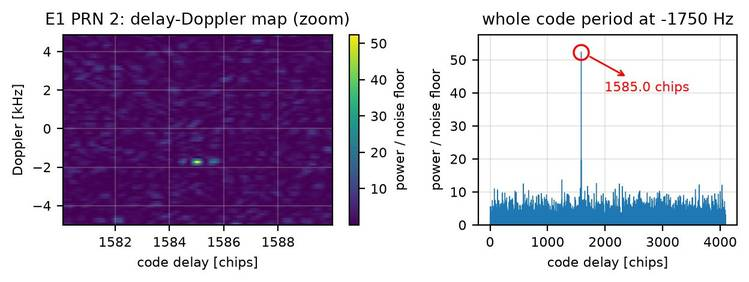
\includegraphics[width=1.0\linewidth]{gnss_sdr/x310_20261026T190001Z/galileo_acq_1B.jpg}
  \caption{Acquisition, E1: delay--Doppler search of PRN 2; one sharp peak (test statistic 73 vs threshold 52) at -1750~Hz and 1585.0~chips.}
\end{figure}

\begin{figure}[H]
  \centering
  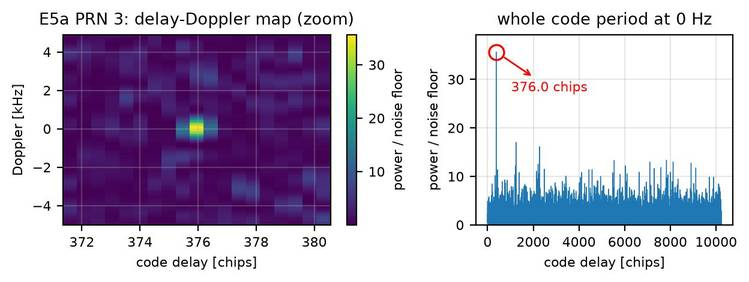
\includegraphics[width=1.0\linewidth]{gnss_sdr/x310_20261026T190001Z/galileo_acq_5X.jpg}
  \caption{Acquisition, E5a: delay--Doppler search of PRN 3; one sharp peak (test statistic 49 vs threshold 49) at 2223~Hz and 376.0~chips.}
\end{figure}

\begin{table}[H]
  \centering
  \footnotesize
  \resizebox{\ifdim\width>\linewidth\linewidth\else\width\fi}{!}{%
  \begin{tabular}{lrrrr}
    \hline
    \textbf{Band} & \textbf{Attempts} & \textbf{Detections} & \textbf{Detected PRNs} & \textbf{Best statistic / threshold\footnotemark} \\
    \hline
    E1 & 7 & 1 & 2 & 1.4 \\
    E5a & 74 & 1 & 3 & 1.0 \\
    \hline
  \end{tabular}}
  \caption{Acquisition: search attempts of the dumped channel. Attempts on satellites that are not in view (or do not broadcast that signal, e.g. older GPS satellites on L5/L2C) are rejected below the threshold.}
\end{table}

\footnotetext{Margin of the band's strongest detection: the largest acquisition test statistic among the detected attempts (the correlation peak of the delay--Doppler grid, normalised by the power of the input samples searched, i.e. the noise power, since GNSS signals are below the noise) divided by the detection threshold, which GNSS-SDR derives from the configured probability of false alarm. A value of 1 is right at the detection limit; e.g. 2.5 means the peak cleared the threshold 2.5 times over.}

\subsubsection{Tracking}


\begin{figure}[H]
  \centering
  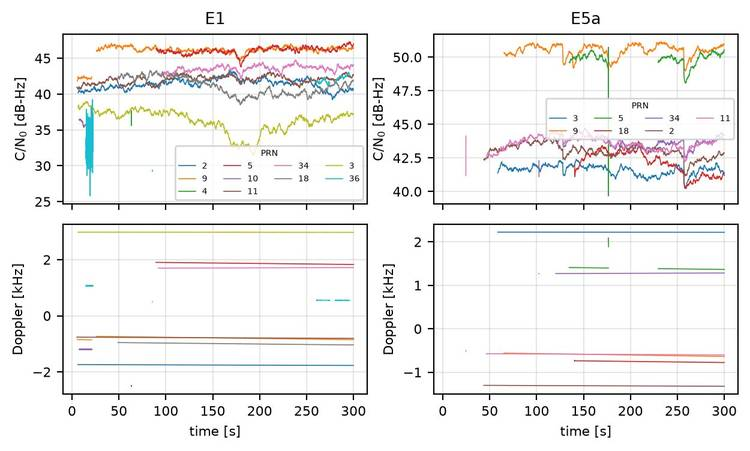
\includegraphics[width=1.0\linewidth]{gnss_sdr/x310_20261026T190001Z/galileo_tracking.jpg}
  \caption{Tracking: carrier-to-noise density ratio and carrier Doppler per satellite, while phase-locked (smooth Doppler curves = loops following the real satellite motion).}
\end{figure}

\begin{figure}[H]
  \centering
  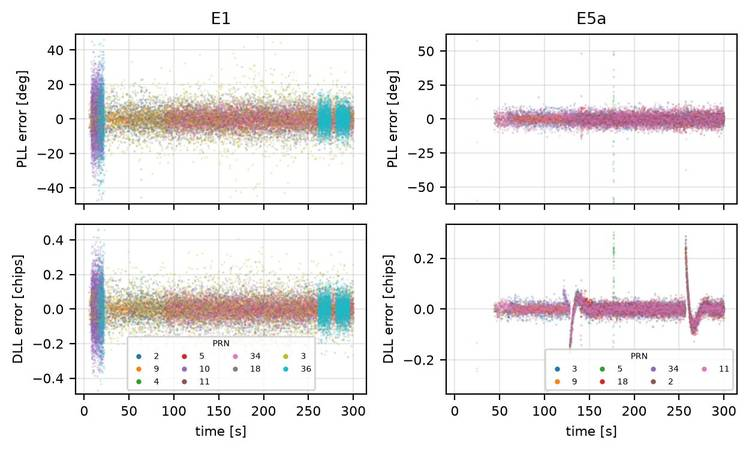
\includegraphics[width=1.0\linewidth]{gnss_sdr/x310_20261026T190001Z/galileo_tracking_errors.jpg}
  \caption{Tracking: loop errors per satellite while phase-locked, i.e. the discriminator outputs that the loops drive to zero: PLL carrier-phase error (degrees) and DLL code-delay error (chips) of every correlation. Noise centred on zero = clean tracking; its spread grows as C/N$_0$ drops, and jumps would mark cycle slips or a loop losing lock.}
\end{figure}

\begin{figure}[H]
  \centering
  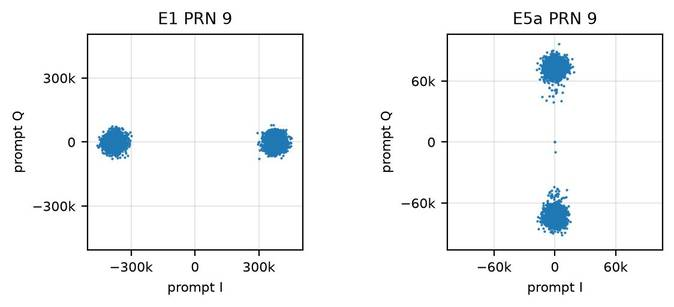
\includegraphics[width=1.0\linewidth]{gnss_sdr/x310_20261026T190001Z/galileo_tracking_iq.jpg}
  \caption{Tracking: prompt correlator outputs of the strongest satellite per band. Two tight clusters on one axis (the $\pm1$ data bits; GNSS-SDR's L5 tracking puts the data component on the Q axis), or, for the dataless pilots tracked for Galileo (E1-C, E5a-Q), the $\pm1$ chips of their secondary code, mean the PLL is phase-locked; a ring would mean it is not. \texttt{Prompt\_I}/\texttt{Prompt\_Q} are 32-bit floats (sums of the samples over one integration period, in file units): they never clip, only overflowing beyond $\pm 3.4\times10^{38}$, far above the $N\cdot\text{full scale}\cdot\sqrt{2}$ a sum of $N$ samples can reach.}
\end{figure}

\begin{table}[H]
  \centering
  \footnotesize
  \resizebox{\ifdim\width>\linewidth\linewidth\else\width\fi}{!}{%
  \begin{tabular}{lrrrrrrrr}
    \hline
    \textbf{Band} & \textbf{Ch.} & \textbf{PRN} & \textbf{Median C/N$_0$ [dB-Hz]} & \textbf{Phase-locked [\%]} & \textbf{Losses of lock} & \textbf{Tracked [s]} & \textbf{PLL error std [deg]} & \textbf{DLL error std [chips]} \\
    \hline
    E1 & 0 & 2 & 41.4 & 98 & 0 & 298 & 6.2 & 0.066 \\
    E1 & 1 & 9 & 46.2 & 97 & 1 & 300 & 3.3 & 0.037 \\
    E1 & 2 & 4 & 38.5 & 1 & 4 & 63 & 57.4 & 0.106 \\
    E1 & 2 & 5 & 46.1 & 98 & 4 & 216 & 3.6 & 0.040 \\
    E1 & 2 & 10 & 36.2 & 64 & 4 & 21 & 12.3 & 0.125 \\
    E1 & 3 & 11 & 42.1 & 98 & 0 & 300 & 6.1 & 0.062 \\
    E1 & 4 & 34 & 43.3 & 70 & 4 & 299 & 4.9 & 0.052 \\
    E1 & 5 & 18 & 41.0 & 84 & 2 & 299 & 6.5 & 0.071 \\
    E1 & 6 & 3 & 36.7 & 98 & 0 & 298 & 11.9 & 0.121 \\
    E1 & 7 & 36 & 44.5 & 12 & 14 & 299 & 9.2 & 0.089 \\
    E5a & 8 & 3 & 41.6 & 51 & 0 & 263 & 3.8 & 0.033 \\
    E5a & 9 & 9 & 50.7 & 50 & 0 & 258 & 1.4 & 0.027 \\
    E5a & 10 & 5 & 34.1 & 10 & 3 & 185 & 8.0 & 0.043 \\
    E5a & 11 & 18 & 42.1 & 42 & 0 & 171 & 4.4 & 0.033 \\
    E5a & 12 & 34 & 43.7 & 44 & 0 & 198 & 2.9 & 0.035 \\
    E5a & 13 & 2 & 42.8 & 53 & 0 & 275 & 3.2 & 0.029 \\
    E5a & 15 & 11 & 43.1 & 52 & 0 & 275 & 4.5 & 0.030 \\
    \hline
  \end{tabular}}
  \caption{Tracking: per channel and satellite (phase-locked: carrier lock test $> 0.8$; loop error standard deviations while phase-locked).}
\end{table}

\subsubsection{Telemetry decoder}


\begin{figure}[H]
  \centering
  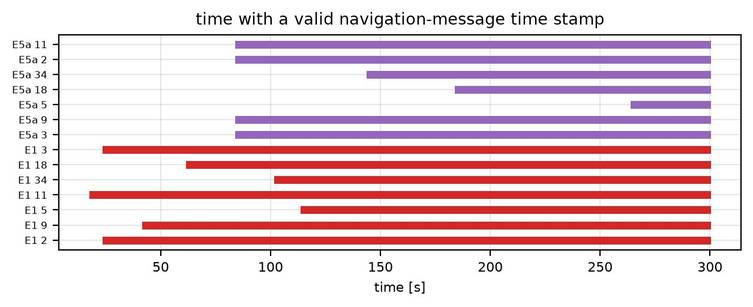
\includegraphics[width=1.0\linewidth]{gnss_sdr/x310_20261026T190001Z/galileo_telemetry.jpg}
  \caption{Telemetry decoder: per band and satellite, when the decoder delivered a valid transmit time (the first one comes after the first complete frame/message).}
\end{figure}

\begin{table}[H]
  \centering
  \footnotesize
  \resizebox{\ifdim\width>\linewidth\linewidth\else\width\fi}{!}{%
  \begin{tabular}{lrrrrr}
    \hline
    \textbf{Band} & \textbf{PRN} & \textbf{Messages decoded} & \textbf{Ephemeris} & \textbf{First valid at [s]} & \textbf{TOW [s]} \\
    \hline
    E1 & 2 & 27 & yes & 23.8 & 154850.0 \\
    E1 & 3 & 25 & yes & 23.8 & 154850.0 \\
    E1 & 5 & 18 & yes & 113.8 & 154940.0 \\
    E1 & 9 & 25 & yes & 41.8 & 154868.0 \\
    E1 & 11 & 27 & yes & 17.8 & 154844.0 \\
    E1 & 18 & 24 & yes & 61.8 & 154888.0 \\
    E1 & 34 & 19 & yes & 101.8 & 154928.0 \\
    E5a & 2 & 12 & yes & 84.1 & 154910.3 \\
    E5a & 3 & 12 & yes & 84.1 & 154910.3 \\
    E5a & 5 & 1 & yes & 264.0 & 155090.3 \\
    E5a & 9 & 12 & yes & 84.0 & 154910.3 \\
    E5a & 11 & 12 & yes & 84.0 & 154910.3 \\
    E5a & 18 & 4 & yes & 184.0 & 155010.3 \\
    E5a & 34 & 8 & yes & 144.1 & 154970.3 \\
    \hline
  \end{tabular}}
  \caption{Telemetry decoder: E1 I/NAV words, E5a F/NAV pages decoded, ephemeris obtained, and the first valid time of week.}
\end{table}

\subsubsection{Observables}
Pseudorange, carrier phase and Doppler of every channel at common receiver epochs.

\begin{figure}[H]
  \centering
  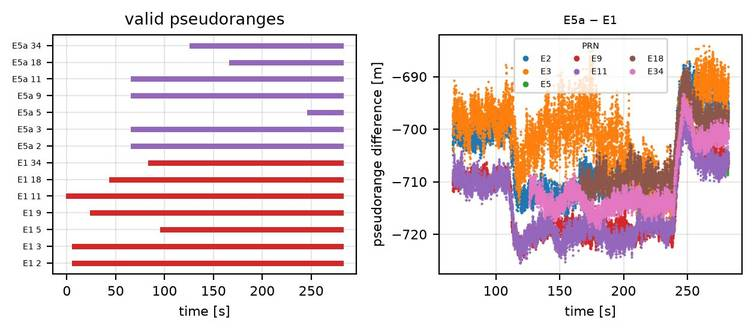
\includegraphics[width=1.0\linewidth]{gnss_sdr/x310_20261026T190001Z/galileo_observables.jpg}
  \caption{Observables: epochs with a valid pseudorange per band and satellite, and the difference between the two bands' pseudoranges of the same satellite (a constant receiver inter-band bias, the same for every satellite, plus the slowly varying ionospheric delay).}
\end{figure}

\begin{table}[H]
  \centering
  \footnotesize
  \resizebox{\ifdim\width>\linewidth\linewidth\else\width\fi}{!}{%
  \begin{tabular}{lrrrrrr}
    \hline
    \textbf{Difference} & \textbf{PRN} & \textbf{Common epochs} & \textbf{of run [\%]} & \textbf{Mean [m]} & \textbf{Std [m]} & \textbf{Drift [m/s]} \\
    \hline
    E5a $-$ E1 & 2 & 9649 & 64 & -705.48 & 7.29 & 0.0272 \\
    E5a $-$ E1 & 3 & 9649 & 64 & -700.47 & 6.77 & 0.0028 \\
    E5a $-$ E1 & 5 & 1769 & 12 & -703.48 & 2.96 & -0.2477 \\
    E5a $-$ E1 & 9 & 9649 & 64 & -714.02 & 6.79 & 0.0259 \\
    E5a $-$ E1 & 11 & 9649 & 64 & -714.54 & 6.51 & 0.0227 \\
    E5a $-$ E1 & 18 & 5271 & 35 & -704.75 & 6.76 & 0.1565 \\
    E5a $-$ E1 & 34 & 7027 & 47 & -710.08 & 6.21 & 0.0963 \\
    \hline
  \end{tabular}}
  \caption{Observables: pseudorange difference between the two bands of each satellite at common epochs (similar means = shared receiver bias; std = code noise of both bands).}
\end{table}

\subsubsection{PVT}
Position from the pseudoranges and the decoded ephemeris, compared with the surveyed antenna position (-23.209433$^\circ$, -45.874875$^\circ$, 596.42~m).

\begin{figure}[H]
  \centering
  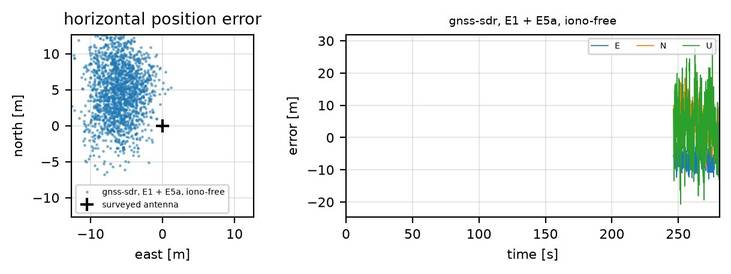
\includegraphics[width=1.0\linewidth]{gnss_sdr/x310_20261026T190001Z/galileo_pvt.jpg}
  \caption{PVT: position error of GNSS-SDR's own RTKLIB solution with respect to the surveyed antenna position.}
\end{figure}

\begin{table}[H]
  \centering
  \footnotesize
  \resizebox{\ifdim\width>\linewidth\linewidth\else\width\fi}{!}{%
  \begin{tabular}{l>{\centering\arraybackslash}p{4.2cm}}
    \hline
    \textbf{Solution} & \textbf{gnss-sdr, E1 + E5a, iono-free} \\
    \hline
    Solutions & 1732 \\
    Run with fix [\%] & 13 \\
    Mean E / N / U [m] & -6.0 / 4.9 / 3.0 \\
    Std E / N / U [m] & 2.3 / 4.1 / 8.1 \\
    RMS 2-D [m] & 9.0 \\
    RMS 3-D [m] & 12.5 \\
    95\% horiz. [m] & 13.7 \\
    \hline
  \end{tabular}}
  \caption{PVT: position error statistics with respect to the surveyed antenna (mean = accuracy, std = precision; \% of the run's seconds with a position; GNSS-SDR outputs several solutions per second).}
\end{table}




\subsection{Second record}
\begin{table}[H]
  \centering
  \begin{tabular}{|l|l|l|}
    \hline
    \textbf{Parameter} & \textbf{Channel 0} & \textbf{Channel 1} \\
    \hline
    Start time & \multicolumn{2}{>{\centering\arraybackslash}p{7cm}|}{2026-10-26 19:30:07 UTC} \\
    \hline
    Frequency & 1575.420 MHz (L1) & 1227.600 MHz (L2) \\
    \hline
    Duration & 300.0 s & 300.0 s \\
    \hline
    Sample rate & 4.000 MS/s & 4.000 MS/s \\
    \hline
    Sample type & \multicolumn{2}{>{\centering\arraybackslash}p{7cm}|}{signed complex 16-bit samples (I+Q), little-endian, as received from the X310 (sc16)} \\
    \hline
    Gain & 25.0 dB & 25.0 dB \\
    \hline
    Antenna & RX1 & RX2 \\
    \hline
    File size & 4800.0 MB & 4800.0 MB \\
    \hline
    Samples written & 1,200,000,000 & 1,200,000,000 \\
    \hline
    Lost samples & 0 & 0 \\
    \hline
    Clock source & \multicolumn{2}{>{\centering\arraybackslash}p{7cm}|}{external} \\
    \hline
    Time source & \multicolumn{2}{>{\centering\arraybackslash}p{7cm}|}{internal} \\
    \hline
    Motherboard & \multicolumn{2}{>{\centering\arraybackslash}p{7cm}|}{USRP X310} \\
    \hline
    Daughterboard & TwinRX RX0 & TwinRX RX1 \\
    \hline
    Recorder & \multicolumn{2}{>{\centering\arraybackslash}p{7cm}|}{UHD Python API} \\
    \hline
    GNSS-SDR configuration & \multicolumn{2}{>{\centering\arraybackslash}p{7cm}|}{\texttt{l1ca16bits4msps\_l2c16bits4msps.conf}} \\
    \hline
  \end{tabular}
  \caption{Metadata for recording \texttt{x310\_20261026T193001Z}, captured starting 2026-10-26T19:30:07.793328Z.}
\end{table}

\subsubsection{Signal source}
Raw I/Q samples of each channel analysed within the window [10, 10.5]~s after the start recording instant.

\begin{figure}[H]
  \centering
  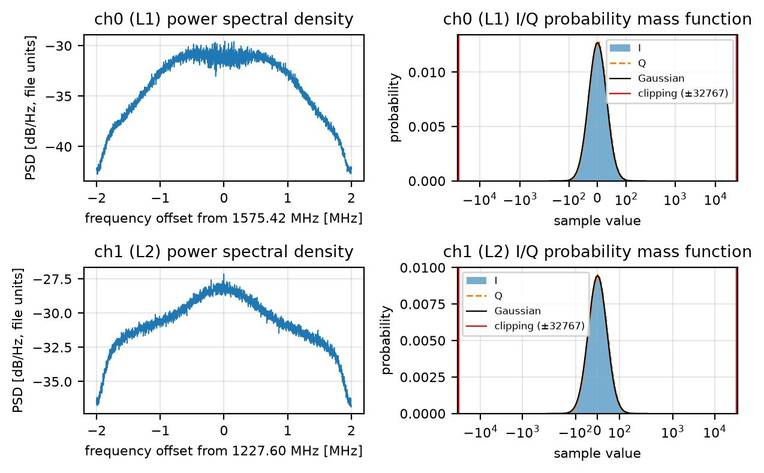
\includegraphics[width=1.0\linewidth]{gnss_sdr/x310_20261026T193001Z/source.jpg}
  \caption{Signal source: power spectral density (the receiver passband over a flat thermal-noise floor; GNSS signals are below the noise, so only interference would stand out) and probability mass functions of the integer I/Q sample values (Gaussian noise, centred, not clipped).}
\end{figure}

\begin{table}[H]
  \centering
  \footnotesize
  \resizebox{\ifdim\width>\linewidth\linewidth\else\width\fi}{!}{%
  \begin{tabular}{l>{\centering\arraybackslash}p{4.2cm}>{\centering\arraybackslash}p{4.2cm}}
    \hline
    \textbf{Channel} & \textbf{ch0} & \textbf{ch1} \\
    \hline
    Frequency [MHz] & 1575.42 & 1227.60 \\
    Rate [MS/s] & 4 & 4 \\
    Format & ci16\_le & ci16\_le \\
    Bytes per complex sample & 4 (2 for I, 2 for Q) & 4 (2 for I, 2 for Q) \\
    Full scale & $\pm$32767 & $\pm$32767 \\
    Gain [dB] & 25 & 25 \\
    Std I / Q & 31.4 / 31.4 & 42.3 / 42.3 \\
    Mean I / Q & -0.07 / -0.04 & 0.22 / 0.09 \\
    Min / max I & -162 / 151 & -222 / 203 \\
    Min / max Q & -149 / 149 & -202 / 210 \\
    Headroom\footnotemark & 1043.8 & 774.6 \\
    Clipped [\%] & 0.000 & 0.000 \\
    Lost samples & 0 & 0 \\
    \hline
  \end{tabular}}
  \caption{Signal source: sample statistics per channel (headroom: how many standard deviations of the noise fit before clipping).}
\end{table}

\footnotetext{Headroom $= A/\sigma$, where $A$ is the full scale of the sample format (127 for 8-bit, 32767 for 16-bit) and $\sigma$ the standard deviation of the I and Q samples together (both in file units, over the analysed window). For Gaussian noise, the fraction of clipped values is $2Q(A/\sigma)$, with $Q$ the Gaussian tail function: e.g. 0.003\,\% at $4.2\sigma$.}

\subsubsection{Signal conditioner}


\begin{table}[H]
  \centering
  \footnotesize
  \resizebox{\ifdim\width>\linewidth\linewidth\else\width\fi}{!}{%
  \begin{tabular}{l>{\centering\arraybackslash}p{4.2cm}>{\centering\arraybackslash}p{4.2cm}}
    \hline
    \textbf{Channel} & \textbf{ch0 (L1 C/A, E1)} & \textbf{ch1 (L2C)} \\
    \hline
    File format & ci16\_le & ci16\_le \\
    Source item type & ishort & ishort \\
    Data type adapter & Ishort\_To\_Complex & Ishort\_To\_Complex \\
    Input filter & Pass\_Through & Pass\_Through \\
    Resampling & Pass\_Through & Pass\_Through \\
    Rate [MS/s] & 4 $\to$ 4 & 4 $\to$ 4 \\
    \hline
  \end{tabular}}
  \caption{Signal conditioner: recorded format and rate to gnss-sdr's internal \texttt{gr\_complex} stream; both bands are read in lockstep by one \texttt{Multichannel\_File\_Signal\_Source}.}
\end{table}

\subsubsection{Acquisition}
Two-dimensional search over code delay and Doppler (one channel per band dumped; the others behave alike).

\begin{figure}[H]
  \centering
  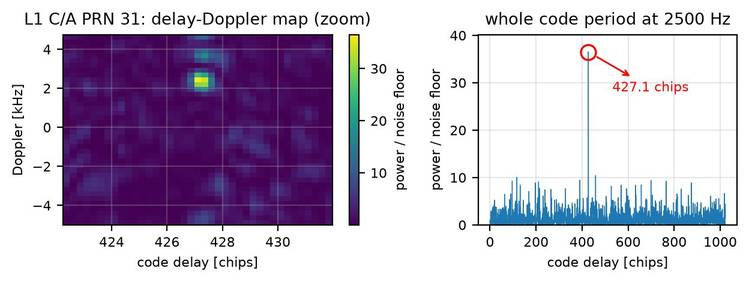
\includegraphics[width=1.0\linewidth]{gnss_sdr/x310_20261026T193001Z/acq_1C.jpg}
  \caption{Acquisition, L1 C/A: delay--Doppler search of PRN 31; one sharp peak (test statistic 51 vs threshold 44) at 2500~Hz and 427.1~chips.}
\end{figure}

\begin{figure}[H]
  \centering
  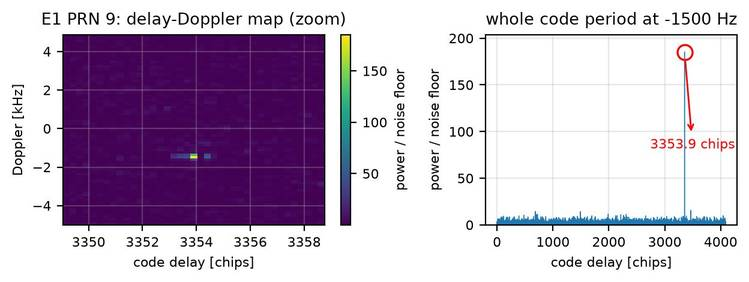
\includegraphics[width=1.0\linewidth]{gnss_sdr/x310_20261026T193001Z/acq_1B.jpg}
  \caption{Acquisition, E1: delay--Doppler search of PRN 9; one sharp peak (test statistic 263 vs threshold 48) at -1500~Hz and 3353.9~chips.}
\end{figure}

\begin{table}[H]
  \centering
  \footnotesize
  \resizebox{\ifdim\width>\linewidth\linewidth\else\width\fi}{!}{%
  \begin{tabular}{lrrrr}
    \hline
    \textbf{Band} & \textbf{Attempts} & \textbf{Detections} & \textbf{Detected PRNs} & \textbf{Best statistic / threshold\footnotemark} \\
    \hline
    L1 C/A & 26 & 1 & 31 & 1.2 \\
    L2C & \multicolumn{4}{l}{not dumped (search grid too large); acquired satellites: see the tracking table} \\
    E1 & 2 & 2 & 9 & 5.4 \\
    \hline
  \end{tabular}}
  \caption{Acquisition: search attempts of the dumped channel. Attempts on satellites that are not in view (or do not broadcast that signal, e.g. older GPS satellites on L5/L2C) are rejected below the threshold.}
\end{table}

\footnotetext{Margin of the band's strongest detection: the largest acquisition test statistic among the detected attempts (the correlation peak of the delay--Doppler grid, normalised by the power of the input samples searched, i.e. the noise power, since GNSS signals are below the noise) divided by the detection threshold, which GNSS-SDR derives from the configured probability of false alarm. A value of 1 is right at the detection limit; e.g. 2.5 means the peak cleared the threshold 2.5 times over.}

\subsubsection{Tracking}


\begin{figure}[H]
  \centering
  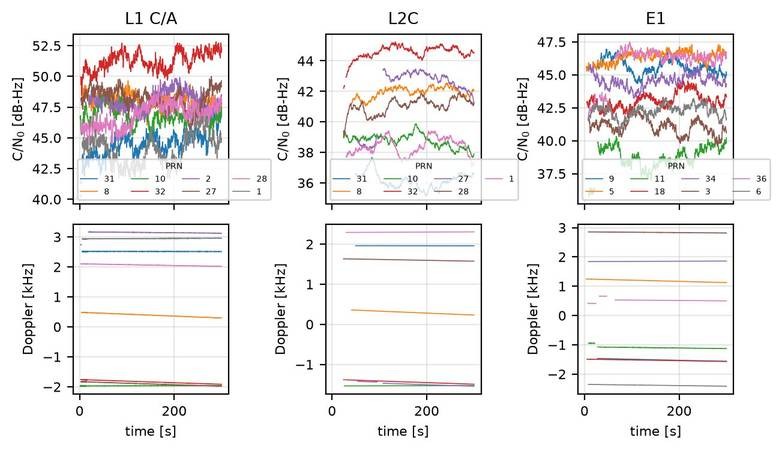
\includegraphics[width=1.0\linewidth]{gnss_sdr/x310_20261026T193001Z/tracking.jpg}
  \caption{Tracking: carrier-to-noise density ratio and carrier Doppler per satellite, while phase-locked (smooth Doppler curves = loops following the real satellite motion).}
\end{figure}

\begin{figure}[H]
  \centering
  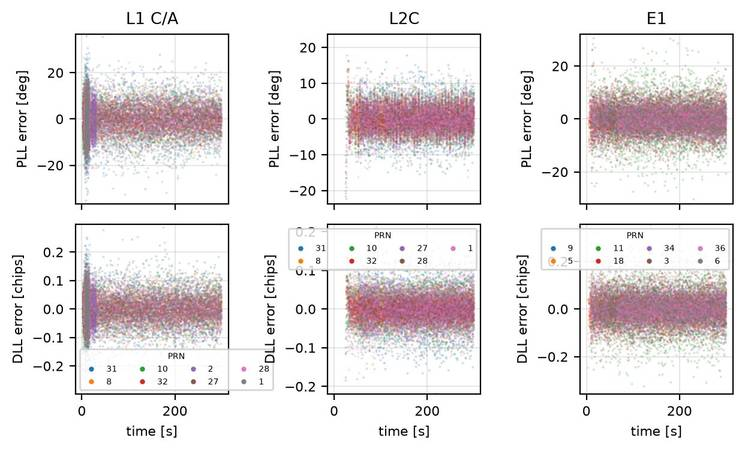
\includegraphics[width=1.0\linewidth]{gnss_sdr/x310_20261026T193001Z/tracking_errors.jpg}
  \caption{Tracking: loop errors per satellite while phase-locked, i.e. the discriminator outputs that the loops drive to zero: PLL carrier-phase error (degrees) and DLL code-delay error (chips) of every correlation. Noise centred on zero = clean tracking; its spread grows as C/N$_0$ drops, and jumps would mark cycle slips or a loop losing lock.}
\end{figure}

\begin{figure}[H]
  \centering
  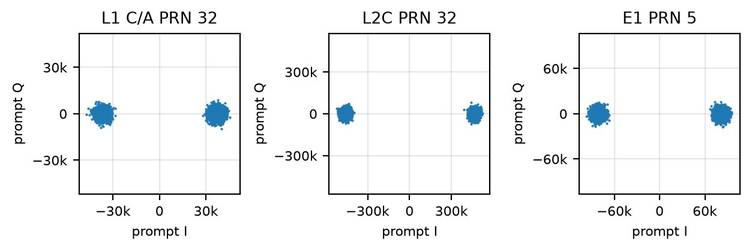
\includegraphics[width=1.0\linewidth]{gnss_sdr/x310_20261026T193001Z/tracking_iq.jpg}
  \caption{Tracking: prompt correlator outputs of the strongest satellite per band. Two tight clusters on one axis (the $\pm1$ data bits; GNSS-SDR's L5 tracking puts the data component on the Q axis), or, for the dataless pilots tracked for Galileo (E1-C, E5a-Q), the $\pm1$ chips of their secondary code, mean the PLL is phase-locked; a ring would mean it is not. \texttt{Prompt\_I}/\texttt{Prompt\_Q} are 32-bit floats (sums of the samples over one integration period, in file units): they never clip, only overflowing beyond $\pm 3.4\times10^{38}$, far above the $N\cdot\text{full scale}\cdot\sqrt{2}$ a sum of $N$ samples can reach.}
\end{figure}

\begin{table}[H]
  \centering
  \footnotesize
  \resizebox{\ifdim\width>\linewidth\linewidth\else\width\fi}{!}{%
  \begin{tabular}{lrrrrrrrr}
    \hline
    \textbf{Band} & \textbf{Ch.} & \textbf{PRN} & \textbf{Median C/N$_0$ [dB-Hz]} & \textbf{Phase-locked [\%]} & \textbf{Losses of lock} & \textbf{Tracked [s]} & \textbf{PLL error std [deg]} & \textbf{DLL error std [chips]} \\
    \hline
    L1 C/A & 0 & 31 & 43.5 & 95 & 0 & 296 & 9.3 & 0.071 \\
    L1 C/A & 1 & 8 & 48.4 & 96 & 0 & 297 & 5.5 & 0.044 \\
    L1 C/A & 2 & 10 & 46.7 & 95 & 0 & 300 & 6.6 & 0.050 \\
    L1 C/A & 3 & 32 & 50.8 & 98 & 0 & 298 & 4.1 & 0.031 \\
    L1 C/A & 4 & 2 & 48.0 & 57 & 1 & 298 & 5.5 & 0.043 \\
    L1 C/A & 5 & 27 & 48.2 & 94 & 0 & 298 & 5.5 & 0.041 \\
    L1 C/A & 6 & 28 & 45.9 & 94 & 0 & 298 & 6.9 & 0.053 \\
    L1 C/A & 7 & 1 & 44.3 & 90 & 0 & 297 & 9.3 & 0.069 \\
    L2C & 8 & 31 & 36.2 & 91 & 0 & 276 & 5.1 & 0.056 \\
    L2C & 9 & 8 & 42.0 & 94 & 0 & 276 & 3.2 & 0.030 \\
    L2C & 10 & 10 & 38.8 & 99 & 0 & 276 & 4.2 & 0.044 \\
    L2C & 11 & 32 & 44.7 & 99 & 0 & 276 & 3.5 & 0.023 \\
    L2C & 12 & 27 & 42.7 & 85 & 1 & 276 & 3.1 & 0.031 \\
    L2C & 13 & 28 & 41.1 & 100 & 0 & 276 & 3.6 & 0.035 \\
    L2C & 14 & 1 & 38.4 & 98 & 0 & 276 & 4.3 & 0.046 \\
    E1 & 16 & 9 & 45.5 & 91 & 1 & 299 & 3.7 & 0.041 \\
    E1 & 17 & 5 & 46.4 & 100 & 0 & 296 & 3.7 & 0.041 \\
    E1 & 18 & 11 & 38.8 & 95 & 1 & 299 & 8.9 & 0.096 \\
    E1 & 19 & 18 & 43.0 & 99 & 0 & 299 & 5.3 & 0.060 \\
    E1 & 20 & 34 & 44.5 & 98 & 0 & 297 & 4.3 & 0.050 \\
    E1 & 21 & 3 & 41.1 & 98 & 0 & 297 & 6.6 & 0.075 \\
    E1 & 22 & 36 & 46.4 & 91 & 3 & 295 & 3.9 & 0.044 \\
    E1 & 23 & 6 & 42.3 & 99 & 0 & 296 & 5.4 & 0.064 \\
    \hline
  \end{tabular}}
  \caption{Tracking: per channel and satellite (phase-locked: carrier lock test $> 0.8$; loop error standard deviations while phase-locked).}
\end{table}

\subsubsection{Telemetry decoder}


\begin{figure}[H]
  \centering
  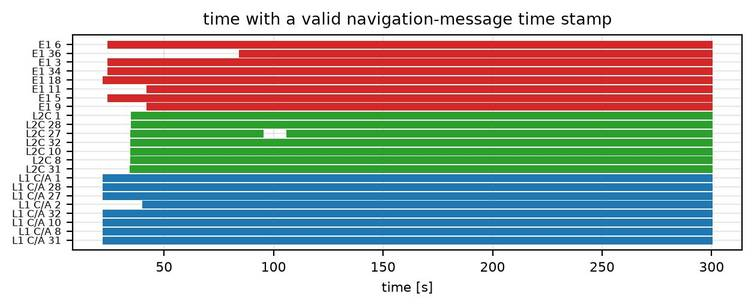
\includegraphics[width=1.0\linewidth]{gnss_sdr/x310_20261026T193001Z/telemetry.jpg}
  \caption{Telemetry decoder: per band and satellite, when the decoder delivered a valid transmit time (the first one comes after the first complete frame/message).}
\end{figure}

\begin{table}[H]
  \centering
  \footnotesize
  \resizebox{\ifdim\width>\linewidth\linewidth\else\width\fi}{!}{%
  \begin{tabular}{lrrrrr}
    \hline
    \textbf{Band} & \textbf{PRN} & \textbf{Messages decoded} & \textbf{Ephemeris} & \textbf{First valid at [s]} & \textbf{TOW [s]} \\
    \hline
    E1 & 3 & 26 & yes & 24.3 & 156650.0 \\
    E1 & 5 & 26 & yes & 24.3 & 156650.0 \\
    E1 & 6 & 26 & yes & 24.3 & 156650.0 \\
    E1 & 9 & 25 & yes & 42.3 & 156668.0 \\
    E1 & 11 & 25 & yes & 42.3 & 156668.0 \\
    E1 & 18 & 26 & yes & 22.3 & 156648.0 \\
    E1 & 34 & 26 & yes & 24.3 & 156650.0 \\
    E1 & 36 & 21 & yes & 84.3 & 156710.0 \\
    L1 C/A & 1 & 47 & yes & 22.3 & 156648.0 \\
    L1 C/A & 2 & 44 & yes & 40.3 & 156666.0 \\
    L1 C/A & 8 & 46 & yes & 22.3 & 156648.0 \\
    L1 C/A & 10 & 46 & yes & 22.3 & 156648.0 \\
    L1 C/A & 27 & 46 & yes & 22.3 & 156648.0 \\
    L1 C/A & 28 & 46 & yes & 22.3 & 156648.0 \\
    L1 C/A & 31 & 47 & yes & 22.3 & 156648.0 \\
    L1 C/A & 32 & 46 & yes & 22.3 & 156648.0 \\
    L2C & 1 & 15 & yes & 35.1 & 0.0 \\
    L2C & 8 & 13 & yes & 34.7 & 0.0 \\
    L2C & 10 & 13 & yes & 34.8 & 0.0 \\
    L2C & 27 & 9 & yes & 34.9 & 0.0 \\
    L2C & 28 & 15 & yes & 35.0 & 0.0 \\
    L2C & 31 & 13 & yes & 34.7 & 0.0 \\
    L2C & 32 & 13 & yes & 34.9 & 0.0 \\
    \hline
  \end{tabular}}
  \caption{Telemetry decoder: L1 C/A LNAV subframes, L2C CNAV messages, E1 I/NAV words decoded, ephemeris obtained, and the first valid time of week.}
\end{table}

\subsubsection{Observables}
Pseudorange, carrier phase and Doppler of every channel at common receiver epochs.

\begin{figure}[H]
  \centering
  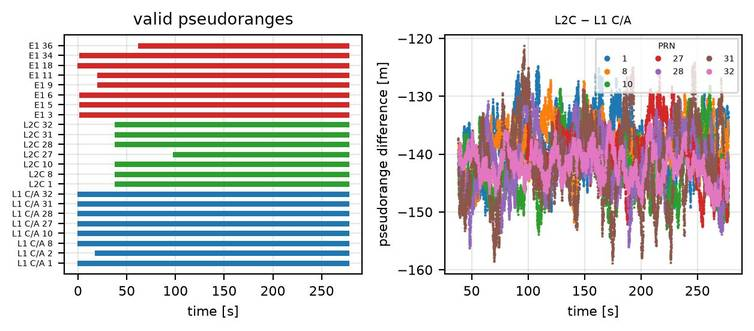
\includegraphics[width=1.0\linewidth]{gnss_sdr/x310_20261026T193001Z/observables.jpg}
  \caption{Observables: epochs with a valid pseudorange per band and satellite, and the difference between the two bands' pseudoranges of the same satellite (a constant receiver inter-band bias, the same for every satellite, plus the slowly varying ionospheric delay).}
\end{figure}

\begin{table}[H]
  \centering
  \footnotesize
  \resizebox{\ifdim\width>\linewidth\linewidth\else\width\fi}{!}{%
  \begin{tabular}{lrrrrrr}
    \hline
    \textbf{Difference} & \textbf{PRN} & \textbf{Common epochs} & \textbf{of run [\%]} & \textbf{Mean [m]} & \textbf{Std [m]} & \textbf{Drift [m/s]} \\
    \hline
    L2C $-$ L1 C/A & 1 & 11953 & 80 & -138.46 & 4.58 & 0.0012 \\
    L2C $-$ L1 C/A & 8 & 11970 & 80 & -138.63 & 3.59 & 0.0075 \\
    L2C $-$ L1 C/A & 10 & 11967 & 80 & -142.09 & 4.87 & 0.0069 \\
    L2C $-$ L1 C/A & 27 & 8972 & 60 & -139.85 & 4.53 & -0.0158 \\
    L2C $-$ L1 C/A & 28 & 11957 & 80 & -140.93 & 4.98 & 0.0068 \\
    L2C $-$ L1 C/A & 31 & 11973 & 80 & -141.25 & 6.69 & 0.0048 \\
    L2C $-$ L1 C/A & 32 & 11964 & 80 & -141.84 & 2.75 & -0.0096 \\
    \hline
  \end{tabular}}
  \caption{Observables: pseudorange difference between the two bands of each satellite at common epochs (similar means = shared receiver bias; std = code noise of both bands).}
\end{table}

\subsubsection{PVT}
Position from the pseudoranges and the decoded ephemeris, compared with the surveyed antenna position (-23.209433$^\circ$, -45.874875$^\circ$, 596.42~m).

\begin{figure}[H]
  \centering
  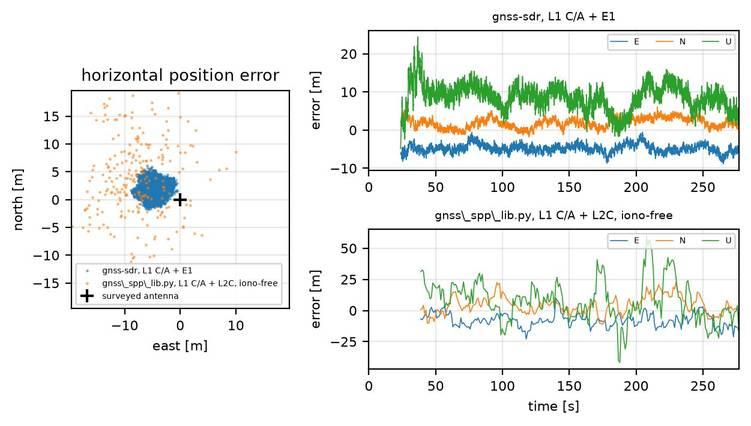
\includegraphics[width=1.0\linewidth]{gnss_sdr/x310_20261026T193001Z/pvt.jpg}
  \caption{PVT: position error with respect to the surveyed antenna position. gnss-sdr: GNSS-SDR's own RTKLIB solution (single frequency, broadcast ionosphere model). gnss\_spp\_lib.py: computed from gnss-sdr's observables and decoded GPS ephemeris, removing the ionospheric delay with the second band (pseudoranges carrier-smoothed over 100~s).}
\end{figure}

\begin{figure}[H]
  \centering
  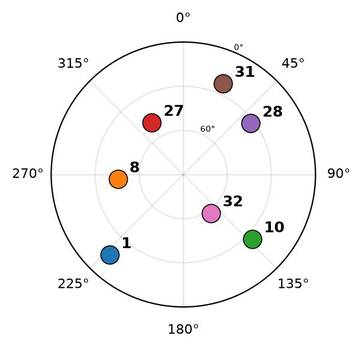
\includegraphics[width=0.45\linewidth]{gnss_sdr/x310_20261026T193001Z/skyplot.jpg}
  \caption{PVT: sky plot of the GPS satellites in the gnss\_spp\_lib.py dual-frequency solution (azimuth, elevation) during the recording.}
\end{figure}

\begin{table}[H]
  \centering
  \footnotesize
  \resizebox{\ifdim\width>\linewidth\linewidth\else\width\fi}{!}{%
  \begin{tabular}{l>{\centering\arraybackslash}p{4.2cm}>{\centering\arraybackslash}p{4.2cm}}
    \hline
    \textbf{Solution} & \textbf{gnss-sdr, L1 C/A + E1} & \textbf{gnss\_spp\_lib.py, L1 C/A + L2C, iono-free} \\
    \hline
    Solutions & 13178 & 239 \\
    Run with fix [\%] & 92 & 86 \\
    Mean E / N / U [m] & -4.8 / 1.9 / 8.6 & -7.8 / 4.2 / 8.0 \\
    Std E / N / U [m] & 1.1 / 1.3 / 3.3 & 5.3 / 7.0 / 16.6 \\
    RMS 2-D [m] & 5.4 & 12.5 \\
    RMS 3-D [m] & 10.7 & 22.3 \\
    95\% horiz. [m] & 7.2 & 20.8 \\
    \hline
  \end{tabular}}
  \caption{PVT: position error statistics with respect to the surveyed antenna (mean = accuracy, std = precision; \% of the run's seconds with a position; gnss-sdr outputs several solutions per second, gnss\_spp\_lib.py computes one per second).}
\end{table}




\part{Permanent scintillating data}
\label{part:permanent}

This part holds the recordings classified with moderate or strong scintillation (Section~\ref{sec:scintillation-classes}), which are kept in the permanent NAS storage. To keep the report small enough to be shared, each recording is shown with its metadata and its scintillation outputs only; the full GNSS-SDR outputs are shown while the recording is in Part~\ref{part:temporary}.

Table~\ref{tab:permanent-calendar} shows the days of the permanently stored recordings, with the same colors as the temporary calendar: \textcolor{green}{green} means 2 recordings, \textcolor{blue}{blue} means 1 recording, and no color means no recording was stored.

\begin{table}[H]
  \centering
  \begin{tabular}{ccc}
  \multicolumn{3}{c}{\textit{No recording stored yet.}} \\[2ex]
  \end{tabular}
  \caption{Permanent recording calendar.}
  \label{tab:permanent-calendar}
\end{table}

No recording has been classified and stored permanently yet.

\printbibliography

\end{document}
